% Gelfand seminar notes, 1979-80: source pages P000840-P000918.
% Russian diplomatic transcription (AI-made, checked against the scans), cut page by page from the cumulative working reader A4-reader-chapters01-34-complete-first1527-separated-diplomatic-r46.
% \SourcePage{GELFAND-Pnnnnnn}{label} starts a scanned page; the second argument is the number written
% on the page, if any. Editorial notes give the page, a label and the transcriber's remark; \Unclear
% marks a doubtful reading.
\SourcePage{GELFAND-P000840}{30}
\SourceFigure{GELFAND-P000840}{indexed-lines}{%
\begingroup\color{black}\GelfandFitDiagram{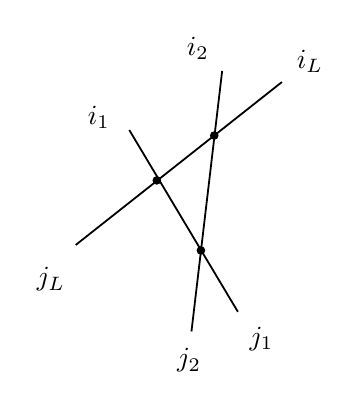
\begin{tikzpicture}[x=.01cm,y=-.01cm,line width=.65pt]
\draw (270,185)--(408,416) (388,110)--(349,441) (202,331)--(464,124);
\fill (305,249) circle[radius=.55mm];
\fill (378,192) circle[radius=.55mm];
\fill (361,338) circle[radius=.55mm];
\node[left] at (258,169) {\(i_1\)};
\node[above left] at (384,108) {\(i_2\)};
\node[above right] at (470,125) {\(i_L\)};
\node[below left] at (201,347) {\(j_L\)};
\node[below] at (346,450) {\(j_2\)};
\node[below right] at (410,423) {\(j_1\)};
\end{tikzpicture}}\endgroup}
\end{GelfandAdjacentEvidence}
\begin{GelfandAdjacentEvidence}{GELFAND-P000840}{2}


\uline{Ассоциат.}: \(Z\) не зав. от взаимного распол. прямых.

Достат., чтоб вып. для 3-х прямых:

\SourceFigure{GELFAND-P000840}{three-lines-equality}{%
\begingroup\color{black}\GelfandFitDiagram{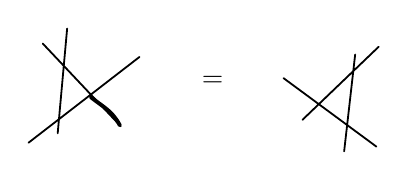
\begin{tikzpicture}[x=.010cm,y=-.010cm,line width=.65pt,line cap=round]
\draw (24,177)--(165,68) (42,51)--(141,156) (73,32)--(61,165);
\draw[line width=1.4pt] (103,119) .. controls (119,132) and (130,136) .. (140,155);
\node at (258,99) {\(=\)};
\draw (348,95)--(466,182) (372,148)--(469,55) (439,65)--(425,188);
\end{tikzpicture}}\endgroup\par
Утолщение на нисходящей линии слева может быть повторной обводкой или стрелкой.}
\end{GelfandAdjacentEvidence}
\begin{GelfandAdjacentEvidence}{GELFAND-P000840}{3}


\uline{Утв. 2.} сущ. такие матрицы.

\uwave{Об асимптотике}:

\begin{equation*}
\ln Z^{j_1\ldots j_L}_{i_1\ldots i_L}\sim L^2
\qquad\text{при }L\to\infty\tag{4}
\end{equation*}

(\uwave{если без ассоциативности}) и асимпт. не зав. от выбора инд. \(i\) и \(j\).

[Под «асимпт.»: (гл. член.)]

\uuline{Утв.} 3. Асимптотика при \(L\to\infty\)

\begin{equation*}
\ln Z(\lambda_1,\ldots,\lambda_L)
=\sum_{a>b=1}^{L}f(\lambda_a-\lambda_b)+\text{остат. член}\tag{5}
\end{equation*}
\Unclear{GELFAND-P000840}{asymptotic-index-limit}{Нижний предел записан «\(a>b=1\)». Верхний предел \(L\).}
\end{GelfandAdjacentEvidence}
\begin{GelfandAdjacentEvidence}{GELFAND-P000840}{4}


(своб. эн. большой системы \(=\) сумма парных

\uline{Мнение}: есть \(L\) сортов частиц; они движ. по прямым и сталкиваются; при столкн. они сохр. скорости, но меняют \uuline{цвет}
\Unclear{GELFAND-P000840}{particle-model-heading}{Заголовок предварительно прочитан «Мнение».}
\end{GelfandAdjacentEvidence}
\begin{GelfandAdjacentEvidence}{GELFAND-P000840}{5}

\Unclear{GELFAND-P000840}{modified-velocity-word}{Начальные штрихи слова «скорости» переправлены. Предшествующее начертание неразличимо.}
\end{GelfandAdjacentEvidence}
\begin{GelfandAdjacentEvidence}{GELFAND-P000840}{6}


[Под «цвет»: (сорт)]

Здесь \(Z\) — \(S\)-матрица;

Есть интерпр., когда \(Z\) — стат. сумма

Веса \(S\) — \(\exp\) от потенциала. (вероятности?)

Есть нач. и \uwave{конечные расцветки} \(i_1,\ldots,i_L\)
\[
j_1,\ldots,j_L.
\]

\SourceFigure{GELFAND-P000840}{particle-divider}{%
\begingroup\color{black}\GelfandFitDiagram{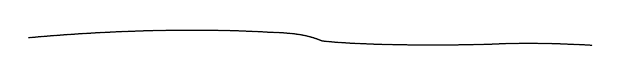
\begin{tikzpicture}[x=1cm,y=1cm,line width=.45pt]
\draw (0,0) .. controls (1.1,.10) and (2.2,.12) .. (3.06,.07)
 .. controls (3.41,.06) and (3.56,.03) .. (3.73,-.04)
 .. controls (4.13,-.09) and (5.23,-.11) .. (6.05,-.075)
 .. controls (6.48,-.063) and (6.83,-.079) .. (7.16,-.095);
\end{tikzpicture}}\endgroup}
\end{GelfandAdjacentEvidence}
\begin{GelfandAdjacentEvidence}{GELFAND-P000840}{7}


\uuline{А. З.}

\SourceFigure{GELFAND-P000840}{spin-lines-diagram}{%
\begingroup\color{black}\GelfandFitDiagram{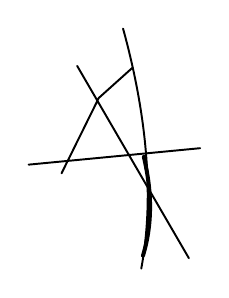
\begin{tikzpicture}[x=.011cm,y=-.011cm,line width=.7pt,line cap=round]
\draw (26,183)--(224,164) (82,69)--(211,291)
 (64,193)--(107,106)--(146,71);
\draw (135,26) .. controls (154,95) and (175,201) .. (156,303);
\draw[line width=1.45pt] (159,174) .. controls (165,200) and (172,242) .. (158,288);
\end{tikzpicture}}\endgroup\par
Два пересечения возле горизонтальной линии сливаются в утолщении. Длинная разделительная черта видна на отрывке слева.}
\end{GelfandAdjacentEvidence}
\begin{GelfandAdjacentEvidence}{GELFAND-P000840}{8}


\uwave{спиновые} \uwave{переменные} — в многоугольниках; взаимод. ближ. соседей;

\(S\) подбирается.
\Unclear{GELFAND-P000840}{s-expression-note}{Короткая приписка предварительно прочитана «подбирается». Начальные буквы и густой штрих остаются неясными.}
\end{GelfandAdjacentEvidence}


\[
Z=\sum_{\{\sigma\}}e^{-\beta H}
\qquad H=\sum h(\sigma_A,\sigma_B)
\]

Точно счит. стат. суммы — все такие!

\uline{Для модели Изинга}:
\[
S_{ij}^{k\ell}=\frac{ijk\ell+1}{2}e^{-\frac{\beta}{2}(i+j+k+\ell)}
\]

(после перехода к дуальной решётке)


\Needspace{7\baselineskip}
\begin{GelfandAdjacentEvidence}{GELFAND-P000841}{1}
\SourcePage{GELFAND-P000841}{unlabelled}
\uuline{24.9.79 г.}\qquad \uline{Сем. Гельфанда}

\uwave{Рената Эрнестовна КАЛЛОШ} о \uline{конфер. в Кембридже}

(физик)

(месячное раб. совещ. по кв. гравитации, прим. 40 чел.)

20 чел. из USA; в т. числе \uline{Chern, Singer, Milnor, Penrose};

Hawking, De Witt, Sciama, Coleman, Jackiw

[Под Hawking, с короткой вертикальной чертой:] претендент на св. кресло Ньютона
\Unclear{GELFAND-P000841}{newton-abbreviation}{Сокращение перед «кресло» предварительно прочитано «св.».}
\end{GelfandAdjacentEvidence}
\begin{GelfandAdjacentEvidence}{GELFAND-P000841}{2}


\uline{Gibbons} — физик, раб. с Хокингом — докл. о кв. гравитации
\Unclear{GELFAND-P000841}{gibbons-abbreviation}{Сокращение перед «о кв. гравитации» предварительно прочитано «докл.». Возможно «сем.».}
\end{GelfandAdjacentEvidence}
\begin{GelfandAdjacentEvidence}{GELFAND-P000841}{3}


\uwave{Идея}: надо принять во внимание эффекты нетрив. топологии пр-ва/времени в малом.

(много маленьких „ручек“).

Теория не построена, но есть значит. продвижения.

В основном \uwave{Hawking}:
\Unclear{GELFAND-P000841}{hawking-coauth-abbreviation}{Перед Hawking предварительно прочитано «В основном». Начальные штрихи второго слова слабы.}
\end{GelfandAdjacentEvidence}
\begin{GelfandAdjacentEvidence}{GELFAND-P000841}{4}


1) \uwave{Space-time foam} (пена) — вышло в \uwave{Nuclear Physics}

(обычн. журн.)
\Unclear{GELFAND-P000841}{journal-gloss}{Приписка под названием журнала предварительно прочитана «обычн. журн.».}
\end{GelfandAdjacentEvidence}
\begin{GelfandAdjacentEvidence}{GELFAND-P000841}{5}


2) \uwave{Page, Atiyah} \quad что-то в поле изв. гравитонов
\Unclear{GELFAND-P000841}{page-atiyah-abbreviation}{Сокращение предварительно прочитано «изв.». Возможно «изл.».}
\end{GelfandAdjacentEvidence}
\begin{GelfandAdjacentEvidence}{GELFAND-P000841}{6}


(из гр. Hawking)

3) \uwave{Coleman, Jackiw} \quad — о гравит. с учётом топ. чисел —

о Янге-Миллсе.

(есть обзор о методах инстантонов)
\Unclear{GELFAND-P000841}{instanton-gloss}{Предлог перед «методах» предварительно прочитан «о». Буква открыта и похожа на «с».}
\end{GelfandAdjacentEvidence}
\begin{GelfandAdjacentEvidence}{GELFAND-P000841}{7}


4) \uwave{Милнор} — классиф. 4-мерных мн-зий

Кто-то о рассл. на 4-мн-зиях.

5) \uwave{Зингер} — о сигнатуре 4-мн-зия.

\uwave{О супермногообразиях}

Счит. путём к квантованию

De Witt пишет книгу о супермн-зиях

Singer чит. лекции
\SourceFigure{GELFAND-P000841}{ditto-stroke}{%
\begingroup\color{black}\GelfandFitDiagram{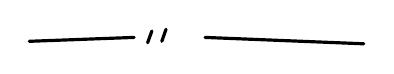
\begin{tikzpicture}[x=.9cm,y=.9cm,line width=1.15pt,line cap=round]
\draw (0,-.03)--(1.48,.025) (1.67,-.05)--(1.73,.115)
 (1.87,-.03)--(1.93,.14) (2.48,.025)--(4.72,-.065);
\end{tikzpicture}}\endgroup}
\end{GelfandAdjacentEvidence}
\begin{GelfandAdjacentEvidence}{GELFAND-P000841}{8}


\SourceFigure{GELFAND-P000841}{section-divider}{%
\begingroup\color{black}\GelfandFitDiagram{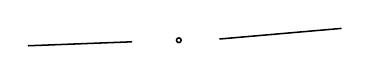
\begin{tikzpicture}[x=1cm,y=1cm,line width=.55pt,line cap=round]
\draw (0,-.06)--(1.31,-.01) (2.43,.026)--(3.97,.16);
\draw (1.91,.01) circle[radius=.03cm];
\end{tikzpicture}}\endgroup}
\end{GelfandAdjacentEvidence}
\begin{GelfandAdjacentEvidence}{GELFAND-P000841}{9}


\uwave{Нечто, что независ. получ. докладчицей и кем-то из участников конф.}

[Справа:] [Зачёркнуто: \sout{Christen[…]}] Christensen, Duff;
\Unclear{GELFAND-P000841}{cancelled-author}{Зачёркнутое имя предварительно прочитано «Christen[…]».}
\end{GelfandAdjacentEvidence}
\begin{GelfandAdjacentEvidence}{GELFAND-P000841}{10}


\uwave{Kallosh} — докладчица

Рассм. ур-е
\begin{equation*}
\Delta[A,B]\,\Phi[A,B]=0 \tag{1}
\end{equation*}

Здесь
\[
\phi[A,B]=\Psi_{\alpha_1\ldots\alpha_{2A},\,\dot\alpha_1,\ldots,\dot\alpha_{2B}}(x)
\]
— мультиспинор, преобр. по группе \(SO(4)\)
\Unclear{GELFAND-P000841}{group-symbol}{Вторая буква названия группы разомкнута. Предварительно набрано \(SO(4)\).}
\end{GelfandAdjacentEvidence}
\begin{GelfandAdjacentEvidence}{GELFAND-P000841}{11}


\(x\in\) [Зачёркнуто: \sout{…}] \(R^4\).
\Incomplete{GELFAND-P000841}{cancelled-space-symbol}{Перед \(R^4\) зачёркнут один знак. Его исходное начертание неразличимо.}
\end{GelfandAdjacentEvidence}
\begin{GelfandAdjacentEvidence}{GELFAND-P000841}{12}


\(\Delta\) — какой-то оператор; когда-то от Ходжа-де Рама.

здесь есть и пол. Дирака
\Unclear{GELFAND-P000841}{operator-gloss}{Сокращение перед «Дирака» предварительно прочитано «пол.».}
\end{GelfandAdjacentEvidence}
\begin{GelfandAdjacentEvidence}{GELFAND-P000841}{13}


\[
S=A+B,\qquad T=A-B.
\]

\begin{equation*}
n[S;T]-n[s;T-1]=4^{s-1}\left[\left(T-\frac12\right)\chi+\left(s-\frac13\right)\frac12p\right]
\tag{2}
\end{equation*}
\Unclear{GELFAND-P000841}{formula-two-s-case}{Формы \(S/s\) в (2) различаются по величине. Регистр не везде ясен.}
\end{GelfandAdjacentEvidence}


[Под \(n\), с короткой вертикальной чертой:] число 0-х мод

(разм. пр-ва реш., с спином \(A\) и \(B\));

\(\chi,p\) — числа Эйлера, Понтрягина


\Needspace{7\baselineskip}
\begin{GelfandAdjacentEvidence}{GELFAND-P000842}{1}
\SourcePage{GELFAND-P000842}{66}
Здесь есть теоремы Гаусса-Боне, Атья-Зингера, и т. п..

\begin{equation*}
n[A,B]-2n\left[A\overset{?}{-}\frac12,B\right]
=4^{A+B-1}\left(A-\frac7{12}\right)\left(\chi+\frac12p\right).
\tag{3}
\end{equation*}
\Unclear{GELFAND-P000842}{formula-three-sign}{Знак перед \(1/2\) густо затушёван. Минус — возможное чтение.}
\end{GelfandAdjacentEvidence}
\begin{GelfandAdjacentEvidence}{GELFAND-P000842}{2}


О ненулевых модах:

\begin{equation*}
m[S;T]=m[S]=4^s m[0]
\tag{4}
\end{equation*}
\Unclear{GELFAND-P000842}{formula-four-s-case}{Регистр \(s/S\) в показателе степени неясен. Последний аргумент предварительно набран цифрой \(0\).}
\end{GelfandAdjacentEvidence}
\begin{GelfandAdjacentEvidence}{GELFAND-P000842}{3}


[Под \(m[S;T]\):] ненулевые моды:

\begin{equation*}
\Delta\Psi_i=\lambda_i\Psi_i
\tag{5}
\end{equation*}

В супергравитации ненулевые моды сокращ. и ост. вклад лишь нулевых.

(3) [Зачёркнуто: \sout{…}] лишь если мн-зие \uwave{самодуально}.
\Incomplete{GELFAND-P000842}{selfduality-cancellation}{Слово под густым зачёркиванием не прочитано.}
\end{GelfandAdjacentEvidence}
\begin{GelfandAdjacentEvidence}{GELFAND-P000842}{4}


Раньше что-то док. Хокинг.

Коэфф. в теплопров.
\Unclear{GELFAND-P000842}{heat-abbreviation}{Сокращение предварительно прочитано «теплопров.».}
\end{GelfandAdjacentEvidence}
\begin{GelfandAdjacentEvidence}{GELFAND-P000842}{5}


\[
B_4=n+m
\]

Доказали, что функц. интеграл не имеет \uline{расходимостей}.

(в гравитации)

Докладчица — тоже что-то сделала.

Интересная зад.: то же на супермногообразии.

Зингер сейчас этим занимается.

\SourceFigure{GELFAND-P000842}{separator-before-so}{%
\begingroup\color{black}\GelfandFitDiagram{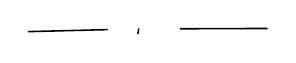
\begin{tikzpicture}[x=1cm,y=1cm,line width=.57pt,line cap=round]
\draw (0,0)--(1.00,.025) (1.39,-.025)--(1.40,.035) (1.93,.036)--(3.03,.04);
\end{tikzpicture}}\endgroup}
\end{GelfandAdjacentEvidence}
\begin{GelfandAdjacentEvidence}{GELFAND-P000842}{6}


Возникла группа \(SO(8)\), что-то было не так.

Франц. группа: [Зачёркнуто: \sout{…}\,\((8)\)] симметрия \(E_7\) и
\Incomplete{GELFAND-P000842}{french-group-cancellation}{Перед различимым «(8)» зачёркнутые буквы не читаются уверенно.}
\end{GelfandAdjacentEvidence}
\begin{GelfandAdjacentEvidence}{GELFAND-P000842}{7}

\[
\underline{E_7\longrightarrow SU(8)}
\]

тогда \uwave{расш. супергравитация}

\[
\dim E_7=133
\]

(\(E_7\) — комп. группа Ли)
\Unclear{GELFAND-P000842}{exceptional-group-note}{Сокращение перед «группа Ли» предварительно прочитано «комп.».}
\end{GelfandAdjacentEvidence}
\begin{GelfandAdjacentEvidence}{GELFAND-P000842}{8}


\uwave{Интересно}

[Зачёркнуто: \sout{…}] \uwave{сделать супертеорему об индексе}
\Incomplete{GELFAND-P000842}{index-theorem-cancelled-mark}{Перед «сделать» заштрихован знак. Исходное начертание неразличимо.}
\end{GelfandAdjacentEvidence}
\begin{GelfandAdjacentEvidence}{GELFAND-P000842}{9}


\uwave{Замечания}:

\(F_4\)

[Вставлено над строкой:] Эрмитовы

[Зачёркнуто: \sout{…}] \uwave{матрицы 3-го пор. из октав}; в них строится йорданово слож..
\Incomplete{GELFAND-P000842}{f4-cancellation}{Перед «матрицы» зачёркнута запись. Над ней вставлено «Эрмитовы».}
\end{GelfandAdjacentEvidence}
\begin{GelfandAdjacentEvidence}{GELFAND-P000842}{10}

\Unclear{GELFAND-P000842}{jordan-abbreviation}{Последнее сокращение предварительно прочитано «слож.».}
\end{GelfandAdjacentEvidence}
\begin{GelfandAdjacentEvidence}{GELFAND-P000842}{11}


произведение \(\frac12(AB+BA)\).

надо взять группу автоморфизмов этой йорд. алгебры; получим \(F_4\)

\uwave{Черн} — советник кит. президента — раб. в \uwave{Чикаго}.

\uwave{Янг} чит. лекции в Китае перед тысячной ауд.

\uline{И. М. Г.} — \uwave{что физики говорили} об Эйнштейне.

а) Э. и Н. Бор — самые крупные физ. в столетии

б) Э. в молодости сделал прекр. раб., но потом 30–40 лет заним. ерундой (пыт. созд. единую теорию поля).

в) \uwave{Э. — Борну}: „Хочу пригл. тебя в Принстон, но с такой старой клячей, [Вставлено над строкой: как я,] здесь всерьёз никто не считается“.
\Unclear{GELFAND-P000842}{einstein-quote-end}{Конец цитаты прочитан «никто не считается». Косая помета ведёт к вставке «как я».}
\end{GelfandAdjacentEvidence}
\begin{GelfandAdjacentEvidence}{GELFAND-P000842}{12}


[На левом поле:] \uuline{Доска}.
\Unclear{GELFAND-P000842}{margin-label}{Последняя буква предварительно прочитана «а».}
\end{GelfandAdjacentEvidence}
\begin{GelfandAdjacentEvidence}{GELFAND-P000842}{13}


\SourceFigure{GELFAND-P000842}{leaf-branch-diagram}{%
\begingroup\color{black}\GelfandFitDiagram{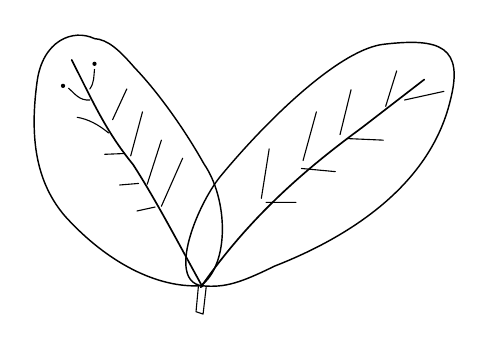
\begin{tikzpicture}[x=.010cm,y=-.010cm,line cap=round,line join=round]
\draw[line width=.52pt] (232,331) .. controls (178,334) and (114,303) .. (59,242)
 .. controls (27,204) and (13,153) .. (24,72)
 .. controls (31,19) and (70,4) .. (97,17)
 .. controls (114,18) and (129,32) .. (148,54)
 .. controls (175,82) and (209,128) .. (236,176)
 .. controls (267,221) and (269,304) .. (232,331);
\draw[line width=.52pt] (233,331) .. controls (189,324) and (227,229) .. (257,192)
 .. controls (319,117) and (411,29) .. (466,24)
 .. controls (536,16) and (567,27) .. (549,96)
 .. controls (522,208) and (413,272) .. (326,306)
 .. controls (283,327) and (263,334) .. (233,331);
\draw[semithick] (234,332) .. controls (202,274) and (175,222) .. (146,177)
 .. controls (111,134) and (95,97) .. (68,44);
\draw[semithick] (232,333) .. controls (297,239) and (373,177) .. (437,130)
 --(516,69);
\draw (91,81) .. controls (97,73) and (96,64) .. (97,56)
 (91,95) .. controls (78,96) and (72,87) .. (64,80)
 (115,137) .. controls (102,126) and (88,119) .. (75,117)
 (120,120)--(138,81)
 (143,166)--(158,110)
 (135,163)--(110,164)
 (164,202)--(182,146)
 (153,201)--(129,203)
 (182,230)--(209,169)
 (174,231)--(151,236);
\fill (97,49) circle[radius=2.7];
\fill (57,77) circle[radius=2.7];
\draw (309,220)--(319,157) (362,172)--(379,110)
 (409,139)--(423,82) (467,103)--(481,58)
 (315,225)--(353,225) (360,182)--(403,186)
 (418,144)--(464,146) (491,95)--(541,84);
\draw (229,332)--(226,364)--(235,367)--(239,332);
\end{tikzpicture}}\endgroup\par
Два контура сходятся у основания. На правой стороне некоторые короткие ветви отделены от основной линии.}
\end{GelfandAdjacentEvidence}
\begin{GelfandAdjacentEvidence}{GELFAND-P000842}{14}


\uwave{связь теор. физики с математикой}:

в фунд. вещах

(рисунок Янга)

\SourceFigure{GELFAND-P000842}{lower-right-hatching}{%
\begingroup\color{black}\GelfandFitDiagram{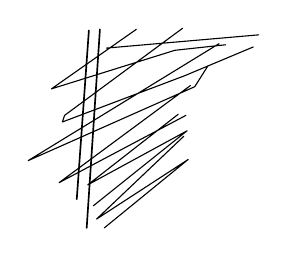
\begin{tikzpicture}[x=.014cm,y=-.014cm,line cap=round,line join=round]
\draw[semithick] (65,28)--(54,181) (75,27)--(63,207);
\draw (81,44)--(219,32)
 (108,27)--(31,81)--(143,46)--(189,41)
 (150,26)--(43,105)--(41,111)--(152,69)--(214,43)
 (183,40)--(10,146)--(161,79)--(173,60)
 (157,78)--(38,166)--(153,105)
 (146,104)--(64,168)--(154,119)--(69,187)
 (151,124)--(72,199)--(155,145)--(79,207);
\end{tikzpicture}}\endgroup\par
Почти вертикальные линии и наклонная штриховка. Отношение к левому рисунку неясно.}
\end{GelfandAdjacentEvidence}



\Needspace{7\baselineskip}
\begin{GelfandAdjacentEvidence}{GELFAND-P000843}{1}
\SourcePage{GELFAND-P000843}{unlabelled}
\uline{В. Е. Захаров.}

\SourceFigure{GELFAND-P000843}{reading-list-bracket}{%
\begingroup\color{black}\GelfandFitDiagram{\begin{tikzpicture}[x=1cm,y=1cm,every node/.style={font=\small,inner sep=1pt}]
\draw[semithick] (.34,.35)--(0,.35)--(0,-2.21)--(.35,-2.21);
\node[anchor=west] at (2.04,.12) {\uline{об ОТО читать:}};
\node[anchor=west] at (.55,-.49) {Дирак;};
\node[anchor=west] at (2.04,-.49) {Ландау, Лифшиц;};
\node[anchor=west] at (2.33,-1.05) {Вайнберг;};
\node[anchor=west] at (2.33,-1.58) {Хокинг, Эллис;};
\end{tikzpicture}}\endgroup\par
На правом поле. Левая скобка объединяет список.}
\end{GelfandAdjacentEvidence}
\begin{GelfandAdjacentEvidence}{GELFAND-P000843}{2}


\uwave{Математич. задача}:

\[
k=(k_1,\ldots,k_N)
\]

Рассм. ф-ю \(\omega(k)\) (вещественную) и пр-во пар \((k_1,k_2)\) размерности \(2N\) и там ур-е
\Unclear{GELFAND-P000843}{intro-short-word}{Короткое слово предварительно прочитано «там».}
\end{GelfandAdjacentEvidence}
\begin{GelfandAdjacentEvidence}{GELFAND-P000843}{3}


\begin{equation*}
\omega(k_1+k_2)=\omega(k_1)+\omega(k_2)
\tag{1}
\end{equation*}

\(\omega\) — нелин. \(\Rightarrow\) получ. поверхность \(\Gamma\) в \(R^{2n}\).

Сущ. ли другая ф-я \(f\), удовл. тому же ур-ю на \(\Gamma\):
\[
f(k_1+k_2)=f(k_1)+f(k_2)
\]
и не отлич. от \(\omega\) на линейную?
\Unclear{GELFAND-P000843}{linear-difference-verb}{Сокращённый глагол после «не» предварительно прочитан «отлич.».}
\end{GelfandAdjacentEvidence}
\begin{GelfandAdjacentEvidence}{GELFAND-P000843}{4}


[Зачёркнуто: \sout{Это}]
\Unclear{GELFAND-P000843}{cancel-before-situation}{Зачёркнутое слово предварительно прочитано «Это».}
\end{GelfandAdjacentEvidence}
\begin{GelfandAdjacentEvidence}{GELFAND-P000843}{5}

Эта сит. исключительна, т. к. размерность большая.

Идея Зах. и Шульмана:

как получать все ур-я, имеющие беск. число 1-х интегралов.

\uline{Пример}: \quad \uline{\(N=2\)}.

Задавать будем с пом. параметризации, \(\vec{k}=(p,q)\);

[Под строкой мелко:] в неявном виде \(\omega\) зад. так:
\Unclear{GELFAND-P000843}{example-small-word}{Мелкие слова предварительно прочитаны «в неявном виде».}
\end{GelfandAdjacentEvidence}
\begin{GelfandAdjacentEvidence}{GELFAND-P000843}{6}


\begin{equation*}
\omega(p,q),\qquad
\left[
\begin{aligned}
p&=\xi_1-\xi_2\\
q&=a(\xi_1)-a(\xi_2)\\
\omega&=b(\xi_1)-b(\xi_2)
\end{aligned}
\right.
\tag{2}
\end{equation*}

Другая [Зачёркнуто: \sout{…}] ф-я \(f\):
\Incomplete{GELFAND-P000843}{cancelled-other-function}{Короткая запись перед «ф-я» зачёркнута. Целое слово не читается.}
\end{GelfandAdjacentEvidence}
\begin{GelfandAdjacentEvidence}{GELFAND-P000843}{7}


\begin{equation*}
\left[
\begin{aligned}
p&=\xi_1-\xi_2\\
q&=a(\xi_1)-a(\xi_2)\\
f&=c(\xi_1)-c(\xi_2)
\end{aligned}
\right.
\qquad c\text{ — другая ф-я (любая)}
\tag{3}
\end{equation*}
\Unclear{GELFAND-P000843}{third-system-rewritten}{Предварительно набрано \(f=c(\xi_1)-c(\xi_2)\). Левая буква похожа на \(\varphi\), а первая справа на \(e\).}
\end{GelfandAdjacentEvidence}
\begin{GelfandAdjacentEvidence}{GELFAND-P000843}{8}


Вопрос: явл. ли это общей конструкцией?

Идея: параметризацию \(\Gamma\) зададим (она 3-мерна)
\Unclear{GELFAND-P000843}{parametrization-pronoun}{Окончания предварительно прочитаны «она 3-мерна».}
\end{GelfandAdjacentEvidence}
\begin{GelfandAdjacentEvidence}{GELFAND-P000843}{9}


\begin{equation*}
\begin{cases}
p_1=\xi_1-\xi_2\\
q_1=a(\xi_1)-a(\xi_2)\\
p_2=\xi_2-\xi_3\\
q_2=a(\xi_2)-a(\xi_3)
\end{cases}
\tag{4}
\end{equation*}

\[
\underbrace{p_1+p_2}_{p_3}\qquad
\underbrace{q_1+q_2}_{q_3}\qquad
p_3=\xi_1-\xi_3
\]

и т. д.
\Unclear{GELFAND-P000843}{bottom-connector}{Первый знак предварительно прочитан «и».}
\end{GelfandAdjacentEvidence}



\Needspace{7\baselineskip}
\begin{GelfandAdjacentEvidence}{GELFAND-P000844}{1}
\SourcePage{GELFAND-P000844}{67}
[Над первой строкой зачёркнуто: \sout{…}]
\Incomplete{GELFAND-P000844}{top-cancelled}{Над первой строкой короткая запись затушёвана. Её буквы неразличимы.}
\end{GelfandAdjacentEvidence}
\begin{GelfandAdjacentEvidence}{GELFAND-P000844}{2}


Отсюда если вырождена, то серьёзно (функц. параметр).
\Unclear{GELFAND-P000844}{opening-condition}{Короткое слово предварительно прочитано «если».}
\end{GelfandAdjacentEvidence}
\begin{GelfandAdjacentEvidence}{GELFAND-P000844}{3}


Сущ. метод констр. систем с предст. Лакса (Захаров-Шабат)
\begin{equation*}
\frac{\partial L}{\partial t}-\frac{\partial A}{\partial y}+[L,A]=0
\tag{5}
\end{equation*}

\[
\begin{aligned}
L&=\frac{\partial^n}{\partial x^n}+\ldots\\
A&=\frac{\partial^m}{\partial x^m}+\ldots
\end{aligned}
\]

(5) — нелин. сист. ур-й на коэфф.

Рассм. её \uline{линеаризацию}.
\SourceFigure{GELFAND-P000844}{linearization-connector}{%
\begingroup\color{black}\GelfandFitDiagram{\begin{tikzpicture}[x=1cm,y=1cm,every node/.style={font=\small,inner sep=1pt}]
\node[anchor=west] at (0,0) {\uline{линеаризацию}.};
\node[anchor=west] at (3.05,0) {Это};
\node[anchor=west] at (.42,-.77) {(отбросим нелин. члены)};
\draw (3.05,.12) .. controls (3.05,-.25) and (3.74,-.28) .. (4.06,-.30)
 .. controls (4.51,-.35) and (5.19,-.37) .. (5.25,-.70);
\end{tikzpicture}}\endgroup\par
Приписка под строкой. Соединяющая черта подходит к слову «Это».}
\end{GelfandAdjacentEvidence}
\begin{GelfandAdjacentEvidence}{GELFAND-P000844}{4}


Это сист. с пост. коэфф., она реш. методом Фурье.

\[
u_j\sim\exp(-\omega t+qy+px)
\]
\[
\omega=\omega(p,q)
\]

Те сист. выглядят так как в
\Unclear{GELFAND-P000844}{systems-phrase-start}{Начальное слово предварительно прочитано «Те».}
\end{GelfandAdjacentEvidence}
\begin{GelfandAdjacentEvidence}{GELFAND-P000844}{5}

\Unclear{GELFAND-P000844}{systems-phrase-final}{После «как» стоит отдельное «в». Фраза обрывается перед обозначениями.}
\end{GelfandAdjacentEvidence}
\begin{GelfandAdjacentEvidence}{GELFAND-P000844}{6}


\(a(\xi)\) — символ опер. \(L\)

\(b(\xi)\) — ″ — \(A\)

[На правом поле:]
\SourceFigure{GELFAND-P000844}{side-note-separator}{%
\begingroup\color{black}\GelfandFitDiagram{\begin{tikzpicture}[x=1cm,y=1cm,every node/.style={inner sep=1pt}]
\draw (.22,.68)..controls (.25,.27) and (.17,-.19)..(.08,-.72);
\draw (.35,.66)..controls (.37,.25) and (.28,-.29)..(.23,-.81);
\node[anchor=west] at (.67,.19)
 {\(\begin{aligned}L&=L_0+\delta L\\ A&=A_0+\delta A\end{aligned}\)};
\end{tikzpicture}}\endgroup}
\end{GelfandAdjacentEvidence}
\begin{GelfandAdjacentEvidence}{GELFAND-P000844}{7}

\(\delta L,\delta A\) — всё, что содержит переменные коэфф.

Вырожд. законы дисп. связаны с обр. задачей.

\[
\begin{aligned}
p&=\xi_1-\xi_2\\
q&=\ell(\xi_1)-\ell(\xi_2)\\
\omega&=a(\xi_1)-a(\xi_2)
\end{aligned}
\]
\(a,\ell\) — симв. \(A_0,L_0\).

Рассм. ур-е Г.-Л.-М.:
\[
F+K+K\oplus F=0
\]
\Unclear{GELFAND-P000844}{circled-plus}{Между \(K\) и \(F\) виден плюс в круге.}
\end{GelfandAdjacentEvidence}
\begin{GelfandAdjacentEvidence}{GELFAND-P000844}{8}


\[
\begin{aligned}
\frac{\partial F}{\partial t}+[L_0,F]&=0\\
\frac{\partial F}{\partial y}+[A_0,F]&=0
\end{aligned}
\]
\Unclear{GELFAND-P000844}{retraced-derivative-plus}{Во второй строке плюс переправлен, но виден.}
\end{GelfandAdjacentEvidence}
\begin{GelfandAdjacentEvidence}{GELFAND-P000844}{9}


\[
K=-F
\]
\[
F=\exp\bigl(\xi_1x-\xi_2z+[\ell(\xi_1)-\ell(\xi_2)]y+[a(\xi_1)-a(\xi_2)]t\bigr)
\]
\Unclear{GELFAND-P000844}{exponential-overwritten-coordinate}{Буква после \(\xi_2\) густо переписана. Предварительно прочитано \(z\).}
\end{GelfandAdjacentEvidence}
\begin{GelfandAdjacentEvidence}{GELFAND-P000844}{10}


Здесь связь уст., когда \(\ell\) и \(a\) — полиномы; можно уст. связь для рац. функций.
\Unclear{GELFAND-P000844}{retrace-ell}{Буква \(\ell\) перед «и» переправлена.}
\end{GelfandAdjacentEvidence}
\begin{GelfandAdjacentEvidence}{GELFAND-P000844}{11}


\SourceFigure{GELFAND-P000844}{polynomial-bracket}{%
\begingroup\color{black}\GelfandFitDiagram{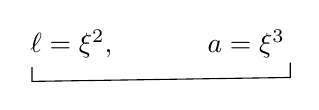
\begin{tikzpicture}[x=1cm,y=1cm,every node/.style={inner sep=1pt}]
\node at (.50,.25) {\(\ell=\xi^2,\)};
\node at (2.72,.25) {\(a=\xi^3\)};
\draw (0,-.04)--(0,-.22)--(3.28,-.17)--(3.28,.02);
\end{tikzpicture}}\endgroup}
\end{GelfandAdjacentEvidence}
\begin{GelfandAdjacentEvidence}{GELFAND-P000844}{12}


\(L,A\) ищутся — получ. KdV.
\Unclear{GELFAND-P000844}{final-verb}{Глагол предварительно прочитан «ищутся».}
\end{GelfandAdjacentEvidence}



\Needspace{7\baselineskip}
\begin{GelfandAdjacentEvidence}{GELFAND-P000845}{1}
\SourcePage{GELFAND-P000845}{unlabelled}
Интегр. обр. задачи \(\Rightarrow\) закон дисп. вырожден.

\SourceFigure{GELFAND-P000845}{divider-first}{%
\begingroup\color{black}\GelfandFitDiagram{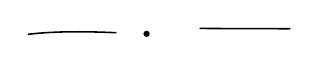
\begin{tikzpicture}[x=1cm,y=1cm,line width=.56pt,line cap=round]
\draw (0,-.02) .. controls (.36,.025) and (.82,.013) .. (1.11,0)
 (2.18,.054)--(3.32,.05);
\fill (1.50,-.014) circle[radius=.04cm];
\end{tikzpicture}}\endgroup}
\end{GelfandAdjacentEvidence}
\begin{GelfandAdjacentEvidence}{GELFAND-P000845}{2}


Матрицы \(L\) и \(A\): уже не обязательно

[На левом поле:] \uline{Альтерн.}
\Unclear{GELFAND-P000845}{margin-alternative}{Подчёркнутое слово на поле предварительно прочитано «Альтерн.».}
\end{GelfandAdjacentEvidence}
\begin{GelfandAdjacentEvidence}{GELFAND-P000845}{3}


Если ур-е интегр., а закон дисп. невыр., то взаимод. \(\equiv 0\) на мн-зии.
\Unclear{GELFAND-P000845}{resonance-abbreviation}{Конечное сокращение предварительно прочитано «мн-зии».}
\end{GelfandAdjacentEvidence}
\begin{GelfandAdjacentEvidence}{GELFAND-P000845}{4}


\SourceFigure{GELFAND-P000845}{divider-second}{%
\begingroup\color{black}\GelfandFitDiagram{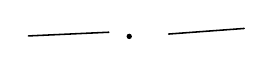
\begin{tikzpicture}[x=1cm,y=1cm,line width=.56pt,line cap=round]
\draw (0,-.04)--(1.02,.007) (1.78,-.016)--(2.74,.055);
\fill (1.28,-.046) circle[radius=.034cm];
\end{tikzpicture}}\endgroup}
\end{GelfandAdjacentEvidence}
\begin{GelfandAdjacentEvidence}{GELFAND-P000845}{5}


\[
\omega=\frac18\bigl[(p+\tfrac qp)^3-(-p+\tfrac qp)^3
=\frac14\bigl[p^3+\tfrac{3q^2}{p}\bigr]
\]
\Unclear{GELFAND-P000845}{dispersion-bracket}{Перед вторым знаком равенства закрывающая квадратная скобка не видна.}
\end{GelfandAdjacentEvidence}
\begin{GelfandAdjacentEvidence}{GELFAND-P000845}{6}


\uwave{Ур-е Кад.-Петв.}:
\[
u_t\overset{?}{+}\frac14
\left(u_{xxx}+6uu_x-3\int_{-\infty}^{x}u_{yy}\,dx\right)
\]
\Unclear{GELFAND-P000845}{kp-relation}{Вертикальный штрих пересекает два горизонтальных. Предварительно набран плюс. Первоначальный знак неясен.}
\end{GelfandAdjacentEvidence}
\begin{GelfandAdjacentEvidence}{GELFAND-P000845}{7}


выше выписал её символ.
\Unclear{GELFAND-P000845}{kp-note}{Глагол предварительно прочитан «выписал». Возможно «выписан».}
\end{GelfandAdjacentEvidence}
\begin{GelfandAdjacentEvidence}{GELFAND-P000845}{8}


\(\xi^2\) и \(\xi^3\) одеваем — получ. К.-П.-ур-е.

Т. е. К.-П. обладает именно этим зак. дисп. (как в примере)

\SourceFigure{GELFAND-P000845}{divider-third}{%
\begingroup\color{black}\GelfandFitDiagram{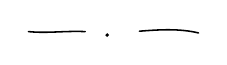
\begin{tikzpicture}[x=1cm,y=1cm,line width=.56pt,line cap=round]
\draw (0,0) .. controls (.24,-.024) and (.45,.011) .. (.72,0)
 (1.41,.005) .. controls (1.67,.026) and (1.92,.04) .. (2.16,-.017);
\fill (1.00,-.044) circle[radius=.025cm];
\end{tikzpicture}}\endgroup}
\end{GelfandAdjacentEvidence}
\begin{GelfandAdjacentEvidence}{GELFAND-P000845}{9}


\uwave{Эксперим. факт.}: одеваем пару
\[
L_0=\begin{bmatrix}1&0\\0&-1\end{bmatrix}\frac{\partial}{\partial x},
\qquad
A_0=\begin{bmatrix}1&0\\0&1\end{bmatrix}\frac{\partial^2}{\partial x^2}
\]
Получим
\[
L=\begin{bmatrix}1&0\\0&-1\end{bmatrix}\frac{\partial}{\partial x}
+\begin{bmatrix}0&\psi\\\bar\psi&0\end{bmatrix}
\]
и ур-е
\begin{equation*}
\left\{\begin{aligned}
i\frac{\partial\psi}{\partial t}-\frac{\partial^2\psi}{\partial x^2}
+\frac{\partial^2\psi}{\partial y^2}+u\psi&=0\\
\left(\frac{\partial^2}{\partial x^2}+\frac{\partial^2}{\partial y^2}\right)u
&=\left(\frac{\partial^2}{\partial x^2}-\frac{\partial^2}{\partial y^2}\right)|\psi|^2
\end{aligned}\right.
\tag{6}
\end{equation*}
сист. Д… — Стюартсона (см. гидродин., теор. пов. волн)
\Unclear{GELFAND-P000845}{system-name}{Первое имя начинается с «Д». Продолжение не читается уверенно.}
\end{GelfandAdjacentEvidence}
\begin{GelfandAdjacentEvidence}{GELFAND-P000845}{10}


Возьмём преобр. Фурье. Получим сист. вида:
\[
\psi\to a(k)
\]
\[
i\frac{\partial a(k)}{\partial t}=\frac{\delta H}{\delta a(k)}
\]
\Unclear{GELFAND-P000845}{variational-denominator}{Над \(a(k)\) в знаменателе вариационной производной черта не видна.}
\end{GelfandAdjacentEvidence}
\begin{GelfandAdjacentEvidence}{GELFAND-P000845}{11}


\[
\begin{aligned}
H={}&\int\omega_k|a_k|^2\,dk\\
&+\int w^{[\Gamma]}_{kk_1k_2k_3}
\bar a_k\bar a_{k_1}a_{k_2}a_{k_3}
\delta_{k+k_1-k_2-k_3}\,dk_2\,dk_3
\end{aligned}
\]
\Unclear{GELFAND-P000845}{hamiltonian-coefficient}{Коэффициент предварительно прочитан \(w\). Справа вверху отдельный штрих, похожий на \(\Gamma\).}
\end{GelfandAdjacentEvidence}
\begin{GelfandAdjacentEvidence}{GELFAND-P000845}{12}

\Unclear{GELFAND-P000845}{hamiltonian-measure}{У края кадра видны два дифференциала. Первый индекс предварительно прочитан \(2\).}
\end{GelfandAdjacentEvidence}
\begin{GelfandAdjacentEvidence}{GELFAND-P000845}{13}


\[
w=\frac{(p_1-p_3)^2-(q_1-q_3)^2}{(p_1-p_3)^2+(q_1-q_3)^2}
+\frac{(p_2-p_4)^2-(q_2-q_4)^2}{(p_2+p_4)^2+(q_2+q_4)^2}
\]
\Unclear{GELFAND-P000845}{bottom-first-q}{Индекс у первого \(q\) в обеих строках первой дроби предварительно прочитан \(1\).}
\end{GelfandAdjacentEvidence}
\begin{GelfandAdjacentEvidence}{GELFAND-P000845}{14}

\Unclear{GELFAND-P000845}{bottom-denominator-signs}{Во втором знаменателе видны плюсы в обеих скобках.}
\end{GelfandAdjacentEvidence}



\Needspace{7\baselineskip}
\begin{GelfandAdjacentEvidence}{GELFAND-P000846}{1}
\SourcePage{GELFAND-P000846}{68}
В пр-ве \(k_1,k_2,k_3,k_4\)
\Unclear{GELFAND-P000846}{fourth-wave-vector}{Буква при индексе \(4\) переправлена. Предварительно набрано \(k_4\).}
\end{GelfandAdjacentEvidence}
\begin{GelfandAdjacentEvidence}{GELFAND-P000846}{2}


рассм. ур-е
\[
\begin{gathered}
\omega(k_1)+\omega(k_2)=\omega(k_3)+\omega(k_4);\\
k_1+k_2=k_3+k_4
\end{gathered}
\]
[Зачёркнуто: \sout{…}]
\Incomplete{GELFAND-P000846}{cancelled-top-line}{Под равенствами короткая запись и длинная строка густо зачёркнуты. Текст не читается.}
\end{GelfandAdjacentEvidence}
\begin{GelfandAdjacentEvidence}{GELFAND-P000846}{3}


Оказ., что \(w|_\Gamma=0\).

\uline{Гип. Арнольда}: Это теор. Пуанкаре \uwave{об интегрируемости}. (когда есть 1-й инт., незав. от эн.)

Усл. Пуанкаре: ампл. рез. гармоник должны быть \(0\)

(см. Пуанкаре, неб. мех., или Арнольд: доп. главы)

\uwave{Пуанкаре}: гамильтониан
\[
H=H_0(p)+\varepsilon\sum h_k(p)e^{ikq}
\]

\(p=I,\quad q=\psi\).
\Unclear{GELFAND-P000846}{angle-symbol}{Угловой знак предварительно прочитан \(\psi\). Возможно \(\varphi\).}
\end{GelfandAdjacentEvidence}
\begin{GelfandAdjacentEvidence}{GELFAND-P000846}{4}


Когда \(\exists\) инт. \(F(p,q,\varepsilon)\) (всё периодично по \(q\)),

[Под \(F\):] незав. от \(H\).

\uwave{Необх. условие}: составим \(\lambda=\frac{\partial H_0}{\partial p}\) и наложим на неё усл. невыр.
\Unclear{GELFAND-P000846}{nondegeneracy-lambda}{Знак слева от производной густо переправлен. Предварительно набрано \(\lambda\).}
\end{GelfandAdjacentEvidence}
\begin{GelfandAdjacentEvidence}{GELFAND-P000846}{5}


\[
\det\left|\frac{\partial\lambda}{\partial p}\right|\ne0
\]
\Unclear{GELFAND-P000846}{determinant-lambda}{Знак в числителе производной также переправлен. Предварительно набрано \(\lambda\).}
\end{GelfandAdjacentEvidence}
\begin{GelfandAdjacentEvidence}{GELFAND-P000846}{6}

— одно из усл. невыр. (всего их 2)

Интегралов нет, если
\[
\Gamma:\quad\langle k,\lambda(p)\rangle=0
\]
\Unclear{GELFAND-P000846}{resonance-lambda}{Знак перед \((p)\) переправлен. Предварительно набрано \(\lambda\).}
\end{GelfandAdjacentEvidence}
\begin{GelfandAdjacentEvidence}{GELFAND-P000846}{7}


Усл. Пуанкаре:
\[
\underline{h_k|_{\Gamma_k}=0},\qquad k\in\mathbb Z^n.
\]
если оно наруш. беск. число раз, то интеграла нет

Идея: \(\lambda\leftrightarrow\omega\).

\uline{Арн.} \quad ф-лы (2) означают, что есть \uwave{пов. переноса}.

\SourceFigure{GELFAND-P000846}{diagram-01}{%
\begingroup\color{black}\GelfandFitDiagram{\begin{tikzpicture}[x=.013cm,y=-.013cm,line cap=round,line width=.60pt]
\draw (11,163) .. controls (44,156) and (99,128) .. (135,89)
 .. controls (149,73) and (166,43) .. (171,26);
\draw[semithick] (60,145) .. controls (79,158) and (99,210) .. (102,262);
\draw[semithick] (58,154) .. controls (48,148) and (57,129) .. (65,134)
 .. controls (74,140) and (66,153) .. (58,154);
\end{tikzpicture}}\endgroup\par
Кривые сходятся у небольшой петли. Утолщение слева и петля переданы по очертаниям. Стрелки не различимы уверенно.}
\end{GelfandAdjacentEvidence}
\begin{GelfandAdjacentEvidence}{GELFAND-P000846}{8}


двигаем 2-ю кривую по 1-й,

параллельно перенося её

\uline{Кривые}:
\[
\begin{aligned}
p&=\xi_1; &\qquad p&=-\xi_2\\
q&=a(\xi_1); &q&=-a(\xi_2)\\
\omega&=b(\xi_1); &\omega&=-b(\xi_2)
\end{aligned}
\]

Кривая двиг. сама по себе.

\uuline{Захаров}.
\[
\omega_1(k_1+k_2)=\omega_2(k_1)+\omega_3(k_2)
\]
получ. общие пов. переноса.

\SourceFigure{GELFAND-P000846}{transfer-divider}{%
\begingroup\color{black}\GelfandFitDiagram{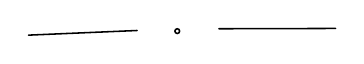
\begin{tikzpicture}[x=1cm,y=1cm,line cap=round,line width=.56pt]
\draw (0,0)--(1.38,.059) (2.42,.081)--(3.90,.085);
\draw (1.89,.051) circle[radius=.030cm];
\end{tikzpicture}}\endgroup}
\end{GelfandAdjacentEvidence}
\begin{GelfandAdjacentEvidence}{GELFAND-P000846}{9}


\uwave{Рецепт действий}. Проверяем, вырожд. ли закон дисп.; затем смотрим.

\(0\) или не \(0\) там гам. взаимод.
\Unclear{GELFAND-P000846}{final-coefficient}{Сокращение перед «взаимод.» предварительно прочитано «гам.».}
\end{GelfandAdjacentEvidence}


Что если интегралы начин. сразу с высших порядков?


\Needspace{7\baselineskip}
\begin{GelfandAdjacentEvidence}{GELFAND-P000847}{1}
\SourcePage{GELFAND-P000847}{unlabelled}
\uuline{Арн.} \quad \uwave{биркгоф}.
\Unclear{GELFAND-P000847}{first-birkhoff}{Первая помета читается «Арн.». В следующем слове неясна точка.}
\end{GelfandAdjacentEvidence}
\begin{GelfandAdjacentEvidence}{GELFAND-P000847}{2}


\[
H=\sum\omega_k z_k\bar z_k+\ldots
\]

[зачёркнуто: \sout{\(H=\)}]
\Unclear{GELFAND-P000847}{cancelled-h}{Под штрихами читается \(H\). После него, возможно, знак равенства.}
\end{GelfandAdjacentEvidence}
\begin{GelfandAdjacentEvidence}{GELFAND-P000847}{3}

\[
\sum\omega_k(p_k^2+q_k^2)+\ldots
\]

[Справа:]
\[
z=p+iq,\qquad \Pi_k=z_k\bar z_k
\]

биркгоф: \uwave{в нерез. случае прив. к \(H(\Pi_k)\)}.
\Unclear{GELFAND-P000847}{nonresonant-abbreviation}{Сокращение после «случае» предварительно прочитано «прив.».}
\end{GelfandAdjacentEvidence}
\begin{GelfandAdjacentEvidence}{GELFAND-P000847}{4}


(если \(\omega_k\) независимы)

[Справа:] (на уровне форм. рядов)

\uline{И. М. Г.} \quad \uwave{Краткий список того, что надо знать}.

1. \uwave{Соврем. абстр. язык} \quad (см. напр., 1-ю часть кн. \uline{Кириллова})
\SourceFigure{GELFAND-P000847}{glossary-arrow}{%
\begingroup\color{black}\GelfandFitDiagram{\begin{tikzpicture}[x=.008cm,y=-.008cm,line width=.55pt,every node/.style={inner sep=1pt}]
\draw (31,47)--(268,44)--(265,150)--(747,155);
\draw[->] (389,17)--(388,63);
\node at (393,105) {\uwave{словарь}};
\end{tikzpicture}}\endgroup\par
Под ссылкой ступенчатая черта и стрелка к слову «словарь».}
\end{GelfandAdjacentEvidence}
\begin{GelfandAdjacentEvidence}{GELFAND-P000847}{5}


2. \uline{Арнольд}: дифф. ур. \(+\) доп. главы

(чтобы привыкнуть к анализу)

3. \uwave{По алгебре}: 2 главы кн. \uline{Серра} по
[зачёркнуто: \sout{представлениям}] предст. кон. групп.
\Unclear{GELFAND-P000847}{algebra-cancelled}{Зачёркнутое слово предварительно прочитано «представлениям».}
\end{GelfandAdjacentEvidence}
\begin{GelfandAdjacentEvidence}{GELFAND-P000847}{6}


[Над строкой зачёркнуто: \sout{все}]
\Unclear{GELFAND-P000847}{all-cancelled}{Зачёркнутое слово предварительно прочитано «все».}
\end{GelfandAdjacentEvidence}
\begin{GelfandAdjacentEvidence}{GELFAND-P000847}{7}


все кроме \uwave{1 гл.} кн. \uline{Серра} по гр. и алг. Ли
(особенно, посл. главу)

[Над строкой зачёркнуто: \sout{…}]
\Incomplete{GELFAND-P000847}{linear-cancelled}{Короткое слово над «Лин. алгебра» зачёркнуто. Оно не читается.}
\end{GelfandAdjacentEvidence}
\begin{GelfandAdjacentEvidence}{GELFAND-P000847}{8}


\uwave{Лин. алгебра}: Гельфанд; Мальцев

4. \uwave{Дифф. геометрию} в 2-х вар.: старый тензорный
(см. \uline{Дирак} о теории отн.; и \uline{Ландау и Лифшиц})
\Unclear{GELFAND-P000847}{old-tensor-otn}{Сокращение после «теории» предварительно прочитано «отн.».}
\end{GelfandAdjacentEvidence}


совр. вар.: векторные рассл. и связности.

5. \uwave{Представления}: Г. Вейль

лекции Рака \quad Racah.

Гельфанд, Минлос, Шапиро


\clearpage
\pdfbookmark[0]{Глава 16}{gelfand-archive-chapter-16}
\section*{Глава 16}


\Needspace{7\baselineskip}
\begin{GelfandAdjacentEvidence}{GELFAND-P000848}{1}
\SourcePage{GELFAND-P000848}{1}
\uline{1.10.79} \qquad \uline{Сем. Гельфанда}
\Unclear{GELFAND-P000848}{date-header}{Месяц предварительно прочитан «10». Второй знак пропечатан не полностью.}
\end{GelfandAdjacentEvidence}
\begin{GelfandAdjacentEvidence}{GELFAND-P000848}{2}


[Зачёркнутый заголовок: \sout{КАЛЛОШ?}]
\Unclear{GELFAND-P000848}{top-cancelled-heading}{«КАЛЛОШ» — возможное чтение зачёркнутого заголовка.}
\end{GelfandAdjacentEvidence}
\begin{GelfandAdjacentEvidence}{GELFAND-P000848}{3}


\uline{И. М. Г.} Что такое спинор?

\uwave{Книга Паули по квант. мех.} — самое хорошее излож. теории Дирака (ур-е Дирака)
\Unclear{GELFAND-P000848}{book-abbreviation}{Переправленное сокращение предварительно прочитано «квант.».}
\end{GelfandAdjacentEvidence}
\begin{GelfandAdjacentEvidence}{GELFAND-P000848}{4}


Возражения его против теор. Дирака:

а) сущ. \uline{позитронов}, предсказ. теор. Дирака.

б) если они есть, то при столкн. с позитр. получ. 2 фотона
\Unclear{GELFAND-P000848}{annihilation-word}{Сокращение после «с» предварительно прочитано «позитр.».}
\end{GelfandAdjacentEvidence}
\begin{GelfandAdjacentEvidence}{GELFAND-P000848}{5}


в) 2 фотона по этой теории могут родить пару эл-н/позитрон
\Unclear{GELFAND-P000848}{pair-abbreviation}{Перед косой чертой предположительно «эл-н».}
\end{GelfandAdjacentEvidence}
\begin{GelfandAdjacentEvidence}{GELFAND-P000848}{6}


Дирак отказ., чтобы не сделали „сэром“ (?)
\Unclear{GELFAND-P000848}{dirac-abbreviation}{Сокращение после «Дирак» предварительно прочитано «отказ.».}
\end{GelfandAdjacentEvidence}
\begin{GelfandAdjacentEvidence}{GELFAND-P000848}{7}


[Строки объединены скобкой слева.]

Однажды ему кто-то сказал, что не понимает ф-лу в левом нижнем углу доски.

Дирак не отвечает.

Председатель просит его ответить

[Зачёркнуто: \sout{…}] Дирак: „не было вопроса, было утверждение“.
\Incomplete{GELFAND-P000848}{anecdote-cancelled-word}{Зачёркнутый фрагмент перед «Дирак» не читается.}
\end{GelfandAdjacentEvidence}
\begin{GelfandAdjacentEvidence}{GELFAND-P000848}{8}

\SourceFigure{GELFAND-P000848}{anecdote-bracket}{%
\begingroup\color{black}\GelfandFitDiagram{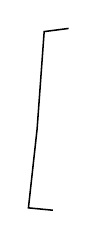
\begin{tikzpicture}[x=.01cm,y=-.01cm,line width=.55pt]
\draw (69,16)--(38,20)--(29,144)--(18,244)--(49,247);
\end{tikzpicture}}\endgroup\par
Скобка слева от четырёх предыдущих строк.}
\end{GelfandAdjacentEvidence}
\begin{GelfandAdjacentEvidence}{GELFAND-P000848}{9}


\uwave{Гамильтон}: хотел извлечь корень из \(x^2+y^2+z^2\), причем получить „лин. форму“
\[
-(x^2+y^2+z^2)=(ax+by+cz)^2
\]
\[
a^2=b^2=c^2=-1
\]
\Unclear{GELFAND-P000848}{hamilton-square-sign}{После \(c^2\) переправленный знак предварительно прочитан \(=-1\).}
\end{GelfandAdjacentEvidence}
\begin{GelfandAdjacentEvidence}{GELFAND-P000848}{10}

\[
\begin{aligned}
&(ab+ba)\,[?]\,xy+(ac+ca)xz+(bc+cb)yz\\
&\qquad{}+a^2x^2+b^2y^2+c^2z^2=-(x^2+y^2+z^2).
\end{aligned}
\]
\Unclear{GELFAND-P000848}{hamilton-factor-mark}{Между первой скобкой и \(xy\) находится неразобранный тёмный штрих.}
\end{GelfandAdjacentEvidence}
\begin{GelfandAdjacentEvidence}{GELFAND-P000848}{11}


отсюда соотношения
\[
ab+ba=0 \quad \text{и т. д.}
\]
Добавл. единицу — получ. \uwave{кватернионы}.

Рассм. преобразование
\[
z'=\frac{az+b}{cz+d}
\]

или
\[
\begin{cases}
z'_1=az_1+bz_2\\
z'_2=cz_1+dz_2
\end{cases}
\qquad z'=\frac{z'_1}{z'_2},\quad z=\frac{z_1}{z_2}.
\]

Спиноры — пара чисел [под словом «чисел»: (компл.)], преобр. по такому закону

Компл. сопр. — \uline{сопр.} \uline{спинор}.
\SourceFigure{GELFAND-P000848}{spinor-divider}{%
\begingroup\color{black}\GelfandFitDiagram{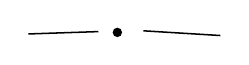
\begin{tikzpicture}[x=.01cm,y=-.01cm,line width=.55pt]
\draw (19,47)--(108,44);
\fill (132,45) circle[radius=1.7pt];
\draw (165,43)--(263,49);
\end{tikzpicture}}\endgroup\par
Две короткие черты с точкой посередине.}
\end{GelfandAdjacentEvidence}
\begin{GelfandAdjacentEvidence}{GELFAND-P000848}{12}


\uline{Гравитацию} надо читать по Ландау и Лифшицу (т. 2)

\uwave{гл. 1, 2, 10, 11.}

\uwave{Рената Э. Каллош.}

\uline{Программа.}

1. Двухкомпонентные спиноры.

2. Самодуальность.

3. Дифф. оператор \(\Delta(A,B)\), описыв. ур-е для частиц высш. спинов.

4. Ур-е теплопров., нулевые и ненулевые моды.

5. Теоремы об индексе.

6. Супертеор. в гравит. поле

7. Суперсамодуальность.

(8. Супертеор. об индексе! Ею занимается Зингер, но на самом деле её нет)
\Unclear{GELFAND-P000848}{program-last-number}{После раскрывающей скобки предполагается цифра 8.}
\end{GelfandAdjacentEvidence}
\begin{GelfandAdjacentEvidence}{GELFAND-P000848}{13}

\Unclear{GELFAND-P000848}{program-last-verb}{Начало фразы предварительно прочитано «Ею занимается».}
\end{GelfandAdjacentEvidence}



\Needspace{7\baselineskip}
\begin{GelfandAdjacentEvidence}{GELFAND-P000849}{1}
\SourcePage{GELFAND-P000849}{unlabelled}
\uline{Лит-ра}

1. [Зачёркнуто: \sout{…}] \uline{S. W. Hawking}, \uline{C. N. Pope}
\Incomplete{GELFAND-P000849}{bibliography-first-cancelled}{Перед «S. W. Hawking» зачёркнут короткий фрагмент. Он не читается.}
\end{GelfandAdjacentEvidence}
\begin{GelfandAdjacentEvidence}{GELFAND-P000849}{2}


Nucl. Phys., B 146 (1978), 381
\Unclear{GELFAND-P000849}{bibliography-first-year}{Последняя цифра года предварительно прочитана 8. По штрихам возможно 1.}
\end{GelfandAdjacentEvidence}
\begin{GelfandAdjacentEvidence}{GELFAND-P000849}{3}


2. \uline{Р. Э. Каллош}, Письма в ЖЭТФ,

\uline{29} (1979), 192; 493

3. S. M. Christensen, M. J. Duff.

Nucl. Phys. (1979), 301

4. — „ —, — „ — Deser, Gr[?]
\Unclear{GELFAND-P000849}{bibliography-fourth-last-author}{После «Deser» предварительно прочитано «Gr» с неясным окончанием. Первую букву можно принять за «C».}
\end{GelfandAdjacentEvidence}
\begin{GelfandAdjacentEvidence}{GELFAND-P000849}{4}


Phys Lett. \uline{84 B} (1979), 411

[1] — осн. вклад в супергравит. (в 1-петлевом прибл.) — от \(0^{\underline{\text{х}}}\) мод
\Unclear{GELFAND-P000849}{superscript-zero}{При нуле маленький надстрочный знак «х» с подчёркиванием.}
\end{GelfandAdjacentEvidence}
\begin{GelfandAdjacentEvidence}{GELFAND-P000849}{5}


(в Я.-М. — от всех мод!)

[2], [3] незав. — в суперграв. (для самодуальн.) для более высоких порядков

Перед этим было в 1-м и 2-м пор. суперг. не сод. расход.
\Unclear{GELFAND-P000849}{before-supergravity}{Слово предварительно прочитано «было». Последняя буква неясна.}
\end{GelfandAdjacentEvidence}
\begin{GelfandAdjacentEvidence}{GELFAND-P000849}{6}


[3] осн. на обычной теор. об индексе.

\uwave{2-комп. формализм Ван-дер-Вардена.}

\[
\Psi_\alpha\longrightarrow\Psi_\beta\Omega_\alpha^\beta \tag{1}
\]

[Справа:] Закон преобразований

\(\Psi_\alpha\in(\text{пр. станд. 2-мерн. пр. }SL(2,C))=V;\)
\Unclear{GELFAND-P000849}{margin-representation-abbreviation}{Первое сокращение предварительно прочитано «пр.». Возможна начальная «и».}
\end{GelfandAdjacentEvidence}
\begin{GelfandAdjacentEvidence}{GELFAND-P000849}{7}


\(\Psi_{\dot\alpha}\in\bar V\), \(V\otimes\bar V\) имеет вещ. стр.
и гр. \(SL(2,C)\) сохр. кв. форму.

(гр. напр. у Пенроуза)
\Unclear{GELFAND-P000849}{preserve-quadratic-form}{Сокращение в скобках предварительно прочитано «напр.».}
\end{GelfandAdjacentEvidence}
\begin{GelfandAdjacentEvidence}{GELFAND-P000849}{8}


\(SL(2,C)\) как вещ. мн. Ли
\Unclear{GELFAND-P000849}{margin-real-lie}{Сокращение после «вещ.» предварительно прочитано «мн.». Возможно «гр.».}
\end{GelfandAdjacentEvidence}
\begin{GelfandAdjacentEvidence}{GELFAND-P000849}{9}

\SourceFigure{GELFAND-P000849}{margin-stepped-bracket}{%
\begingroup\color{black}\GelfandFitDiagram{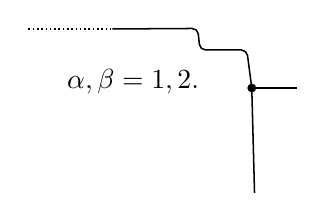
\begin{tikzpicture}[x=.007cm,y=-.007cm,line width=.55pt,every node/.style={inner sep=0pt}]
\draw[densely dotted] (15,32)--(167,32);
\draw[rounded corners=2pt] (167,32)--(322,31)--(326,70)--(411,70)--(420,139);
\draw (420,139)--(425,329);
\draw (420,139)--(502,139);
\fill (420,139) circle[radius=1.6pt];
\node[anchor=west] at (84,128) {\(\alpha,\beta=1,2.\)};
\end{tikzpicture}}\endgroup\par
Ступенчатая линия между формулой для индексов и правой заметкой. От точки вправо отходит короткая черта. Привязка черт к строкам неясна.}
\end{GelfandAdjacentEvidence}
\begin{GelfandAdjacentEvidence}{GELFAND-P000849}{10}


[Основной текст:] Если гр. Лоренца или \(SO(4)\)
\[
\Omega_\alpha^\beta=(\omega^{ab}\Sigma_{ab})_\alpha^\beta \tag{2}
\]
\(\alpha,\beta=1,2.\)

(закон преобр. 2-х комп. спинора)

\(\Sigma_{ab}\) — фиксир. матрицы (вроде матр. Паули) 2-го порядка

\(\omega^{ab}\) — параметры

Для матриц Паули
\[
\sigma_i\sigma_j=\delta_{ij}+\epsilon_{ijk}\sigma^k \tag{3}
\]
\Unclear{GELFAND-P000849}{pauli-product-source}{После знака плюс в (3) видна буква \(\epsilon\). Перед ней нет отдельного множителя.}
\end{GelfandAdjacentEvidence}
\begin{GelfandAdjacentEvidence}{GELFAND-P000849}{11}

\[
\sigma^a=(I,i\vec\sigma),\qquad a=1,2,3,4.
\]
\[
\Sigma_{ab}=\sigma_a\bar\sigma_b-\bar\sigma_b\sigma_a \tag{4}
\]

Теперь о величинах в спинорных обозначениях.

\uwave{Пенроуз} сформулировал так теорию гравитации.

Пусть есть вектор \(x_a\); тогда
\[
X_{\alpha\dot\alpha}=\sigma^a_{\alpha\dot\alpha}x_a\quad\text{— спинор} \tag{5}
\]
\[
\Psi_{\alpha_1\ldots\alpha_{2A},\dot\alpha_1\ldots\dot\alpha_{2B}}=\Psi(A,B) \tag{6}
\]
\Unclear{GELFAND-P000849}{equation-six-first-dotted-index}{Первый индекс с точкой предварительно набран \(\dot\alpha_1\). Начертание цифры можно прочесть и как 2.}
\end{GelfandAdjacentEvidence}



\Needspace{7\baselineskip}
\begin{GelfandAdjacentEvidence}{GELFAND-P000850}{1}
\SourcePage{GELFAND-P000850}{2}
и если произвести полную симметризацию, то получится неприв. представление.

Кстати о матрицах Паули: они таковы.
\[
\left\{\begin{aligned}
\sigma^1_{\alpha\dot\alpha}&=\frac{1}{\sqrt2}\begin{pmatrix}0&1\\1&0\end{pmatrix};\\
\sigma^2_{\alpha\dot\alpha}&=\frac{1}{\sqrt2}\begin{pmatrix}0&-i\\i&0\end{pmatrix};\\
\sigma^3_{\alpha\dot\alpha}&=\frac{1}{\sqrt2}\begin{pmatrix}1&0\\0&-1\end{pmatrix};\\
\sigma^4_{\alpha\dot\alpha}&=\frac{1}{\sqrt2}\begin{pmatrix}1&0\\0&1\end{pmatrix}.
\end{aligned}\right. \tag{7}
\]
\Unclear{GELFAND-P000850}{pauli-first-index-overwritten}{Первый нижний индекс в \(\sigma^1\) переписан. Сверху читается \(\alpha\), прежний знак не читается.}
\end{GelfandAdjacentEvidence}
\begin{GelfandAdjacentEvidence}{GELFAND-P000850}{2}


Есть ещё \(\epsilon^{\alpha\beta}\)
\[
\epsilon^{12}=1,\qquad\epsilon_{\alpha\beta}=\begin{bmatrix}0&1\\-1&0\end{bmatrix} \tag{8}
\]

Опускание индексов:
\[
\Psi_\alpha=\epsilon_{\alpha\beta}\Psi^\beta \tag{9}
\]

\uline{И. М. Г.}

По коорд. \(\dot\alpha\) преобраз. комплексно сопряженное.

Ф-ла (5) — \uwave{констр. спинора по вектору}
\SourceFigure{GELFAND-P000850}{circled-emphasis}{%
\begingroup\color{black}\GelfandFitDiagram{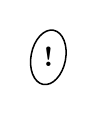
\begin{tikzpicture}[line width=.55pt]
\draw[rotate=-11] (0,0) ellipse[x radius=.22cm,y radius=.35cm];
\node[font=\bfseries] at (0,0) {!};
\end{tikzpicture}}\endgroup\par
Обведённый восклицательный знак слева от строки о формуле (5).}
\end{GelfandAdjacentEvidence}
\begin{GelfandAdjacentEvidence}{GELFAND-P000850}{3}

\SourceFigure{GELFAND-P000850}{spinor-divider}{%
\begingroup\color{black}\GelfandFitDiagram{\begin{tikzpicture}[x=.01cm,y=-.01cm,line width=.55pt]
\draw (19,29)--(72,29);
\fill (98,29) circle[radius=1.4pt];
\draw (145,23)--(241,23);
\end{tikzpicture}}\endgroup}
\end{GelfandAdjacentEvidence}
\begin{GelfandAdjacentEvidence}{GELFAND-P000850}{4}


\uline{К.} Рассм. [зачёркнуто: \sout{…}] теперь антисимметр. тензоры
\Incomplete{GELFAND-P000850}{before-antisymmetric-cancelled}{Перед «теперь» слово зачёркнуто. Оно не читается.}
\end{GelfandAdjacentEvidence}
\begin{GelfandAdjacentEvidence}{GELFAND-P000850}{5}

\[
\begin{aligned}
F_{[ab]}\longmapsto F_{\alpha\beta\dot\gamma\dot\delta}
&=\epsilon_{\alpha\gamma}F_{\dot\beta\dot\delta}
+\epsilon_{\dot\beta\dot\delta}F_{\alpha\gamma},
\end{aligned} \tag{10}
\]
\Unclear{GELFAND-P000850}{tensor-index-order}{У тензора слева от равенства точки видны над третьим и четвёртым индексами. Справа точки стоят над индексами, предварительно прочитанными как \(\beta,\delta\).}
\end{GelfandAdjacentEvidence}
\begin{GelfandAdjacentEvidence}{GELFAND-P000850}{6}


[Под \(F_{[ab]}\):] антисимм. тензор

(это только для антисимм.)

— легко проверить

[Справа:] \(F_{\alpha\gamma},F_{\dot\beta\dot\delta}\) — симм. тензоры

[На правом поле:]
\[
\begin{aligned}
\Lambda^2(S\otimes\bar S)&=\Lambda^2S\otimes S^2\bar S+S^2(S)\\
 &\qquad\qquad\otimes\Lambda^2\bar S
\end{aligned} \tag{*}
\]
\Unclear{GELFAND-P000850}{star-right-edge}{Второе слагаемое перенесено. После \(S^2\) буква \(S\), по-видимому, взята в скобки.}
\end{GelfandAdjacentEvidence}
\begin{GelfandAdjacentEvidence}{GELFAND-P000850}{7}

соб. знач. опер. \(*\) — \(\pm1\)

\uwave{Самодуальный тензор}: опр. опер. \(*\):
\[
{}^*F_{ab}=\frac12\epsilon_{abcd}F^{cd} \tag{11}
\]

\uwave{самодуальность}:
\[
F_{ab}=\pm{}^*F_{ab};\quad
\text{[зачёркнуто: …]}\quad
\{F_{\alpha\beta}=0\quad\text{или}\quad F_{\dot\alpha\dot\beta}=0\} \tag{12}
\]
\Incomplete{GELFAND-P000850}{selfduality-cancelled}{Зачёркнутая запись перед фигурной скобкой не читается.}
\end{GelfandAdjacentEvidence}
\begin{GelfandAdjacentEvidence}{GELFAND-P000850}{8}


\uline{О гравитации}

\uwave{Тензор кривизны}: \(R_{abcd}\). Считается, что есть метрика

и определение операции \(*\):
\[
{}^*R_{abcd}=\frac12\epsilon_{ab}{}^{c'd'}R_{c'd'cd} \tag{13}
\]
\Incomplete{GELFAND-P000850}{curvature-faint-trailing}{Справа от (13) видны бледные штрихи. Запись по ним не восстанавливается.}
\end{GelfandAdjacentEvidence}
\begin{GelfandAdjacentEvidence}{GELFAND-P000850}{9}


Спинорный эквивалент. Ур-я Эйнш. вытек. из усл. самодуальности

(и найдено много гравит. инстантонов)
\Unclear{GELFAND-P000850}{einstein-parenthesis}{Слово после «и» предварительно прочитано «найдено».}
\end{GelfandAdjacentEvidence}
\begin{GelfandAdjacentEvidence}{GELFAND-P000850}{10}

\[
R_{\alpha\beta\gamma\delta}\quad\text{и}\quad R_{\dot\alpha\dot\beta\dot\gamma\dot\delta}
\]
\[
R_+=R+{}^*R=0\quad\text{— см. ур-е}\ (*).
\]

[Справа:] см. лекц. Хокинга, 1978 г. со ссылкой на Пенроуза
\SourceFigure{GELFAND-P000850}{penrose-reference-bracket}{%
\begingroup\color{black}\GelfandFitDiagram{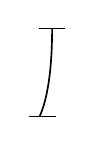
\begin{tikzpicture}[x=.01cm,y=-.01cm,line width=.6pt]
\draw (29,18)--(62,18);
\draw (46,18) .. controls (46,66) and (41,106) .. (30,130);
\draw (16,130)--(51,130);
\end{tikzpicture}}\endgroup\par
Вертикальная помета с поперечными чертами слева от ссылки на лекции.}
\end{GelfandAdjacentEvidence}
\begin{GelfandAdjacentEvidence}{GELFAND-P000850}{11}


\[
\Phi(A,B)=\Psi_{\alpha_1,\ldots,\alpha_{2A},\dot\alpha_1,\ldots,\dot\alpha_{2B}} \tag{14}
\]
\Unclear{GELFAND-P000850}{phi-overwrite}{Буква в (14) набрана как \(\Phi\). Неясно, является ли верхний штрих отдельной чертой.}
\end{GelfandAdjacentEvidence}
\begin{GelfandAdjacentEvidence}{GELFAND-P000850}{12}


Ур-я сод. кучу разных ур-й — Максвелл, де Вит, Швингер, Эйнштейн, Ходж — де Рам (для дифф. форм).
\Unclear{GELFAND-P000850}{final-list}{В списке фамилий имя после «де Вит» предварительно прочитано «Швингер».}
\end{GelfandAdjacentEvidence}


(см. [3])


\Needspace{7\baselineskip}
\begin{GelfandAdjacentEvidence}{GELFAND-P000851}{1}
\SourcePage{GELFAND-P000851}{unlabelled}
Спинор пока симметр. (соотв. неприв. предст.). Определение \(\Delta\).
\Unclear{GELFAND-P000851}{spinor-opening}{Сокращение перед «неприв.» предварительно прочитано «соотв.».}
\end{GelfandAdjacentEvidence}
\begin{GelfandAdjacentEvidence}{GELFAND-P000851}{2}

\[
\begin{aligned}
(\Delta\phi)_{\alpha_1\ldots\alpha_{2A},\dot\alpha_1\ldots\dot\alpha_{2B}}
&=\bigl(-\Box\epsilon_{\alpha_1\beta}
+2\nabla_{\dot\xi(\alpha_1}\nabla^{\dot\xi}_{\beta)}\bigr)\\[-.15em]
&\qquad{}\bar\phi^{\beta}{}_{\alpha_2\ldots\alpha_{2A},\dot\alpha_1\ldots\dot\alpha_{2B}}.
\end{aligned}\tag{15}
\]
\Unclear{GELFAND-P000851}{delta-operator-indices}{Маленькие точки в свёртке предварительно отнесены к двум индексам \(\xi\). Нижние \(\alpha_1,\beta\) охвачены скобками.}
\end{GelfandAdjacentEvidence}
\begin{GelfandAdjacentEvidence}{GELFAND-P000851}{3}

\Unclear{GELFAND-P000851}{delta-barred-field}{На правой стороне (15) предварительно набрано \(\bar\phi^\beta\). Над буквой видна короткая черта.}
\end{GelfandAdjacentEvidence}
\begin{GelfandAdjacentEvidence}{GELFAND-P000851}{4}


\uline{Свойства}.
\[
1)\qquad(\phi,\Delta\phi)=(\Delta\phi,\phi)\tag{16}
\]
\[
2)\qquad \Delta\phi(0,0)=-\Box\phi,\qquad
\text{здесь}\quad\Box=\nabla_{\alpha\dot\alpha}\nabla^{\alpha\dot\alpha},\tag{17}
\]
\[
\nabla_{\alpha\dot\alpha}=\sigma^a_{\alpha\dot\alpha}\mathcal{D}_a;
\qquad \mathcal{D}_a=\partial_a+B_a
\]

3) Dirac \(\phi(1/2,0)\) (в кривом пр-ве)
\[
\Psi_\pm=(1\pm\gamma_5)\Psi,\tag{18}
\]
\Unclear{GELFAND-P000851}{dirac-projection}{После 5 виден короткий горизонтальный штрих. Его назначение неясно.}
\end{GelfandAdjacentEvidence}
\begin{GelfandAdjacentEvidence}{GELFAND-P000851}{5}

\(\Psi\) — 4-компон. Дираковский спинор
\[
\Delta\Psi_\pm=\left(-\Box+\frac14R\right)\Psi_\pm
\]
\SourceFigure{GELFAND-P000851}{scalar-curvature-marker}{%
\begingroup\color{black}\GelfandFitDiagram{\begin{tikzpicture}[every node/.style={inner sep=1pt},line width=.55pt]
\node (r) at (0,0) {\(R\)};
\draw (0,-.18)--(-.09,-.48);
\node[align=left,anchor=north] at (-.10,-.56) {скал.\\кривизна};
\end{tikzpicture}}\endgroup\par
Штрих под \(R\) ведёт к подписи.}
\end{GelfandAdjacentEvidence}
\begin{GelfandAdjacentEvidence}{GELFAND-P000851}{6}


4) Максвелл в гарм. калибровке
\Unclear{GELFAND-P000851}{maxwell-gauge-abbreviation}{Сокращение перед «калибровке» предварительно прочитано «гарм.».}
\end{GelfandAdjacentEvidence}
\begin{GelfandAdjacentEvidence}{GELFAND-P000851}{7}

\[
\Delta A_a=(-\Box g_{ab}+R_{ab})A^b,\qquad
\mathcal{D}^aA_a=0\tag{19}
\]
\Unclear{GELFAND-P000851}{maxwell-overwritten-operator}{Оператор перед \(A_a\) сильно переправлен. Предварительно набрано \(\mathcal{D}\). Возможно \(\nabla\).}
\end{GelfandAdjacentEvidence}
\begin{GelfandAdjacentEvidence}{GELFAND-P000851}{8}

\[
5)\qquad\underline{s=\frac32}\qquad\text{кого то и Швингера}\tag{20}
\]
\Unclear{GELFAND-P000851}{schwinger-line}{Первые слова предварительно прочитаны «кого то». Имя перед «и Швингера» не выписано.}
\end{GelfandAdjacentEvidence}
\begin{GelfandAdjacentEvidence}{GELFAND-P000851}{9}

\[
6)\quad\underline{s=2}\quad\text{Эйнштейн}\tag{21}
\]
\[
7)\qquad w=\frac1{p!}\omega_{\mu_1\ldots\mu_p}\,dx^{\mu_1}\wedge\ldots\wedge dx^{\mu_p}\tag{22}
\]
\Unclear{GELFAND-P000851}{differential-forms-first-symbol}{Слева от равенства знак похож на латинское \(w\). Справа при индексах — \(\omega\).}
\end{GelfandAdjacentEvidence}
\begin{GelfandAdjacentEvidence}{GELFAND-P000851}{10}

\[
\phi(0,0),\quad\phi(1/2,1/2),\quad\phi(1,0),\quad\phi(0,1)
\]
\[
\Delta=\delta d+d\delta
\]

[зачёркнуто: \sout{…}] Станд. теория дифф. форм опис. \uuline{бозоны}.
\Incomplete{GELFAND-P000851}{before-standard-cancelled}{Перед «Станд.» зачёркнут знак. Исходное начертание не читается.}
\end{GelfandAdjacentEvidence}
\begin{GelfandAdjacentEvidence}{GELFAND-P000851}{11}


Если бы были нечётные — то вся мат.
\Unclear{GELFAND-P000851}{whole-mat}{Строка оканчивается сокращением «мат.» без продолжения.}
\end{GelfandAdjacentEvidence}
\begin{GelfandAdjacentEvidence}{GELFAND-P000851}{12}


[3] — на форму навесили чётные инд.
\Unclear{GELFAND-P000851}{before-indices}{Последнее прилагательное предварительно прочитано «чётные». Его начальные штрихи бледные.}
\end{GelfandAdjacentEvidence}
\begin{GelfandAdjacentEvidence}{GELFAND-P000851}{13}


\uwave{Надо}: сделать антикоммутирующие \(dx\).

[Справа:] Березин частично сделал.

Пока нет [зачёркнуто: \sout{… …}]
\Incomplete{GELFAND-P000851}{after-poka-cancelled}{Два зачёркнутых слова после «нет» не читаются.}
\end{GelfandAdjacentEvidence}

дифф. форм, сод. среди \(dx\) \uwave{комм. и антикоммут.}

ввести оператор \(\Delta\) и построить \uwave{теор. индекса}

Бозонное поле \(\Psi_a\) даёт форму \(\Psi_a dx^a\).

Для спина \(\frac52\) все ур-я не годятся (не удаётся сделать взаимодействие)

— „ — \(\frac32\) только что сделано (супергравитация)

\uwave{Идея И. М. Г.} возможно, не обязательно \(d\delta+\delta d\).


\Needspace{7\baselineskip}
\begin{GelfandAdjacentEvidence}{GELFAND-P000852}{1}
\SourcePage{GELFAND-P000852}{3}
Эквивалентная форма записи \(\Delta\):
\[
\Delta=-\Box+X,\tag{23}
\]
\[
X=-\Sigma^{ab}R_{ab}^{cd}\Sigma_{cd},\qquad A+B\text{ — целое}\tag{24}
\]
\[
X=-\frac{1}{A}\Sigma^{ab}R_{+ab}^{cd}\Sigma_{cd},\qquad
A+B\text{ — полуцелое},\quad A>B.\tag{25}
\]
\Unclear{GELFAND-P000852}{half-integer-abbreviation}{Буква \(B\) в условии \(A+B\) сильно обведена. Начертание под обводкой не различается.}
\end{GelfandAdjacentEvidence}
\begin{GelfandAdjacentEvidence}{GELFAND-P000852}{2}

\SourceFigure{GELFAND-P000852}{curvature-insertion}{%
\begingroup\color{black}\GelfandFitDiagram{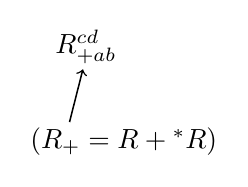
\begin{tikzpicture}[line width=.55pt,every node/.style={inner sep=1pt}]
\node at (0,1.2) {\(R_{+ab}^{cd}\)};
\node at (.48,0) {\((R_+=R+{}^*R)\)};
\draw[->] (-.21,.25)--(-.04,.92);
\end{tikzpicture}}\endgroup\par
Стрелка ведёт от вставки к переправленному нижнему знаку при \(R\) в (25).}
\end{GelfandAdjacentEvidence}
\begin{GelfandAdjacentEvidence}{GELFAND-P000852}{3}


\(\varphi\) здесь симметрична по \(\alpha_1\ldots\alpha_{2A}\) и по \(\dot\alpha_1\ldots\dot\alpha_{2B}\).
\[
\Delta\varphi=\lambda\varphi\tag{26}
\]
\Unclear{GELFAND-P000852}{eigenfield-overwrite}{Знак после \(\Delta\) в (26) переправлен. Предварительно набрано \(\varphi\).}
\end{GelfandAdjacentEvidence}
\begin{GelfandAdjacentEvidence}{GELFAND-P000852}{4}


Отсюда будет следовать условие совместности.
\SourceFigure{GELFAND-P000852}{circled-symmetry-insertion}{%
\begingroup\color{black}\GelfandFitDiagram{\begin{tikzpicture}[line width=.55pt,every node/.style={inner sep=2pt}]
\node (old) at (0,-.04) {\sout{(26)}};
\node[draw,rounded corners=5pt] (sym) at (2.55,.06) {(и из симметрии)};
\draw[->] (old.east)--(sym.west);
\end{tikzpicture}}\endgroup\par
Черта через зачёркнутый номер (26) переходит в стрелку к обведённой вставке.}
\end{GelfandAdjacentEvidence}
\begin{GelfandAdjacentEvidence}{GELFAND-P000852}{5}


\uwave{Условие совместности}:
\[
\nabla_{\dot\alpha}^{(\alpha_1}\nabla^{\alpha_2)\dot\alpha}
\varphi_{\alpha_1\alpha_2\ldots\alpha_{2A},\dot\alpha_1\ldots\dot\alpha_{2B}}=0
\tag{27}
\]
\Unclear{GELFAND-P000852}{equation27-number}{Последняя цифра переправлена. Предварительно набрано (27). Возможно (28).}
\end{GelfandAdjacentEvidence}
\begin{GelfandAdjacentEvidence}{GELFAND-P000852}{6}

\(A\leq1\), \(B\leq1\) \(\Rightarrow\) случай всех физ. полей

Рассм. ур-е теплопроводности
\[
\frac{d}{dt}F(x,x',t)+\Delta F(x,x',t)=0,\qquad
F\big|_{t=0}=\delta(x-x').\tag{28}
\]
на компактном мн-зии
\[
\operatorname{Tr}F(x,x,t)\underset{t\to+0}{\sim}
\sum_{k=0}^{\infty}b_k\,t^{(k-4)/2}\tag{29}
\]
\Unclear{GELFAND-P000852}{equation29-coefficient-edit}{Перед \(t\) виден переправленный знак, возможно зачёркнутое \((x)\).}
\end{GelfandAdjacentEvidence}
\begin{GelfandAdjacentEvidence}{GELFAND-P000852}{7}

\Incomplete{GELFAND-P000852}{equation29-exponent-deletion}{Перед показателем \((k-4)/2\) прежняя запись зачёркнута и не читается.}
\end{GelfandAdjacentEvidence}
\begin{GelfandAdjacentEvidence}{GELFAND-P000852}{8}

\[
B_k=\int d^4x\sqrt{g}\,b_k,\tag{30}
\]
Тогда
\[
B_4=n+m.\tag{31}
\]
[Справа:] \(B_4\) — первый нерасходящийся.

\(n\) — число 0-х соб. значений (26)

\(m\) — [зачёркнуто: \sout{число ненулевых соб. знач.}]
[Вписано ниже:] кратность ненулевого (любого) соб. знач.

[Справа:] [их общая кратность — все кратности одинаковы!!]
\SourceFigure{GELFAND-P000852}{multiplicity-correction}{%
\begingroup\color{black}\GelfandFitDiagram{\begin{tikzpicture}[line width=.55pt,every node/.style={inner sep=1pt}]
\node[anchor=west] at (0,1.25) {— гипотеза С. Гельфанда};
\node[anchor=west] at (.48,0) {\uwave{неверно.}};
\draw[->] (.53,.29)--(.55,.92);
\end{tikzpicture}}\endgroup\par
Стрелка от подчёркнутого «неверно» идёт вверх к записи о гипотезе.}
\end{GelfandAdjacentEvidence}
\begin{GelfandAdjacentEvidence}{GELFAND-P000852}{9}


Цель — выраз. через топ. инварианты.

\uwave{Gilkey} дошел до \(\underline{\underline{B_6}}\). (1975)
\Unclear{GELFAND-P000852}{gilkey-coefficient}{Переправленная буква предварительно набрана \(B\). Возможно \(b\).}
\end{GelfandAdjacentEvidence}
\begin{GelfandAdjacentEvidence}{GELFAND-P000852}{10}


\SourceFigure{GELFAND-P000852}{gilkey-leaders}{%
\begingroup\color{black}\GelfandFitDiagram{\begin{tikzpicture}[line width=.55pt,every node/.style={inner sep=1pt}]
\node (b) at (0,1.1) {\(\underline{\underline{B_6}}\)};
\node (d) at (3.10,1.1) {(1975)};
\node (y) at (.19,-.2) {1979 есть (И. М. Г.)};
\node (r) at (3.13,.25) {ссылка здесь такая};
\draw (b.south)--(y.north);
\draw (d.south)--(r.north);
\end{tikzpicture}}\endgroup\par
Две короткие черты связывают верхние знаки с приписками под ними.}
\end{GelfandAdjacentEvidence}
\begin{GelfandAdjacentEvidence}{GELFAND-P000852}{11}

\Unclear{GELFAND-P000852}{gilkey-year-word}{После 1979 предварительно прочитано «есть». Возможно «ещё».}
\end{GelfandAdjacentEvidence}
\begin{GelfandAdjacentEvidence}{GELFAND-P000852}{12}

\Unclear{GELFAND-P000852}{gilkey-reference-word}{Последнее слово после «ссылка здесь» предварительно прочитано «такая».}
\end{GelfandAdjacentEvidence}
\begin{GelfandAdjacentEvidence}{GELFAND-P000852}{13}


Если есть граница, то тоже \(b_4\) сейчас [зачёркнуто: \sout{…}] недавно написано; вопрос счит. сложным.
\Unclear{GELFAND-P000852}{boundary-coefficient}{Коэффициент в строке о границе предварительно прочитан \(b_4\).}
\end{GelfandAdjacentEvidence}
\begin{GelfandAdjacentEvidence}{GELFAND-P000852}{14}

\Incomplete{GELFAND-P000852}{boundary-deleted-word}{Слово перед «недавно» зачёркнуто и не читается.}
\end{GelfandAdjacentEvidence}
\begin{GelfandAdjacentEvidence}{GELFAND-P000852}{15}


Рассм. приводимые предст.
\[
\varphi_{\alpha\beta}=\varphi_{(\alpha\beta)}
+\frac12\varepsilon_{\alpha\beta}\varphi_{\alpha}^{\alpha}\tag{32}
\]
\[
[1,0]=(1,0)\oplus(0,0)
\]
В силу условий совместности
\[
[\nabla_{\alpha}^{\dot\alpha},\Delta]\varphi[A,B]=0\tag{33}
\]
\Unclear{GELFAND-P000852}{compatibility-commutator}{Над верхней \(\alpha\) виден маленький штрих. Предварительно принят за точку.}
\end{GelfandAdjacentEvidence}



\Needspace{7\baselineskip}
\begin{GelfandAdjacentEvidence}{GELFAND-P000853}{1}
\SourcePage{GELFAND-P000853}{unlabelled}
\[
(\Delta-\lambda)\varphi_{\alpha_1\ldots}=0\tag{34}
\]
Рассм.
\[
\begin{aligned}
\Psi_{\alpha_1\ldots\alpha_{2A-1}\dot\alpha_1\ldots\dot\alpha_{2B+1}}
={}&\nabla_{\dot\alpha_{2B+1}}^{\alpha_{2A}}\\[-.15em]
&\qquad\varphi_{\alpha_1\ldots\alpha_{2A}\dot\alpha_1\ldots\dot\alpha_{2B}}
\end{aligned}\tag{35}
\]
\Unclear{GELFAND-P000853}{equation35-dot-order}{В (35) точка относится к нижнему индексу производной. Верхний предварительно прочитан как \(\alpha_{2A}\).}
\end{GelfandAdjacentEvidence}
\begin{GelfandAdjacentEvidence}{GELFAND-P000853}{2}


\(\Psi\ne0\) при \(\varphi\ne0\) (иначе \(\overset{\circ}{\times}\) с (34)).
\Unclear{GELFAND-P000853}{after35-symbol}{Маленький овал над косым крестом предварительно набран как кружок. Значение записи неясно.}
\end{GelfandAdjacentEvidence}
\begin{GelfandAdjacentEvidence}{GELFAND-P000853}{3}

\[
m[A,B]=m[A-\tfrac12,B+\tfrac12]\tag{36}
\]
\SourceFigure{GELFAND-P000853}{nonzero-modes-leader}{%
\begingroup\color{black}\GelfandFitDiagram{\begin{tikzpicture}[line width=.55pt,every node/.style={inner sep=1pt}]
\node[anchor=west] at (-.05,.85) {\(m[A,B]\)};
\draw (.21,.51)--(.20,.30);
\node[anchor=west] at (0,0) {число ненулев. мод};
\end{tikzpicture}}\endgroup\par
Короткая черта под \(m\) указывает на подпись.}
\end{GelfandAdjacentEvidence}
\begin{GelfandAdjacentEvidence}{GELFAND-P000853}{4}

\[
A+B=S,\qquad A-B=T.
\]
Тогда получаем
\[
m[S,T]=m[S]\tag{37}
\]
Отсюда
\[
n[S,T]-n[S,T']=B_4[S,T]-B_4[S,T']\tag{38}
\]
\[
n[S,T]-n[S,T-1]=4^{s-1}\bigl((T-\tfrac12)\chi+(s-\tfrac23)\tfrac{p}{2}\bigr)\tag{39}
\]
\Unclear{GELFAND-P000853}{index39-lettercase}{Буквы справа в (39) предварительно прочитаны как строчные \(s\). Слева обозначение выглядит как прописная \(S\).}
\end{GelfandAdjacentEvidence}
\begin{GelfandAdjacentEvidence}{GELFAND-P000853}{5}


\(\chi\) — число Эйлера, \(p\) — число Понтрягина

\uwave{Об ур-и теплопров}.
\Unclear{GELFAND-P000853}{heat-heading}{Конец подчёркнутого заголовка предварительно прочитан «теплопров.».}
\end{GelfandAdjacentEvidence}
\begin{GelfandAdjacentEvidence}{GELFAND-P000853}{6}

\[
F(x,x',t)=\sum_{i=0}^{\infty}\varphi_i(x)\varphi_i(x')e^{-\lambda_i t}\tag{40}
\]
\(\varphi_i\) — ортонорм. сист.
\[
F(x,x',0)=\delta(x,x')\tag{41}
\]
\[
\int_M d^4x\sqrt{g}\,F(x,x,t)
=\sum_{i=0}^{\infty}e^{-\lambda_i t}
=n+\sum_{i=n+1}^{\infty}e^{-\lambda_i t}\tag{42}
\]
\Unclear{GELFAND-P000853}{equation42-deleted-mark}{Над вторым \(x\) зачернён маленький знак, возможно штрих.}
\end{GelfandAdjacentEvidence}
\begin{GelfandAdjacentEvidence}{GELFAND-P000853}{7}

\[
F(x,x,t)\sim\sum_{k=0}^{\infty}b_k(x)t^{(k-4/2}\tag{43}
\]
\Unclear{GELFAND-P000853}{equation43-exponent}{Цифра 4 переправлена. Самостоятельная закрывающая скобка перед дробной чертой не различима.}
\end{GelfandAdjacentEvidence}
\begin{GelfandAdjacentEvidence}{GELFAND-P000853}{8}


\(m\) опред. отсюда!! — выкидыванием расх. членов \(\sum e^{-\lambda_i t}\) и \(n\) \uline{даёт вклад}.

\uwave{\(m\) — регуляриз. сумма}
\Unclear{GELFAND-P000853}{regularized-sum}{Сокращение в подчёркнутой помете предварительно прочитано «регуляриз.».}
\end{GelfandAdjacentEvidence}
\begin{GelfandAdjacentEvidence}{GELFAND-P000853}{9}


«\(m\) — целое (!) из глубоких топ. соображений »

Это станд. однопетлевые расх. контин. интеграла.
\Unclear{GELFAND-P000853}{integral-abbreviation}{Конец строки предварительно прочитан «контин. интеграла». Последнее слово выглядит как форма родительного падежа.}
\end{GelfandAdjacentEvidence}
\begin{GelfandAdjacentEvidence}{GELFAND-P000853}{10}


[Справа: в?]
\Unclear{GELFAND-P000853}{isolated-mark}{Отдельный тёмный знак может быть буквой «в». Его чтение не установлено.}
\end{GelfandAdjacentEvidence}
\begin{GelfandAdjacentEvidence}{GELFAND-P000853}{11}


Опред. \(\chi\) и \(p\) для мн-зий без края
\[
\chi=\int {}^*R_{abcd}\,{}^*R^{abcd}\,d^4x\sqrt{g}\tag{44}
\]
\Unclear{GELFAND-P000853}{curvature-stars}{В (44) перед обоими \(R\) различимы звёздочки.}
\end{GelfandAdjacentEvidence}

\[
p=\int {}^*R_{abcd}R^{abcd}\,d^4x\,\sqrt{g}\tag{45}
\]


\Needspace{7\baselineskip}
\begin{GelfandAdjacentEvidence}{GELFAND-P000854}{1}
\SourcePage{GELFAND-P000854}{4}
\uline{8.10.79.} \quad \uline{Сем. Гельфанда.}

\uline{Проект теор. минимума}, \uline{необх. при любой специализации}. (для 1-курсников)

1. \uline{Алгебра}

Ван дер Варден, гл. 1–5, 12.

Гельфанд лекции по лин. алгебре

Атья, Макдональд

2. \uline{Анализ}
\SourceFigure{GELFAND-P000854}{analysis-reading-braces}{%
\(\underline{\text{или}}\quad
\left\{\begin{array}{l}
\text{Берс}\\
\text{[зачёркнуто: \sout{…}] Лузин}\\
\text{Берман}
\end{array}\right\}\)
\par\noindent для втузов.
\par\smallskip
потом.
\par\noindent
\(\text{или}\quad
\left\{\begin{array}{l}
\text{Рудин}\\
\text{Дьедонне}\\
\text{Грауэрт, Либ, Фишер}\\
\text{Шварц}
\end{array}\right\}\)
\par\noindent
[Справа:]\par
Спивак\par
Бишоп — Криттенден\par
Номидзу
\par Две пары фигурных скобок объединяют списки. Справа от второй пары три отдельные строки.}
\end{GelfandAdjacentEvidence}
\begin{GelfandAdjacentEvidence}{GELFAND-P000854}{2}

\Unclear{GELFAND-P000854}{analysis-cancelled-name}{Перед «Лузин» зачёркнута фамилия. «Берман» — возможное чтение.}
\end{GelfandAdjacentEvidence}
\begin{GelfandAdjacentEvidence}{GELFAND-P000854}{3}


\uline{Контр. вопрос:} вычислить приблизительно
\[
\begin{aligned}
&\int_{-\infty}^{\infty} e^{-x^2}\cos 1000x\,dx,\qquad
 \int_{-\infty}^{\infty} e^{-1000x^2}\cos x\,dx\\
&\qquad\text{(и сравн. с табл.)}\\[.3em]
&\int_{-\infty}^{\infty} e^{-1000x^4}\cos x\,dx,\qquad
 \int_{-\infty}^{\infty} e^{-x^4}\cos 1000x\,dx
\end{aligned}
\]

3. \uline{Арнольд} \(\mathrm{I},\ \mathrm{II},\ \mathrm{III}.\)

4. \uline{Кириллов} \(\tfrac12+\tfrac12\)

\uline{Серр} лин. предст. конечных групп

(3-ю главу он не понимает)

\uline{Обобщ. ф-и} \(\mathrm{I}\) вып., гл. 1–2

5. \uline{Знать ур-я в частных производных}. (читать нечего).

\uwave{Контр. зад. по лин. алгебре:}

\uwave{найти кан. форму самосопр. опер. в [зачёркнуто: \sout{…}] симплект. пр-ве}.
\Incomplete{GELFAND-P000854}{symplectic-deleted-word}{После «в» слово зачёркнуто и не читается.}
\end{GelfandAdjacentEvidence}
\begin{GelfandAdjacentEvidence}{GELFAND-P000854}{4}

\Unclear{GELFAND-P000854}{symplectic-final-abbreviation}{Сокращение после зачёркнутого слова предварительно прочитано «симплект.».}
\end{GelfandAdjacentEvidence}
\begin{GelfandAdjacentEvidence}{GELFAND-P000854}{5}


6. [зачернено] \uline{Спец. теория отн. \(+\) ОТО}
\Unclear{GELFAND-P000854}{reading6-blackened-mark}{Перед «Спец.» зачернён одиночный знак, возможно буква «А».}
\end{GelfandAdjacentEvidence}
\begin{GelfandAdjacentEvidence}{GELFAND-P000854}{6}


\(+\) \uline{геометрия}

[Справа:] Ландау, Лифшиц ( т. 2)

совм. с Номидзу
\Unclear{GELFAND-P000854}{nomizu-note-abbreviation}{Сокращение перед «с Номидзу» предварительно прочитано «совм.».}
\end{GelfandAdjacentEvidence}
\begin{GelfandAdjacentEvidence}{GELFAND-P000854}{7}


\medskip
\uuline{С. Гиндикин}. \uline{Начала теории твисторов}.

Будет рассказ. на языке интегр. геометрии.

[Справа:] Твисторы ввёл \uline{Пенроуз}.

см. один из посл. номеров BAMS,

1979, т. 1 (нов. серия),

ст. \uline{Уэллса} (\uline{Wells.})

[зачёркнуто: \sout{… рассмотрим?}]
\Incomplete{GELFAND-P000854}{cancelled-before-diagram}{Зачёркнутая строка перед (1) не читается целиком. Последнее слово предварительно прочитано «рассмотрим».}
\end{GelfandAdjacentEvidence}
\begin{GelfandAdjacentEvidence}{GELFAND-P000854}{8}


\SourceFigure{GELFAND-P000854}{twistor-projection}{%
\begingroup\color{black}\GelfandFitDiagram{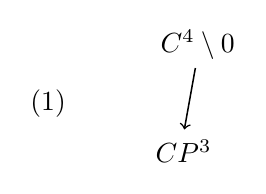
\begin{tikzpicture}[line width=.55pt,every node/.style={inner sep=1pt}]
\node at (-.9,.61) {(1)};
\node (c) at (1,1.35) {\(\mathbb{C}^4\setminus0\)};
\node (p) at (.82,0) {\(\mathbb{C}P^3\)};
\draw[->] (.97,1.06)--(.83,.28);
\end{tikzpicture}}\endgroup}
\end{GelfandAdjacentEvidence}
\begin{GelfandAdjacentEvidence}{GELFAND-P000854}{9}


В \(\mathbb{C}^4\) фиксируем эрмитову форму [зачернено] \((++--)\). \(\langle\ ,\ \rangle\).
\Incomplete{GELFAND-P000854}{hermitian-blackened-symbol}{Перед скобкой со знаками сигнатуры зачернён знак. Он не читается.}
\end{GelfandAdjacentEvidence}


Получаются \(\alpha\)-твисторы: элементы \(\mathbb{C}P^3\) или соотв. элем. \(\mathbb{C}^4\).

\((\mathbb{C}P^3)'\) — двойств. пр-во. Там тоже возник. форма и это — \(\beta\)-твисторы.


\Needspace{7\baselineskip}
\begin{GelfandAdjacentEvidence}{GELFAND-P000855}{1}
\SourcePage{GELFAND-P000855}{unlabelled}
\[
\begin{aligned}
\langle z,z\rangle>0&\Rightarrow\text{полож. твистор}\\
\langle z,z\rangle=0&\Rightarrow\text{нулевой — „ —}\\
\langle z,z\rangle<0&\Rightarrow\text{отриц. — „ —}
\end{aligned}
\]
В \(\mathbb{C}P^3\) рассм. прямые (2-мерн. подпр. в \(\mathbb{C}^4\)).
Их мн-во: \(G=G_{4,2}=G_{4,2}^{\mathbb{C}}\).

Над \(G\) есть натурельное рассл. 2-реперов (главное) в \(\mathbb{C}^4\):
\Unclear{GELFAND-P000855}{bundle-word}{Слово перед «рассл.» предварительно прочитано «натурельное». Середина и конец написаны слитно.}
\end{GelfandAdjacentEvidence}
\begin{GelfandAdjacentEvidence}{GELFAND-P000855}{2}

\SourceFigure{GELFAND-P000855}{bundle-projection}{%
\begingroup\color{black}\GelfandFitDiagram{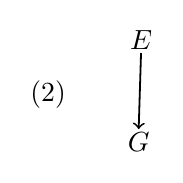
\begin{tikzpicture}[line width=.65pt,every node/.style={inner sep=1pt}]
\node at (-1.18,.61) {(2)};
\node (e) at (0,1.30) {\(E\)};
\node (g) at (-.03,0) {\(G\)};
\draw[->] (e.south)--(g.north);
\end{tikzpicture}}\endgroup}
\end{GelfandAdjacentEvidence}
\begin{GelfandAdjacentEvidence}{GELFAND-P000855}{3}


[Зачёркнуто над заголовком: \sout{В \(\mathbb{C}^4\) …}]
\Incomplete{GELFAND-P000855}{cancelled-heading-line}{В начале зачёркнутой строки, возможно, «В \(\mathbb C^4\)». Полное чтение не установлено.}
\end{GelfandAdjacentEvidence}
\begin{GelfandAdjacentEvidence}{GELFAND-P000855}{4}


[Зачёркнуто слева: \sout{…}] \uwave{Координаты в \(G\)}.
\Incomplete{GELFAND-P000855}{cancelled-heading-prefix}{Слева от заголовка зачёркнута отдельная короткая запись. Она не читается.}
\end{GelfandAdjacentEvidence}
\begin{GelfandAdjacentEvidence}{GELFAND-P000855}{5}


Выберем в \(\mathbb{C}^4\) 2 плоскости (трансверс.) \(L\) и \(L'\), тогда любая другая — график,
матрица соотв. преобр. — координаты.
\SourceFigure{GELFAND-P000855}{inserted-planes}{%
\begingroup\color{black}\GelfandFitDiagram{\begin{tikzpicture}[x=.016cm,y=-.016cm,line width=.55pt,every node/.style={inner sep=1pt}]
\node at (130,41) {\(L\) и \(L'\)};
\draw (47,20) .. controls (48,41) and (87,92) .. (72,112);
\draw (33,141) .. controls (75,118) and (68,104) .. (92,87)
 .. controls (140,49) and (204,92) .. (262,25);
\end{tikzpicture}}\endgroup\par
Знак вставки ведёт к надписанным обозначениям плоскостей.}
\end{GelfandAdjacentEvidence}
\begin{GelfandAdjacentEvidence}{GELFAND-P000855}{6}


Выб. в [зачёркнуто: \sout{…}] \(L\) базис \(e_0\ e_1\); В \(L'\) базис \(e_3,e_4\).
\Incomplete{GELFAND-P000855}{cancelled-before-l}{Запись перед \(L\) зачёркнута и не читается.}
\end{GelfandAdjacentEvidence}
\begin{GelfandAdjacentEvidence}{GELFAND-P000855}{7}

Тогда если \(\widetilde L\in G_{4,2}\), то в \(\widetilde L\) есть базис вида
\Unclear{GELFAND-P000855}{plane-symbol-under-formula}{Повторное обозначение плоскости сильно обведено. Предварительно набрано \(\widetilde L\).}
\end{GelfandAdjacentEvidence}
\begin{GelfandAdjacentEvidence}{GELFAND-P000855}{8}

\[
\begin{cases}
f_0=e_0+u_{03}e_3+u_{04}e_4\\
f_1=e_1+u_{13}e_3+u_{14}e_4
\end{cases}\tag{3}
\]
\Unclear{GELFAND-P000855}{formula-3-index}{Первый подстрочный знак при \(u\) перед \(e_3\) во второй строке предварительно прочитан как 1. Начертание переправлено.}
\end{GelfandAdjacentEvidence}
\begin{GelfandAdjacentEvidence}{GELFAND-P000855}{9}

\(u_{ij}\) — координаты.

Пусть \(L,L'\) трансверс. и изотропные относит. \(\langle\cdot,\cdot\rangle\).
\uline{Задача}. Такие \(L\) и \(L'\) существуют.
\[
\{e_A,\ A=0,1\}\text{ — базис в } L.\tag{4}
\]
В \(L'\) введ. базис
\[
\{e^{A'},\ A'=0',1'\}\text{ — базис в } L'\tag{5}
\]

[зачёркнуто: \sout{…}] [над строкой: Пусть [зачёркнуто: \sout{…}]]
форма [над строкой: \(\langle\ ,\ \rangle\)] в базисе
\((e_0,e_1,e^{0'},e^{1'})\) имеет [зачёркнуто: \sout{…}] матрицу
\Incomplete{GELFAND-P000855}{cancelled-form-prefix}{Перед «форма» на основной строке зачёркнута запись. Она не читается.}
\end{GelfandAdjacentEvidence}
\begin{GelfandAdjacentEvidence}{GELFAND-P000855}{10}

\Incomplete{GELFAND-P000855}{cancelled-after-pust}{После вставленного «Пусть» зачёркнут короткий знак. Он не читается.}
\end{GelfandAdjacentEvidence}
\begin{GelfandAdjacentEvidence}{GELFAND-P000855}{11}

\Incomplete{GELFAND-P000855}{cancelled-before-matrix}{Между «имеет» и «матрицу» слово зачёркнуто. Оно не читается.}
\end{GelfandAdjacentEvidence}
\begin{GelfandAdjacentEvidence}{GELFAND-P000855}{12}

\SourceFigure{GELFAND-P000855}{form-insertions}{%
\begingroup\color{black}\GelfandFitDiagram{\begin{tikzpicture}[line width=.55pt,every node/.style={inner sep=1pt}]
\node at (.38,.83) {Пусть \sout{…}};
\node at (2.56,.83) {\(\langle\ ,\ \rangle\)};
\draw (-.26,.56) .. controls (.14,.48) and (.56,.61) .. (.70,.13)
 .. controls (.75,.45) and (.97,.48) .. (1.25,.58);
\draw (2.15,.61) .. controls (2.23,.49) and (2.47,.37) .. (2.49,.16)
 .. controls (2.62,.54) and (3.00,.46) .. (3.17,.62);
\node at (.07,-.03) {\sout{…}};
\node at (1.55,-.03) {форма};
\node at (3.26,-.03) {в базисе};
\end{tikzpicture}}\endgroup\par
Две пометы обозначают места вставок «Пусть» и угловых скобок.}
\end{GelfandAdjacentEvidence}
\begin{GelfandAdjacentEvidence}{GELFAND-P000855}{13}

\[
\begin{pmatrix}0&iE\\-iE&0\end{pmatrix};\tag{6}
\]
т. е.
\[
\langle e_0,e^{0'}\rangle=\langle e_1,e^{1'}\rangle=i,
\qquad\text{остальные скал. произв. }=0\tag{7}
\]
Сделаем замену переменных в \(L\):
\[
\widetilde e_B=g_B^A e_A\tag{8}
\]
Тогда легко проверить, что
\[
e^{A'}\text{ преобр. с помощью }(g^*)^{-1}\tag{9}
\]
(выводится из соотн. [зачёркнуто: \sout{…}] ортогональности)
\Incomplete{GELFAND-P000855}{cancelled-orthogonality-word}{Перед «ортогональности» зачёркнута запись. Она не читается.}
\end{GelfandAdjacentEvidence}
\begin{GelfandAdjacentEvidence}{GELFAND-P000855}{14}


Есть и другие законы преобр.:
[Зачёркнуто слева: \sout{…}]
\Incomplete{GELFAND-P000855}{cancelled-index-intro}{Перед строками с индексами зачёркнут знак. Он не читается.}
\end{GelfandAdjacentEvidence}
\begin{GelfandAdjacentEvidence}{GELFAND-P000855}{15}

\SourceFigure{GELFAND-P000855}{index-transformation-arcs}{%
\begingroup\color{black}\GelfandFitDiagram{\begin{tikzpicture}[line width=.55pt,every node/.style={inner sep=1pt}]
\node at (.22,1.12) {\(A'\)};
\node[anchor=west] at (.58,1.12) {с пом. \(\bar g\)};
\node at (.22,.05) {\(B\)};
\node[anchor=west] at (.58,.05) {— „ — \((g^T)^{-1}\)};
\node at (3.23,1.12) {\(B'\)};
\node[anchor=west] at (3.60,1.12) {с пом. \((g^*)^{-1}\)};
\draw (-.04,.88) .. controls (-.03,1.07) and (.22,1.66) .. (.40,1.47)
 .. controls (.48,1.39) and (.47,1.19) .. (.44,1.01);
\draw (.04,.20) .. controls (-.01,-.43) and (.32,-.17) .. (.47,.17);
\draw (3.03,1.33) .. controls (2.82,.67) and (3.23,.75) .. (3.55,1.26);
\end{tikzpicture}}\endgroup\par
Дуга огибает \(A'\) сверху, а \(B\) и \(B'\) снизу. Значение дуг не установлено.}
\end{GelfandAdjacentEvidence}



\Needspace{7\baselineskip}
\begin{GelfandAdjacentEvidence}{GELFAND-P000856}{1}
\SourcePage{GELFAND-P000856}{5}
\uline{Задача.} Доказать, что в \(U(2,2)\) есть подгруппа, изом. \(GL(2,\mathbb{C})\)
(указ. воспольз. предыдущим).

Координаты:
\[
\{z^A,z_{A'}\}\qquad\text{по базису }\{e_A,e^{A'}\}\tag{10}
\]
\[
z=z^Ae_A+z_{A'}e^{A'}\in\mathbb C^4\tag{11}
\]
\uline{\uline{И.М.Г.}} \(\mathbb C^4\ni\lbrace x_1,x_2,x_3,x_4)\).
\Unclear{GELFAND-P000856}{coordinate-tuple-bracket}{Начальная скобка похожа на фигурную, конечная — круглая.}
\end{GelfandAdjacentEvidence}
\begin{GelfandAdjacentEvidence}{GELFAND-P000856}{2}

\[
\langle x,y\rangle=x_1\bar y_1+x_2\bar y_2-x_3\bar y_3-x_4\bar y_4\tag{12}
\]
\Unclear{GELFAND-P000856}{formula-12-sign}{Перед третьим членом предположительно стоит минус. Штрих затёрт.}
\end{GelfandAdjacentEvidence}
\begin{GelfandAdjacentEvidence}{GELFAND-P000856}{3}

\(L,L'\) — 2 изотропных подпр-ва и 2 базиса \(\{e_0,e_1\}\); \(\{e^{0'},e^{1'}\}\).
Тогда
\[
z=z^0e_0+z^1e_1+z_{0'}e^{0'}+z_{1'}e^{1'}\tag{13}
\]
\[
\{z^A,z_{A'}\}\text{ — спинорные координаты в }\mathbb C^4\tag{14}
\]
Требование на базис:
\Unclear{GELFAND-P000856}{basis-requirement}{Начальная буква в слове «Требование» обведена повторно.}
\end{GelfandAdjacentEvidence}
\begin{GelfandAdjacentEvidence}{GELFAND-P000856}{4}

\[
\langle e_0,e^{0'}\rangle=\langle e_1,e^{1'}\rangle=i,
\qquad\text{остальные скал. произв.}=0.\tag{15}
\]

\uline{\uline{С.Г.}} Пусть \(\widetilde L\in G\); \(\widetilde L\cap L'=\{0\}\).
Тогда выб. базис так:
\[
f_A=e_A+u_{AB'}e^{B'}\tag{16}
\]
\Unclear{GELFAND-P000856}{formula-16-indices}{Оба индекса в левой части и в первом члене справа обведены повторно и читаются как \(A\).}
\end{GelfandAdjacentEvidence}

Спинорные индексы сами показывают как они преобразуются. (полезно выписать!)

(Теория твисторов в кривом пространстве пока не сделана, хотя уже есть работы).
Рассм. группы, действ. в \(\mathbb C^4\).
действ. \(GL(4,\mathbb C)\) переносится в \(G_{4,2}\).
\[
\begin{aligned}
T_+&:\quad\langle z,z\rangle>0\\
T_-&:\quad\langle z,z\rangle<0\\
N&:\quad\langle z,z\rangle=0\qquad\text{— 7-мерная пов. в }\mathbb C^4.
\end{aligned}
\]
\[
\begin{aligned}
S_+&\text{ — 2-мерные плоск. }\subset T_+\quad\text{(кроме 0)}\\
S_-&\text{ — — „ — }\subset T_-\quad\text{(— „ —)}\\
M&\text{ — — „ — }\subset N
\end{aligned}
\]
\(S_+,S_-\) — лежат целиком в пределах действия коорд. \(u_{AB'}\).
\[
\begin{cases}
S_+=\{u:\ \frac{1}{i}(u-u^*)\gg0\}\\
S_-=\{u:\ \frac{1}{i}(u-u^*)\ll0\}
\end{cases}\tag{17}
\]


\Needspace{7\baselineskip}
\begin{GelfandAdjacentEvidence}{GELFAND-P000857}{1}
\SourcePage{GELFAND-P000857}{unlabelled}
\(M\) уже не лежит целиком в коорд. окрестности. Пусть \(M_0\) — та часть к-рая лежит.
\[
M_0=\{u:\ u=u^*\}\tag{18}
\]
\[
\dim_{\mathbb R} M_0=4,\qquad \dim_{\mathbb C} S^\pm=4.
\]
\(M_0\) — общий остов \(S^\pm\).
\[
\partial S_+=\{\text{опорные плоскости к }T_+\}
\]

Рассм. теперь в \(\mathbb C^4\) группу \(U(2,2)\), сохр.
[зачёркнуто: \sout{…}] форму
\Incomplete{GELFAND-P000857}{cancelled-before-form}{Запись перед словом «форму» зачёркнута и не читается.}
\end{GelfandAdjacentEvidence}
\begin{GelfandAdjacentEvidence}{GELFAND-P000857}{2}

(и, следов., поверхность \(N\)). Тогда ясно, что \(U(2,2)\) сохр. все
[зачёркнуто: \sout{…}] области \(S_{\pm},M\)
\Incomplete{GELFAND-P000857}{cancelled-before-domains}{Запись перед словом «области» зачёркнута и не читается.}
\end{GelfandAdjacentEvidence}
\begin{GelfandAdjacentEvidence}{GELFAND-P000857}{3}

(канонич. конструкция) и действует на каждой \uline{транзитивно}!!
(\uwave{Задача из лин. алгебры!})

На \((\mathbb C^4,\langle\ ,\ \rangle)\) действует \(U(2,2)\)
и сохр. всю конструкцию.
\(g\in U(2,2)\) записываем в базисе опис. выше вида:
\[
g=\begin{pmatrix}A&B\\C&D\end{pmatrix}\tag{19}
\]
\uwave{Действие на} \(u\):
\[
g:\ u\mapsto (Au+B)(Cu+D)^{-1}\tag{20}
\]
Действие превр. \(M\) в конформную компактификацию пр-ва Минковского:
гр. Пуанкаре \(\subset SU(2,2)\) (добавл. конформных преобр.).

\SourceFigure{GELFAND-P000857}{g0-incidence}{%
\begingroup\color{black}\GelfandFitDiagram{\begin{tikzpicture}[line width=.6pt,every node/.style={inner sep=1pt}]
\node at (0,0) {\(G\)};
\node at (.61,0) {\(\supset\)};
\node at (1.27,0) {\(G_0\)};
\draw (1.27,-.18)--(1.27,-.44);
\node[anchor=north west] at (.95,-.49) {плоск., трансверс. \(L'\).};
\end{tikzpicture}}\endgroup}
\end{GelfandAdjacentEvidence}
\begin{GelfandAdjacentEvidence}{GELFAND-P000857}{4}


Рассм. подгруппу, сохр. \(G_0\) (\(\sim\) сохр. \(L'\)). Эта группа изом. гр. Пуанкаре:
\[
u\to aua^*+b\tag{21}
\]
\(a\in GL(2,\mathbb C)\), \(b=b^*\).
\EvidenceBlock{GELFAND-P000857}{poincare-group-source}{В рукописи читается «Эта группа изом. гр. Пуанкаре». Ниже приведена формула (21) с её параметрами.}{\GelfandExcerptCaption}
\end{GelfandAdjacentEvidence}
\begin{GelfandAdjacentEvidence}{GELFAND-P000857}{5}


В записи (19) здесь:
\[
A=a,\quad C=0,\quad D=(a^*)^{-1},\quad BD^{-1}=b.\tag{22}
\]
\[
\text{Метрика Минковского на }M_0^{\text{…}}:\qquad \det(du)\tag{23}
\]
\Unclear{GELFAND-P000857}{formula-23-superscript}{Штрих над \(M_0\) затёрт. Чтение верхнего знака не установлено.}
\end{GelfandAdjacentEvidence}
\begin{GelfandAdjacentEvidence}{GELFAND-P000857}{6}

Коорд. Паули (на \(M_0\)):
\[
\begin{pmatrix}
u_0-u_1&u_3+i u_4\\
u_3-i u_4&u_1+u_0
\end{pmatrix},\qquad u_j\in\mathbb R\tag{24}
\]
\Unclear{GELFAND-P000857}{formula-24-indices}{Два индекса в верхнем левом элементе обведены повторно и читаются как \(0\) и \(1\).}
\end{GelfandAdjacentEvidence}



\Needspace{7\baselineskip}
\begin{GelfandAdjacentEvidence}{GELFAND-P000858}{1}
\SourcePage{GELFAND-P000858}{6}
Тогда метрика принимает вид
\[
(du_0)^2-(du_1)^2-(du_2)^2-(du_3)^3.\tag{25}
\]
\Unclear{GELFAND-P000858}{metric-power}{Показатель последнего слагаемого — \(3\), как в рукописи.}
\end{GelfandAdjacentEvidence}
\begin{GelfandAdjacentEvidence}{GELFAND-P000858}{2}

\Unclear{GELFAND-P000858}{metric-first-indices}{В первом слагаемом читается \(0\), во втором — обведённая повторно \(1\).}
\end{GelfandAdjacentEvidence}
\begin{GelfandAdjacentEvidence}{GELFAND-P000858}{3}

\[
M_0=M\cap G_0\underset{\mathrm{def}}{=}\text{обычное пр-во Минковского}.\tag{26}
\]
\SourceFigure{GELFAND-P000858}{chart-pointer}{%
\begingroup\color{black}\GelfandFitDiagram{\begin{tikzpicture}[line width=.6pt,every node/.style={inner sep=1pt}]
\node (g) at (0,0) {\(G_0\)};
\draw (-.10,-.28)--(-.14,-.52);
\node[anchor=north west] at (-.57,-.56) {коорд. окрестность.};
\end{tikzpicture}}\endgroup}
\end{GelfandAdjacentEvidence}
\begin{GelfandAdjacentEvidence}{GELFAND-P000858}{4}


Точка \(M\) — это точка \(G\) или прямая в \(\mathbb{C}P^3\).
Ограничимся рассмотрением \(M_0\).
\SourceFigure{GELFAND-P000858}{line-l0}{%
\begingroup\color{black}\GelfandFitDiagram{\begin{tikzpicture}[line width=.65pt,every node/.style={inner sep=1pt}]
\draw (0,0)--(2.04,1.16);
\node[anchor=west] at (2.24,1.29) {\(\ell_0\)};
\end{tikzpicture}}\endgroup}
\end{GelfandAdjacentEvidence}
\begin{GelfandAdjacentEvidence}{GELFAND-P000858}{5}


Рассм. все прямые, пересек. с \(\ell_0\).
Ур-е для них в координатах:
\[
\det(u^0-u)=0.\tag{27}
\]
Оказывается, что это [зачёркнуто: \sout{…}] конус изотропии Минковского (конус нулевых лучей).
\Incomplete{GELFAND-P000858}{cancelled-word}{Слово перед «конус изотропии» зачёркнуто и не читается.}
\end{GelfandAdjacentEvidence}
\begin{GelfandAdjacentEvidence}{GELFAND-P000858}{6}

\[
(27)\cap M=\{\text{световой конус}\}.
\]
Имеется вз.-однозн. соотв. между точками \(M\) и лучами на \(N\).
\SourceFigure{GELFAND-P000858}{isotropic-insertion}{%
\begingroup\color{black}\GelfandFitDiagram{\begin{tikzpicture}[line width=.55pt,every node/.style={inner sep=1pt,anchor=west}]
\node at (0,1.18) {Световые лучи на \(M\)};
\node at (.12,0) {\(=\)};
\node at (.98,.69) {изотропные};
\draw (.59,.66) .. controls (.59,.37) and (.84,.35) .. (.83,-.12)
 .. controls (.94,.47) and (2.88,.19) .. (3.12,.68);
\node at (.98,0) {точки в \(\mathbb{C}P^3\)};
\end{tikzpicture}}\endgroup}
\end{GelfandAdjacentEvidence}
\begin{GelfandAdjacentEvidence}{GELFAND-P000858}{7}


\uwave{Конкурс}: сформулировать многомерное обобщение этой ситуации.
\SourceFigure{GELFAND-P000858}{flag-arrow}{%
\begingroup\color{black}\GelfandFitDiagram{\begin{tikzpicture}[line width=.6pt,every node/.style={inner sep=1pt}]
\node[anchor=east] at (0,0) {прямая};
\draw[->] (.21,.015) .. controls (.32,.15) and (.43,.11) .. (.51,-.01)
 .. controls (.62,-.13) and (.75,.16) .. (.86,.025)
 .. controls (1.01,-.14) and (1.11,.14) .. (1.24,.025)
 .. controls (1.34,-.08) and (1.52,.12) .. (1.64,.025)
 .. controls (1.71,-.05) and (1.84,.025) .. (1.98,.005);
\node[anchor=west] at (2.17,-.015) {флаг.};
\end{tikzpicture}}\endgroup}
\end{GelfandAdjacentEvidence}


\begin{center}— \(\cdot\) —\end{center}


\Needspace{7\baselineskip}
\SourcePage{GELFAND-P000859}{unlabelled}
\uuline{15.10.79.} \quad \uline{Сем. Гельфанда.}

\uuline{Ф.А. Березин.} \quad \uline{Суперматематика.}

\(\mathbb K\) — поле (\(\mathbb R\) или \(\mathbb C\)).

\(\mathbb Z_2\)-град. пр-во \(L=L_0\oplus L_1\).

Элементы \(L_0\) и \(L_1\) наз. однородными.

Чётность
\[
\alpha(x)=\begin{cases}
0,&x\in L_0\\
1,&x\in L_1.
\end{cases}
\]
Суммы и произв. понимаются \(\bmod 2\).

Грассм. алгебра \(\Lambda\) на \(\mathbb K\) — ассоц. алг. с образующими
\[
1\ (\in\mathbb K),\quad \xi_1,\ldots,\xi_N
\]
и соотнош.
\[
\xi_i\xi_j+\xi_j\xi_i=0,\qquad \forall i,j.
\]
\[
\{1,\ \xi_{i_1}\ldots\xi_{i_k},\ i_1<i_2<\ldots<i_k\}
\quad\text{— базис в }\Lambda\text{ над }\mathbb K.
\]
\(\Lambda=\Lambda_0\oplus\Lambda_1\), \quad
\(\Lambda_0\) порожд. \(1\) и произв. чётного числа \(\xi_i\).


\Needspace{7\baselineskip}
\begin{GelfandAdjacentEvidence}{GELFAND-P000860}{1}
\SourcePage{GELFAND-P000860}{10}
\[
\dim_{\mathbb K}\Lambda=2^N.
\]
Для однородных \(f,g\)
\[
f\cdot g=(-1)^{\alpha(f)\cdot\alpha(g)}gf.\tag{1}
\]
Грассманова оболочка лин. пр-ва \(L\):

[зачёркнуто: \sout{\((2)\quad L(\Lambda)=L\otimes_{\mathbb K}\Lambda\)}]
\Unclear{GELFAND-P000860}{cancelled-definition}{Под штриховкой предположительно читается \((2)\quad L(\Lambda)=L\otimes_{\mathbb K}\Lambda\).}
\end{GelfandAdjacentEvidence}
\begin{GelfandAdjacentEvidence}{GELFAND-P000860}{2}


\(e_i\) — базис в \(L\) из однор. элементов
(\(L=L_0\oplus L_1\)).

Рассм. теперь
\[
\left\{\sum a_i e_i,\ a_i\in\Lambda,\ \alpha(a_i)=\alpha(e_i)\right\}
\underset{\mathrm{def}}{=}L(\Lambda).\tag{2}
\]
\uwave{Это левый \(\Lambda_0\)-модуль.} Иначе:
\[
L(\Lambda)=\left(\Lambda\underset{\mathbb K}{\otimes}L\right)_{\bar 0}.
\tag*{\((2)'\)}
\]
Линейные операторы.

\uline{И.М.Г.} Алг. эти возникают в теории предст. колчанов. (ср. ФА, 1979; \(N=3\)).

\uwave{Гип.}: \(\forall\) схеме Дынкина должен быть аналог \uwave{чётной части гр. алгебры}.
(так что обычная соотв. схеме \(A_n\)

\SourceFigure{GELFAND-P000860}{dynkin-chain}{%
\begingroup\color{black}\GelfandFitDiagram{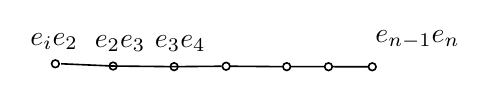
\begin{tikzpicture}[line width=.58pt,x=.52cm,y=.52cm,every node/.style={inner sep=1pt}]
\draw (.14,0)--(1.41,-.055)--(2.90,-.07)--(4.06,-.06);
\draw (4.27,-.06)--(5.54,-.07);
\draw (5.76,-.07)--(6.56,-.071);
\draw (6.78,-.071)--(7.63,-.073);
\foreach \x/\y in {0/0,1.41/-.055,2.90/-.07,4.17/-.06,5.65/-.07,6.67/-.071,7.74/-.073}
  \draw (\x,\y) circle (.093);
\node at (-.03,.54) {\(e_i e_2\)};
\node at (1.58,.50) {\(e_2e_3\)};
\node at (3.05,.50) {\(e_3e_4\)};
\node[anchor=west] at (7.73,.59) {\(e_{n-1}e_n\)};
\end{tikzpicture}}\endgroup\par
В первой подписи нижний знак с точкой прочитан как \(i\). Наконечники стрелок на цепочке не различимы.}
\end{GelfandAdjacentEvidence}
\begin{GelfandAdjacentEvidence}{GELFAND-P000860}{3}


если соед. стрелкой, то произв. \(=0\), если не соед., то новый элемент.
Идея: есть алг. типа Грассмана, но другие.
\begin{center}— \(\cdot\) —\end{center}

оператор в \(L\):
\Unclear{GELFAND-P000860}{operator-intro}{У правого конца \(L\) тёмный штрих. Самостоятельный нижний знак не установлен.}
\end{GelfandAdjacentEvidence}
\begin{GelfandAdjacentEvidence}{GELFAND-P000860}{4}

\[
A=\begin{pmatrix}A_{11}&A_{12}\\ A_{21}&A_{22}\end{pmatrix}.\tag{3}
\]
Градуировка:

[зачёркнуто: \sout{…}]
\Incomplete{GELFAND-P000860}{grading-cancellation}{Знак перед первой матрицей зачёркнут. Возможно, это \(A\).}
\end{GelfandAdjacentEvidence}
\begin{GelfandAdjacentEvidence}{GELFAND-P000860}{5}

\SourceFigure{GELFAND-P000860}{grading-labels}{%
\begingroup\color{black}\GelfandFitDiagram{\begin{tikzpicture}[line width=.54pt,every node/.style={inner sep=1pt}]
\node at (-1.55,.10) {(4)};
\node (even) at (0,0) {\(\begin{pmatrix}A_{11}&0\\0&A_{22}\end{pmatrix}\)};
\node (odd) at (2.62,-.08) {\(\begin{pmatrix}0&A_{12}\\ A_{21}&0\end{pmatrix}\)};
\draw (-.23,-.80)--(-.23,-.99);
\draw (2.66,-.84)--(2.62,-1.02);
\node[anchor=west] at (-.46,-1.20) {0-я комп.};
\node[anchor=west] at (2.33,-1.22) {1-я комп.};
\end{tikzpicture}}\endgroup}
\end{GelfandAdjacentEvidence}
\begin{GelfandAdjacentEvidence}{GELFAND-P000860}{6}

\Unclear{GELFAND-P000860}{grading-matrix-odd}{Нижний левый блок во второй матрице прочитан как \(A_{21}\).}
\end{GelfandAdjacentEvidence}
\begin{GelfandAdjacentEvidence}{GELFAND-P000860}{7}


Пр-во \(L_{p,q}\) — все такие опер., \(p=\dim L_0\), \(q=\dim L_1\).

\(L_{p,q}(\Lambda)\) — грассм. оболочка:

\uline{Замечание}: \(a_i\) и \(e_i\) всегда счит. коммутирующими.

\(L_{p,q}(\Lambda)\) — тоже матрицы из грассм. чисел:

в \(A_{11},A_{22}\) чётные
\Unclear{GELFAND-P000860}{even-block-indices}{Первый из двух индексов сильно обведён и предположительно читается как \(11\). Во втором читается \(22\).}
\end{GelfandAdjacentEvidence}


в \(A_{12},A_{21}\) нечётные.


\Needspace{7\baselineskip}
\begin{GelfandAdjacentEvidence}{GELFAND-P000861}{1}
\SourcePage{GELFAND-P000861}{unlabelled}
\[
A=\begin{pmatrix}A_{11}&A_{12}\\A_{21}&A_{22}\end{pmatrix}\in L_{p,q}(\Lambda).
\]
\(L_{p,q}(\Lambda)\) — \uline{это алгебра} (и \(\Lambda_0\)-модуль).

Суперслед
\[
\operatorname{str} A=\operatorname{tr} A_{11}-\operatorname{tr} A_{22}.\tag{5}
\]
Св-во:
\[
\operatorname{str}(AB)=\operatorname{str}(BA)\tag{6}
\]
\uwave{Супердетерминант}. (Березиниан):
\[
\operatorname{sdet}=\det(A_{11}-A_{12}A_{22}^{-1}A_{21})(\det A_{22})^{-1}\tag{7}
\]
(для числовых матриц есть ф-ла [зачёркнуто: \sout{…}] такая же, но с
\(\det A_{22}\) вместо \((\det A_{22})^{-1}\)).
\Incomplete{GELFAND-P000861}{cancelled-word}{Запись после «ф-ла» зачёркнута и не читается.}
\end{GelfandAdjacentEvidence}
\begin{GelfandAdjacentEvidence}{GELFAND-P000861}{2}

\[
\operatorname{sdet}(\alpha_1\alpha_2)=
\operatorname{sdet}\alpha_1\cdot\operatorname{sdet}\alpha_2\tag{8}
\]
\Unclear{GELFAND-P000861}{product-symbols}{Знаки в (8) предварительно переданы как \(\alpha_1,\alpha_2\). Возможно, это курсивные прописные \(A_1,A_2\).}
\end{GelfandAdjacentEvidence}
\begin{GelfandAdjacentEvidence}{GELFAND-P000861}{3}


\uline{Упражнение}. Сделать это, если \(\dim L_0=\dim L_1=1\), т.е. для матриц 2-го порядка.

\uwave{Пояснение}. Рассм. матрицы с антикоммут. элементами:
\[
\operatorname{sdet}\begin{pmatrix}1&\xi_1\\\xi_2&1\end{pmatrix}
 =1-\xi_1\xi_2.
\]
\[
\begin{pmatrix}1&\xi_1\\\xi_2&1\end{pmatrix}^{2}
=\begin{pmatrix}1+\xi_1\xi_2&2\xi_1\\2\xi_2&1+\xi_2\xi_1\end{pmatrix}.
\]
\SourceFigure{GELFAND-P000861}{post-matrix-mark}{%
\begingroup\color{black}\GelfandFitDiagram{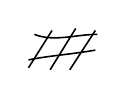
\begin{tikzpicture}[line width=.57pt,x=.025cm,y=-.025cm]
\draw (10,12) .. controls (20,16) and (31,12) .. (42,12);
\draw (7,25) .. controls (16,23) and (30,22) .. (41,20);
\draw (7,29)--(19,10);
\draw (18,30)--(31,9);
\draw (28,30)--(41,10);
\end{tikzpicture}}\endgroup\par
Справа от матрицы небольшой знак, похожий на решётку. Его назначение не установлено.}
\end{GelfandAdjacentEvidence}
\begin{GelfandAdjacentEvidence}{GELFAND-P000861}{4}

\[
\begin{aligned}
\operatorname{sdet}
 &=(1+\xi_1\xi_2-2\xi_1(1+\xi_1\xi_2)2\xi_2)(1+\xi_1\xi_2)=\\
 &=(1-3\xi_1\xi_2)(1+\xi_1\xi_2)=1-2\xi_1\xi_2=(1-\xi_1\xi_2)^2.
\end{aligned}
\]
\Unclear{GELFAND-P000861}{sdet-calc-first}{В первом произведении после \(1+\) первый нижний индекс обведён и прочитан как \(1\).}
\end{GelfandAdjacentEvidence}
\begin{GelfandAdjacentEvidence}{GELFAND-P000861}{5}


\uwave{Привед. матриц к кан. виду.}

\(L(\Lambda)\)
\Unclear{GELFAND-P000861}{faded-fragment}{Отдельная выцветшая запись предварительно прочитана как \(L(\Lambda)\).}
\end{GelfandAdjacentEvidence}
\begin{GelfandAdjacentEvidence}{GELFAND-P000861}{6}


Имеется отображение
\[
m.\quad L(\Lambda)\longrightarrow L_0
\]
\[
\begin{aligned}
\sum a_i e_i
&\longmapsto\left.\left(\sum a_i e_i\right)\right|_{\xi=0}
=\sum_i m(a_i)e_i,\\
&m(a_i)=\left.a_i\right|_{\xi=0}.
\end{aligned}
\]
\Incomplete{GELFAND-P000861}{cancelled-sum-index}{Нижняя запись при последней сумме зачёркнута. Над знаком виден неразобранный штрих.}
\end{GelfandAdjacentEvidence}
\begin{GelfandAdjacentEvidence}{GELFAND-P000861}{7}

\[
A=\begin{pmatrix}A_{11}&A_{12}\\A_{21}&A_{22}\end{pmatrix}\in L_{p,q}(\Lambda).
\]
\Unclear{GELFAND-P000861}{lower-matrix-space}{Начертание \(L\) во второй строке с матрицей прерывается. Выражение предварительно прочитано как \(L_{p,q}(\Lambda)\).}
\end{GelfandAdjacentEvidence}

\[
m(A)=\begin{pmatrix}a_1&0\\0&a_2\end{pmatrix}.\tag{9}
\]
Пусть \(\mathbb K=\mathbb C\).

\uline{Теорема}.

Пусть \(m(A)\) имеет разл. соб. знач.. Тогда \(A\) тоже прив. к диаг. виду:
\[
BAB^{-1}=\begin{pmatrix}c_1&&0\\&\ddots&\\0&&c_{p+q}\end{pmatrix}.\tag{10}
\]


\Needspace{7\baselineskip}
\begin{GelfandAdjacentEvidence}{GELFAND-P000862}{1}
\SourcePage{GELFAND-P000862}{11}
\uwave{Аналоги жорд. клеток здесь неизвестны.}

\uline{Задача 1}. \uwave{Сделать это} (\uwave{аналог норм. форм})!

Задача, имеющая отношение к инстантонам:

\uline{Задача 2}. Рассм. матрицу \(A=(a_{ik})_{i,k=1}^{n}\) с элементами
\(a_{ik}\in\Lambda_1\) (неч. гр. числа).

Описать все \(B=(b_{ik})_{i,k=1}^{n}\), с элем. \(b_{ik}\in\Lambda_0\) и такие что
\[
\underline{\underline{AB=BA}}.
\]
Если \(\Lambda\) имеет 4 образующих, то имеет отн. к Я.-М.
Если все элем. \(A\) независимы (в \(\Lambda\)), то решается.
\begin{center}— \(\cdot\) —\end{center}

\uuline{С.Г.} Связь с раб. Бейлинсона и Берншт.-Гельф.-Гельф.

(см. ФА, 1978, \(N=3\)?; или Дринфельд, Манин; Яд. физика, \(N=6\), 1979:
там явно указ. констр., перев. на язык решений).
\Unclear{GELFAND-P000862}{reference-issue}{Знак вопроса после \(N=3\) имеется в рукописи.}
\end{GelfandAdjacentEvidence}
\begin{GelfandAdjacentEvidence}{GELFAND-P000862}{2}


\uwave{классиф. вект. рассл.} на \(\mathbb C P^3\). (голом.)

Объекты — град. модули над \(\Lambda=\Lambda(4)\):
\SourceFigure{GELFAND-P000862}{graded-chain}{%
\begingroup\color{black}\GelfandFitDiagram{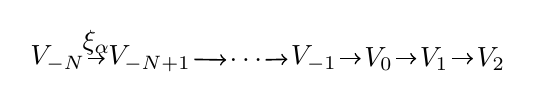
\begin{tikzpicture}[line width=.59pt,x=.72cm,y=.72cm,every node/.style={inner sep=1pt}]
\node (a) at (0,0) {\(V_{-N}\)};
\node (b) at (1.62,0) {\(V_{-N+1}\)};
\node (c) at (3.32,-.03) {\(\ldots\)};
\node (d) at (4.52,0) {\(V_{-1}\)};
\node (e) at (5.66,0) {\(V_0\)};
\node (f) at (6.64,0) {\(V_1\)};
\node (g) at (7.64,0) {\(V_2\)};
\draw[->] (a)--node[above] {\(\xi_\alpha\)} (b);
\draw[->] (b)--(c);
\draw[->] (c)--(d);
\draw[->] (d)--(e);
\draw[->] (e)--(f);
\draw[->] (f)--(g);
\end{tikzpicture}}\endgroup}
\end{GelfandAdjacentEvidence}
\begin{GelfandAdjacentEvidence}{GELFAND-P000862}{3}

\(\alpha=1,2,3,4\). \quad Предст. грассм. алгебры:
\[
\xi_i\xi_j+\xi_j\xi_i=0.
\]
\(a_1\xi_1+a_2\xi_2+a_3\xi_3+a_4\xi_4\) — оператор из \(V_k\) в \(V_{k+1}\)

и получ. \uline{комплекс};

когом. нулевые, кроме \(H^0\).

Такие модули с точн. до трив. классифицируют инстантоны.
\Unclear{GELFAND-P000862}{module-equivalence}{Сокращение после «до» предварительно читается «трив.».}
\end{GelfandAdjacentEvidence}
\begin{GelfandAdjacentEvidence}{GELFAND-P000862}{4}


\dashuline{Задача}: дать явную конструкцию. Не сделано (строятся пр-ва, но не отображения).

\dashuline{Задача}: \uwave{сделать классиф. для грассманова мн-зия}!!

\uuline{Ю. Шабат.}
\Unclear{GELFAND-P000862}{speaker-initial}{В рукописи инициал «Ю.». В \href{https://old.mccme.ru/gelfand/notes/record-469.html}{записи 469 каталога МЦНМО} имя указано как «G.B. Shabat».}
\end{GelfandAdjacentEvidence}
\begin{GelfandAdjacentEvidence}{GELFAND-P000862}{5}


\uline{Теорема Ли–Виртингера} (классическая)

\(\Gamma\subset\mathbb C^n\) — росток аналитич. гиперповерхности.
Она наз. \uwave{двойной пов. переноса}, если она 2-мя спос. предст. в виде суммы
\[
\Gamma=\gamma_1+\ldots+\gamma_{n-1},
\qquad
\Gamma=\delta_1+\ldots+\delta_{n-1}
\]
\(\gamma_i,\delta_i\) — ростки аналит. кривых.

\(\{\gamma_i\}\) и \(\{\delta_i\}\) не получ. друг из друга перест.
[зачёркнуто: \sout{…}] и сдвигами.
\Incomplete{GELFAND-P000862}{cancelled-qualifier}{Запись после «перест.» зачёркнута и не читается.}
\end{GelfandAdjacentEvidence}


\uline{Пример}: \(X\) — гладкая кривая рода \(n\).

\(JX\) — якобиан кривой \(X\); \quad \(j:X\longrightarrow JX\).


\Needspace{7\baselineskip}
\begin{GelfandAdjacentEvidence}{GELFAND-P000863}{1}
\SourcePage{GELFAND-P000863}{unlabelled}
\[
\Theta=\underbrace{j(X)+\ldots+j(X)}_{n-1\text{ раз}},
\qquad (\Theta\text{ — дивизор Пуанкаре}).
\]
По теор. Римана он симм., т.е. \(\exists K\in JX\):
\[
\Theta=K-\Theta.
\]
\Unclear{GELFAND-P000863}{riemann-constant}{В обоих местах знак передан как \(K\). Возможное чтение — \(\kappa\).}
\end{GelfandAdjacentEvidence}
\begin{GelfandAdjacentEvidence}{GELFAND-P000863}{2}


Поэтому с точн. до сдвига
\[
\Theta\sim\underbrace{-jX-\ldots-jX}_{n-1}.
\]
Пусть \(X\ne-jX\) (\(\Leftrightarrow X\) не гиперэллиптична).
\Unclear{GELFAND-P000863}{embedded-curve}{Слева в рукописи стоит \(X\) без \(j\).}
\end{GelfandAdjacentEvidence}
\begin{GelfandAdjacentEvidence}{GELFAND-P000863}{3}


\uline{Утвержд.}: все пов. переноса — эти пов. и их вырождения

(если \(\Gamma\) — дв. пов. переноса, то малая деформ. \(\Gamma\) — росток \(\Theta\subset JX\)).

\uline{Гипотеза И.М.Г.}: 1) Все интегр. системы имеют в основе эту теорему.

2) Эта теор. — первая в ряду колосал. теорем такого вида.
\Unclear{GELFAND-P000863}{hypothesis-word}{Сокращение предварительно читается «колосал.». Средние штрихи слиты.}
\end{GelfandAdjacentEvidence}
\begin{GelfandAdjacentEvidence}{GELFAND-P000863}{4}


1) — причина появл. \(\Theta\)-ф-й.
\begin{center}— \(\cdot\) —\end{center}

\uuline{Höegh-Krohn?} \quad \uuline{некто из Норвегии.} (в переводе Гельфанда).
\Unclear{GELFAND-P000863}{speaker-name}{В рукописи после имени стоит вопросительный знак. В \href{https://old.mccme.ru/gelfand/notes/record-470.html}{записи 470 каталога МЦНМО} указано «Raphael Hoegh-Krohn».}
\end{GelfandAdjacentEvidence}
\begin{GelfandAdjacentEvidence}{GELFAND-P000863}{5}


О группах отобр.

(Исмагилов, Граев, Вершик; Albeverio)

[под списком: и \ldots]

\(X\) — рим. мн-зие

\(G\) — комп. гр. Ли (простая)
\[
\varphi\in C_0^\infty(X,G)\equiv G^X.
\]
\Unclear{GELFAND-P000863}{mapping-letter}{Знак с открытой петлёй передан как \(\varphi\). Возможное чтение — \(\psi\).}
\end{GelfandAdjacentEvidence}
\begin{GelfandAdjacentEvidence}{GELFAND-P000863}{6}

Изучаем унит. представления.

\(g\) — алг. Ли \(G\).

[слева зачёркнуто: \sout{…}] \(\Omega(X,g)\) — 1-формы со знач. в алг. Ли.
\Incomplete{GELFAND-P000863}{cancelled-form-prefix}{Знак перед \(\Omega(X,g)\) зачёркнут и не читается.}
\end{GelfandAdjacentEvidence}
\begin{GelfandAdjacentEvidence}{GELFAND-P000863}{7}

\[
\omega_i\in\Omega(X,g)
\]
\[
(\omega_1,\omega_2)=\int_X\operatorname{tr}\bigl(\omega_1(x)\omega_2^*(x)\bigr)\,dx.\tag{1}
\]
\Unclear{GELFAND-P000863}{cancelled-star}{Тёмный штрих над \(\omega_1\) может быть зачёркнутой звёздочкой. Точное чтение не установлено.}
\end{GelfandAdjacentEvidence}
\begin{GelfandAdjacentEvidence}{GELFAND-P000863}{8}

\[
\omega_i(x):T_x\longrightarrow g
\]
в обоих пр-вах есть ск. пр. (справа — Киллинг)

\SourceFigure{GELFAND-P000863}{adjoint-identification}{%
\begingroup\color{black}\GelfandFitDiagram{\begin{tikzpicture}[line width=.6pt,every node/.style={inner sep=1pt}]
\node[anchor=east] at (-.72,.72) {\(\omega_2^*(x):\)};
\node (txdual) at (0,.72) {\(T_x^*\)};
\node (gdual) at (1.50,.72) {\(g^*\)};
\draw[->] (gdual.west)--(txdual.east);
\draw (-.06,.38)--(-.10,.03) (.06,.38)--(.02,.03);
\draw (1.45,.33)--(1.42,.06) (1.54,.33)--(1.51,.06);
\node at (0,-.22) {\(T_x\)};
\node at (1.49,-.13) {\(g\)};
\node[anchor=west] at (2.01,.18) {— отожд.};
\end{tikzpicture}}\endgroup}
\end{GelfandAdjacentEvidence}



\Needspace{7\baselineskip}
\begin{GelfandAdjacentEvidence}{GELFAND-P000864}{1}
\SourcePage{GELFAND-P000864}{12}
\[
\omega_1\omega_2^*:g\longrightarrow g
\]
след и интегр. берутся теперь

\(\mathcal H\) — гильб. пр-во, пополн. \(\Omega(X,g)\)
\[
L_2(\mathcal H,\mu)
\]
\[
\dim\mathcal H<\infty\quad\Rightarrow\quad d\mu\sim e^{-\frac12|x|^2}\,dx
\]
\Unclear{GELFAND-P000864}{finite-dimension-sign}{Знак \(\infty\) обведён повторно. Под ним виден отдельный штрих.}
\end{GelfandAdjacentEvidence}
\begin{GelfandAdjacentEvidence}{GELFAND-P000864}{2}

(и аналог. в [зачёркнуто: \sout{конечно}] \(\infty\)-мерн. пр-ве)
\Unclear{GELFAND-P000864}{cancelled-word}{Зачёркнутое слово предварительно читается «конечно».}
\end{GelfandAdjacentEvidence}
\begin{GelfandAdjacentEvidence}{GELFAND-P000864}{3}


\(T\in E(\mathcal H)\) — евклид. преобр. (движения) пр-ва \(\mathcal H\),
\[
Tx=Ox+a,\qquad x\in H,\quad a\in H
\]
\(\mu\) инвар. отн. \(O\) и квазиинв. отн. переносов.

\(g\in E(\mathcal H)\), \(g\to U_g\) унит. на \(L_2(\mathcal H,\mu)\)

отсюда ср. унит. предст. \(E(\mathcal H)\) в \(L_2(\mathcal H,\mu)\)
\Unclear{GELFAND-P000864}{representation-abbrev}{Сокращение предварительно передано как «ср.». Второй знак имеет длинный нисходящий штрих.}
\end{GelfandAdjacentEvidence}
\begin{GelfandAdjacentEvidence}{GELFAND-P000864}{4}

\[
(\alpha(\varphi)\omega)(x)=\operatorname{Ad}\varphi(x)\,\omega(x)
+\varphi^{-1}(x)\,d\varphi(x).\tag{2}
\]
\Unclear{GELFAND-P000864}{mapping-letter}{Знак с открытой петлёй передан как \(\varphi\). Возможное чтение — \(\psi\).}
\end{GelfandAdjacentEvidence}
\begin{GelfandAdjacentEvidence}{GELFAND-P000864}{5}

\Unclear{GELFAND-P000864}{affine-law}{В рукописи видны порядок \(\varphi^{-1}(x)\,d\varphi(x)\) и степень \(-1\).}
\end{GelfandAdjacentEvidence}
\begin{GelfandAdjacentEvidence}{GELFAND-P000864}{6}

\[
\alpha:C_0^\infty(X,G)\longrightarrow E(\Omega(X))
\]
— это гомоморфизм групп:
\[
\alpha(\varphi_1\varphi_2)=\alpha(\varphi_1)\alpha(\varphi_2).
\]
Берем композ. с \(U_g\);
\[
\underline{\underline{V_\phi=U_{\alpha(\phi)}}}
\quad\text{— получ. унит. предст.}
\]
\Unclear{GELFAND-P000864}{boxed-map-letters}{В подчёркнутой формуле петли имеют иное начертание. Здесь они переданы через \(\phi\).}
\end{GelfandAdjacentEvidence}

\[
\varphi\longrightarrow V_\varphi.
\]
\uline{Теорема 1}. Оно неприводимо, если \(\dim X\geq 3\).
\[
\begin{aligned}
\geq5&\text{ — Исмагилов}\\
\geq4&\text{ — Гельф., Граев, Вершик}\\
\geq3&\text{ — Альбеверио и Хёг-Крон.}
\end{aligned}
\]
\uline{Теорема 2}. \(\dim X=1\quad\Rightarrow\) предст. приводимо
\[
\underline{\dim X=2}\qquad\text{— ?}
\]
\(b(t)\) — броун. дв-ние в \(g\). (стандартное; по отн. к форме Киллинга)

Рассм. ур-е
\[
\eta^{-1}(t)\,d\eta(t)=db(t),\qquad
\eta\in C(\mathbb R^+,G).\tag{3}
\]


\Needspace{7\baselineskip}
\begin{GelfandAdjacentEvidence}{GELFAND-P000865}{1}
\SourcePage{GELFAND-P000865}{unlabelled}
Объяснение:

\(b(t)\) — мера на \(C_0(\mathbb R^+,g)\) — обозначим её \(\mu_0\).
\[
b(t)\in\bigl(C_0(\mathbb R^+,g),\mu\bigr)
\]
Реш. обычное ур-е
 
Получ. отобр.
\[
\bigl(C(\mathbb R^+,G),\mu_0\bigr)\longrightarrow C(\mathbb R^+,G)
\]
\Unclear{GELFAND-P000865}{path-measure-notation}{В первой формуле стоит \(C_0(\mathbb R^+,g)\) с \(\mu\), а в области отображения — \(C(\mathbb R^+,G)\) с \(\mu_0\).}
\end{GelfandAdjacentEvidence}
\begin{GelfandAdjacentEvidence}{GELFAND-P000865}{2}


Стохастич. — решить и перенести меру.
\[
\eta(t)\longrightarrow\phi(t)\eta(t);
\]
\Unclear{GELFAND-P000865}{mapping-letter}{В этих двух формулах буква с замкнутой петлёй предварительно передана как \(\phi\).}
\end{GelfandAdjacentEvidence}
\begin{GelfandAdjacentEvidence}{GELFAND-P000865}{3}

\[
\frac{d\mu(\phi\eta)}{d\mu(\eta)}
\]
\SourceFigure{GELFAND-P000865}{nationality-insertions}{%
\begingroup\color{black}\GelfandFitDiagram{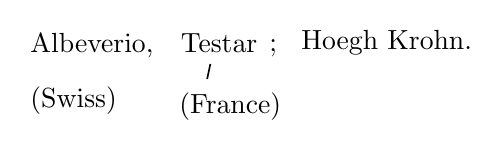
\begin{tikzpicture}[line width=.59pt,every node/.style={inner sep=1pt}]
\node[anchor=west] at (0,.63) {Albeverio,};
\node[anchor=west] at (1.91,.65) {Testar};
\node at (3.13,.59) {;};
\node[anchor=west] at (3.44,.66) {Hoegh Krohn.};
\node[anchor=west] at (0,-.07) {(Swiss)};
\draw (2.33,.39)--(2.29,.20);
\node[anchor=west] at (1.89,-.15) {(France)};
\end{tikzpicture}}\endgroup}
\end{GelfandAdjacentEvidence}
\begin{GelfandAdjacentEvidence}{GELFAND-P000865}{4}

\Unclear{GELFAND-P000865}{latin-name}{Первое имя предварительно прочитано «Albeverio». Второе читается «Testar». В более поздней \href{https://doi.org/10.1016/0022-1236(81)90082-3}{статье 1981 года} имена напечатаны как S. Albeverio, R. Høegh-Krohn и D. Testard.}
\end{GelfandAdjacentEvidence}
\begin{GelfandAdjacentEvidence}{GELFAND-P000865}{5}

\[
L_2\bigl(C(\mathbb R^+,G),\mu\bigr),\qquad
\varphi\in C^\infty(\mathbb R^+,G)
\]
\Unclear{GELFAND-P000865}{mapping-letter-open}{В строке с \(C^\infty\) открытая петля передана как \(\varphi\).}
\end{GelfandAdjacentEvidence}

\[
\eta\longrightarrow\varphi\eta
\]
\(\varphi\longrightarrow W_\varphi\) \quad получ. унит. предст. на \(L_2(C(\mathbb R^+,G),\mu)\)

\uline{Теорема} \(W_\varphi\cong V_\varphi\) \quad эквивалентны.

Соотв. коцикл — форма Маурера–Картана.

Факторы:
\[
[L_\infty\cup W_\varphi]''\qquad\text{— фактор типа 3.}
\]


\Needspace{7\baselineskip}
\begin{GelfandAdjacentEvidence}{GELFAND-P000866}{1}
\SourcePage{GELFAND-P000866}{unlabelled}
\uuline{22.10.79 г.} \qquad \uuline{Сем. Гельфанда.}

\uline{Некто.} (\uuline{Батурин})
\Unclear{GELFAND-P000866}{speaker-name}{Рукописное имя предварительно прочитано «Батурин». В \href{https://old.mccme.ru/gelfand/notes/record-471.html}{записи 471 каталога МЦНМО} указано «I.A. Batalin».}
\end{GelfandAdjacentEvidence}
\begin{GelfandAdjacentEvidence}{GELFAND-P000866}{2}


\uline{О связях.}

\uwave{Связи 1-го рода}
\[
\begin{aligned}
H&\text{ — гамильтониан},\qquad T_\alpha\text{ — связи}\\
H,T_\alpha&\text{ — ф-и от }q\text{ и }p.
\end{aligned}\tag{1}
\]
\[
\{T_\alpha,T_\beta\}=u_{\alpha\beta}^{\gamma}T,\qquad
g^a=\begin{pmatrix}q^i\\p_i\end{pmatrix}.\tag{2}
\]
\Unclear{GELFAND-P000866}{constraint-index}{После \(u_{\alpha\beta}^{\gamma}\) у \(T\) нижний индекс не виден.}
\end{GelfandAdjacentEvidence}
\begin{GelfandAdjacentEvidence}{GELFAND-P000866}{3}

\[
\{A,B\}=\frac{\partial A}{\partial g^a}\,\varepsilon^{ab}
\frac{\partial B}{\partial g^b},\qquad
\text{здесь }-\varepsilon^{ba}=\varepsilon^{ab}
=\begin{pmatrix}0&1\\-1&0\end{pmatrix}.\tag{3}
\]
Связи 1-го рода — если выполнено условие (2), \quad
\(u_{\alpha\beta}^{\gamma}=u_{\alpha\beta}^{\gamma}(p,q)\).
\[
\text{\uline{Вопрос}:}\quad
\text{можно ли сделать заменами пер., чтобы было}\quad u_{\alpha\beta}^{\gamma}=\mathrm{const}.\tag{4}
\]
\uline{Замеч. о мотивировке}: калибр. преобр. генерир. только связями 1-го рода

\uwave{Действие}:
\[
S=\int dt\left[\frac12 g^a\varepsilon_{ab}\dot g^b-H-\lambda^\alpha T_\alpha\right].\tag{5}
\]
(\(\lambda^\alpha\) — обычные переменные;
[зачёркнуто: \sout{…}] экстремум теперь безусловный)
\Incomplete{GELFAND-P000866}{cancelled-extremum}{Запись перед «экстремум» зачёркнута и не читается.}
\end{GelfandAdjacentEvidence}
\begin{GelfandAdjacentEvidence}{GELFAND-P000866}{4}


Калибр. преобр. генерир. связями
 
[ниже зачёркнуто: \sout{\(g^a\quad\delta g^a=\cdots\)}]
\Unclear{GELFAND-P000866}{cancelled-coordinate}{Под штриховкой предварительно читаются \(g^a\) и \(\delta g^a=\). Конец не читается.}
\end{GelfandAdjacentEvidence}
\begin{GelfandAdjacentEvidence}{GELFAND-P000866}{5}

\begin{center}— \(\bullet\) —\end{center}

\uuline{Р. Каллош.} \qquad \uline{Квантовая теория поля}

[зачёркнута строка: \sout{\((1)\quad\Delta\phi_l=\lambda_l\phi_l,\ \ldots\)}]
\Unclear{GELFAND-P000866}{cancelled-eigen-equation}{Левая часть зачёркнутой строки предположительно читается \((1)\quad\Delta\phi_l=\lambda_l\phi_l\). Индексы не вполне ясны.}
\end{GelfandAdjacentEvidence}
\begin{GelfandAdjacentEvidence}{GELFAND-P000866}{6}

\Incomplete{GELFAND-P000866}{cancelled-equation-right}{Правая часть после запятой густо заштрихована и не читается.}
\end{GelfandAdjacentEvidence}
\begin{GelfandAdjacentEvidence}{GELFAND-P000866}{7}


\uwave{Новые Ноб. лауреаты}
\SourceFigure{GELFAND-P000866}{weak-interactions}{%
\begingroup\color{black}\GelfandFitDiagram{\begin{tikzpicture}[every node/.style={inner sep=1pt,anchor=west}]
\node at (0,.52) {\uwave{Вайнберг, Глэшоу, Салам} —};
\node at (1.22,-.01) {за слабые взаимод.};
\end{tikzpicture}}\endgroup}
\end{GelfandAdjacentEvidence}
\begin{GelfandAdjacentEvidence}{GELFAND-P000866}{8}


В основе всего — симметрия. Рассм. конт. интеграл.
\[
e^{iW[\varphi]}=\int d\phi\cdot\exp\{iS[\phi,\varphi]\}.\tag{1}
\]
\Unclear{GELFAND-P000866}{field-letter}{Открытая петля передана как \(\varphi\) (возможно, \(\psi\)). Замкнутая петля переменной интегрирования передана как \(\phi\).}
\end{GelfandAdjacentEvidence}
\begin{GelfandAdjacentEvidence}{GELFAND-P000866}{9}

\Incomplete{GELFAND-P000866}{cancelled-action-index}{Знак под \(S\) замаран и не читается.}
\end{GelfandAdjacentEvidence}
\begin{GelfandAdjacentEvidence}{GELFAND-P000866}{10}


\(S\) строится по класс. действию

по (1) многое опред.: вероятности, \(S\)-матрице.
\Unclear{GELFAND-P000866}{scattering-term}{Последняя буква в слове «матрице» предварительно прочитана как «е».}
\end{GelfandAdjacentEvidence}
\begin{GelfandAdjacentEvidence}{GELFAND-P000866}{11}


\(\phi\) — квантовые флукт. (по ним усредняют)

\(S\)-матрица
\[
S[\varphi_{in}]=e^{iW[\widetilde{\varphi}[\varphi_{in}]]},\tag{2}
\]
\SourceFigure{GELFAND-P000866}{scattering-insertion}{%
\begingroup\color{black}\GelfandFitDiagram{\begin{tikzpicture}[line width=.55pt,every node/.style={inner sep=1pt}]
\node at (0,.70) {\(\varphi_{in}\)};
\draw (-.11,.42)--(-.18,.20);
\node[anchor=west] at (-.49,.02) {своб. поля на \(\infty\).};
\end{tikzpicture}}\endgroup}
\end{GelfandAdjacentEvidence}



\Needspace{7\baselineskip}
\begin{GelfandAdjacentEvidence}{GELFAND-P000867}{1}
\SourcePage{GELFAND-P000867}{unlabelled}
\begin{equation*}
\widetilde{\varphi}=\varphi_{in}
+\int D^c(x-x')\frac{\delta\mathcal{L}_{int}}{\delta\widetilde{\varphi}(x')}\,d^4x'. \tag{3}
\end{equation*}
\Unclear{GELFAND-P000867}{field-letter}{Петлеобразный знак в (3) и на рисунке передан как $\varphi$ (возможно, $\psi$).}
\end{GelfandAdjacentEvidence}
\begin{GelfandAdjacentEvidence}{GELFAND-P000867}{2}


(ур-е Янга--Фельдмана)

Итерац. реш. (3) даёт деревья.

$D^c$ --- ф-я Грина своб. ур-я Кл.-Гордона.

\SourceFigure{GELFAND-P000867}{tree-diagram}{%
\begingroup\color{black}\GelfandFitDiagram{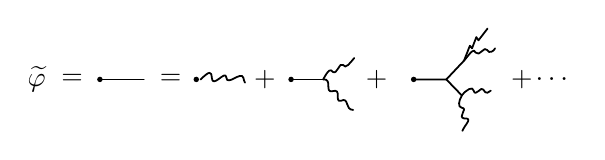
\begin{tikzpicture}[x=.68cm,y=.68cm,line width=.64pt,line cap=round,line join=round]
\node[inner sep=0pt] at (0,0) {$\widetilde{\varphi}$};
\node at (.66,0) {$=$};
\foreach \x in {1.18,2.98,4.75,7.04}
  \fill (\x,0) circle (.051);
\draw (1.18,0)--(2.00,0);
\node at (2.50,0) {$=$};
\draw (3.06,0)
  .. controls (3.23,.16) and (3.26,.16) .. (3.27,.03)
  .. controls (3.28,-.18) and (3.53,.19) .. (3.54,.04)
  .. controls (3.55,-.14) and (3.82,.17) .. (3.86,.03)
  .. controls (3.87,.00) and (3.87,-.04) .. (3.89,-.06);
\node at (4.26,0) {$+$};
\draw (4.75,0)--(5.35,0);
\draw (5.35,0)
  .. controls (5.45,.19) and (5.49,.20) .. (5.53,.14)
  .. controls (5.61,.08) and (5.66,.34) .. (5.72,.27)
  .. controls (5.77,.18) and (5.86,.32) .. (5.93,.40);
\draw (5.35,0)
  .. controls (5.53,.02) and (5.37,-.25) .. (5.52,-.22)
  .. controls (5.71,-.16) and (5.55,-.43) .. (5.68,-.40)
  .. controls (5.84,-.32) and (5.75,-.57) .. (5.91,-.57);
\node at (6.35,0) {$+$};
\draw (7.04,0)--(7.65,0)--(7.98,.35);
\draw (7.65,0)--(7.94,-.30);
\draw (7.98,.35)--(8.09,.63)--(8.13,.58)--(8.21,.79)
  --(8.25,.73)--(8.42,.95);
\draw (7.98,.35)
  .. controls (8.10,.49) and (8.16,.60) .. (8.20,.50)
  .. controls (8.26,.41) and (8.37,.64) .. (8.41,.55)
  .. controls (8.45,.47) and (8.54,.53) .. (8.56,.58);
\draw (7.94,-.30)
  .. controls (8.02,-.19) and (8.15,-.12) .. (8.16,-.21)
  .. controls (8.19,-.34) and (8.31,-.11) .. (8.34,-.19)
  .. controls (8.39,-.29) and (8.45,-.24) .. (8.48,-.21);
\draw (7.94,-.30)
  .. controls (7.88,-.40) and (7.86,-.52) .. (7.94,-.53)
  .. controls (8.07,-.54) and (7.84,-.71) .. (7.99,-.73)
  .. controls (8.15,-.72) and (8.00,-.84) .. (7.95,-.96);
\node at (9.06,0) {$+$};
\node at (9.62,0) {$\ldots$};
\end{tikzpicture}}\endgroup}
\end{GelfandAdjacentEvidence}
\begin{GelfandAdjacentEvidence}{GELFAND-P000867}{3}


В ф-ле (2) есть амплитуды рожд. любого числа частиц.

Для гравитации

\Unclear{GELFAND-P000867}{cancelled-action-sign}{Перед $S_{\text{кл}}$ зачёркнут знак, возможно $\mathcal L$.}
\end{GelfandAdjacentEvidence}
\begin{GelfandAdjacentEvidence}{GELFAND-P000867}{4}

\begin{equation*}
S_{\text{кл}}=\int\mathcal{L}\,d^4x,\qquad
\mathcal{L}=\sqrt{g}\,R[g_{\mu\nu}]. \tag{4}
\end{equation*}

$S$ в (1) отлич. кв. поправками
\begin{equation*}
\begin{array}{cc}
\varphi&g_{\mu\nu}\\
\phi&h_{\mu\nu}
\end{array} \tag{5}
\end{equation*}
\Unclear{GELFAND-P000867}{field-pair}{Верхний знак прочитан как $\varphi$ (возможно, $\psi$), нижний передан как $\phi$.}
\end{GelfandAdjacentEvidence}
\begin{GelfandAdjacentEvidence}{GELFAND-P000867}{5}

Для гравитации.
\begin{equation*}
e^{iW[g_{\mu\nu}]}=\int dh\cdot
 e^{i\{S_{\text{кл}}[g_{\mu\nu}+h_{\mu\nu}]+S_{\text{кал}}+S_{\text{ф.ч.}}\}}\,
 d\bar c\,dc. \tag{6}
\end{equation*}

ф. ч. --- \uwave{фиктивных частиц}.

$S_{\text{кл}}$ зад. ф-лой (4) и явл. ф-лом от метрики $g$.

$h_{\mu\nu}$ --- \uwave{флуктуации метрики}.
\begin{equation*}
S_{\text{кал.}}=\int\frac12
\left(D_\mu[g]h^{\mu}_{\nu}-\frac12 D_\nu[g]h_{\mu}^{\mu}\right)^2
\sqrt{g}\,d^4x. \tag{7}
\end{equation*}
\Unclear{GELFAND-P000867}{gauge-action-index}{Аргумент второго $D$ написан слитно с началом $h$ и прочитан как $[g]$.}
\end{GelfandAdjacentEvidence}
\begin{GelfandAdjacentEvidence}{GELFAND-P000867}{6}


$D_\mu$ --- ковар. произв. по метрике $g$

Подним. и опускание инд. с пом. по $g$.
\begin{equation*}
S_{\text{ф.ч.}}=\int\sqrt{g}\,\bar c^{\nu}D_\mu[g]D^{\mu}[g+h]c_\nu\,d^4x. \tag{8}
\end{equation*}

$S_{\text{ф.ч.}}$ строится по $S_{\text{кал}}$ так, чтобы ответ не зависел от $S_{\text{кал}}$

(принцип квант. относительности).

\uwave{Заметил} \underline{Фейнман}: без $S_{\text{кал}}$ нет \textcolor{orange!65!black}{[зачёркнуто]} унитарности (полная вер. $=1$)
\Unclear{GELFAND-P000867}{cancelled-unitarity}{Короткая зачёркнутая запись перед «унитарности» неразборчива.}
\end{GelfandAdjacentEvidence}
\begin{GelfandAdjacentEvidence}{GELFAND-P000867}{7}

\EvidenceBlock{GELFAND-P000867}{feynman-action-index}{В замечании рукописи написано $S_{\text{кал}}$.}{\GelfandExcerptCaption}

Он в 1-м прибл.

Де Витт, Попов, Фаддеев --- дальше.

\Unclear{GELFAND-P000867}{cancelled-bottom}{Зачёркнуто: «В … зад». Среднее сокращение, возможно «прибл.», неразборчиво.}
\end{GelfandAdjacentEvidence}


В суперграв. дост. ещё 1 члена.


\Needspace{7\baselineskip}
\begin{GelfandAdjacentEvidence}{GELFAND-P000868}{1}
\SourcePage{GELFAND-P000868}{26}
В произв. теории --- беск. число членов.

\begin{equation*}
\underset{\text{(Эйншт.)}}{S_{\text{кл}}[g]}
\qquad\text{инв. отн. преобразований}
\tag{9}
\end{equation*}
\begin{equation*}
\delta g_{\mu\nu}=D_\mu\xi_\nu+D_\nu\xi_\mu,\qquad
\xi_\mu\quad
\begin{array}{@{}l@{}}
\text{--- произв. вектор}\\[-.25ex]
\text{\phantom{--- }(лок. ф-я $x$).}
\end{array}
\tag{10}
\end{equation*}

В квантовой задаче есть инвариантность:
\begin{equation*}
W[g_{\mu\nu}]=W[g_{\mu\nu}+\delta g_{\mu\nu}],\qquad
\delta g_{\mu\nu}\text{ взято из (10)}
\tag{11}
\end{equation*}

На самом деле (6) надо ещё уточнить.

Другой закон инвариантности. Рассмотрим:
\begin{equation*}
\begin{aligned}
e^{iW_{\text{рад}}}\underset{\mathrm{def}}{=}\int dh\cdot\exp i\Bigl\{
&S_{\text{кл}}[g+h]-S_{\text{кл}}[g]
-\frac{\delta S[g]}{\delta g_{\mu\nu}}h_{\mu\nu}+{}\\
&{}+S_{\text{кал}}\bigl(F(h)\bigr)+S_{\text{ф.ч.}}\bigl(F(h)\bigr)\Bigr\}.
\end{aligned}
\tag{12}
\end{equation*}
\Unclear{GELFAND-P000868}{eq12-final}{Штрих перед $h$ обведён. Последний аргумент прочитан как $F(h)$, возможно $Fh$.}
\end{GelfandAdjacentEvidence}
\begin{GelfandAdjacentEvidence}{GELFAND-P000868}{2}


$F$ --- нек-рая функция, удовл. опр. условиям.

Калибр. преобр. [зачёркнуто] сохр. вещи, имеющие физ. смысл.
\Unclear{GELFAND-P000868}{text-cancel}{Зачёркнутое слово неразборчиво.}
\end{GelfandAdjacentEvidence}
\begin{GelfandAdjacentEvidence}{GELFAND-P000868}{3}


(Пр-во остаётся \uwave{изометричным} \uuline{старому}; пр-во старое, а коорд. меняю).

\uwave{Добавл. членов} $S_{\text{кал}},\ S_{\text{ф.ч.}}$
нужно, чтобы справиться с вырожд. при разл. по методу стац. фазы.

\begin{equation*}
W_{\text{рад}}[g_{\mu\nu}]_F
=W_{F+\delta F}[g]-\frac{\delta S[g]}{\delta g_{\mu\nu}}
\langle\delta h_{\mu\nu}\rangle
\tag{13}
\end{equation*}

$S_{\text{кал}}$ доб. для сходимости (испр. вырождения)
\[
\frac{\delta S}{\delta g_{\mu\nu}(x)\,\delta g_{\mu'\nu'}(x')}
\]
\Unclear{GELFAND-P000868}{derivative}{В числителе видно $\delta S$. Степень при $\delta$ не различима.}
\end{GelfandAdjacentEvidence}
\begin{GelfandAdjacentEvidence}{GELFAND-P000868}{4}


Вид членов, к-рые можно добавлять:
\begin{equation*}
S[\Phi]+\phi^i F_{i\alpha}\gamma^{\alpha\beta}F_{j\beta}\phi^j
\tag{14}
\end{equation*}
\Unclear{GELFAND-P000868}{fields-in-quadratic}{Оба малых знака имеют форму с двумя петлями и переданы как $\phi$, как нижний знак в (5).}
\end{GelfandAdjacentEvidence}
\begin{GelfandAdjacentEvidence}{GELFAND-P000868}{5}


Пусть внешняя метрика --- плоская
\begin{equation*}
S[\Phi]+\frac12\Phi^i F_{ij}\Phi^j
\tag{15}
\end{equation*}
\Unclear{GELFAND-P000868}{cancelled-formula}{Зачёркнута строка, прочитанная как $S[g+h]+\sum\frac12\int h^{\mu\nu}(x)$. Знак, похожий на $\sum$, пересечён линией зачёркивания.}
\end{GelfandAdjacentEvidence}



\Needspace{7\baselineskip}
\begin{GelfandAdjacentEvidence}{GELFAND-P000869}{1}
\SourcePage{GELFAND-P000869}{unlabelled}
\begin{equation*}
S[g+h]+\frac12\int h^{\mu\nu}(x)
F_{\mu\nu\mu'\nu'}(x,x',g)h^{\mu'\nu'}(x')\,d^4x\,d^4x'
\tag{16}
\end{equation*}
$F$ --- достат. произв. ф-я от точек и метрики, например:
\begin{equation*}
\frac12\left(D_\mu h^\mu_\nu-\frac\beta2D_\nu h\right)^2
\qquad\text{или}\qquad h^\mu h_\mu^\nu
\tag{17}
\end{equation*}
\Unclear{GELFAND-P000869}{eq17-alt}{После «или» написано $h^\mu h_\mu^\nu$. Нижнего индекса у первого $h$ не видно.}
\end{GelfandAdjacentEvidence}
\begin{GelfandAdjacentEvidence}{GELFAND-P000869}{2}


Принцип относит. --- от $F$ не зависит. Получилась кв. форма
\begin{equation*}
\frac12\frac{\delta^2S[g+h]}{\delta h_{\mu\nu}(x)\,\delta h_{\mu'\nu'}(x')}
+F_{\mu\nu\mu'\nu'}(x,x')
\tag{18}
\end{equation*}
Надо, чтобы получилась невыр. квадр. форма. Это условие на $F$.

Добавка в (16) --- калибр. действие.

\uwave{Читать}: Фаддеев, Попов --- обзор в УФН.

\Unclear{GELFAND-P000869}{cancelled-before13}{Зачёркнуты две записи. Первая, возможно, «Теперь». Нижняя неразборчива.}
\end{GelfandAdjacentEvidence}
\begin{GelfandAdjacentEvidence}{GELFAND-P000869}{3}

В (13):

$\langle\delta h_{\mu\nu}\rangle$ --- изменение в инт., к-рое вызывает данное изменение калибровки.
\[
\langle\delta h_{\mu\nu}\rangle=\int dh\cdot\exp i\{\widetilde S\}
\]
\Unclear{GELFAND-P000869}{average}{Правая часть заканчивается на $\exp i\{\widetilde S\}$.}
\end{GelfandAdjacentEvidence}
\begin{GelfandAdjacentEvidence}{GELFAND-P000869}{4}

\begin{equation*}
\delta h_{\mu\nu}=D_\mu\xi_\nu+D_\nu\xi_\mu,\qquad
\xi_\mu[\delta F]
\tag{19}
\end{equation*}

Выб. $F$ такое, что
\begin{equation*}
\frac12h_{\mu\nu}F_{\mu\nu\mu'\nu'}h_{\mu'\nu'}
=(h+\delta h)(F+\delta F)\cdot(h+\delta h).
\tag{20}
\end{equation*}
\Unclear{GELFAND-P000869}{eq20-factor}{Множитель $\frac12$ виден только в левой части.}
\end{GelfandAdjacentEvidence}
\begin{GelfandAdjacentEvidence}{GELFAND-P000869}{5}


По построению:
\begin{equation*}
W[g]_F=W[g+\delta g]
\tag{21}
\end{equation*}

Другое условие ещё. правильность постр. $S_{\text{ф.ч.}}$.

(13) доказывается с пом. замены [зачёркнуто] и именно поскольку прав. выбрано действие $S_{\text{ф.ч.}}$.
\Unclear{GELFAND-P000869}{cancelled-substitution}{Зачёркнутое после «замены» прочитано предположительно как «пер. в интеграле».}
\end{GelfandAdjacentEvidence}
\begin{GelfandAdjacentEvidence}{GELFAND-P000869}{6}


\uwave{В квантовой электродинамике.}
\begin{equation*}
\mathcal L=-\frac14F_{\mu\nu}^2
\tag{22}
\end{equation*}
\begin{equation*}
F_{\mu\nu}=\partial_\mu A_\nu-\partial_\nu A_\mu
\tag{23}
\end{equation*}
\begin{equation*}
\delta A_\mu=\partial_\mu\xi,\qquad \xi=\xi(x)
\tag{24}
\end{equation*}
\Unclear{GELFAND-P000869}{eq24-xi-overwrite}{После $\partial_\mu$ обведено $\xi$. Первоначальные штрихи неразборчивы.}
\end{GelfandAdjacentEvidence}
\begin{GelfandAdjacentEvidence}{GELFAND-P000869}{7}

\Unclear{GELFAND-P000869}{cancelled-gauge}{Между частями (24) зачёркнуто равенство, возможно $\Lambda=\Lambda(x)$ или $\lambda=\lambda(x)$.}
\end{GelfandAdjacentEvidence}


При этом ничего не меняется --- $F_{\mu\nu}$ и $\mathcal L$ не меняются.
\begin{equation*}
\int dA_\mu\cdot\exp i\{S_{\text{кл}}[A]+S_{\text{кал}}[A]+S_{\text{ф.ч.}}\}
\tag{25}
\end{equation*}


\Needspace{7\baselineskip}
\begin{GelfandAdjacentEvidence}{GELFAND-P000870}{1}
\SourcePage{GELFAND-P000870}{27}
Выбор калибровоч. члена
\begin{equation*}
S_{\text{кал}}=\frac1{2\alpha}(\partial_\mu A_\mu)^2
\tag{26}
\end{equation*}
или
\begin{equation*}
\frac1{2\alpha}(\partial_\mu A_\mu+\beta n_\mu A_\mu)^2
\tag{27}
\end{equation*}
\Unclear{GELFAND-P000870}{eq27-number}{Вторая цифра густо обведена и прочитана как 7. Предшествующие штрихи неразборчивы.}
\end{GelfandAdjacentEvidence}


Квадр. форма в кл. действии:
\begin{equation*}
\frac12 A_\mu(\Box g_{\mu\nu}-\partial_\mu\partial_\nu)A_\nu
\tag{28}
\end{equation*}


\Needspace{7\baselineskip}
\begin{GelfandAdjacentEvidence}{GELFAND-P000871}{1}
\SourcePage{GELFAND-P000871}{31}
\uuline{29/X-79 г.}\qquad\uline{Сем. Гельфанда.}
\Unclear{GELFAND-P000871}{catalogue-date}{В рукописи 29/X-79 г. В \href{https://old.mccme.ru/gelfand/notes/by-author-000007.html}{каталоге МЦНМО} запись 473 датирована «29-Sep-79».}
\end{GelfandAdjacentEvidence}
\begin{GelfandAdjacentEvidence}{GELFAND-P000871}{2}


\uwave{Физик} (тот-же). (\uline{Батурин})
\Unclear{GELFAND-P000871}{speaker-name}{В рукописи предположительно «Батурин». В \href{https://old.mccme.ru/gelfand/notes/by-author-000007.html}{каталоге МЦНМО} указан I.A. Batalin.}
\end{GelfandAdjacentEvidence}
\begin{GelfandAdjacentEvidence}{GELFAND-P000871}{3}


\uline{О квантовании калибровочных теорий с пом. функц. интегралов.}

Рассм. интеграл
\begin{equation*}
Z(J)=c\int e^{iW(\varphi)+i\int J(x)\varphi(x)\,d^4x}\,d\mu(\varphi)
\tag{1}
\end{equation*}
($J$ --- «источник»).

(преобр. Фурье ф-ла.)
\Unclear{GELFAND-P000871}{source-argument}{Обведённый аргумент при $Z$ прочитан как $J$.}
\end{GelfandAdjacentEvidence}
\begin{GelfandAdjacentEvidence}{GELFAND-P000871}{4}

\Unclear{GELFAND-P000871}{field-letter}{Знак с открытой петлёй передан как $\varphi$ (возможно, $\psi$).}
\end{GelfandAdjacentEvidence}
\begin{GelfandAdjacentEvidence}{GELFAND-P000871}{5}

\Unclear{GELFAND-P000871}{measure-argument}{Обведённый аргумент при $\mu$ прочитан как $\varphi$. Начальные штрихи неразборчивы.}
\end{GelfandAdjacentEvidence}
\begin{GelfandAdjacentEvidence}{GELFAND-P000871}{6}


(произв. функционал)
\begin{equation*}
\frac{\delta^n Z}{\delta J(x_1)\quad\delta J(x_n)}
=G(x_1,\ldots,x_n)\quad\text{--- ф-я Грина}
\tag{2}
\end{equation*}
(через неё всё выраж.)
\Unclear{GELFAND-P000871}{eq02}{В знаменателе записаны $\delta J(x_1)$ и $\delta J(x_n)$, с пробелом между ними.}
\end{GelfandAdjacentEvidence}
\begin{GelfandAdjacentEvidence}{GELFAND-P000871}{7}


\begin{equation*}
W(\varphi)=\text{классич. действие поля}=\int\mathcal L\,d^4x
\tag{3}
\end{equation*}
\begin{equation*}
\mathcal L=-\frac12(\partial_\mu\varphi)^2-\frac{m^2}{2}\dot\varphi^2-\lambda\varphi^4
\tag{4}
\end{equation*}
\Unclear{GELFAND-P000871}{eq04-mark}{Над буквой во втором слагаемом видна отдельная точка. Передано $\dot\varphi^2$, значение точки неясно.}
\end{GelfandAdjacentEvidence}
\begin{GelfandAdjacentEvidence}{GELFAND-P000871}{8}


(например)

(1) --- по всем полям $\varphi$ с опр. убыванием на $\infty$.

\uwave{Понимание} (1): а) разложение по $\lambda$ в ряд теории возмущений

(в гравит. --- малые отклонения от плоского пр-ва)

б) подсчёт методом стац. фазы вблизи классич. экстремали.

а) сейчас к гравит. не применяется.

б) лучше --- учитывает сразу более сложные классич. поля.

б) --- нек. экстремали полного действия.
\Unclear{GELFAND-P000871}{action-extremal-abbreviation}{Сокращение перед «экстремали» предварительно прочитано как «нек.».}
\end{GelfandAdjacentEvidence}
\begin{GelfandAdjacentEvidence}{GELFAND-P000871}{9}


Метод стац. фазы даёт асимпт.
\begin{equation*}
\int e^{\frac{i}{\hbar}W(\varphi)}(d^n\varphi)
\tag{5}
\end{equation*}
при $\hbar\to0$
\begin{equation*}
\frac{\partial W(\varphi)}{\partial\varphi^\kappa}=0
\quad\text{--- стац. точки.}
\tag{6}
\end{equation*}
\Unclear{GELFAND-P000871}{eq06-index}{Верхний индекс передан как $\kappa$, возможно латинское $k$.}
\end{GelfandAdjacentEvidence}


В стац. точке $\bar\varphi$ разл. по Тейлору
\begin{equation*}
\text{Гл. член:}\qquad
e^{\frac{i}{\hbar}W(\bar\varphi)}
\frac1{\sqrt{\operatorname{Det}\left\{\dfrac{\partial^2W(\bar\varphi)}{\partial\varphi\,\partial\varphi}\right\}}}
(1+o(\hbar))
\tag{7}
\end{equation*}

Дальше всё свод. к Гауссову интегралу, ответ $\dfrac1{\sqrt{\det A}}$.

$A$ --- вырождена $\Rightarrow$ не идёт, это и возник. в калибр. теориях.


\Needspace{7\baselineskip}
\begin{GelfandAdjacentEvidence}{GELFAND-P000872}{1}
\SourcePage{GELFAND-P000872}{unlabelled}
\uline{Пример:}

в электродинамике
\begin{equation*}
\mathcal L=-\frac14F_{\mu\nu}^2,\qquad
F_{\mu\nu}=\partial_\mu A_\nu-\partial_\nu A_\mu
\tag{8}
\end{equation*}

Квадр. форма:
\begin{equation*}
\frac12 A_\mu\underbrace{(\Box\delta_{\mu\nu}-\partial_\mu\partial_\nu)}_{K_{\mu\nu}}A_\nu
\tag{9}
\end{equation*}
\begin{equation*}
\text{если}\quad\phi_\nu=\partial_\nu\varphi,
\quad\text{то}\quad K_{\mu\nu}\phi_\nu=0
\quad\text{и не обращается.}
\tag{10}
\end{equation*}
\Unclear{GELFAND-P000872}{two-fields}{В (10) переданы два начертания. Знак с двумя петлями набран как $\phi$, знак с открытой левой петлёй --- как $\varphi$ (возможно, $\psi$).}
\end{GelfandAdjacentEvidence}
\begin{GelfandAdjacentEvidence}{GELFAND-P000872}{2}


То же в гравитации, Я.-М. и т. д.

Надо выделить [зачёркнуто] [над строкой: объём] калибр. группы.
\Unclear{GELFAND-P000872}{volume-insertion}{Зачёркнутое слово перед вставленным «объём» неразборчиво. Возможно, это то же слово.}
\end{GelfandAdjacentEvidence}
\begin{GelfandAdjacentEvidence}{GELFAND-P000872}{3}


$g^a\in M$ --- пр-во

и пусть действ. группа
\begin{equation*}
g^a\longrightarrow\bar g^a=f^a(g,\theta),
\qquad\theta\text{ --- параметры группы.}
\tag{11}
\end{equation*}
\Unclear{GELFAND-P000872}{group-equals}{Знак между $\bar g^a$ и $f^a$ густо обведён и прочитан как равенство.}
\end{GelfandAdjacentEvidence}
\begin{GelfandAdjacentEvidence}{GELFAND-P000872}{4}

\begin{equation*}
\int e^{iW(g)}[dg]
\tag{12}
\end{equation*}
$W(g)$ инвариантна

Рассм. преобр. (беск. малое)
\begin{equation*}
\delta g^a=R_\alpha^a(g)\theta^\alpha,\qquad\theta^\alpha\to0
\tag{13}
\end{equation*}
\begin{equation*}
R_\alpha^a(g)=\left.\frac{\partial f^a(g,\theta)}{\partial\theta^\alpha}\right|_{\theta=0}
\tag{14}
\end{equation*}
\begin{equation*}
R_{\alpha,b}^a=\frac{\partial R_\alpha^a}{\partial g^b}
\tag{15}
\end{equation*}
\Unclear{GELFAND-P000872}{partial-index}{Последний нижний индекс слева обведён и прочитан как $b$, по индексу в знаменателе.}
\end{GelfandAdjacentEvidence}


Условие:
\begin{equation*}
R_{\alpha,a}^a=0
\qquad\text{(унимодулярность $\Rightarrow$ совп. лев. и пр. мер)}
\tag{16}
\end{equation*}

\uwave{Ур-я Ли.}
\begin{equation*}
\frac{\partial\bar g^a}{\partial\theta^\beta}
=R_\alpha^a(\bar g)\underbrace{\lambda_\beta^\alpha(\theta)}_{\text{групповой репер}},
\tag{17}
\end{equation*}
есть ещё $t_{\beta\gamma}^\alpha$ --- стр. конст. алг. Ли.

\uwave{Закон композ. группы}
\begin{equation*}
f^a(f(g,\theta),\theta')=f^a(g,\varphi(\theta,\theta'))
\tag{18}
\end{equation*}


\Needspace{7\baselineskip}
\begin{GelfandAdjacentEvidence}{GELFAND-P000873}{1}
\SourcePage{GELFAND-P000873}{32}
\begin{equation*}
\lambda=\mu^{-1},\quad\text{где}
\tag{19}
\end{equation*}
\begin{equation*}
\mu_\beta^\alpha(\theta)=\left.\frac{\partial\varphi^\alpha}{\partial\theta'{}^\beta}\right|_{\theta'=0}.
\tag*{\((19)'\)}
\end{equation*}
\Unclear{GELFAND-P000873}{group-law-letter}{Знак в числителе передан как $\varphi$, как в (18). В (20) и следующих формулах написание $\psi$ отличается.}
\end{GelfandAdjacentEvidence}
\begin{GelfandAdjacentEvidence}{GELFAND-P000873}{2}


Рассм. в $M$ гиперповерхность.
\begin{equation*}
\psi^\alpha(f(g,\theta))=0
\tag{20}
\end{equation*}

Хотим, чтобы $\forall g\ \exists!$ реш. $\theta$ ур-я (20). (секущая!)

Класс доп. калибровок --- когда это условие выполняется. Имеем:
\begin{equation*}
1=\int[d\theta]\,\delta(\psi(f(g,\theta))\operatorname{Det}
\left\{\frac{\partial\psi(f(g,\theta))}{\partial\theta}\right\}
\tag{21}
\end{equation*}
\Unclear{GELFAND-P000873}{delta-parentheses}{После аргумента $f$ видны две закрывающие скобки при трёх открывающих.}
\end{GelfandAdjacentEvidence}
\begin{GelfandAdjacentEvidence}{GELFAND-P000873}{3}


Вычислим якобиан из ур-й Ли:
\begin{equation*}
\frac{\partial\psi^\alpha(f(g,\theta))}{\partial\theta^\gamma}
=\psi^\alpha_{,a}(f(g,\theta))R_\beta^a(f(g,\theta))\lambda_\gamma^\beta(\theta)
\tag{22}
\end{equation*}

Отсюда
\begin{equation*}
\operatorname{Det}\left\{\frac{\partial\psi}{\partial\theta}\right\}
=\Delta_\psi(g)\operatorname{Det}\{\lambda(\theta)\}
\tag{23}
\end{equation*}
\Unclear{GELFAND-P000873}{eq23-argument}{В (23) написано $\Delta_\psi(g)$ с аргументом $g$.}
\end{GelfandAdjacentEvidence}
\begin{GelfandAdjacentEvidence}{GELFAND-P000873}{4}


Здесь
\begin{equation*}
\Delta_\psi(g)=\operatorname{Det}\mathcal D^{-1}
\tag{24}
\end{equation*}
\begin{equation*}
\mathcal D^{-1}{}^\alpha_\beta(g)=\psi^\alpha_{,a}(g)R_\beta^a(g)
\tag{25}
\end{equation*}

Подставим якобиан в ф-лу (21). Получим:
\begin{equation*}
1=\int\delta(\psi(f(g,\theta))\Delta_\psi(f(g,\theta))
\underbrace{d\sigma(\theta)}_{\substack{\text{инвар. мера}\\\text{на группе}}}
\tag{26}
\end{equation*}
\Unclear{GELFAND-P000873}{delta26}{В (26) после аргумента $f$ видны две закрывающие скобки, как в (21).}
\end{GelfandAdjacentEvidence}
\begin{GelfandAdjacentEvidence}{GELFAND-P000873}{5}


\begin{equation*}
d\sigma(\theta)=\operatorname{Det}\{\lambda(\theta)\}[d\theta]
\quad\text{--- инвар. мера на группе.}
\tag{27}
\end{equation*}

Вернёмся к интегралу (12)
\begin{equation*}
\begin{aligned}
\int e^{iW(g)}[dg]\qquad &\\[-.2ex]
&=\int e^{iW(g)}\int\delta(\psi(f(g,\theta))
\Delta_\psi(f(g,\theta))\,d\sigma(\theta)[dg]=\\
&=\int d\sigma(\theta)\int e^{iW(g)}\delta(\psi(f(g,\theta))
\Delta_\psi(f(g,\theta))[dg]
\end{aligned}
\tag{28}
\end{equation*}
\Unclear{GELFAND-P000873}{delta28-first}{Верхняя строка (28) имеет две закрывающие скобки после аргумента $f$ в записи дельта-функции.}
\end{GelfandAdjacentEvidence}
\begin{GelfandAdjacentEvidence}{GELFAND-P000873}{6}

\Unclear{GELFAND-P000873}{delta28-second}{В нижней строке (28) та же запись.}
\end{GelfandAdjacentEvidence}


Замена переменной;


\Needspace{7\baselineskip}
\begin{GelfandAdjacentEvidence}{GELFAND-P000874}{1}
\SourcePage{GELFAND-P000874}{unlabelled}
\begin{equation*}
\underset{\substack{\text{старые}\\\text{пер.}}}{g^a}
\longrightarrow
\underset{\substack{\text{новые}\\\text{пер.}}}{f^{-1\,a}(g,\theta)}
\tag{29}
\end{equation*}

$\theta$ здесь фиксировано (то самое, по к-рому интегрирование)

$W(g)$ инвар.; $[d\sigma]$ инвар. $\Rightarrow$ они не изменятся.
\Unclear{GELFAND-P000874}{measure-invariance}{После $W(g)$ написано $[d\sigma]$ инвар.}
\end{GelfandAdjacentEvidence}
\begin{GelfandAdjacentEvidence}{GELFAND-P000874}{2}

\[
\begin{aligned}
\psi(f(g,\theta))&\rightsquigarrow\psi(g)\\
\Delta_\psi(f(g,\theta))&\rightsquigarrow\Delta_\psi(g)
\end{aligned}
\]
\begin{equation*}
(29)=\int d\sigma(\theta)\int e^{iW(g)}\delta(\psi(g))\Delta_\psi(g)[dg]
\tag*{\((30):\)}
\end{equation*}
\Unclear{GELFAND-P000874}{eq30-reference}{В левой части (30) написано (29).}
\end{GelfandAdjacentEvidence}
\begin{GelfandAdjacentEvidence}{GELFAND-P000874}{3}


Теперь на $\int d\sigma(\theta)$ делим (выбрасываем)

На гиперпов. [зачёркнуто] $\psi(g)=0$ уже квадр. форма не сингулярна.
\Unclear{GELFAND-P000874}{section-cancellation}{Зачёркнутая запись неразборчива, возможно $\psi(g)$.}
\end{GelfandAdjacentEvidence}
\begin{GelfandAdjacentEvidence}{GELFAND-P000874}{4}


была сек. поверхность
\begin{equation*}
\psi^\alpha(g)=0
\tag{31}
\end{equation*}

Теперь заменим
\begin{equation*}
\psi^\alpha(g)\longrightarrow\psi^\alpha(g)-c^\alpha
\tag{32}
\end{equation*}
и получим секущую пов.
\begin{equation*}
\psi^\alpha(g)=c^\alpha.
\tag{33}
\end{equation*}

Получится
\begin{equation*}
\int e^{iW(g)}\delta(\psi(g)-c)\Delta_\psi(g)[dg]
\tag{34}
\end{equation*}
и рассмотрим
\begin{equation*}
\int\Bigl(\int e^{iW(g)}\delta(\psi(g)-c)\Delta_\psi(g)[dg]\ e^{i\Omega(c)}[dc]\Bigr)
\tag{35}
\end{equation*}

По построению не зависит от $\psi$ и, значит, от $c$ $\Rightarrow$ интегр. ничего не меняет

$\Omega(c)$ --- любая ф-я от $c$. Отсюда
\begin{equation*}
(35)=\int e^{iW(g)+i\Omega(\psi(g))}\Delta_\psi(g)[dg]
\tag{36}
\end{equation*}
(по $c$ проинтегрировали)

Имеем:
\begin{equation*}
\Delta_\psi(g)=\operatorname{Det}\mathcal D^{-1}(g)
=\int[d\bar\xi][d\xi]e^{i\bar\xi_\alpha\mathcal D^{-1}{}^\alpha_\beta\xi^\beta}=
\tag{37}
\end{equation*}
\Unclear{GELFAND-P000874}{eq37-overwrite}{Над $\mathcal D$ зачёркнуты надстрочные знаки и вписано $-1\,\alpha$. Зачёркнутые знаки неразборчивы.}
\end{GelfandAdjacentEvidence}
\begin{GelfandAdjacentEvidence}{GELFAND-P000874}{5}

\Unclear{GELFAND-P000874}{eq37-cancelled}{После последнего равенства зачёркнуто $\int[d\bar\xi]$ и ещё один множитель, возможно $[d\xi]$ или $[dg]$.}
\end{GelfandAdjacentEvidence}



\Needspace{7\baselineskip}
\begin{GelfandAdjacentEvidence}{GELFAND-P000875}{1}
\SourcePage{GELFAND-P000875}{33}
\[
=\int[d\bar\xi][d\xi]e^{i\bar\xi_\alpha\psi^\alpha_{,a}R_\beta^a\xi^\beta}
\]
$\xi$, $\bar\xi$ --- антикоммут. грассмановские переменные

Подставляем теперь в (36):
\begin{equation*}
(36)=\int e^{iW_{\mathrm{eff}}(g,\bar\xi,\xi)}[dg][d\bar\xi][d\xi],
\tag{38}
\end{equation*}
\begin{equation*}
W_{\mathrm{eff}}=W(g)+\Omega(\psi(g))+\bar\xi_\alpha\psi^\alpha_{,a}(g)R_\beta^a(g)\xi^\beta
\tag{39}
\end{equation*}

От $\psi$ по построению на самом деле не зависит.

От $\Omega$ зависит. Но
\begin{equation*}
\frac{(36)}{\int e^{i\Omega(c)}dc}\qquad\text{не зависит от $\Omega$.}
\tag{40}
\end{equation*}

$W_{\mathrm{eff}}$ уже, конечно, \uline{не инвариантна}.

Но, оно обнаруживает более глубокие св-ва инвариантности

(BRS --- инвариантность)

или BRS --- симметрия

Итак: доказано, что
\begin{equation*}
\int e^{iW(g)}dg=\int d\sigma(\theta)\int e^{iW_{\mathrm{eff}}(g,\bar\xi,\xi)}[dg][d\bar\xi][d\xi]
\tag{41}
\end{equation*}
\Unclear{GELFAND-P000875}{eq41-normalization}{У правой части (41) нет знаменателя из (40).}
\end{GelfandAdjacentEvidence}
\begin{GelfandAdjacentEvidence}{GELFAND-P000875}{2}


Напоминание. Было
\begin{equation*}
\delta g^a=R_\alpha^a(g)\theta^\alpha,\quad\theta^\alpha\to0,
\tag{42}
\end{equation*}
Забудем. Вместо этого:
\begin{equation*}
\left\{\begin{aligned}
\delta g^a &= R_\alpha^a(g)\xi^\alpha\mu\\
\delta\xi^\alpha &= \tfrac12 t^\alpha_{\beta\gamma}\xi^\beta\xi^\gamma\mu\\
\delta\bar\xi_\alpha &= \Omega_{,\alpha}(\psi(g))\mu
\end{aligned}\right.
\tag{43}
\end{equation*}
\Unclear{GELFAND-P000875}{eq43-cancelled-index}{У $\bar\xi$ зачёркнут верхний индекс, возможно $\alpha$ или $a$. Ниже написано $\alpha$.}
\end{GelfandAdjacentEvidence}
\begin{GelfandAdjacentEvidence}{GELFAND-P000875}{3}


$\mu$ --- антикоммут. грассм. параметр;
\begin{equation*}
\begin{gathered}
\mu^2=0,\quad\mu\xi=-\xi\mu,\quad\mu\bar\xi=-\bar\xi\mu,\\
\xi\bar\xi=-\bar\xi\xi.
\end{gathered}
\tag{44}
\end{equation*}

При проверке инвар. использ. обычные соотн. Ли для $R$:
\begin{equation*}
R_{\alpha,b}^aR_\beta^b-(\alpha\leftrightarrow\beta)=-t^\gamma_{\alpha\beta}R_\gamma^a
\tag{45}
\end{equation*}
\Unclear{GELFAND-P000875}{lie-indices}{Последний нижний индекс первого $R$ похож на $e$ и прочитан как $b$ по верхнему индексу второго $R$.}
\end{GelfandAdjacentEvidence}



\Needspace{7\baselineskip}
\begin{GelfandAdjacentEvidence}{GELFAND-P000876}{1}
\SourcePage{GELFAND-P000876}{unlabelled}
Теперь можно прямо работать с выраж. (38), помня, что оно BRS-симметрично.

В соврем. теориях обратно $W_{\mathrm{eff}}$ разыск. по сообр. BRS-симметрии.

$\xi$-поля --- духи; они имеют противоп. статистику ($\text{бозе}\leftrightarrow\text{ферми}$ и наоборот).

Независ. от $\psi$ и $\Omega$ --- квантовая калибр. инвариантность.

\Incomplete{GELFAND-P000876}{isolated-mark}{Небольшой зачёркнутый знак над (46) неразборчив.}
\end{GelfandAdjacentEvidence}
\begin{GelfandAdjacentEvidence}{GELFAND-P000876}{2}

\begin{equation*}
W_{\mathrm{eff}}\rightsquigarrow W_{\mathrm{eff}}+J_a g^a
\tag{46}
\end{equation*}
даёт произв. функционал. \sout{Это}. $S$-матр. только в $g$-секторе

$S$-матрица оказ. унитарной

Духи никогда не вых. наружу --- нет источников.

Добавим источники для духов.

$S^+S$ унит. по полному пр-ву.

В $\langle\phi\mid S^+S\mid\phi\rangle$ уничт. вклад нефизич. степеней кал. [зачёркнуто] полей и духов.
\Unclear{GELFAND-P000876}{cancelled-source}{Запись после «кал.» зачёркнута. Возможно «по».}
\end{GelfandAdjacentEvidence}
\begin{GelfandAdjacentEvidence}{GELFAND-P000876}{3}

\SourceFigure{GELFAND-P000876}{physical-states}{%
\begingroup\color{black}\GelfandFitDiagram{\begin{tikzpicture}[every node/.style={inner sep=0pt},line width=.54pt]
\node at (0,0) {$\langle$};
\node at (.32,0) {$\phi$};
\node at (.97,0) {$\mid S^+S\mid$};
\node at (1.58,0) {$\phi$};
\node at (1.90,0) {$\rangle$};
\draw (.32,-.21)--(.32,-.45) (1.58,-.21)--(1.47,-.44);
\node at (.97,-.67) {физич. сост.};
\end{tikzpicture}}\endgroup}
\end{GelfandAdjacentEvidence}
\begin{GelfandAdjacentEvidence}{GELFAND-P000876}{4}


\uwave{Замеч. об алг. Ли.}
\begin{equation*}
\Gamma_\alpha=R_\alpha^a\frac{\partial}{\partial g^a},
\tag{47}
\end{equation*}
\begin{equation*}
[\Gamma_\alpha,\Gamma_\beta]=t^\gamma_{\alpha\beta}\Gamma_\gamma
\tag{48}
\end{equation*}
отсюда
\begin{equation*}
2(\Gamma\xi)(\Gamma\xi)=t^\gamma_{\alpha\beta}\xi^\alpha\xi^\beta\Gamma^\gamma
\tag{49}
\end{equation*}
\Unclear{GELFAND-P000876}{eq49-index}{В конце (49) $\gamma$ написана сверху у $\Gamma$.}
\end{GelfandAdjacentEvidence}
\begin{GelfandAdjacentEvidence}{GELFAND-P000876}{5}


$[dg][d\bar\xi][d\xi]$ --- инвариантна отн. BRS-преобр..

Как проверить независимость от $\psi$?

Нужно выбрать $\mu$ спец. образом:
\begin{equation*}
\mu=\bar\xi_\alpha\delta\psi^\alpha
\tag{50}
\end{equation*}
и сделаем BRS-преобр.

Независ. интеграла от координат даст независ. от $\psi$.

При
\begin{equation*}
\mu=\xi_\alpha\theta
\tag{51}
\end{equation*}
\Unclear{GELFAND-P000876}{eq51-parameter}{В (51) $\xi$ написана без черты, $\theta$ без индекса.}
\end{GelfandAdjacentEvidence}


получ. тожд. Уорда, уравн. теории перенормировок.

Билинейность по духам --- следствие того, что калибр. преобр. --- группа.


\Needspace{7\baselineskip}
\begin{GelfandAdjacentEvidence}{GELFAND-P000877}{1}
\SourcePage{GELFAND-P000877}{34}
В супергравитации калибр. преобр. не обр. группу.

\uline{Янг-Миллс.}

Пусть дана полупростая компактная группа Ли

$t^{abc}$ --- структ. константы алг. Ли.

и
\begin{equation*}
t^{abc}=(t^b)^{ac},\quad t^b\text{ --- матрица},\quad t^b\text{ --- генератор присоед. предст.}
\tag{52}
\end{equation*}
\begin{equation*}
[t^a,t^b]=t^{abc}t^c\qquad\text{(пусть ортогон. базис)}
\tag{53}
\end{equation*}
\begin{equation*}
A_\mu(x)=A_\mu^a(x)t^a
\tag{54}
\end{equation*}
$g^a$ --- включает $\mu$, $A$ и $x$.

\SourceFigure{GELFAND-P000877}{arrow-to-field}{%
\begingroup\color{black}\GelfandFitDiagram{\begin{tikzpicture}[every node/.style={inner sep=1pt},line width=.55pt]
\node (field) at (0,0) {$A_\mu(x)$};
\node (coordinate) at (-.42,-.79) {$g^a$};
\draw[->] (coordinate.north east) to[out=34,in=-106] (field.south west);
\end{tikzpicture}}\endgroup}
\end{GelfandAdjacentEvidence}
\begin{GelfandAdjacentEvidence}{GELFAND-P000877}{2}


Лагр. Я.-М.
\begin{equation*}
\mathcal L_{\mathrm{Y.M.}}=-\frac14G_{\mu\nu}^aG_{\mu\nu}^a
\tag{55}
\end{equation*}
\begin{equation*}
G_{\mu\nu}^a=\partial_\mu A_\nu^a-\partial_\nu A_\mu^a+g t^{abc}A_\mu^b A_\nu^c
\tag{56}
\end{equation*}
\begin{equation*}
\bar A_\mu=SAS^{-1}-\frac1g(\partial_\mu S)S^{-1}
\tag{57}
\end{equation*}
\Unclear{GELFAND-P000877}{eq57-missing-index}{В первом слагаемом (57) написано $SAS^{-1}$, без индекса у $A$.}
\end{GelfandAdjacentEvidence}
\begin{GelfandAdjacentEvidence}{GELFAND-P000877}{3}


$S(x)=S$ --- матрица из присоед. предст. группы

б. м. калибр. преобр.
\begin{equation*}
\delta A_\mu^a(x)=\nabla_\mu^{ab}(A)\theta^b(x)
\tag{58}
\end{equation*}
\Unclear{GELFAND-P000877}{eq58-number}{В номере (58) цифра 8 обведена повторно.}
\end{GelfandAdjacentEvidence}
\begin{GelfandAdjacentEvidence}{GELFAND-P000877}{4}


Здесь
\begin{equation*}
\nabla_\mu^{ab}(A)=\partial_\mu\delta^{ab}+g t^{acb}A_\mu^c
\quad\text{--- ковар. производная.}
\tag{59}
\end{equation*}
\Unclear{GELFAND-P000877}{eq59-delta-cancelled}{Под $\delta^{ab}$ зачёркнут неразборчивый знак. Возможно, $\mu$.}
\end{GelfandAdjacentEvidence}
\begin{GelfandAdjacentEvidence}{GELFAND-P000877}{5}


\Unclear{GELFAND-P000877}{eq59-t-index}{Средний верхний индекс у $t$ переписан. Возможно, $c$ в $t^{acb}$. Первоначальный знак неразборчив.}
\end{GelfandAdjacentEvidence}
\begin{GelfandAdjacentEvidence}{GELFAND-P000877}{6}

\begin{equation*}
\delta A^a(x)=\int\underset{\text{аналог }R}{\nabla_\mu^{ab}(A)(x)}\ \theta^b(y)d^4y
\tag{60}
\end{equation*}
\Unclear{GELFAND-P000877}{eq60-argument}{В скобках после $A$ есть зачёркнутая запись. Возможно, $(x)$ или $(y)$.}
\end{GelfandAdjacentEvidence}
\begin{GelfandAdjacentEvidence}{GELFAND-P000877}{7}


\Unclear{GELFAND-P000877}{eq60-kernel}{В (60) слева у $A^a$ нет нижнего $\mu$. Отдельный множитель, связывающий $x$ и $y$, не выписан.}
\end{GelfandAdjacentEvidence}
\begin{GelfandAdjacentEvidence}{GELFAND-P000877}{8}

\begin{equation*}
\substack{\text{соответствие}\\\text{со старыми}\\\text{обозначениями}}
\quad\left[\begin{aligned}
&\theta\text{ --- параметр}\\
&a\text{ --- это }\mu,A,x.\\
&\alpha\text{ --- это }y\text{ и }b.
\end{aligned}\right.
\end{equation*}
Теперь выпишем:

$W_{\mathrm{eff}}$
\begin{equation*}
\psi^a(x\mid A)=\partial_\mu A_\mu^a(x)
\tag{61}
\end{equation*}
\Unclear{GELFAND-P000877}{eq61-argument}{Буква $x$ в левом аргументе (61) обведена повторно.}
\end{GelfandAdjacentEvidence}

\begin{equation*}
\Omega(\psi)=-\frac\alpha2\int(\psi^a)^2d^4x
\tag{62}
\end{equation*}
Эфф. лагранжиан
\begin{equation*}
\mathcal L_{\mathrm{eff}}=\mathcal L_{\mathrm{Y.M.}}-\frac\alpha2(\partial_\mu A_\mu^a)^2
-(\partial_\mu\bar\xi^a)\nabla_\mu^{ab}(A)\xi^b.
\tag{63}
\end{equation*}
След. раз \uline{12 ноября}.


\Needspace{7\baselineskip}
\begin{GelfandAdjacentEvidence}{GELFAND-P000878}{1}
\SourcePage{GELFAND-P000878}{unlabelled}
\uuline{12/XI-79.}\quad \uuline{Сем. Гельфанда}.

\uline{И. М. Г.}\qquad \uuline{По Хокингу}

Есть 3 подхода к квантованию ОТО

1) операторы --- не годится, т. к. надо опуск. и подн. инд.; некомм.

2) канонич. \fbox{\strut коммут.} соотн. --- плохо, т. к. надо расслоить пр-во --- не в духе ОТО
\Unclear{GELFAND-P000878}{bottom-second-cancelled}{«коммут.» вставлено над зачёркнутым неразборчивым словом и обведено.}
\end{GelfandAdjacentEvidence}
\begin{GelfandAdjacentEvidence}{GELFAND-P000878}{2}


--- и считать $M^4=M^3\times R$, а надо все топологии.

\Unclear{GELFAND-P000878}{bottom-cancelled-number}{Перед последней строкой зачёркнут знак. Возможно, «3)».}
\end{GelfandAdjacentEvidence}
\begin{GelfandAdjacentEvidence}{GELFAND-P000878}{3}


\Unclear{GELFAND-P000878}{bottom-cancelled-word}{Перед словом «Точки» зачёркнуто слово. Возможно, первая буква «К».}
\end{GelfandAdjacentEvidence}


Точки $\to$ принцип неопред.


\Needspace{7\baselineskip}
\begin{GelfandAdjacentEvidence}{GELFAND-P000879}{1}
\SourcePage{GELFAND-P000879}{38}
Рассмотрим
\begin{equation*}
\frac{1}{16\pi G}\int(R-2\Lambda)(-g)^{1/2}\,d^4x
+\int L_m(-g)^{1/2}\,d^4x
\tag{1}
\end{equation*}
$\Lambda$ --- космологич. член, $\Lambda=\mathrm{const}$.

([возможно, наивн:] \uline{Теор. Яу}: на кэлеровом комп. мн-ии $\exists!$ какая-то метрика, уд. ур-ю Эйнштейна)

[Под строкой добавлено: с $\,\Lambda\ne0$.]
\Unclear{GELFAND-P000879}{top-parenthesis-word}{Перед «Теор. Яу» неясное слово. Возможно, «наивн:».}
\end{GelfandAdjacentEvidence}
\begin{GelfandAdjacentEvidence}{GELFAND-P000879}{2}


\Unclear{GELFAND-P000879}{top-yau-statement}{Знаки $\exists!$ и $\Lambda\ne0$ приведены по рукописи. Второе условие приписано под строкой.}
\end{GelfandAdjacentEvidence}
\begin{GelfandAdjacentEvidence}{GELFAND-P000879}{3}


$L_m$ --- лагранжиан поля материи

(ф-л от метрики и лишних полей)
\begin{equation*}
R_{ab}-\frac12 g_{ab}R+\Lambda g_{ab}=8\pi G T_{ab},
\qquad\text{--- ур-е Эйнштейна}
\tag{2}
\end{equation*}
\begin{equation*}
T_{ab}\underset{\mathrm{def}}{=}-\frac12(-g)^{1/2}
\frac{\delta L_m}{\delta g_{ab}}
\qquad\text{--- тензор энергии-импульса}
\tag{3}
\end{equation*}
\Unclear{GELFAND-P000879}{equation-03-convention}{В (3) в рукописи стоят коэффициент $-1/2$, степень $1/2$ и нижние индексы у $g_{ab}$.}
\end{GelfandAdjacentEvidence}
\begin{GelfandAdjacentEvidence}{GELFAND-P000879}{4}


(самый прав. способ,)

придуман Гильбертом

(4) Граничные условия: что-то $=0$ на границе.

Gibbons, Hawking (1977) добавили гран. член
\begin{equation*}
\frac{1}{8\pi G}\int K(\pm h)^{1/2}\,d^3x+C
\tag{5}
\end{equation*}
$K$ --- след 2-й квадр. формы поверхности,

$C$ зависит лишь от гр. метрики $h$ (индуцированной)

и не зависит от $g$ во внутр. точках

(см. также Ландау и Лифшиц)

Нужно:
\begin{equation*}
I[g_1+g_2]=I[g_1]+I[g_2]
\tag{6}
\end{equation*}
\SourceFigure{GELFAND-P000879}{joined-regions}{%
\begingroup\color{black}\GelfandFitDiagram{\begin{tikzpicture}[line width=.65pt]
\draw (-.55,.42) .. controls (-.76,.61) and (-.48,1.06) .. (-.15,1.11)
  .. controls (.35,1.24) and (.68,.95) .. (.61,.67)
  .. controls (.58,.49) and (.47,.43) .. (.30,.40)
  .. controls (.03,.29) and (-.36,.36) .. (-.55,.42);
\draw (-.55,.42) .. controls (-.93,.31) and (-.94,-.03) .. (-.63,-.24)
  .. controls (-.27,-.48) and (.51,-.57) .. (.77,-.25)
  .. controls (1.00,.07) and (.72,.32) .. (.30,.40);
\node at (0,-.03) {$g_1$};
\node at (.03,.76) {$g_2$};
\end{tikzpicture}}\endgroup}
\end{GelfandAdjacentEvidence}
\begin{GelfandAdjacentEvidence}{GELFAND-P000879}{5}


Так и будет, если добавить член (5).

\uwave{awkward} --- неуклюжий

Тогда
\begin{equation*}
C=-\frac{1}{8\pi G}\int K^0(\pm h)^{1/2}\,d^3x
\tag{7}
\end{equation*}
\Unclear{GELFAND-P000879}{equation-07-superscript}{Над $K$ в (7) написан небольшой овал. Возможно, $0$ или $\circ$.}
\end{GelfandAdjacentEvidence}
\begin{GelfandAdjacentEvidence}{GELFAND-P000879}{6}


\Unclear{GELFAND-P000879}{bottom-cancelled-fragment}{Под (7) зачёркнутая запись. Начальный знак, возможно, $Z$. Полное чтение не установлено.}
\end{GelfandAdjacentEvidence}



\Needspace{7\baselineskip}
\begin{GelfandAdjacentEvidence}{GELFAND-P000880}{1}
\SourcePage{GELFAND-P000880}{unlabelled}
\uuline{Баталин.}

\uwave{Квантование систем со связями}.

\uwave{2 рода связей}: 1-го и 2-го родов.

Эффект. не решаются.
\Unclear{GELFAND-P000880}{top-short-sentence}{Предпочтительное чтение «решаются». Возможно также «решается».}
\end{GelfandAdjacentEvidence}
\begin{GelfandAdjacentEvidence}{GELFAND-P000880}{2}


Надо писать гамильт. контин. интеграл со связями
\begin{equation*}
q^i,p_i\text{ --- кан. координаты},\qquad M\text{ --- фаз. пр-во}
\tag{1}
\end{equation*}
$i=1,\ldots,n$.

$q^i,p_i$ могут быть чётными или нечётными; есть скобка
\begin{equation*}
H_0(q,p)\text{ --- гамильтониан},\quad T_\alpha(q,p)\text{ --- связи},\quad
\alpha=1,\ldots,2m.
\tag{2}
\end{equation*}
\begin{equation*}
\{A,B\}=\frac{\partial_r A}{\partial q^i}\frac{\partial_\ell B}{\partial p_i}
-(-1)^{n_A n_B}\frac{\partial_r B}{\partial q^i}\frac{\partial_\ell A}{\partial p_i}
\tag{3}
\end{equation*}
\Unclear{GELFAND-P000880}{eq03-cancel-index}{У второго $q^i$ снизу зачёркнут индекс. Возможно, $i$.}
\end{GelfandAdjacentEvidence}
\begin{GelfandAdjacentEvidence}{GELFAND-P000880}{3}


$n_A,n_B$ --- чётности.
\begin{equation*}
\{B,A\}=-(-1)^{n_A n_B}\{A,B\}
\tag{4}
\end{equation*}
отсюда
\begin{equation*}
\{A,A\}=-(-1)^{n_A}\{A,A\}
\tag{5}
\end{equation*}
BRS --- симметрия

(\uwave{Becchi, Rouet, Stora}).
\begin{equation*}
(-1)^{n_A n_C}\{\{A,B\}C\}+\text{цикл. }(A,B,C)=0
\tag{6}
\end{equation*}
\Unclear{GELFAND-P000880}{eq06-separator}{В (6) между внутренней скобкой и $C$ отдельная запятая не видна.}
\end{GelfandAdjacentEvidence}
\begin{GelfandAdjacentEvidence}{GELFAND-P000880}{4}


При квантовании:
\begin{equation*}
\{A,B\}\mapsto[A,B]=AB-(-1)^{n_A n_B}BA
\tag{7}
\end{equation*}
\uline{Определение}
\begin{equation*}
\left.\underset{\substack{\Vert\,\mathrm{def}\\\mathrm{Ber}}}{\operatorname{Det}_{\pm}}\{T_\alpha,T_\beta\}\right|_{T=0}\ne0
\quad\text{--- связи 2-го рода}
\tag{8}
\end{equation*}
\Unclear{GELFAND-P000880}{eq08-berezinian}{Под $\operatorname{Det}_{\pm}$ в (8) приписано $\Vert\,\mathrm{def}$ и ниже $\mathrm{Ber}$.}
\end{GelfandAdjacentEvidence}
\begin{GelfandAdjacentEvidence}{GELFAND-P000880}{5}

\begin{equation*}
\left.
\begin{aligned}
(9)\qquad &\left.\operatorname{Det}_{\pm}\{T_\alpha,T_\beta\}\right|_{T=0}=0\\
(9)_2\qquad &\left.\{H_0;T_\alpha\}\right|_{T=0}=0
\end{aligned}
\right\}\quad\text{--- связи 1-го рода}
\end{equation*}
\Unclear{GELFAND-P000880}{eq09-degeneracy}{В первой строке (9) записано обращение определителя в нуль. Вторая строка помечена $(9)_2$.}
\end{GelfandAdjacentEvidence}


квант. связей 1-го рода свод. к связям 2-го рода (будет ниже)

\uline{Рассм. связи 2-го рода}.

Классич. динамика --- нах. усл. экстремума классич. действия
\begin{equation*}
S[q,p]=\left.\int dt\,(p_i\dot q^i-H_0)\right|_{T=0}
\tag{10}
\end{equation*}
Это эквив. зад. на безусл. экстремум:


\Needspace{7\baselineskip}
\begin{GelfandAdjacentEvidence}{GELFAND-P000881}{1}
\SourcePage{GELFAND-P000881}{39}
\begin{equation*}
S[q,p,\lambda]=\int dt\,(p_i\dot q^i-H_0-T_\mu\lambda^\mu)
\tag{11}
\end{equation*}
\uwave{Скобка Дирака}:
\begin{equation*}
\{A,B\}_D\underset{\mathrm{def}}{=}
\{A,B\}-\{A,T_\alpha\}(Q^{-1})^{\alpha\beta}\{T_\beta,B\}
\tag{12}
\end{equation*}
Здесь:
\begin{equation*}
Q_{\alpha\beta}=\{T_\alpha,T_\beta\}
\tag{13}
\end{equation*}
(\uline{И. М. Г.}: это скобка, постр. по сужению симп. формы на подмн-ие).

Рассм. ур-е экстремалей этого действия:
\begin{equation*}
\left\{\begin{aligned}
\dot q^i&=\{q^i,H_0\}_D\\
\dot p_i&=\{p_i,H_0\}_D\\
\lambda^\alpha&=-(Q^{-1})^{\alpha\beta}\{T_\beta,H_0\}
\end{aligned}\right.
\tag{14}
\end{equation*}
\Unclear{GELFAND-P000881}{eq14-final-blot}{После последней скобки в (14) затушёван нижний знак. Возможно, $D$.}
\end{GelfandAdjacentEvidence}
\begin{GelfandAdjacentEvidence}{GELFAND-P000881}{2}


Получаются станд. ур-я Гамильтона;
но роль скобки --- скобка Дирака.

Отсюда --- именно её на заменять на коммутатор.
\Unclear{GELFAND-P000881}{commutator-word}{Между «её» и «заменять» написано «на».}
\end{GelfandAdjacentEvidence}
\begin{GelfandAdjacentEvidence}{GELFAND-P000881}{3}


Из [зачёркнуто] ур-я
\begin{equation*}
T_\alpha(q,p)=0
\tag{15}
\end{equation*}
\Unclear{GELFAND-P000881}{before-eq15-cancel}{Между «Из» и «ур-я» зачёркнут знак. Возможно, $T$.}
\end{GelfandAdjacentEvidence}
\begin{GelfandAdjacentEvidence}{GELFAND-P000881}{4}


выразим
\begin{equation*}
q^i=q^i(q^*,p^*),\quad p_i=p_i(q^*,p^*)
\tag{16}
\end{equation*}
$*=1,\ldots,n-m$

Хотим, чтобы $q^*,p_*$ были каноническими, т. е.
\begin{equation*}
\left.\int p_i\dot q^i\,dt\right|_{T=0}=\int p_*\dot q^*\,dt
\tag{17}
\end{equation*}
\Unclear{GELFAND-P000881}{eq17-upper-star}{Справа в (17) у $p$ зачёркнут верхний знак, возможно, звёздочка. Нижняя звёздочка оставлена.}
\end{GelfandAdjacentEvidence}
\begin{GelfandAdjacentEvidence}{GELFAND-P000881}{5}


\uwave{Ур-е будет иметь вид}:
\begin{equation*}
\dot q^*=\{q^*,H^{\mathrm{phys}}\}\qquad\text{и то же для }p.
\tag{18}
\end{equation*}
\begin{equation*}
H^{\mathrm{phys}}(q^*,p_*)=\left.H_0(q,p)\right|_{T=0}
\tag{19}
\end{equation*}
Это следствие обычных св-в скобки Пуассона
\begin{equation*}
\left.\{A,B\}_D\right|_{T=0}=\text{[зачёркнуто]}\quad\{A^*,B^*\},
\tag{20}
\end{equation*}
\Unclear{GELFAND-P000881}{eq20-cancel}{После знака равенства зачёркнута запись, предположительно $\displaystyle\sum_*\frac{\partial A^*}{\partial q^*}$.}
\end{GelfandAdjacentEvidence}


где
\begin{equation*}
A^*(q^*,p^*)=A\bigl(q(q^*,p^*),p(q^*,p^*)\bigr)
\tag{21}
\end{equation*}


\Needspace{7\baselineskip}
\begin{GelfandAdjacentEvidence}{GELFAND-P000882}{1}
\SourcePage{GELFAND-P000882}{unlabelled}
\uwave{Квантование}

Без связей; пусть дан гамильтониан $H(q,p)$ и действие
\begin{equation*}
S(q,p)=\int dt\,(p\dot q-H)
\tag{22}
\end{equation*}
\Unclear{GELFAND-P000882}{eq22-cancel}{Перед $S(q,p)$ зачёркнута запись, возможно, $H(q,p)$.}
\end{GelfandAdjacentEvidence}
\begin{GelfandAdjacentEvidence}{GELFAND-P000882}{2}


Ур-я:
\begin{equation*}
\dot q=\{q,H\}\qquad\text{и то же для }p
\tag{23}
\end{equation*}
\uwave{Квантование}: велич. зам. операторами, и вып. ур-я
\begin{equation*}
\dot q=\frac1i[q,H],\quad\ldots
\tag{24}
\end{equation*}
\Unclear{GELFAND-P000882}{eq24-denominator}{В знаменателе в (24) знак густо обведён. Читается как $i$.}
\end{GelfandAdjacentEvidence}
\begin{GelfandAdjacentEvidence}{GELFAND-P000882}{3}


и коммут. соотн.
\begin{equation*}
\frac1i[q^i,p_j]=\{q^i,p_j\}=\delta^i_j
\tag{25}
\end{equation*}
\Unclear{GELFAND-P000882}{eq25-cancel-subscript}{В первой скобке в (25) под $q^i$ зачёркнут знак. Возможно, нижнее $i$.}
\end{GelfandAdjacentEvidence}
\begin{GelfandAdjacentEvidence}{GELFAND-P000882}{4}


Рассмотрим:
\begin{equation*}
Z(J,I)=\langle0|T e^{-i\int H_{\mathrm{ext}}\,dt}|0\rangle
\tag{26}
\end{equation*}
$\langle0|$ --- вектор осн. сост. сист. в нач. момент

\hspace{3em}(произв. нач. вектор

$T$ --- станд. $T$-произведение (располаг. опер. по возр. времени).

Здесь:
\begin{equation*}
H_{\mathrm{ext}}=-J_iq^i-p_iI^i
\tag{27}
\end{equation*}
\Unclear{GELFAND-P000882}{eq27-cancel}{В конце (27) зачёркнута запись. Последний знак похож на $q$. Полное чтение не установлено.}
\end{GelfandAdjacentEvidence}
\begin{GelfandAdjacentEvidence}{GELFAND-P000882}{5}


(операторы здесь развив. по времени с пом. ур-й (24) ---\\
--- так входит $H$).

\uwave{Ур-я по источникам.} (следуют отсюда)

\Unclear{GELFAND-P000882}{before-eq28-cancel}{Над (28) зачёркнута строка с $\dot q$ и $\{q,H\}$. Знак между ними похож на $=$ или $-$.}
\end{GelfandAdjacentEvidence}

\begin{equation*}
\left.\bigl(\dot q-:\{q,H+H_{\mathrm{ext}}\}:\bigr)\right|_{\substack{
q=\frac{\delta_r}{i\delta J}\\
p=\frac{\delta_\ell}{i\delta I}}}Z=0
\tag{28}
\end{equation*}
$:\ldots:$ --- все источники став. \uuline{слева} от опер. диффер.

[Под словами «все источники»: $I$ и $J$.]

Ур-е (28) реш. с пом. преобр. Фурье:
\begin{equation*}
Z=N\int[dq][dp]\,\exp\left\{i\int dt\,(p\dot q-H-H_{\mathrm{ext}})\right\}
\tag{29}
\end{equation*}
$N$ --- нормир. постоянная.

[На правом поле:] $T$-произв. недоопред. (в один мом. вр. оно не различает опер.)

\uwave{Со связями 2-го рода}.

Скобка Дир. $\rightsquigarrow$ коммут.

надо зад. одноврем. коммут. соотн.


\Needspace{7\baselineskip}
\begin{GelfandAdjacentEvidence}{GELFAND-P000883}{1}
\SourcePage{GELFAND-P000883}{40}
\begin{equation*}
\frac{1}{i}[q^i,p_j]=\{q^i,p_j\}_D
=\delta^i_j-\{q^i,T_\alpha\}(Q^{-1})^{\alpha\beta}\{T_\beta,p_j\}
\tag{30}
\end{equation*}
(31) Ур-е (28) то же, но стоит в нём скобка Дирака

Решается опять методом Фурье:

Ответ:
\begin{equation*}
Z=\int[dq][dp]\exp\left\{i\int dt(p\dot q-H_0)\right\}
\prod_t\delta(T(q,p))
\bigl(\operatorname{Det}_{\pm}\{T,T\}\bigr)^{1/2},
\tag{32}
\end{equation*}
\Unclear{GELFAND-P000883}{eq32-h-index}{Нижний знак у $H$ в (32) затушёван. Возможно, $0$.}
\end{GelfandAdjacentEvidence}
\begin{GelfandAdjacentEvidence}{GELFAND-P000883}{2}


Здесь:

[Справа:] $\delta$ --- $(2m)$-мерная $\delta$-ф-я.
\begin{equation*}
H=H_0+H_{\mathrm{ext}}
\tag{33}
\end{equation*}
\uline{О связях 1-го рода}.

Пусть есть связи $T'_\alpha$, $\alpha=1,\ldots,2m$, 1-го рода

$T''$ --- связи 2-го рода.

Действие
\begin{equation*}
S=\left.\int dt(p\dot q-H)\right|_{T=0}
\tag{34}
\end{equation*}
инвариантно отн. преобразований
\begin{equation*}
\delta^F q=[q,T'_\alpha]F^\alpha
\tag{35}
\end{equation*}
$F^\alpha=F^\alpha(t)$ --- параметр!

Это и есть калибр. инвар. в гам. формализме.

Динамика не фиксир. связями однозн.

Надо из каждого кл. выбрать предст. --- калибровка!

Добавим новые связи:
\begin{equation*}
T'_\alpha=0,\qquad \Phi_\alpha=0
\tag{36}
\end{equation*}
\SourceFigure{GELFAND-P000883}{new-constraint-arrow}{%
\begingroup\color{black}\GelfandFitDiagram{\begin{tikzpicture}[line width=.6pt]
\node (words) at (-.68,.76) {\small новые связи:};
\node (eq) at (0,0) {$\Phi_\alpha=0$};
\draw[->] (.08,.65) to[out=-68,in=90] (.08,.20);
\end{tikzpicture}}\endgroup}
\end{GelfandAdjacentEvidence}
\begin{GelfandAdjacentEvidence}{GELFAND-P000883}{3}


так, что
\begin{equation*}
\operatorname{Det}\{\Phi,T'\}\ne0
\tag{37}
\end{equation*}
\begin{equation*}
\psi=\begin{pmatrix}T'\\\varphi\end{pmatrix}
\quad\text{--- \uwave{связь 2-го рода!}}
\end{equation*}
\Unclear{GELFAND-P000883}{combined-constraint-symbol}{Слева от столбца знак пси. Возможны $\psi$ и $\Psi$.}
\end{GelfandAdjacentEvidence}
\begin{GelfandAdjacentEvidence}{GELFAND-P000883}{4}


Ответ уже написан
\begin{equation*}
\begin{aligned}
Z'={}&\int[dq][dp]\exp\left\{i\int dt(p\dot q-H)\right\}\\
&{}\prod_t\delta(T'(q,p)\operatorname{Det}\{\varphi,T'\}\delta(\varphi(q,p))
\end{aligned}
\end{equation*}
\Unclear{GELFAND-P000883}{final-delta-parenthesis}{Перед $\operatorname{Det}$ видна одна закрывающая скобка после $T'(q,p)$.}
\end{GelfandAdjacentEvidence}


Независимость от $\varphi$ прослеж. с пом. BRS-симметрии.


\Needspace{7\baselineskip}
\begin{GelfandAdjacentEvidence}{GELFAND-P000884}{1}
\SourcePage{GELFAND-P000884}{unlabelled}
\uline{19.11.79.}\qquad \uuline{Сем. Гельфанда}.

\uline{Где встречаются дилогарифмы?}

1) $K$-теория (Bloch, Бейлинсон.)

2) комбинат. теория хар. классов (Г.-Г.-Л.)

3) объём неевклидова тетраэдра (Гаусс, -\kern.15em-)

4) $\zeta(3)$ (Apéry)

5) Ткани (Боль и др.)

[Справа, на уровне пункта 1:] 6) Теория рассеяния

Дилогарифм:
\Unclear{GELFAND-P000884}{dilogarithm-heading-ending}{Конец заголовка густо обведён. Возможны «Дилогарифм:» и «Дилогарифмы:».}
\end{GelfandAdjacentEvidence}

\begin{equation*}
\int_0^\xi\frac{\log x}{1-x}\,dx
\tag{1}
\end{equation*}
\begin{equation*}
\sum_{j=1}^{5}\left(\frac{\log u_j}{1-u_j}+\frac{\log(1-u_j)}{u_j}\right)du_j=0
\tag{2}
\end{equation*}


\Needspace{7\baselineskip}
\begin{GelfandAdjacentEvidence}{GELFAND-P000885}{1}
\SourcePage{GELFAND-P000885}{unlabelled}
\uline{Бейлинсон}
\begin{equation*}
\int_0^1\frac{\ln x}{1-x}\,dx=\sum\frac{1}{n^2}
\tag{3}
\end{equation*}
\Unclear{GELFAND-P000885}{equation-03-sign}{Перед суммой в (3) знак минус не виден.}
\end{GelfandAdjacentEvidence}
\begin{GelfandAdjacentEvidence}{GELFAND-P000885}{2}


Обобщение на случай кривых

(Bloch)

Справа $\zeta(2)\rightsquigarrow\zeta$ замен. на $\zeta$-ф-ю кривой.

$X$ --- рим. поверхность над $\mathbb C$ (не обяз. компактная)

$f,g$ --- обратимые голом. ф-и на $X$. Рассм. форму:
\begin{equation*}
\omega_{f,g}=\ln|f|\,d(\arg g)-\ln|g|\,d(\arg f)
\tag{4}
\end{equation*}
Св-ва:
\begin{equation*}
\text{1) }d\omega_{f,g}=0\Rightarrow\text{корр. опр. интегр. по любым путям}
\tag{5}
\end{equation*}
\begin{equation*}
\text{2) }\omega_{f_1f_2,g}=\omega_{f_1,g}+\omega_{f_2,g}
\tag{6}
\end{equation*}
\begin{equation*}
\text{3) }\omega_{f,g}+\omega_{g,f}=0
\tag{7}
\end{equation*}
\begin{equation*}
\text{4) }\omega_{f,1-f}\quad\text{точна, если }f\text{ и }1-f\text{ не обр. в }0
\tag{8}
\end{equation*}
(тожд. Стейнберга)

\begin{equation*}
X=\mathbb C P^1\setminus\{0,1,\infty\}
\end{equation*}
$f=t$ --- станд. параметр.

Тогда

\Unclear{GELFAND-P000885}{cancelled-omega}{Зачёркнуто $\omega_{t,1-t}=\ln|t|\arg(1-t)$ и неразборчивые знаки после скобки.}
\end{GelfandAdjacentEvidence}
\begin{GelfandAdjacentEvidence}{GELFAND-P000885}{3}

\begin{equation*}
\int_0^\xi\omega_{t,1-t}=\ln|\xi|\arg(1-\xi)-\operatorname{Im}\int_0^\xi\ln(1-t)\,d(\ln t)
\tag{9}
\end{equation*}
Справа стоит однозначная ф-я!! --- можно показать

D. Wigner придумал и связал с непр. когомологиями $SL(2)$.

(сын)

5) Рассм. $\mathord{\tikz[baseline=-.35ex]{\draw[rotate=-29] (0,0) ellipse (1.65pt and 2.15pt);\draw (-.78pt,-.65pt)--(.78pt,.73pt) (-.71pt,.73pt)--(.64pt,-.56pt);}}$,
обх. одну из выкол. точек $x$. Тогда
\SourceFigure{GELFAND-P000885}{cycle-loop}{%
\begingroup\color{black}\GelfandFitDiagram{\begin{tikzpicture}[line width=.62pt]
\draw[rotate=-28] (0,0) ellipse (.18 and .25);
\draw (-.084,-.071)--(.087,.093) (-.077,.073)--(.074,-.056);
\node[anchor=north,align=center,text width=50mm] at (0,-.48) {\footnotesize Внутри петли знак, похожий на $x$. Направление неясно.};
\end{tikzpicture}}\endgroup}
\end{GelfandAdjacentEvidence}
\begin{GelfandAdjacentEvidence}{GELFAND-P000885}{4}

\begin{equation*}
\int_{\mathord{\tikz[baseline=-.35ex]{\draw[rotate=-29] (0,0) ellipse (1.65pt and 2.15pt);\draw (-.78pt,-.65pt)--(.78pt,.73pt) (-.71pt,.73pt)--(.64pt,-.56pt);}}}
\omega_{f,g}=\ln\left|\frac{f^{v_x(g)}}{g^{v_x(f)}}\right|(x),
\tag{10}
\end{equation*}
\Unclear{GELFAND-P000885}{equation-10-normalization}{В (10) перед логарифмом множитель не виден.}
\end{GelfandAdjacentEvidence}
\begin{GelfandAdjacentEvidence}{GELFAND-P000885}{5}


$v_x(g)$ --- порядок нуля $g$ в точке $x$.

(алгебр. кривая однозначно компактифицируется --- напр., вложим в проект. пр-во и замкнём)

Отсюда получается отображение
\begin{equation*}
K_2(X)\to H^1(X,\mathbb R)
\tag{11}
\end{equation*}
$f,g$ --- ф-и на $X$, не обр. в $0$ ни в одной точке.

Рассм. $\{f,g\}$ --- своб. группу и факторизуем по соотношениям 2), 3), 4),
\Unclear{GELFAND-P000885}{relation-insertion}{«2)» вписано над строкой со знаком вставки перед «3)».}
\end{GelfandAdjacentEvidence}



\Needspace{7\baselineskip}
\begin{GelfandAdjacentEvidence}{GELFAND-P000886}{1}
\SourcePage{GELFAND-P000886}{47}
с соотн. бимультипл. и т. д.

$\omega_{f,1-f}=0$ в $H^1(X,\mathbb R)$, т. е. $\{f,1-f\}=0$.

Это $K_2(X)$ от поля рац. ф-й на кривой.

$K_2(X)$ Опред. с пом. точной последовательности:
\begin{equation*}
\begin{aligned}
K_2(X)&\to K_2(\mathbb C(X))\to\bigoplus_{x\in X}\mathbb C^*\\
&\{f,g\}\longrightarrow\sum_{x\in X}(-1)^{v_x(f)v_x(g)}\frac{f^{v_x(g)}}{g^{v_x(f)}}
\end{aligned}
\tag{12}
\end{equation*}
Из тождества (10) вытекает, что есть \uline{единственное корректное отображение} (11). Рассм. лин. комбинацию

\Unclear{GELFAND-P000886}{cancelled-before-13}{Перед суммой в (13) зачёркнут неразборчивый знак. Возможно, $\varphi$.}
\end{GelfandAdjacentEvidence}
\begin{GelfandAdjacentEvidence}{GELFAND-P000886}{2}

\begin{equation*}
\sum n_i\{f_i,g_i\}\in K_2(\mathbb C(X))
\tag{13}
\end{equation*}
Выбросим нули и полюса, интегралы по петлям $=0$

$\Rightarrow$ получ. класс когомологий из $H^1(X,\mathbb R)$ после взятия диффер.
\begin{equation*}
\left\{\sum n_i\omega_{f_i,g_i}\right\}.
\tag{14}
\end{equation*}
Есть конструкция

\SourceFigure{GELFAND-P000886}{diagram-15}{%
\begingroup\color{black}\GelfandFitDiagram{\begin{tikzpicture}[line width=.6pt,every node/.style={inner sep=2pt,font=\small}]
\node (left) at (0,0) {$K_2(X)$};
\node (top) at (2.6,0) {$H^1(X,\mathbb R)$};
\node (base) at (2.6,-1.33) {$H^1(X,\mathbb C^*\,[\ldots])$};
\draw[->] (left.east)--(top.west);
\draw[->] (left.south east)--(base.west);
\draw[->] (base.north)--node[right] {$\ln|\ |$} (top.south);
\node at (-.22,-.87) {(15)};
\node[anchor=north,align=center,text width=54mm] at (1.32,-1.85) {\footnotesize Знаки после $\mathbb C^*$ зачёркнуты и неразборчивы.};
\end{tikzpicture}}\endgroup}
\end{GelfandAdjacentEvidence}
\begin{GelfandAdjacentEvidence}{GELFAND-P000886}{3}


Определим
\begin{equation*}
\int_\gamma\{f,g\}=
\begin{cases}
(-1)^{v_\gamma(f)v_\gamma(g)}\exp\frac{1}{2\pi i}\int_\gamma
\left(\ln f-\frac{v_\gamma(f)}{v_\gamma(g)}\ln g\right)d\ln g,&v_\gamma(g)\ne0\\[3pt]
\exp\frac{1}{2\pi i}\int-\ln g\,d(\ln f)
\end{cases}
\tag{16}
\end{equation*}
(Бейлинсон)

Этот символ бимульт., симм., уд. тожд. Стейнберга и после интегр. даёт предыдущий.
\Unclear{GELFAND-P000886}{symbol-symmetry}{В рукописи написано «симм.».}
\end{GelfandAdjacentEvidence}


$X$ --- афф. кривая $\Rightarrow$
\begin{equation*}
K_2(X)=H_2(SL_n(\text{алг. ф-и на }X),\mathbb Z).
\tag{17}
\end{equation*}
\begin{equation*}
1\to K_2(X)\to St^X\to SL^X\to1
\tag{18}
\end{equation*}
(см. Милнор и Стейнберг).

\begin{center}
--- $\cdot$ ---
\end{center}


\Needspace{7\baselineskip}
\begin{GelfandAdjacentEvidence}{GELFAND-P000887}{1}
\SourcePage{GELFAND-P000887}{unlabelled}
\uuline{Баталин}. \uwave{О квантовании систем со связями в релятивистской калибровке}.
\begin{equation*}
S=\int(p\dot q-H_0-\lambda T)\,dt
\tag{1}
\end{equation*}
\begin{equation*}
\varphi=\begin{pmatrix}q\\\lambda\end{pmatrix}\quad\text{--- релятив. поле;}
\tag{2}
\end{equation*}
В электродин.
\begin{equation*}
\begin{pmatrix}\vec A\\A\end{pmatrix}\quad
\text{--- где }A\text{ --- }\lambda\text{-множитель связи.}
\tag{3}
\end{equation*}
\Unclear{GELFAND-P000887}{cancelled-after-03}{Справа вверху от столбца в (3) зачёркнут неразборчивый знак.}
\end{GelfandAdjacentEvidence}
\begin{GelfandAdjacentEvidence}{GELFAND-P000887}{2}


В гравитации $\varphi^\alpha(q,p)$, $g^{0\alpha}$.

Теперь
\begin{equation*}
S=\int\left(p\dot q-H_0-\lambda_\mu T^\mu\ \text{[?]}\ \tilde\pi_{\tilde\pi}\varphi^\mu\right)
\tag{4}
\end{equation*}
\Unclear{GELFAND-P000887}{equation-04-overwritten-sign}{Знак перед $\tilde\pi_{\tilde\pi}$ густо перезаписан. Возможно, $-$ или $+$.}
\end{GelfandAdjacentEvidence}
\begin{GelfandAdjacentEvidence}{GELFAND-P000887}{3}


\SourceFigure{GELFAND-P000887}{eq04-annotations}{%
\begingroup\color{black}\GelfandFitDiagram{\begin{tikzpicture}[line width=.6pt,every node/.style={inner sep=2pt,font=\small}]
\node (first) at (0,0) {$\lambda_\mu T^\mu$};
\node at (.94,0) {[?]};
\node (pi) at (1.53,0) {$\tilde\pi_{\tilde\pi}$};
\node (phi) at (2.29,0) {$\varphi^\mu$};
\node[align=center] (class) at (-.01,-.83) {связи \\ 1-го рода};
\node[align=center] (lag) at (1.97,-.9) {лагр. мн. \\ калибр.};
\node (gauge) at (2.59,.75) {калибр. ф-и};
\draw (first.south)--(class.north) (pi.south)--(lag.north west) (phi.north east)--(gauge.south west);
\end{tikzpicture}}\endgroup}
\end{GelfandAdjacentEvidence}
\begin{GelfandAdjacentEvidence}{GELFAND-P000887}{4}

\begin{equation*}
\Phi=\Phi(p,q)
\end{equation*}
Релятив. инвар. калибр. условие
\begin{equation*}
\Phi^\mu(p,q,\lambda,\dot\lambda)=-\dot\lambda^\mu+\chi^\mu(\lambda,p,q,\tilde\pi)
\tag{5}
\end{equation*}
\Unclear{GELFAND-P000887}{equation-05-first-argument}{Первый аргумент $\chi^\mu$ в (5) обведён. Возможно, $\lambda$.}
\end{GelfandAdjacentEvidence}
\begin{GelfandAdjacentEvidence}{GELFAND-P000887}{5}

\begin{equation*}
\left\{\begin{aligned}
q^A&=\begin{pmatrix}q^i\\\lambda^\mu\end{pmatrix},\quad p_A=(p_i,\bar\pi_\mu),\quad A=1,\ldots,n+m;\\
G_a&=(\bar\pi_\mu,T_\mu),\quad a=1,\ldots,2m;\quad\chi^a=-\begin{pmatrix}\chi^\mu\\\lambda^\mu\end{pmatrix}
\end{aligned}\right.
\tag{6}
\end{equation*}
\Unclear{GELFAND-P000887}{pi-overstroke}{В (4) нижний знак у $\tilde\pi$ по форме повторяет $\tilde\pi$. В (5) над $\pi$ волнистый штрих, в (6) над $\pi$ более прямая черта.}
\end{GelfandAdjacentEvidence}
\begin{GelfandAdjacentEvidence}{GELFAND-P000887}{6}


Это релятив. фаз. пр-во. Тогда
\Unclear{GELFAND-P000887}{cancelled-before-relative}{Перед «Это» зачёркнут неразборчивый знак.}
\end{GelfandAdjacentEvidence}
\begin{GelfandAdjacentEvidence}{GELFAND-P000887}{7}

\begin{equation*}
\begin{aligned}
S=S'[q^A,p_A]&=\int dt(p_A\dot q^A-H_{n+m});\\
H_{n+m}&=H_0-G_a\chi^a.
\end{aligned}
\tag{7}
\end{equation*}
\Unclear{GELFAND-P000887}{equation-07-prime}{После второго $S$ в (7) виден короткий отдельный штрих. Передан как штрих в $S'$.}
\end{GelfandAdjacentEvidence}
\begin{GelfandAdjacentEvidence}{GELFAND-P000887}{8}


Здесь явно выражено, что возросло число переменных

(а на самом деле $(n-m)$)
\begin{equation*}
n-m=(n+m)-2m
\end{equation*}
Надо подавить $2m$ лишних степ. свободы.
\begin{equation*}
\begin{aligned}
Z={}&\int\left(\prod_{t,A,a}dq^A\,dp_A\,d\eta^a\,d\mathcal P_a\right)\\
&{}\exp\left\{i\int dt\left(p_A\dot q^A+\mathcal P_a\dot\eta^a-H_{\mathrm{complete}}\right)\right\}
\end{aligned}
\tag{8}
\end{equation*}
\Unclear{GELFAND-P000887}{eq08-ghost-index}{Нижний индекс при $\mathcal P$ в показателе (8) обведён. Читается как $a$.}
\end{GelfandAdjacentEvidence}


где
\begin{equation*}
H_{\mathrm{complete}}=H_1-\{\Psi,\Omega\}.
\tag{9}
\end{equation*}


\Needspace{7\baselineskip}
\begin{GelfandAdjacentEvidence}{GELFAND-P000888}{1}
\SourcePage{GELFAND-P000888}{48}
Здесь $H_1$ и $\Omega$ нах. из ур-й:
\begin{equation*}
\{\Omega,\Omega\}=0,\qquad \{H_1,\Omega\}=0
\tag{10}
\end{equation*}
\begin{equation*}
\Psi=\mathcal P_a\chi^a
\tag{11}
\end{equation*}
$\Psi,\Omega$ --- фермионные перем.

Если связи 1-го рода, то ур-я решаются в виде рядов по степ. $\eta^a$ и $\mathcal P_a$; в супергравит. имеют обыкн. обрываться.

Суперинв. --- инв. отн. [зачёркнуто] BRS-преобр.:
\Unclear{GELFAND-P000888}{superinv-abbreviation}{В начале строки читается «Суперинв.».}
\end{GelfandAdjacentEvidence}
\begin{GelfandAdjacentEvidence}{GELFAND-P000888}{2}


\Unclear{GELFAND-P000888}{middle-cancelled}{После «отн.» зачёркнута неразборчивая запись.}
\end{GelfandAdjacentEvidence}

\begin{equation*}
\delta X=\{X,\Omega\}\mu,\qquad
\mu\text{ --- нечётная перем. (постоянная).}
\tag{12}
\end{equation*}
$\Omega$ --- фермион

выберем:
\begin{equation*}
\mu=i\int dt\,\mathcal P_a\cdot\delta\chi^a
\tag{13}
\end{equation*}
Получается BRS-инвар.

\uwave{Один понедельник пропускается}.


\Needspace{7\baselineskip}
\begin{GelfandAdjacentEvidence}{GELFAND-P000889}{1}
\SourcePage{GELFAND-P000889}{unlabelled}
\uuline{3.12.79.}\qquad \uline{Сем. Гельфанда}

\uuline{Физик}. \uline{О соврем. теории элем. частиц.}
\begin{equation*}
\mathrm{QCD}\text{ --- сильное}\qquad
1972\text{ (оконч. ред.)}\qquad\text{Gell-Mann}
\end{equation*}
\begin{equation*}
\underset{\makebox[0pt][l]{\scriptsize кв. эл.-дин.}\phantom{\text{слабое}\ \mathrm{QED}}}
{\underbrace{\mathrm{QED}+\text{слабое}}}
\Longrightarrow\mathrm{QFD}
\qquad
\begin{gathered}
1967\text{ (Вайнберг, Салам)}\\
\text{Глэшоу}
\end{gathered}
\end{equation*}
$\mathrm{GR}$\qquad Экспер. факты --- лагранжианы правильные

\uwave{Фаддеев, Славнов} --- выписали лагранжианы
\Unclear{GELFAND-P000889}{middle-computations}{После фамилий читается «выписали лагранжианы».}
\end{GelfandAdjacentEvidence}
\begin{GelfandAdjacentEvidence}{GELFAND-P000889}{2}


\uline{Нужно}:

1) предст. групп

2) диагр. Фейнмана (см. Бьёркен, Дрелл, т. 1)

Путь от лагранжианов к эксп. данным --- короткий !!
\SourceFigure{GELFAND-P000889}{particle-key}{%
\begingroup\color{black}\GelfandFitDiagram{\begin{tikzpicture}[line width=.55pt,every node/.style={inner sep=1pt,font=\small}]
\node at (0,0) {$P,$};
\node at (1.27,0) {$N,$};
\node at (2.62,0) {$e,$};
\node at (4.05,0) {$\nu$};
\draw (-.07,-.22)--(-.07,-.53) (1.22,-.22)--(1.34,-.56);
\draw (2.68,-.23) .. controls (2.79,-.29) and (2.88,-.41) .. (2.97,-.54);
\draw (4.15,-.15)--(4.70,-.44);
\node at (0,-.82) {протон};
\node at (1.60,-.88) {нейтрон};
\node at (3.43,-.84) {электрон};
\node at (5.27,-.62) {нейтрино};
\end{tikzpicture}}\endgroup}
\end{GelfandAdjacentEvidence}
\begin{GelfandAdjacentEvidence}{GELFAND-P000889}{3}

\Unclear{GELFAND-P000889}{lower-left-cancelled}{Под словом «протон» зачёркнут знак, возможно, $P$.}
\end{GelfandAdjacentEvidence}
\begin{GelfandAdjacentEvidence}{GELFAND-P000889}{4}


\SourceFigure{GELFAND-P000889}{proton-quarks}{%
\begingroup\color{black}\GelfandFitDiagram{\begin{tikzpicture}[line width=.6pt,every node/.style={inner sep=1pt}]
\node at (-1.58,-.06) {$\underline P={}$};
\draw (-.83,.10) .. controls (-.73,.76) and (.07,.99) .. (.52,.67)
 .. controls (1.02,.35) and (.97,-.48) .. (.41,-.73)
 .. controls (-.23,-1.03) and (-.94,-.55) .. (-.83,.10) -- cycle;
\node at (-.47,.25) {$u$};
\node at (.28,.09) {$d$};
\node at (-.55,-.39) {$u$};
\fill (-.20,.20) circle (.044) (.56,.25) circle (.050) (-.29,-.40) circle (.044);
\end{tikzpicture}}\endgroup}
\end{GelfandAdjacentEvidence}
\begin{GelfandAdjacentEvidence}{GELFAND-P000889}{5}


\SourceFigure{GELFAND-P000889}{charge-doublets}{%
\begingroup\color{black}\GelfandFitDiagram{\begin{tikzpicture}[line width=.5pt,every node/.style={inner sep=1.5pt,font=\small}]
\node at (0,0) {$\binom{0}{-1}$};
\node at (1.28,0) {$\binom{\nu}{e}$};
\node[anchor=west] at (1.70,0) {--- спинор (!)};
\node at (0,-.62) {заряды};
\node at (0,-1.33) {$\binom{u}{d}$};
\node at (1.26,-1.33) {$\binom{\frac23}{-\frac13}$};
\node (charges) at (1.37,-2.09) {заряды};
\draw (-.46,-1.78)--(.60,-1.78) .. controls (.76,-1.78) and (.84,-1.90) .. (.85,-2.13);
\draw (charges.south west)--(charges.south east)--(charges.north east)--++(.42,0);
\node[align=left,anchor=west] at (-.46,-2.48) {\footnotesize тоже \\ что-то вроде спинора};
\end{tikzpicture}}\endgroup}
\end{GelfandAdjacentEvidence}



\Needspace{7\baselineskip}
\begin{GelfandAdjacentEvidence}{GELFAND-P000890}{1}
\SourcePage{GELFAND-P000890}{unlabelled}
Нельзя избегать дробей (сделать заряды ед. матрицей)

\begin{equation*}
\begin{pmatrix}\nu\\e\end{pmatrix}
\qquad
\begin{pmatrix}u\\d\end{pmatrix}
\text{ --- основные элем. частицы.}
\end{equation*}
[Справа:] \uline{(I-е поколение)}\quad\uline{частиц}

Они достаточны для постр. окруж. мира

\SourceFigure{GELFAND-P000890}{neutron-quarks}{%
\begingroup\color{black}\GelfandFitDiagram{\begin{tikzpicture}[line width=.6pt,every node/.style={inner sep=1pt}]
\node at (-1.53,0) {$N={}$};
\draw (-.75,-.12) .. controls (-.64,.41) and (-.26,.78) .. (.29,.67)
 .. controls (.92,.71) and (.88,-.05) .. (.51,-.40)
 .. controls (.23,-.68) and (-.86,-.76) .. (-.75,-.12) -- cycle;
\node at (-.13,.33) {$d$};
\node at (.34,-.04) {$u$};
\node at (-.28,-.32) {$d$};
\end{tikzpicture}}\endgroup}
\end{GelfandAdjacentEvidence}
\begin{GelfandAdjacentEvidence}{GELFAND-P000890}{2}


Есть другие поколения

\SourceFigure{GELFAND-P000890}{particle-generations}{%
\begingroup\color{black}\GelfandFitDiagram{\begin{tikzpicture}[line width=.5pt,every node/.style={inner sep=1.5pt,font=\small}]
\node (first) at (0,0) {$\binom{\nu_e}{e}$};
\node (second) at (1.62,0) {$\binom{\nu_\mu}{\mu}$};
\node (third) at (3.24,0) {$\binom{\nu_\tau}{\tau}$};
\node at (0,-.66) {\scriptsize $0{,}5$ МэВ};
\node at (1.62,-.60) {\scriptsize $100$ МэВ};
\node at (3.24,-.60) {\scriptsize $1800$ МэВ};
\node[anchor=west] (recent) at (4.14,.53) {\scriptsize не давно};
\draw[->] (recent.south west)--(third.east);
\node[anchor=west] (masses) at (4.55,-.68) {\scriptsize \uline{массы}};
\draw[->] (masses.west)--(4.00,-.63);
\node at (6.65,-.10) {$\mathrm{QFD}$};
\node (firstq) at (0,-1.45) {$\binom{u}{d}$};
\node at (.27,-1.18) {$'$};
\node at (1.62,-1.45) {$\binom{c}{s}$};
\node (thirdq) at (3.24,-1.45) {$\binom{t}{b}$};
\node[anchor=west] (notfound) at (4.14,-1.46) {\scriptsize пока не найден};
\draw[->] (notfound.west)--(thirdq.east);
\node at (7.05,-1.53) {$\mathrm{QCD}$};
\node (bottom) at (0,-2.73) {\scriptsize \uline{I-е поколение}};
\draw[->] (bottom.north)--(firstq.south);
\end{tikzpicture}}\endgroup}
\end{GelfandAdjacentEvidence}
\begin{GelfandAdjacentEvidence}{GELFAND-P000890}{3}


Верхние --- \uline{лептоны} (лёгкие)
\Unclear{GELFAND-P000890}{leptons-overwrite}{Конец слова «лептоны» переписан поверх прежних штрихов.}
\end{GelfandAdjacentEvidence}
\begin{GelfandAdjacentEvidence}{GELFAND-P000890}{4}

\begin{equation*}
m_p\sim940\,\mathrm{MeV}
\end{equation*}
След. поколения, появляясь, быстро исчезают.

Лептоны уч. лишь в дин. ароматов --- эл.-магн. и слабые-взаим

(flavour dinamics)

Каждый кварк утроен:
\begin{equation*}
\begin{gathered}
u^1,u^2,u^3\\
d^1,d^2,d^3
\end{gathered}
\qquad
\begin{gathered}
\text{и так со \uline{всеми кварками}}\\
(c,s,t,b)
\end{gathered}
\end{equation*}
Соотв. симметрия:

каждый кварк --- представление $SU(3)$
\Unclear{GELFAND-P000890}{representation-overwrite}{Конец слова «представление» обведён поверх прежних штрихов.}
\end{GelfandAdjacentEvidence}
\begin{GelfandAdjacentEvidence}{GELFAND-P000890}{5}

\begin{equation*}
\fbox{$u^1,u^2,u^3\qquad SU(3)_c$}
\qquad C\text{ --- от \uline{colour} (цвет)}
\end{equation*}
[Линия от $SU(3)_c$] группа [возможно, «тоже»] по сопр. предст.

\Unclear{GELFAND-P000890}{lower-group-word}{Слово после «группа» читается предположительно как «тоже».}
\end{GelfandAdjacentEvidence}
\begin{GelfandAdjacentEvidence}{GELFAND-P000890}{6}


Нарисуем поколения на 3-мерной диаграмме

\SourceFigure{GELFAND-P000890}{diagram-generations}{%
\begingroup\color{black}\GelfandFitDiagram{\begin{tikzpicture}[x=.88cm,y=.88cm,line width=.58pt,
  every node/.style={inner sep=1.2pt,font=\footnotesize}]
\draw (0,2.08)--(0,0)--(3.55,.09) (0,0)--(-1.74,-1.84);
\draw[densely dashed,thin] (-.45,-.51)--(-.54,.98) (.38,-.70)--(.52,.58) (.92,.03)--(.95,1.40);
\draw[thin] (.91,.01)--(.78,-.20) (.63,-.40)--(-.61,-1.94);
\foreach \x/\y in {0/0,0/.59,0/1.26,-.45/-.51,-.50/.25,-.54/.98,.92/.03,.39/-.65}
  \fill (\x,\y) circle (1.25pt);
\foreach \x/\y in {-1.59/-1.69,-1.01/-1.08,-.56/-1.89,-.02/-1.18}
  \draw[fill=white] (\x,\y) circle (1.45pt);
\node[anchor=west] at (.09,1.31) {$u^3$};
\node[anchor=west] at (.09,.63) {$u^2$};
\node[anchor=west] at (.07,-.16) {$[u^1?]$};
\node[anchor=east] at (-.62,1.02) {$d^3$};
\node[anchor=east] at (-.56,.28) {$d^2$};
\node[anchor=west] at (-.38,-.62) {$d^1$};
\node[anchor=west] at (-.98,-1.22) {$\nu$};
\node[anchor=west] at (-1.53,-1.77) {$e$};
\node[anchor=west] at (.01,-1.22) {$\nu_\mu$};
\node[anchor=west] at (-.51,-1.97) {$\mu$};
\node[anchor=west] at (.49,-.71) {$s$};
\node[anchor=west] at (1.02,-.13) {$[\tau?]$};
\node[anchor=west] at (2.16,-.21) {след. покол.};
\end{tikzpicture}}\endgroup}
\end{GelfandAdjacentEvidence}
\begin{GelfandAdjacentEvidence}{GELFAND-P000890}{7}

\Unclear{GELFAND-P000890}{axis-labels}{Верхний знак у $u$ в вершине и метка правой точки не вполне ясны. Правая метка похожа на $\tau$ с отдельным верхним штрихом.}
\end{GelfandAdjacentEvidence}


[Справа от схемы:]

$SU(3)_c$ меняет вертик. сост.

(все вертик. сразу обслуживает)

лептоны не утроены

(только кварки)


\Needspace{7\baselineskip}
\begin{GelfandAdjacentEvidence}{GELFAND-P000891}{1}
\SourcePage{GELFAND-P000891}{59}
Действие группы.
\[
\lvert d^{1\prime}\rangle=U_{11}\lvert d^1\rangle+U_{12}\lvert d^2\rangle+U_{13}\lvert d^3\rangle
\]
$U$ — унит. матрица.

Или.
\[
\lvert d^{1\prime}\rangle=U^1_1\lvert d^1\rangle+U^1_2\lvert d^2\rangle+U^1_3\lvert d^3\rangle
\]

Лептоны переставл. тоже!! — приближенно (массы разные)

Группа перест. $SU(2)_w$ (Вайнберговская группа)
\Unclear{GELFAND-P000891}{weak-group-word}{Читается «Группа» в единственном числе.}
\end{GelfandAdjacentEvidence}
\begin{GelfandAdjacentEvidence}{GELFAND-P000891}{2}

\SourceFigure{GELFAND-P000891}{weak-doublets}{Овалы слабых дублетов и две стрелки\par\smallskip
\begingroup\color{black}\GelfandFitDiagram{\begin{tikzpicture}[x=1cm,y=1cm,line width=.6pt]
\draw[rotate around={-15:(0,1.12)}] (0,1.12) ellipse (.39 and .58);
\draw[rotate around={-18:(1.48,1.09)}] (1.48,1.09) ellipse (.37 and .52);
\draw[rotate around={-14:(-.13,-.19)}] (-.13,-.19) ellipse (.38 and .57);
\draw[rotate around={-15:(.97,-.21)}] (.97,-.21) ellipse (.38 and .57);
\node at (0,1.36) {$u_1$}; \node at (0,.89) {$d^1$};
\node at (1.52,1.32) {$c$}; \node at (1.43,.89) {$s$};
\node at (-.12,.06) {$\nu$}; \node at (-.18,-.40) {$e$};
\node at (1.02,.04) {$\nu_\mu$}; \node at (.91,-.43) {$\mu$};
\draw[->] (3.27,.62)--(2.48,.94);
\draw[->] (3.24,.49)--(2.39,.05);
\end{tikzpicture}}\endgroup
}
\end{GelfandAdjacentEvidence}
\begin{GelfandAdjacentEvidence}{GELFAND-P000891}{3}


синхронно в каждой паре перест. част. с пом. гр. $SU(2)$
\Unclear{GELFAND-P000891}{weak-group-abbreviation}{Перед «гр.» читается «с пом.».}
\end{GelfandAdjacentEvidence}
\begin{GelfandAdjacentEvidence}{GELFAND-P000891}{4}


Еще нужны $U(1)$
\[
[SU(2)\times U(1)]_w
\]
[Зачёркнуто: \Unclear{GELFAND-P000891}{weak-phase-cancellation}{запись неразборчива}
\end{GelfandAdjacentEvidence}
\begin{GelfandAdjacentEvidence}{GELFAND-P000891}{5}
.] ($U(1)$ подкруч. фазы)

Вероятно $e$ должна была бы иметь массу $0$. При охлаждении Вселенной произошел переход.

\uwave{Фермионы} (все вышеупом.) опис. ур-ем Дирака

\begin{equation*}
(i\hat\partial-m)\Psi=0 \tag{1}
\end{equation*}
\[
\Psi=\begin{pmatrix}\psi^1\\\psi^2\\\psi^3\\\psi^4\end{pmatrix},
\qquad i=0,1,2,3
\]
\begin{equation*}
\hat\partial=\partial^i\gamma_i=\partial_i\gamma^i, \tag{2}
\end{equation*}
[После второго знака равенства зачёркнуто: \Unclear{GELFAND-P000891}{dirac-cancellation}{$\gamma_i\partial^i$?}
\end{GelfandAdjacentEvidence}
\begin{GelfandAdjacentEvidence}{GELFAND-P000891}{6}
.]

где $\gamma^i$ — матрицы Дирака,
\begin{equation*}
\gamma^i\gamma^k+\gamma^k\gamma^i=2g^{ik} \tag{3}
\end{equation*}
\begin{equation*}
g^{ik}=\operatorname{diag}(1,-1,-1,-1). \tag{4}
\end{equation*}
Ур-е (1) — Лоренц-инвариантно
\[
\partial_t=\partial_0,\quad \partial_x=\partial_1,\quad
\partial_y=\partial_2,\quad \partial_z=\partial_3.
\]

Вырождение дирак. частицы:
\begin{equation*}
\gamma^5=\alpha\gamma^0\gamma^1\gamma^2\gamma^3 \tag{5}
\end{equation*}
Рассм. безмассовое ур-е (1): $m=0$

$\alpha$ выберем так, чтобы в представлении
\begin{equation*}
\gamma^0=\begin{pmatrix}I&0\\0&-I\end{pmatrix},\qquad
\gamma^\alpha=\begin{pmatrix}0&\sigma^\alpha\\-\sigma^\alpha&0\end{pmatrix} \tag{6}
\end{equation*}
$\sigma^\alpha$ — матр. Паули ($\frac12\sigma^\alpha$ — генер. группы $SU(2)$)

получилось, что
\begin{equation*}
\gamma^5=-\begin{pmatrix}0&I\\I&0\end{pmatrix} \tag{7}
\end{equation*}

\SourceFigure{GELFAND-P000891}{helicity-sketch}{Импульс, спин и винтовая ориентация нейтрино\par\smallskip
\begingroup\color{black}\GelfandFitDiagram{\begin{tikzpicture}[x=1cm,y=1cm,line width=.6pt]
\draw (-.10,.14)--(.02,1.05) (.05,.14)--(.17,1.05);
\draw (-.24,.84)--(.10,1.21)--(.29,.82);
\draw[->] (.52,.37) .. controls (.50,-.19) and (.06,-.40) .. (-.37,-.08);
\draw[->] (1.02,1.12)--(.49,1.12);
\node[anchor=west] at (1.12,1.12) {$p$ импульс};
\node[anchor=west] at (1.37,.40) {— спин};
\node[anchor=north west,align=left] at (-.37,-.62) {нейтрино\\лев. винт};
\node[anchor=north west,align=left] at (3.30,-.62) {антинейтрино —\\— прав. винт};
\end{tikzpicture}}\endgroup
}
\end{GelfandAdjacentEvidence}



\Needspace{7\baselineskip}
\begin{GelfandAdjacentEvidence}{GELFAND-P000892}{1}
\SourcePage{GELFAND-P000892}{unlabelled}
\[
\Psi_\nu=
\underset{\text{лев. винт.}}{\frac{1+\gamma^5}{2}\Psi_\nu}
+\underset{\text{пр. винт.}}{\frac{1-\gamma^5}{2}\Psi_\nu}
\]
$\dfrac{1\pm\gamma^5}{2}$ — проекторы на инвар. подпр-ва

для нейтрино только $\dfrac{1+\gamma^5}{2}\Psi_\nu$ встреч.

для электрона оба

\[
\begin{array}{c@{\qquad}c}
\fbox{$\begin{gathered}\dfrac{1+\gamma^5}{2}\Psi_e\\
\text{лев. эл-н}\\[6pt]
\dfrac{1+\gamma^5}{2}\Psi_\nu\end{gathered}$}
&
\fbox{$\begin{gathered}\dfrac{1-\gamma^5}{2}\Psi_e\\
\text{прав. эл-н.}\end{gathered}$}
\end{array}
\]
[Под левой рамкой:] дублет по группе $SU(2)\times SU(1)$
\Unclear{GELFAND-P000892}{doublet-group}{Последний множитель написан $SU(1)$.}
\end{GelfandAdjacentEvidence}
\begin{GelfandAdjacentEvidence}{GELFAND-P000892}{2}


[Под правой рамкой:] синглет по гр. $SU(2)\times SU(1)$
\Unclear{GELFAND-P000892}{singlet-group}{Знак между группами похож на неполный $\times$ или на $<$.}
\end{GelfandAdjacentEvidence}
\begin{GelfandAdjacentEvidence}{GELFAND-P000892}{3}


[Зачёркнута формула: \Unclear{GELFAND-P000892}{cancelled-current}{$\bar e\gamma^0(1+\gamma^5)\nu_e$? Верхний знак у первой $\gamma$ и последние штрихи не вполне различимы.}
\end{GelfandAdjacentEvidence}
\begin{GelfandAdjacentEvidence}{GELFAND-P000892}{4}
]

\underline{QFD}: $\underline{\gamma,\ Z^0,\ W^+,\ W^-}$

$Z^0,W^+,W^-$ — массивные

$\gamma$ — свет

\underline{QCD}: $SU_c(3)$\qquad $8$ \uwave{глюонов}

присоед. предст. в алгебре Ли

\uwave{Лагранжиан}.

Сначала для вект. полей $V$

\SourceFigure{GELFAND-P000892}{photon-exchange-diagram}{Фейнмановский рисунок с фотоном\par\smallskip
\begingroup\color{black}\GelfandFitDiagram{\begin{tikzpicture}[x=1cm,y=1cm,line width=.55pt]
\draw (-.41,1.15)--(0,.57)--(.58,1.13);
\draw (0,.57)--(.11,.51)--(-.06,.43)--(.06,.35)--(-.06,.28)
 --(.05,.20)--(-.06,.12)--(.05,.04)--(-.055,-.04)--(.04,-.12)--(0,-.19);
\draw (-.49,-.77)--(0,-.19)--(.37,-.79);
\draw[->] (.13,-.40)--(.31,-.69);
\node[above] at (-.41,1.15) {$e$};
\node[above right] at (.52,1.07) {$e$};
\node[below left] at (-.47,-.73) {$e$};
\node[below right] at (.35,-.74) {$e$};
\node[right] at (.19,.21) {$\gamma$};
\end{tikzpicture}}\endgroup
}
\end{GelfandAdjacentEvidence}
\begin{GelfandAdjacentEvidence}{GELFAND-P000892}{5}


\uwave{фейнман. график}

$\gamma$ — кв. [Зачёркнуто: \Unclear{GELFAND-P000892}{momentum-cancellation}{«несущ.»?}
\end{GelfandAdjacentEvidence}
\begin{GelfandAdjacentEvidence}{GELFAND-P000892}{6}
] перен. импульс

\SourceFigure{GELFAND-P000892}{charged-current-diagram}{Рисунок с $W^-$\par\smallskip
\begingroup\color{black}\GelfandFitDiagram{\begin{tikzpicture}[x=1cm,y=1cm,line width=.58pt]
\draw (-.45,1.29)--(0,.59)--(.64,1.28);
\draw[->] (.10,.70)--(.48,1.12);
\draw (-.39,1.19)--(-.44,1.22);
\draw (0,.59)--(.09,.55)--(-.075,.44)--(.064,.40)--(-.067,.31)
 --(.047,.29)--(-.044,.21) .. controls (.007,.12) and (.018,-.16) .. (-.028,-.26);
\draw[->] (-.013,-.16)--(-.016,.19);
\draw (-.028,-.26) .. controls (-.20,-.31) and (-.37,-.53) .. (-.48,-.70);
\draw (-.028,-.26) .. controls (.15,-.34) and (.24,-.57) .. (.29,-.70);
\node[left] at (-.54,1.04) {$\nu_e$};
\draw (-.91,1.18)--(-.85,1.21);
\node[right] at (.65,1.04) {$e$};
\node[right] at (.21,.31) {$W^-$};
\node[below left] at (-.40,-.71) {$\mu^-$};
\node[below right] at (.29,-.71) {$\nu_\mu$};
\node[below,align=center] at (0,-1.15) {перенос\\заряда};
\end{tikzpicture}}\endgroup
}
\end{GelfandAdjacentEvidence}
\begin{GelfandAdjacentEvidence}{GELFAND-P000892}{7}

[Верхняя левая подпись похожа на $\nu_e$ с дополнительным штрихом. Штрих на соседней линии неясен.]

\SourceFigure{GELFAND-P000892}{neutral-current-diagram}{Рисунок с $Z^0$\par\smallskip
\begingroup\color{black}\GelfandFitDiagram{\begin{tikzpicture}[x=1cm,y=1cm,line width=.55pt]
\draw (-.10,1.22)--(.025,.66) (.10,.72) .. controls (.34,.85) and (.67,1.17) .. (.72,1.25);
\draw (.025,.63) .. controls (.24,.51) and (-.24,.47) .. (-.06,.35)
 .. controls (.28,.22) and (-.14,.19) .. (-.07,.08)
 .. controls (.18,-.03) and (-.10,-.15) .. (.00,-.24)
 .. controls (.19,-.34) and (.01,-.41) .. (-.06,-.44);
\draw (-.56,-1.0)--(-.06,-.44);
\draw[line width=1.05pt] (-.06,-.44) .. controls (.12,-.62) and (.22,-.82) .. (.26,-1.02);
\node[left] at (-.26,1.05) {$\nu_\mu$};
\node[right] at (.69,1.03) {$\nu_\mu$};
\node[right] at (.34,.18) {$Z^0$};
\node[below] at (-.56,-1.03) {$e$};
\node[below] at (.26,-1.05) {$e$};
\end{tikzpicture}}\endgroup
}
\end{GelfandAdjacentEvidence}
\begin{GelfandAdjacentEvidence}{GELFAND-P000892}{8}


\SourceFigure{GELFAND-P000892}{boson-mass-sketch}{Подписи масс и рукописное предсказание\par\smallskip
\begingroup\color{black}\GelfandFitDiagram{\begin{tikzpicture}[x=1cm,y=1cm,line width=.55pt]
\node at (0,1.36) {$83m_p$};
\node at (3.35,1.36) {$95m_p$};
\node at (0,.78) {$W^+$};
\node at (1.65,.78) {$W^-$};
\node at (3.35,.78) {$Z^0$};
\node at (4.52,.78) {$\gamma$};
\draw (.05,.46)--(.52,.02) (3.12,.46)--(2.72,.02);
\node[anchor=north,align=center] at (1.69,.02) {еще не открыты\\из-за большой массы\\(будут в близ. пятилетие)};
\end{tikzpicture}}\endgroup
}
\end{GelfandAdjacentEvidence}


Заряд — соб. знач.

пары $\begin{pmatrix}e\\\nu\end{pmatrix}$ — соб. вектора


\Needspace{7\baselineskip}
\begin{GelfandAdjacentEvidence}{GELFAND-P000893}{1}
\SourcePage{GELFAND-P000893}{60}
\begin{equation*}
A_a^i,\qquad a\text{ — номер поля в присоед. предст.} \tag{8}
\end{equation*}
\begin{equation*}
F_a^{ik}=\partial^i A_a^k-\partial^k A_a^i-gf_{abc}A_b^iA_c^k \tag{9}
\end{equation*}
\begin{equation*}
\operatorname{Sp}(I_aI_b)=\frac12\delta_{ab} \tag{10}
\end{equation*}
$I_a$ — опер. в присоед. предст. $G$ (базис)
\Unclear{GELFAND-P000893}{generator-abbreviation}{Сокращение читается «опер.».}
\end{GelfandAdjacentEvidence}
\begin{GelfandAdjacentEvidence}{GELFAND-P000893}{2}


Лагранжиан:
\begin{equation*}
-\frac14 F_a^{ik}F_a^{ik}+\bar\Psi(i\hat D)\Psi \tag{11}
\end{equation*}
\Unclear{GELFAND-P000893}{first-lagrangian-indices}{У обоих множителей $F$ написаны верхние $ik$ и нижний $a$.}
\end{GelfandAdjacentEvidence}
\begin{GelfandAdjacentEvidence}{GELFAND-P000893}{3}


Здесь
\begin{equation*}
D_i=\partial_i+igI^aA_i^a \tag{12}
\end{equation*}
\begin{equation*}
\hat D=\gamma^iD_i \tag*{$(12)_2$}
\end{equation*}
[Справа зачёркнуто: \Unclear{GELFAND-P000893}{covariant-cancellation}{$\hat D=\gamma$?}
\end{GelfandAdjacentEvidence}
\begin{GelfandAdjacentEvidence}{GELFAND-P000893}{4}
.]

Поле (11) — безмассовое

Надо ввести еще скал. поля $\Phi$ (Хиггсовские), преобр. по мультиплету

Надо:
\begin{equation*}
-\frac14 F_a^{ik}F_a^{ik}+\bar\Psi(i\hat D)\Psi
+\frac12(D\varphi)^2-P(\varphi) \tag{13}
\end{equation*}
\Unclear{GELFAND-P000893}{second-lagrangian-indices}{У обоих множителей $F$ написаны верхние $ik$ и нижний $a$.}
\end{GelfandAdjacentEvidence}
\begin{GelfandAdjacentEvidence}{GELFAND-P000893}{5}


Требуется
\begin{equation*}
P(\varphi)=P(g\varphi) \tag{14}
\end{equation*}
\uwave{Пример}: $G=U(1)$
\begin{equation*}
P(\varphi)=\lambda^2(\varphi_1^2+\varphi_2^2-\eta^2)^2 \tag{15}
\end{equation*}
\Unclear{GELFAND-P000893}{potential-prefix-mark}{Перед $P(\varphi)$ в (15) стоит короткий наклонный штрих неясного назначения.}
\end{GelfandAdjacentEvidence}


($2$-я степень — $\max$ совмест. с перенормируемостью)

\uwave{Классич. вакуум}: решения ур-й с $\min$ энергией, т.е. дающие $\underline{\min P(\varphi)}$


\Needspace{7\baselineskip}
\begin{GelfandAdjacentEvidence}{GELFAND-P000894}{1}
\SourcePage{GELFAND-P000894}{unlabelled}
\underline{\underline{10.12.79.}}\qquad \underline{Сем. Гельфанда}

\uwave{Тот же физик.} Было 2 лагранжиана

(\uline{Игорь Юрьевич Кобзарь-} (?)).
\Unclear{GELFAND-P000894}{speaker-surname}{Перед штрихом окончание фамилии похоже на «рь».}
\end{GelfandAdjacentEvidence}
\begin{GelfandAdjacentEvidence}{GELFAND-P000894}{2}


\begin{equation*}
\mathcal L_{\mathrm{QCD}}=-\frac14 F_a^{ik}F_a^{ik},\qquad SU_c(3) \tag{1}
\end{equation*}
$\mathcal L_{\mathrm{FD}}$ аналогично с $SU(2)\times$ [зачёркнуто: \Unclear{GELFAND-P000894}{eq1-cancelled-letter}{буква неразборчива}
\end{GelfandAdjacentEvidence}
\begin{GelfandAdjacentEvidence}{GELFAND-P000894}{3}
] $U(1)$.

\begin{equation*}
F_a^{ik}=\partial^i A_a^k-\partial^k A_a^i-f_{abc}A^b A^c \tag{2}
\end{equation*}
[Ниже последнего члена отдельно написано:]
\[
A^a
\]
\Unclear{GELFAND-P000894}{eq2-equality}{У верхней черты знака $=$ виден добавочный петлеобразный штрих.}
\end{GelfandAdjacentEvidence}
\begin{GelfandAdjacentEvidence}{GELFAND-P000894}{4}

\Unclear{GELFAND-P000894}{eq2-overwritten-index}{В произведении $A^b A^c$ индекс $b$ густо обведён.}
\end{GelfandAdjacentEvidence}
\begin{GelfandAdjacentEvidence}{GELFAND-P000894}{5}


Отсюда легко вычисляется
\begin{equation*}
\int E^2\,dV\sim\frac{e^2}{r} \tag{3}
\end{equation*}
\Unclear{GELFAND-P000894}{eq3-denominator}{Знак в знаменателе читается как $r$.}
\end{GelfandAdjacentEvidence}
\begin{GelfandAdjacentEvidence}{GELFAND-P000894}{6}

\SourceFigure{GELFAND-P000894}{field-lines}{Силовые линии у двух кружков\par\smallskip
\begingroup\color{black}\GelfandFitDiagram{\begin{tikzpicture}[x=1cm,y=1cm,line width=.53pt]
\draw (-1.32,-.13) ellipse (.075 and .052);
\draw (1.26,.08) ellipse (.073 and .052);
\draw (-1.25,-.08)--(1.20,.078);
\draw (-1.25,-.05) .. controls (-.71,.53) and (.56,.53) .. (1.03,.17);
\draw (-1.23,-.03) .. controls (-.54,.93) and (.84,1.04) .. (1.19,.28);
\draw (-1.24,-.025) .. controls (-.60,1.21) and (.96,1.31) .. (1.21,.29);
\draw (-1.24,-.10) .. controls (-.68,-.66) and (.71,-.28) .. (1.19,.056);
\draw[line width=1.35pt] (-1.12,-.145) .. controls (-.99,-.27) and (-.89,-.27) .. (-.79,-.32);
\draw (-1.26,-.19) .. controls (-.78,-.93) and (.73,-.60) .. (1.20,.031);
\draw (-1.27,-.24) .. controls (-.59,-1.19) and (.85,-.98) .. (1.19,.01);
\end{tikzpicture}}\endgroup
}
\end{GelfandAdjacentEvidence}
\begin{GelfandAdjacentEvidence}{GELFAND-P000894}{7}

[На нижней внутренней дуге близ левого конца утолщение, похожее на наконечник стрелки.]

Нелинейность среды $\Rightarrow$ силовые линии слипаются:

\SourceFigure{GELFAND-P000894}{qcd-tube}{Трубка QCD со скобкой и двумя вертикальными стрелками\par\smallskip
\begingroup\color{black}\GelfandFitDiagram{\begin{tikzpicture}[x=1cm,y=1cm,line width=.53pt]
\draw (0,0) circle (.055);
\draw (.05,.045) .. controls (.70,.48) and (2.45,.46) .. (3.45,.26);
\draw (.05,-.045) .. controls (.47,-.44) and (2.82,-.39) .. (3.34,-.22);
\draw (.62,.30)--(.60,-.27) (.94,.33)--(.92,-.32) (1.25,.36)--(1.22,-.29)
 (1.98,.36)--(1.94,-.28) (2.26,.35)--(2.20,-.25) (2.52,.34)--(2.44,-.23)
 (2.76,.32)--(2.70,-.23) (2.99,.31)--(2.91,-.22) (3.18,.29)--(3.23,-.12)
 (3.38,.26)--(3.31,-.10);
\draw (.015,.11)--(.13,.91) (3.62,.89)--(3.53,.40);
\draw (.21,.93)--(3.63,.91);
\draw[<->] (1.53,.89)--(1.50,.395);
\draw[<->,line width=.85pt] (1.66,.36)--(1.66,-.32);
\node[right] at (1.56,.65) {$\ell$};
\node[right] at (1.71,.035) {$\sigma$};
\node[below left] at (.04,-.12) {QCD};
\end{tikzpicture}}\endgroup
}
\end{GelfandAdjacentEvidence}
\begin{GelfandAdjacentEvidence}{GELFAND-P000894}{8}

[Верхняя подпись читается как $\ell$.]

[Справа от рисунка:] \uwave{Гипотеза}: сечение (или диаметр) трубки не зависит от расстояния

мин, плотность энергии постоянна $\Rightarrow$ получ. струна
\Unclear{GELFAND-P000894}{density-opening}{Первое сокращение похоже на «мин,».}
\end{GelfandAdjacentEvidence}
\begin{GelfandAdjacentEvidence}{GELFAND-P000894}{9}

\[
u^1,u^2,u^3
\]
\[
\nu=\frac{d\varepsilon}{d\ell}\sim E^2\sigma
\]
\Unclear{GELFAND-P000894}{tension-symbol}{Слева от дроби читается $\nu$.}
\end{GelfandAdjacentEvidence}
\begin{GelfandAdjacentEvidence}{GELFAND-P000894}{10}


\uwave{Замеч. Манина}: при квантовании Я.-М. в квазиклассич. приближении.

(и пока нет точной модели)

\uwave{Слабый лагранжиан}:
\begin{equation*}
\begin{aligned}
\mathcal L_{\mathrm{FD}}&=-\frac14 F_a^{ik}F_a^{ik}
   +\sum_{\mathrm{rep}}\bar\Psi(i\hat D)\Psi+{}\\
&\quad+\frac12(D\varphi)^2-P(\varphi)\mathpunct{;}\quad
   \big|\,(SU(2)\times U(1))_{w,s}
\end{aligned}
\tag{4}
\end{equation*}
[Над минусом перед $P(\varphi)$ зачёркнуто: \Unclear{GELFAND-P000894}{eq4-cancelled-mark}{знак неразборчив}
\end{GelfandAdjacentEvidence}
\begin{GelfandAdjacentEvidence}{GELFAND-P000894}{11}
.]

Здесь
\begin{equation*}
D_i=\partial_i+ig t^\alpha W_i^\alpha+ig'yB \tag{5}
\end{equation*}
[Справа вверху при $B$ зачёркнуто: \Unclear{GELFAND-P000894}{eq5-cancelled-index}{индекс неразборчив}
\end{GelfandAdjacentEvidence}
.]

$t^1,t^2,t^3$ — генераторы предст. $SU(2)$


\Needspace{7\baselineskip}
\begin{GelfandAdjacentEvidence}{GELFAND-P000895}{1}
\SourcePage{GELFAND-P000895}{66}
\begin{equation*}
\begin{aligned}
&-\frac14F_\alpha^{ik}F_\alpha^{ik}-\frac14H^{ik}H^{ik}
+\sum_{\mathrm{rep}}\bar\Psi(i\hat D)\Psi\\
&\qquad+\frac12(D\varphi)^2-P(\varphi)
\end{aligned}
\tag{6}
\end{equation*}
[Под первым членом:] $\alpha=1,2,3.$
\begin{equation*}
F_\alpha^{ik}=\partial^i A_\alpha^k-\partial^k A_\alpha^i
-\varepsilon_{\alpha\beta\delta}A_\beta^i A_\delta^k
\tag{7}
\end{equation*}
\Unclear{GELFAND-P000895}{eq7-third-indices}{Третий индекс при $\varepsilon$ и нижний индекс при последнем $A$ читаются как $\delta$. Последний обведён.}
\end{GelfandAdjacentEvidence}
\begin{GelfandAdjacentEvidence}{GELFAND-P000895}{2}

[Справа над (7) зачёркнут отдельный знак: \Unclear{GELFAND-P000895}{eq7-cancelled-mark}{неразборчиво}
\end{GelfandAdjacentEvidence}
\begin{GelfandAdjacentEvidence}{GELFAND-P000895}{3}
.]
\begin{equation*}
W^{ik}=\partial^i B^k-\partial^k B^i,\qquad A_i^\alpha=W_i^\alpha
\tag{8}
\end{equation*}

Получ. инвар. относит. лок. группы: это и была идея Янга-Миллса.

$t^\alpha,y$ — операторы (в ф-лах (4))

$A_\alpha^k$ — связность со знач. в алг. Ли

$\alpha$ — $SU(2)$

$k$ — 1-форма

$B^k$ — связн. со знач. в $U(1)$
\begin{equation*}
\hat D=\gamma_i D^i\quad\text{ — станд. обознач.}
\tag{9}
\end{equation*}

$\Psi$ — 4-комп. спинор

$SU(2)$ — 3-мерное (присоед.) предст., трив. на 1-мерн. пр-ве.

\uwave{Исследуем [зачёркнуто] ситуацию без вект. полей}: скал. часть
\Unclear{GELFAND-P000895}{scalar-heading-cancellation}{После «Исследуем» зачёркнута неразборчивая запись.}
\end{GelfandAdjacentEvidence}
\begin{GelfandAdjacentEvidence}{GELFAND-P000895}{4}

\begin{equation*}
\mathcal L_\Phi=\mathord{[\text{?}]}\,\frac12(\partial\varphi)^2-P(\varphi)
\tag{10}
\end{equation*}
\Unclear{GELFAND-P000895}{eq10-prefix-mark}{Перед $\frac12$ стоит малый наклонный знак. Чтение не установлено.}
\end{GelfandAdjacentEvidence}
\begin{GelfandAdjacentEvidence}{GELFAND-P000895}{5}


$\varphi$ — многокомп. по группе $G$, $\varphi=\varphi^\alpha$, $\alpha=1,\ldots,N$

$N$ — разм. предст., соотв. скал. велич.

Можем считать, что $\varphi$ — веществ. (если нет — увелич. число компонент).
\begin{equation*}
P(g\varphi)=P(\varphi) \tag{11}
\end{equation*}
\begin{equation*}
T_{00}=\overset{\text{кинет. энергия}}{\frac12(\partial_t\varphi)^2}
+\frac12(\nabla\varphi)^2+P(\varphi) \tag{12}
\end{equation*}
[Справа:] полож. опред.
\Unclear{GELFAND-P000895}{gradient-overwrite}{Знак перед $\varphi$ во втором слагаемом густо обведён и читается как $\nabla$.}
\end{GelfandAdjacentEvidence}
\begin{GelfandAdjacentEvidence}{GELFAND-P000895}{6}


$\min$ всегда достиг. на $\varphi=\mathrm{const}$
\begin{equation*}
\frac{\partial P}{\partial\varphi^\alpha}=0 \tag{13}
\end{equation*}
\SourceFigure{GELFAND-P000895}{potential-graph}{График с двумя минимумами\par\smallskip
\begingroup\color{black}\GelfandFitDiagram{\begin{tikzpicture}[x=1cm,y=1cm,line width=.6pt]
\draw[->] (-1.56,0)--(1.77,0);
\draw[->] (-.20,-.23)--(.13,1.97);
\draw (-1.12,1.44) .. controls (-1.12,.69) and (-1.13,.24) .. (-.84,.21)
 .. controls (-.54,.08) and (-.27,.88) .. (.10,1.13)
 .. controls (.39,1.22) and (.24,.86) .. (.46,.82)
 .. controls (.97,.61) and (1.06,1.37) .. (1.28,1.77);
\draw (-.80,.33) .. controls (-.87,.41) and (-.94,.29) .. (-.85,.30);
\draw[line width=1.1pt] (.53,.84)--(.55,.96);
\end{tikzpicture}}\endgroup
}
\end{GelfandAdjacentEvidence}
\begin{GelfandAdjacentEvidence}{GELFAND-P000895}{7}

[Малые знаки у минимумов переданы штрихами. Левый напоминает букву или отметку точки.]

[Справа от рисунка:] любой минимум (лок.) будем наз. \uwave{вакуумом}.
\begin{equation*}
\varphi^\alpha_{\text{вак}}=\lambda^\alpha \tag{14}
\end{equation*}
Будем рассм. малые откл. от вакуума
\begin{equation*}
\varphi'{}^\alpha=\lambda^\alpha+\varphi^\alpha \tag{15}
\end{equation*}
Получим волновое уравнение
\Unclear{GELFAND-P000895}{wave-word-overwrite}{В слове «волновое» окончание переписано.}
\end{GelfandAdjacentEvidence}

\begin{equation*}
\Box\varphi^\alpha+\frac{\partial^2 P}{\partial\varphi^\alpha\partial\varphi^\beta}\varphi^\beta=0.
\tag{16}
\end{equation*}


\Needspace{7\baselineskip}
\begin{GelfandAdjacentEvidence}{GELFAND-P000896}{1}
\SourcePage{GELFAND-P000896}{unlabelled}
\begin{equation*}
\varphi^\alpha=c^\alpha e^{-ikx},\qquad kx=kx^i \tag{17}
\end{equation*}
\Unclear{GELFAND-P000896}{eq17-contraction}{У второго $k$ нижний индекс не написан.}
\end{GelfandAdjacentEvidence}
\begin{GelfandAdjacentEvidence}{GELFAND-P000896}{2}

$\Rightarrow$
\begin{equation*}
m^2 c^\alpha=\frac12
\frac{\partial^2P}{\partial\varphi^\alpha\partial\varphi^\beta}c^\beta,
\qquad m^2=k^2
\tag{18}
\end{equation*}
\Unclear{GELFAND-P000896}{eq18-factor}{Множитель $\frac12$ написан в рукописи.}
\end{GelfandAdjacentEvidence}
\begin{GelfandAdjacentEvidence}{GELFAND-P000896}{3}


Симметрия (11) $\Rightarrow$ всегда получ. $N$ колебаний с $m^2=0$
\Unclear{GELFAND-P000896}{symmetry-count}{В основной строке обведённая буква похожа на $N$. В пояснении справа написано $n$.}
\end{GelfandAdjacentEvidence}
\begin{GelfandAdjacentEvidence}{GELFAND-P000896}{4}


[Справа:] ($n=\dim G$, число генерат., а не разм. предст.)

Напишем условие инвар. отн. инфин. преобр.
\begin{equation*}
g=1+iI^a\varepsilon^a \tag{19}
\end{equation*}
\begin{equation*}
\frac{\partial P}{\partial\varphi^\alpha}
 I^a_{\alpha\beta}\varphi^\beta\varepsilon^a=0 \tag{20}
\end{equation*}
\begin{equation*}
\frac{\partial^2 P}{\partial\varphi^\delta\partial\varphi^\alpha}
 I^a_{\alpha\beta}\varphi^\beta\varepsilon^a+
 \frac{\partial P}{\partial\varphi^\alpha}I^a_{\alpha\delta}\varepsilon^a=0
\tag{21}
\end{equation*}
\Unclear{GELFAND-P000896}{eq21-index}{Первый верхний индекс у $\varphi$ и второй нижний у $I$ в последнем слагаемом читаются как $\delta$.}
\end{GelfandAdjacentEvidence}
\begin{GelfandAdjacentEvidence}{GELFAND-P000896}{5}


Отсюда.
\begin{equation*}
\frac{\partial^2 P}{\partial\varphi^\delta\partial\varphi^\alpha}
 I^\alpha_{\alpha\beta}\varphi^\beta\varepsilon^\alpha=0 \tag{22}
\end{equation*}
\Unclear{GELFAND-P000896}{eq22-indices}{Первый индекс в знаменателе читается как $\delta$. Верхние индексы при $I$ и $\varepsilon$ имеют вид $\alpha$.}
\end{GelfandAdjacentEvidence}
\begin{GelfandAdjacentEvidence}{GELFAND-P000896}{6}

\begin{equation*}
c^a_\alpha=I^a_{\alpha\beta}\varphi^\beta \tag{23}
\end{equation*}
\Unclear{GELFAND-P000896}{eq23-subscript}{Индекс $\alpha$ при $c$ переписан.}
\end{GelfandAdjacentEvidence}
\begin{GelfandAdjacentEvidence}{GELFAND-P000896}{7}

— вектор, соотв. 0-й моде. (теор. Голдстоуна)

Часть может оказ. зависимыми, вообще говоря (в завис. от предст.)
\Unclear{GELFAND-P000896}{dependent-word}{Первое слово читается «Часть».}
\end{GelfandAdjacentEvidence}
\begin{GelfandAdjacentEvidence}{GELFAND-P000896}{8}

\begin{equation*}
\tau^a I^a\lambda=0 \tag{24}
\end{equation*}

Рассмотр. Я.-М. на произв. группе $G$. Лагранжиан.
\begin{equation*}
-\frac14 S_\alpha^{ik}S_\alpha^{ik}-\mathcal L(\varphi)
\tag{25}
\end{equation*}
\Unclear{GELFAND-P000896}{eq25-curvature}{Обе буквы в квадратичном члене написаны как $S$.}
\end{GelfandAdjacentEvidence}
\begin{GelfandAdjacentEvidence}{GELFAND-P000896}{9}


[Зачёркнуто: В $\forall$ точке \Unclear{GELFAND-P000896}{cancelled-line}{неразборчивый знак}
\end{GelfandAdjacentEvidence}
\begin{GelfandAdjacentEvidence}{GELFAND-P000896}{10}
 выбрали.]

$\varphi^\alpha$ — скал. поле (предст. $G$)

$\alpha=1,\ldots,N$

Пример
\begin{equation*}
P(\varphi)=\frac12(\varphi_1^2+\varphi_2^2-\eta^2)^2,
\qquad G=O(2)\quad\text{в вещ. предст.} \tag{26}
\end{equation*}
\SourceFigure{GELFAND-P000896}{potential-figure}{Профиль потенциала с тремя осями\par\smallskip
\begingroup\color{black}\GelfandFitDiagram{\begin{tikzpicture}[x=1cm,y=1cm,line width=.55pt]
\draw[->] (0,0) .. controls (.03,.43) and (.11,1.00) .. (.14,1.59);
\draw[->] (0,0) .. controls (.42,.06) and (.91,.08) .. (1.41,.045);
\draw[->] (0,0)--(-.43,-.66);
\node[right] at (.21,1.58) {$P$};
\node[right] at (1.45,.05) {$\varphi_2$};
\node[below left] at (-.38,-.67) {$\varphi_1$};
\draw (-1.04,1.25) .. controls (-.96,.84) and (-.73,.46) .. (-.50,.39)
 .. controls (-.31,.31) and (-.15,.79) .. (.055,.81)
 .. controls (.28,.83) and (.23,.29) .. (.43,.29)
 .. controls (.68,.29) and (.78,.63) .. (.85,.84);
\draw[densely dotted,line width=.43pt] (.85,.84) .. controls (.92,1.01) and (.97,1.16) .. (1.02,1.27);
\draw[line width=.35pt] (.08,.11)--(.14,.19) (.32,.43)--(.36,.47) (.48,.59)--(.57,.69);
\end{tikzpicture}}\endgroup
}
\end{GelfandAdjacentEvidence}
\begin{GelfandAdjacentEvidence}{GELFAND-P000896}{11}


\uwave{«бутылка»}

вакуум — любое сост. на дне бутылки.

Исчезновение голдстоуновских мод — строится калибровка.

Калибровка: \uwave{выбор базиса сечений}, в к-ром связность предст. функцией

Базис сеч. строится из голдстоуновских мод. Строим вращения
\begin{equation*}
\Phi\longrightarrow e^{iI^a\varepsilon^\alpha(x)}\Phi, \tag{27}
\end{equation*}
\Unclear{GELFAND-P000896}{eq27-index}{Верхний индекс при $\varepsilon$ похож на $\alpha$.}
\end{GelfandAdjacentEvidence}


[Мелко под формулой:] и с их помощью, добиваемся, чтобы было $\Phi$ ортог. всем голдстоун. модам.

$N$ — разм. $\Phi$

$n$ нулевых мод

$\varphi$ можем изменить так, чтобы в $\forall$ точке было ортог. голдст. модам (не разрушая все свойства)


\Needspace{7\baselineskip}
\begin{GelfandAdjacentEvidence}{GELFAND-P000897}{1}
\SourcePage{GELFAND-P000897}{67}
При этой процедуре частицы приобрели массы.
\begin{equation*}
-\frac14F_\alpha^{ik}F_\alpha^{ik}
+\frac12(iI\lambda^a)(iI\lambda^b)A_i^aA_i^b
\tag{28}
\end{equation*}
\Unclear{GELFAND-P000897}{eq28-indices}{Индексы $a,b$ написаны справа сверху от $\lambda$.}
\end{GelfandAdjacentEvidence}
\begin{GelfandAdjacentEvidence}{GELFAND-P000897}{2}


Получим
\begin{equation*}
\frac{\partial F_\alpha^{ik}}{\partial x^i}
+M_{\alpha\beta}^i A_\beta^i=0 \tag{29}
\end{equation*}
\Unclear{GELFAND-P000897}{eq29-indices}{При $M$ и $A$ написаны верхние $i$.}
\end{GelfandAdjacentEvidence}
\begin{GelfandAdjacentEvidence}{GELFAND-P000897}{3}


(поскольку
\begin{equation*}
D\varphi=\partial\varphi+iI^aA^a\varphi) \tag{30}
\end{equation*}

Это была работа \uwave{Хиггса}.

[Зачёркнуто: \Unclear{GELFAND-P000897}{cancelled-after-higgs}{строка неразборчива}
\end{GelfandAdjacentEvidence}
\begin{GelfandAdjacentEvidence}{GELFAND-P000897}{4}
.]

Число степеней свободы увеличилось \uwave{до $3n$}
(3 напр. поляризации).

Голдстон $N\to N-n$

Здесь $2n\to3n$

[Зачёркнуто: \Unclear{GELFAND-P000897}{cancelled-after-count}{Начало похоже на «Общее». Дальше неразборчиво.}
\end{GelfandAdjacentEvidence}
\begin{GelfandAdjacentEvidence}{GELFAND-P000897}{5}
]

\uwave{Упражнение}. исключить голдст. моды для [зачёркнуто] примера (26)
\Unclear{GELFAND-P000897}{exercise-cancelled}{Слово перед «примера» зачёркнуто и неразборчиво.}
\end{GelfandAdjacentEvidence}
\begin{GelfandAdjacentEvidence}{GELFAND-P000897}{6}

\[
A\to A+\mathrm{const}\cdot\partial\theta
\qquad\text{(преобр. ум. }e^{i\theta}\text{).}
\]
\Unclear{GELFAND-P000897}{exercise-abbreviation}{Сокращение перед $e^{i\theta}$ читается «ум.».}
\end{GelfandAdjacentEvidence}
\begin{GelfandAdjacentEvidence}{GELFAND-P000897}{7}


Вернемся к лагранжиану (6), поля $W,B$
\begin{equation*}
\varphi=\begin{pmatrix}\varphi_1\\\varphi_2\end{pmatrix}
\quad\text{— \uwave{спинор}}
\qquad\text{(всего 4 степ. свободы)} \tag{31}
\end{equation*}
Генераторы \uwave{$SU(2)\times U(1)$}
\begin{equation*}
I'_1=gt_1,\quad I'_2=gt_2,\quad I'_3=gt_3,\quad I'_4=g'y \tag{32}
\end{equation*}

Калибр. вращения переводят спинор (31) в $\begin{pmatrix}0\\\varphi_2\end{pmatrix}$
\[
t_3\begin{pmatrix}0\\\varphi_2\end{pmatrix}
=-\frac12\begin{pmatrix}0\\\varphi_2\end{pmatrix}
\]
\[
y\begin{pmatrix}0\\\varphi_2\end{pmatrix}
=p\begin{pmatrix}0\\\varphi_2\end{pmatrix}
\]
\Unclear{GELFAND-P000897}{charge-symbol}{Коэффициент и буква в знаменателях читаются как $p$.}
\end{GelfandAdjacentEvidence}
\begin{GelfandAdjacentEvidence}{GELFAND-P000897}{8}


Отсюда
\[
\left(2t_3+\frac{y}{p}\right)\begin{pmatrix}0\\\varphi_2\end{pmatrix}=0
\]

Итак, $\exists$ лин. комб. операторов, к-рая $\equiv0$ (завис. от вектора)

(т.е. для данного сост. один из Голдст. не возникает)
\[
t_3+\frac{y}{2p}=t_3-y'\mathpunct{;}\qquad +y'=-\frac{y}{2p}
\]

Остается 1 степень свободы.

$\gamma$-квант — вектор, калибр. эту свободу.
\Unclear{GELFAND-P000897}{final-word}{Густо переписанное слово читается «эту».}
\end{GelfandAdjacentEvidence}



\Needspace{7\baselineskip}
\begin{GelfandAdjacentEvidence}{GELFAND-P000898}{1}
\SourcePage{GELFAND-P000898}{unlabelled}
Массовая матрица для полей $\alpha=1,2,3,4$ имеет вид
\begin{equation*}
\begin{vmatrix}
a^2 & 0 & 0 & 0\\
0 & a^2 & 0 & 0\\
0 & 0 & a^2 & ab\\
0 & 0 & ab & b^2
\end{vmatrix},
\tag{33}
\end{equation*}
где
\begin{equation*}
\begin{cases}
a=g\,\mathrm{const}\\
b=g'\cdot\mathrm{const}
\end{cases}
\tag{34}
\end{equation*}
\begin{equation*}
\frac12\left(igt^\alpha\lambda W^\alpha+ig'y\lambda B\right)^2 \tag{35}
\end{equation*}

Вайнберг.
\begin{equation*}
\frac{g'}{g}=\operatorname{tg}\theta_w \tag{36}
\end{equation*}
\[
m_z^0=\frac{m_w}{\cos\theta_w},\qquad Z^0\text{ — направление}
\]
\Unclear{GELFAND-P000898}{vector-letter-case}{Буквы полей набраны $W,Z$; их рукописный регистр не всегда различим. Малые индексы $w,z$ сохранены.}
\end{GelfandAdjacentEvidence}
\begin{GelfandAdjacentEvidence}{GELFAND-P000898}{2}


Получается:
\begin{equation*}
\mathcal L_{\mathrm{int}}
=-\frac{g}{\sqrt2}\left(\bar e_L\gamma^i\nu_L\right)W^-
+\text{эрмитово сопр.}- \tag{37}
\end{equation*}
\[
\left(W^-\text{ — новые коорд.}\right)
\]
\[
\begin{aligned}
&-g\sin\theta_w\left(\bar\Psi\gamma^i q\Psi\right)A_i\\
&\quad-\frac{q}{\cos\theta_w}
  \left(\bar\Psi_Lt_3\gamma^i\Psi_L-\sin\theta_w\,\bar\Psi q\gamma^i\Psi\right)Z^0
\end{aligned}
\]
\Unclear{GELFAND-P000898}{neutral-prefactor}{Знак в числителе перед последними скобками читается как $q$.}
\end{GelfandAdjacentEvidence}
\begin{GelfandAdjacentEvidence}{GELFAND-P000898}{3}

\Unclear{GELFAND-P000898}{neutral-sine}{В последних скобках написано $\sin\theta_w$. Показателя степени нет.}
\end{GelfandAdjacentEvidence}
\begin{GelfandAdjacentEvidence}{GELFAND-P000898}{4}

\Unclear{GELFAND-P000898}{interaction-line-break}{Один минус стоит в конце первой строки (37), другой — в начале продолжения под припиской.}
\end{GelfandAdjacentEvidence}
\begin{GelfandAdjacentEvidence}{GELFAND-P000898}{5}


$q$ — опер. заряда,\qquad $q=t_3-y$

Отсюда визуально читается амплитуда всех вершин, и отсюда получ. вероятность.

\[
\Psi=\Psi_L+\Psi_R.
\]
\[
\Psi_L=\frac{1+\gamma^5}{2}\Psi,\qquad
\frac{1-\gamma^5}{2}\Psi=\Psi_R
\]
\Unclear{GELFAND-P000898}{spinor-letter-case}{Спинорный знак передан через $\Psi$. Регистр знака по почерку не вполне различим.}
\end{GelfandAdjacentEvidence}
\begin{GelfandAdjacentEvidence}{GELFAND-P000898}{6}


$\Psi\in$ тенз. [вставлено сверху: произвед.] предст.
2-х спин. предст. $\times$ станд. предст. $SU(2)$

\SourceFigure{GELFAND-P000898}{tensor-insertion}{Вставка «произвед.» между «тенз.» и «предст.»%
\par\smallskip
\begingroup\color{black}\GelfandFitDiagram{\begin{tikzpicture}[x=1cm,y=1cm,line width=.5pt]
\node[anchor=east] at (-.12,0) {тенз.};
\node[anchor=west] at (.26,0) {предст.};
\node[anchor=west] at (.05,.61) {произвед.};
\draw (-.30,.61) .. controls (-.39,.32) and (-.15,.42) .. (-.015,.28)
 .. controls (.06,.22) and (.09,.13) .. (.09,.025)
 .. controls (.14,.36) and (.47,.34) .. (.84,.34)
 .. controls (1.21,.32) and (1.55,.35) .. (1.76,.55);
\end{tikzpicture}}\endgroup
}
\end{GelfandAdjacentEvidence}


В (37) есть токи:

1-я скобка $J^-$, 2-я — $J^+$

(заряженные)

3-я $J^{el}$ — эл.-магн.,\qquad 4-я — $J^0$

Рассм. левый лептон $\ell_L^\alpha$

правый $\bar e_R$

[Справа:] $\lambda_\alpha$ — вак. ожидание хиггс. поля

\[
f\left(\bar e_R\ell_L^\alpha\lambda_\alpha\right)+\text{эрм. сопр.}
\]


\Needspace{7\baselineskip}
\begin{GelfandAdjacentEvidence}{GELFAND-P000899}{1}
\SourcePage{GELFAND-P000899}{68}
Для Спинора вида $\begin{pmatrix}0\\\lambda\end{pmatrix}$ получим
\[
f(\bar e_R e_L)\lambda+\text{эрм. сопр.}
\]

$\varphi$ — Было 4 степ. своб.

3 превр. в голдстоны и их съели вект. [зачёркнуто] мезоны
\Unclear{GELFAND-P000899}{goldstones-ending}{Окончание «голдстоны» переписано. Под ним зачёркнут нижний вынос.}
\end{GelfandAdjacentEvidence}
\begin{GelfandAdjacentEvidence}{GELFAND-P000899}{2}

\Unclear{GELFAND-P000899}{cancelled-bosons}{Перед «мезоны» зачёркнуто слово, похожее на «бозоны».}
\end{GelfandAdjacentEvidence}
\begin{GelfandAdjacentEvidence}{GELFAND-P000899}{3}


\uline{Читать}:

а) \uwave{Фаддеев, Славнов}

б) \uwave{Тейлор} (более физичная)

в) \uwave{докл. Вайнберга} на конф. по физ. эл. част. (1974, London).

Бьеркен, Дрелл — \uwave{старая}.

\begin{center}— \(\cdot\) —\end{center}
\[
\begin{pmatrix}\nu\\e\end{pmatrix},\qquad
\begin{pmatrix}\nu_\mu\\\mu\end{pmatrix},\qquad
\begin{pmatrix}\nu_\tau\\\tau\end{pmatrix}
\]

Как написать лагр. для кварков?
\[
\begin{pmatrix}u_L\\d_L^1\end{pmatrix},\qquad
\begin{pmatrix}c_L\\s_L^1\end{pmatrix},\qquad
\begin{pmatrix}t_L\\b_L^1\end{pmatrix}\mathpunct{;}\qquad
\begin{matrix}u_R\\d_R\end{matrix}
\]
\Unclear{GELFAND-P000899}{quark-superscripts}{В трёх дублетах при $d,s,b$ написаны верхние $1$. Справа в формуле смешивания написаны штрихи.}
\end{GelfandAdjacentEvidence}
\begin{GelfandAdjacentEvidence}{GELFAND-P000899}{4}

\Unclear{GELFAND-P000899}{right-parentheses}{Обе скобки вокруг $u_R,d_R$ зачёркнуты.}
\end{GelfandAdjacentEvidence}
\begin{GelfandAdjacentEvidence}{GELFAND-P000899}{5}


[Справа:]
\[
\begin{pmatrix}d'\\s'\\b'\end{pmatrix}
=V\begin{pmatrix}d\\s\\b\end{pmatrix},\qquad V\text{ — ортог. матрица}
\]
\Unclear{GELFAND-P000899}{mixing-matrix-description}{Подпись читается «ортог. матрица».}
\end{GelfandAdjacentEvidence}
\begin{GelfandAdjacentEvidence}{GELFAND-P000899}{6}


левые будут — дублеты

правые — синглеты

\underline{\underline{След. раз:}} \uwave{\textbf{21} января}.
\Unclear{GELFAND-P000899}{january-date}{Цифра $1$ в числе $21$ густо обведена.}
\end{GelfandAdjacentEvidence}



\clearpage
\pdfbookmark[0]{Глава 17}{gelfand-archive-chapter-17}
\section*{Глава 17}
\Needspace{7\baselineskip}
\begin{GelfandAdjacentEvidence}{GELFAND-P000900}{1}
\SourcePage{GELFAND-P000900}{3}
\underline{\underline{21.1.80.}}\qquad\uline{Сем Гельфанда.}

\underline{\underline{А. Мигдал.}}\qquad
\uline{О новом подходе к калибровочным теориям.}

Это новый язык, более адекватный для описания сильных взаимодействий.

\uline{Старый язык}:\quad $SU(N)$

поля
\begin{equation*}
\underset{\text{(связность)}}{A_\mu(x)}
=\sum_{a=1}^{N^2-1} T_a A_\mu^a,\qquad
T_a\text{ — генераторы }SU(N). \tag{1}
\end{equation*}

Язык был бы адекватен, если бы поля были близки к $0$ или другому классич. решению (не так сильно флуктуировали).

Нужно рассматривать.
\begin{equation*}
\Psi(c)=\operatorname{Tr}p\exp\left(\oint A\,dx\right), \tag{2}
\end{equation*}
где $c$ — петля,
\begin{equation*}
p\exp\left(\oint A\,dx\right)=\prod\bigl(1+A_\alpha(x)\,dx\bigr) \tag{3}
\end{equation*}
\Unclear{GELFAND-P000900}{equation03-differential}{В (3) написано $A_\alpha(x)\,dx$ без видимого индекса у $dx$.}
\end{GelfandAdjacentEvidence}
\begin{GelfandAdjacentEvidence}{GELFAND-P000900}{2}


Без следа в (2) — [зачёркнуто] ковар. величина.
\Unclear{GELFAND-P000900}{cancel-before-covariant}{Зачёркнутая запись перед «ковар.» возможно начиналась как «ков.».}
\end{GelfandAdjacentEvidence}
\begin{GelfandAdjacentEvidence}{GELFAND-P000900}{3}

Оказывается можно ограничиться тем, что получится, если взять след.

Итак, нужно петлевое пр-во.

Неинвар. величины в квант. теории получаются равными $0$.

\begin{center}— $\bullet$ —\end{center}

\uline{И.М.Г.} Суть дела: представление гр. путей опред. характером.

\begin{center}— $\cdot$ —\end{center}

Здесь речь идёт о наинизшем характере.

Паралл. перенос:
\[
\frac{dF}{dx}=AF\quad\Rightarrow\quad F=C e^{\int A\,dx}
\]
для матриц интеграл упоряд.

Группа путей.
\SourceFigure{GELFAND-P000900}{path-retracing-sketch}{Дуга с двумя наконечниками. На правой ветви близкие штрихи.%
\par\smallskip
\begingroup\color{black}\GelfandFitDiagram{\begin{tikzpicture}[x=1cm,y=1cm,line width=.55pt]
\fill (-.59,.065) circle (.049);
\draw (-.59,.065) .. controls (-.54,.40) and (-.25,.73) .. (.14,.72)
 .. controls (.53,.71) and (.50,.35) .. (.30,-.13);
\draw (.11,.69) .. controls (.45,.75) and (.47,.34) .. (.25,-.13);
\draw[->] (.36,.65) .. controls (.28,.71) and (.20,.72) .. (.08,.72);
\draw[->] (.45,.50) .. controls (.46,.39) and (.42,.30) .. (.39,.22);
\end{tikzpicture}}\endgroup
}
\end{GelfandAdjacentEvidence}
\begin{GelfandAdjacentEvidence}{GELFAND-P000900}{4}

сокращаем пути туда-обратно.

\begin{center}— $\cdot$ —\end{center}

Пусть $A_\mu$ удовлетв. классическим ур-ям дв-ния:
\begin{equation*}
\nabla_\mu F_{\mu\nu}=0, \tag{4}
\end{equation*}
где
\begin{equation*}
F_{\mu\nu}=\partial_\mu A_\nu-\partial_\nu A_\mu+[A_\mu,A_\nu] \tag{5}
\end{equation*}
(кривизна связности)

Напишем условие, к-рому удовлетворяет в этом случае функция $\Psi(c)$.

\SourceFigure{GELFAND-P000900}{attached-loop-sketch}{Малая петля при $x$. У стыка утолщённый штрих.%
\par\smallskip
\begingroup\color{black}\GelfandFitDiagram{\begin{tikzpicture}[x=1cm,y=1cm,line width=.57pt]
\node at (-1.18,.08) {(6)};
\draw (-.40,.25) .. controls (.02,.78) and (.39,.77) .. (.62,.41)
 .. controls (.85,-.05) and (.55,-.70) .. (.18,-.79)
 .. controls (-.16,-.82) and (-.35,-.57) .. (-.39,-.20)
 .. controls (-.42,-.08) and (-.42,.025) .. (-.39,.12);
\draw (-.43,.20) .. controls (-.65,.42) and (-.76,.25) .. (-.77,.10)
 .. controls (-.79,-.07) and (-.53,-.16) .. (-.44,-.01)
 .. controls (-.41,.038) and (-.40,.075) .. (-.39,.12);
\draw[line width=1.15pt] (-.41,-.08) .. controls (-.42,.025) and (-.42,.08) .. (-.39,.12);
\node[right] at (-.32,.11) {$x$};
\end{tikzpicture}}\endgroup
}
\end{GelfandAdjacentEvidence}
\begin{GelfandAdjacentEvidence}{GELFAND-P000900}{5}

$c+\delta\sigma_{\mu\nu}$,\quad $\delta\sigma_{\mu\nu}$ — площадь
(пристроили петельку к контуру $c$)

\begin{equation*}
\frac{\delta\Psi}{\delta\sigma_{\mu\nu}}
=\operatorname{Tr}\left(\hat p F_{\mu\nu}\exp\left(\oint A\,dx\right)\right) \tag{7}
\end{equation*}

Докажем (7): имеем
\begin{equation*}
\Psi(c_x+\delta c_x)-\Psi(c)
\equiv\frac{\delta\Psi}{\delta\sigma_{\mu\nu}}\int_{\delta c}x_\mu'\,dx_\nu \tag{8}
\end{equation*}
\Unclear{GELFAND-P000900}{equation08-arguments}{В первом $c_x$ густая правка, а у второго $\Psi$ аргумент похож на переписанное $c$ или $\delta$.}
\end{GelfandAdjacentEvidence}
\begin{GelfandAdjacentEvidence}{GELFAND-P000900}{6}

\Unclear{GELFAND-P000900}{equation08-prime}{Отдельный штрих над $x_\mu$ передан как штрих при $x$.}
\end{GelfandAdjacentEvidence}


\uwave{Функционал типа Стокса}. если вариация пропорц площади
(это не всегда так. напр, для длины)


\Needspace{7\baselineskip}
\begin{GelfandAdjacentEvidence}{GELFAND-P000901}{1}
\SourcePage{GELFAND-P000901}{unlabelled}
\Unclear{GELFAND-P000901}{upper-left-mark}{Неясная помета на верхнем левом поле, похожая на вопросительный знак.}
\end{GelfandAdjacentEvidence}
\begin{GelfandAdjacentEvidence}{GELFAND-P000901}{2}


В абелевом случае это теорема Стокса.
\begin{equation*}
\oint_{\delta C} A_\alpha\,dx_\alpha
=\int_{\delta S} F_{\alpha\beta}\,d\sigma_{\alpha\beta}.
\tag{9}
\end{equation*}

(расск. раб. с \underline{Макеенко} и использ. работы авторов Мандельстам, Намбу, Поляков)
\Unclear{GELFAND-P000901}{upper-parenthesis-word}{Первое сокращение, возможно, «расск.» или «рассм.».}
\end{GelfandAdjacentEvidence}
\begin{GelfandAdjacentEvidence}{GELFAND-P000901}{3}


$\hat p$ в (7) действ. и на $F_{\mu\nu}$ и на $\exp$.

$F_{\mu\nu}(x)$ ставится туда, где точка $x$

Или:
\begin{equation*}
\frac{\delta\Psi}{\delta\sigma_{\mu\nu}}
=\operatorname{Tr}\biggl(F_{\mu\nu}(x)\,p\exp\biggl(\int_x^x A\,dx\biggr)\biggr)
\tag{10}
\end{equation*}
\SourceFigure{GELFAND-P000901}{equation-10-note}{Приписка со стрелкой под интегралом в (10). Сокращение перед «точка» читается предположительно как «отмеч.».%
\par\smallskip
\begingroup\color{black}\GelfandFitDiagram{\begin{tikzpicture}[baseline=(mark.base)]
\draw[->] (0,0.20)--(0.66,0.85);
\node[anchor=west] (mark) at (0.78,0.15) {на кривой появилась отмеч. точка $x$};
\end{tikzpicture}}\endgroup}
\end{GelfandAdjacentEvidence}
\begin{GelfandAdjacentEvidence}{GELFAND-P000901}{4}


\underline{Док-во} (7):
\begin{equation*}
\begin{aligned}
\prod(1+A(x)\,dx)
&=\prod\biggl(1+dx_\mu\biggl(A_\mu(x_0)+\frac{\partial}{\partial x_\mu}\biggr)\biggr)\\
&=\prod\bigl(1+dx_\mu\nabla_\mu(x_0)\bigr]
\end{aligned}
\tag{11}
\end{equation*}
\Unclear{GELFAND-P000901}{equation11-brackets}{Последний множитель в (11) открывается круглой скобкой и заканчивается квадратной.}
\end{GelfandAdjacentEvidence}
\begin{GelfandAdjacentEvidence}{GELFAND-P000901}{5}


\SourceFigure{GELFAND-P000901}{curve-subdivision}{Разбиение кривой под (11).%
\par\smallskip
\begingroup\color{black}\GelfandFitDiagram{\begin{tikzpicture}[x=0.78cm]
\node[left] at (0,0) {$x_0$};
\draw (0,0) .. controls (0.65,0.18) and (0.98,0.11) .. (1.55,0)
.. controls (2.2,-0.10) and (2.65,0.11) .. (3.5,-0.07);
\draw (0,-0.16)--(0,0.15) (0.32,-0.11)--(0.32,0.20)
(0.70,-0.09)--(0.70,0.21) (1.11,-0.15)--(1.11,0.17)
(1.47,-0.16)--(1.47,0.11) (1.78,-0.15)--(1.78,0.10)
(2.10,-0.14)--(2.10,0.09) (2.44,-0.13)--(2.44,0.12)
(2.83,-0.15)--(2.83,0.12) (3.14,-0.16)--(3.14,0.10)
(3.5,-0.20)--(3.5,0.09);
\node[right] at (3.5,-0.07) {$x_1$};
\node[below] at (0.92,-0.19) {нач. точка};
\end{tikzpicture}}\endgroup}
\end{GelfandAdjacentEvidence}
\begin{GelfandAdjacentEvidence}{GELFAND-P000901}{6}


\SourceFigure{GELFAND-P000901}{covariant-definition-arrow}{Определение $\nabla_\mu$ со стрелкой к (11).%
\par\smallskip
\begingroup\color{black}\GelfandFitDiagram{\begin{tikzpicture}[baseline=(definition.base)]
\draw[->] (0,0.19)--(0.28,0.68);
\node[anchor=west,inner sep=0pt] (definition) at (0.36,0.16)
{опред. $\nabla_\mu=A_\mu(x_0)+\dfrac{\partial}{\partial x_\mu}$};
\end{tikzpicture}}\endgroup}
\end{GelfandAdjacentEvidence}
\begin{GelfandAdjacentEvidence}{GELFAND-P000901}{7}


$dx_\mu\dfrac{\partial}{\partial x_\mu}$ \underline{сдвигает аргумент}

\SourceFigure{GELFAND-P000901}{rectangular-loop}{Петля с прямоугольным обносом (12).%
\par\smallskip
\begingroup\color{black}\GelfandFitDiagram{\begin{tikzpicture}[x=0.88cm,y=0.8cm]
\node[left] at (-0.56,0.57) {(12)};
\draw (0.92,0.83) .. controls (1.44,1.63) and (2.66,1.77) .. (2.64,0.77)
.. controls (2.63,0.33) and (2.31,-0.58) .. (1.75,-0.66)
.. controls (1.31,-0.74) and (1.06,-0.17) .. (0.95,0.46);
\draw[->] (0.92,0.83)--(-0.35,0.64);
\draw[->] (-0.35,0.64)--(-0.35,-0.32);
\draw[->] (-0.35,-0.32)--(0.89,-0.13);
\draw[->] (0.89,-0.13)--(0.91,0.58);
\node[above] at (0.19,0.74) {$\mu$};
\node[left] at (-0.35,0.18) {$\nu$};
\node[below] at (0.23,-0.25) {$\mu$};
\node[left] at (0.91,0.22) {$\nu$};
\end{tikzpicture}}\endgroup}
\end{GelfandAdjacentEvidence}
\begin{GelfandAdjacentEvidence}{GELFAND-P000901}{8}


--- рассм. такую вариацию

\begin{equation*}
\begin{aligned}
&(1+dx_\mu\nabla_\mu)(1+dx_\nu\nabla_\nu)
(1-dx_\mu\nabla_\mu)(1-dx_\nu\nabla_\nu)=\\
&\qquad=1+dx_\mu\wedge dx_\nu[\nabla_\mu,\nabla_\nu]
\end{aligned}
\tag{13}
\end{equation*}
(здесь все $\nabla_\mu$ относятся к нач. точке)

Пусть 2 отрезка:
\SourceFigure{GELFAND-P000901}{two-segments}{Два последовательных отрезка.%
\par\smallskip
\begingroup\color{black}\GelfandFitDiagram{\begin{tikzpicture}
\draw (0,0)--(1.5,0.03) (0,-0.16)--(0,0.16)
(0.72,-0.09)--(0.72,0.12) (1.5,-0.11)--(1.5,0.15);
\end{tikzpicture}}\endgroup}
\end{GelfandAdjacentEvidence}
\begin{GelfandAdjacentEvidence}{GELFAND-P000901}{9}


\begin{equation*}
\begin{aligned}
&(1+A(x_0)\,dx_1)(1+A(x_0+dx_1)\,dx_2)=\\
&=\biggl[1+dx_1\biggl(A(x_0)+\frac{\partial}{\partial x_0}\biggr)\biggr](1+A(x_0)\,dx_2)=\\
&=\bigl(1+dx_1 A(x_0)\biggl(1+dx_1\frac{\partial}{\partial x_0}\biggr)(\ldots)
\end{aligned}
\tag{14}
\end{equation*}
\Unclear{GELFAND-P000901}{equation-14-parenthesis}{После $A(x_0)$ в последней строке (14) отдельной скобки, закрывающей первый множитель, не видно.}
\end{GelfandAdjacentEvidence}
\begin{GelfandAdjacentEvidence}{GELFAND-P000901}{10}


($\sim$ обнос по замкнутому контуру есть кривизна)

Продифференцируем (10) по $x$ (пока бездумно):
\begin{equation*}
\begin{aligned}
\partial_\mu\frac{\delta\Psi}{\delta\sigma_{\mu\nu}(x)}
={}&\operatorname{Tr}\biggl(\{\partial_\mu F_{\mu\nu}(x)+[A_\mu(x),F_{\mu\nu}]\}\\
&\hspace{4em}p\exp\int_x^x A\,dy\biggr)
\end{aligned}
\tag{15}
\end{equation*}
\Unclear{GELFAND-P000901}{equation-15-differential}{В (15) дифференциал после $A$ переписан. Чтение $dy$ предпочтительно, возможно $dx$.}
\end{GelfandAdjacentEvidence}


коммутатор из-за циклич. инвариантности следа


\Needspace{7\baselineskip}
\begin{GelfandAdjacentEvidence}{GELFAND-P000902}{1}
\SourcePage{GELFAND-P000902}{4}
\underline{Геометрически:}

присоединенную петлю сдвигаем
\Unclear{GELFAND-P000902}{top-cancelled-word}{Слово перед «на величину» зачёркнуто. Отдельные штрихи видны, чтение не установлено.}
\end{GelfandAdjacentEvidence}
\begin{GelfandAdjacentEvidence}{GELFAND-P000902}{2}

на величину $dx$.

\SourceFigure{GELFAND-P000902}{shift-of-attached-loop}{Два положения присоединённой петли.%
\par\smallskip
\begingroup\color{black}\GelfandFitDiagram{\begin{tikzpicture}[x=0.83cm,y=0.83cm]
\draw (0,0.38) .. controls (-0.12,1.30) and (1.10,1.58) .. (1.05,0.54)
.. controls (0.98,0.03) and (0.49,0.03) .. (0.18,0.30)
--(-0.36,-0.26) .. controls (-0.44,-0.78) and (-1.13,-0.67) .. (-0.92,-0.24)
.. controls (-0.82,-0.07) and (-0.70,-0.03) .. (-0.56,-0.02);
\draw (-0.49,-0.02)--(0,0.38);
\draw (1.68,0.62)--(2.31,0.65);
\draw (3.25,0.66) .. controls (2.96,1.29) and (4.35,1.61) .. (4.31,0.76)
.. controls (4.33,0.48) and (4.27,0.35) .. (4.16,0.32);
\draw (4.05,0.32) .. controls (3.82,0.36) and (3.63,0.51) .. (3.45,0.54)
.. controls (3.34,0.07) and (2.95,0.12) .. (3.08,0.43)--(3.27,0.58);
\end{tikzpicture}}\endgroup}
\end{GelfandAdjacentEvidence}
\begin{GelfandAdjacentEvidence}{GELFAND-P000902}{3}


\underline{И.М.Г.} Предст. гр. путей наз. связностью.

Алг. Ли?

Кривизна --- что-то вроде алгебры Ли.

\SourceFigure{GELFAND-P000902}{lie-algebra-loop-sketch}{Стрелка от петли к петле с выступом.%
\par\smallskip
\begingroup\color{black}\GelfandFitDiagram{\begin{tikzpicture}[x=0.86cm,y=0.86cm]
\draw (0.34,-0.19) .. controls (0.80,0.72) and (-0.34,0.91) .. (-0.46,0.03)
.. controls (-0.55,-0.67) and (0.05,-0.64) .. (0.34,-0.19) -- cycle;
\draw[->] (0.80,0.15)--(1.38,0.20);
\draw (2.09,0.56) -- (2.00,0.83) -- (2.24,0.84) -- (2.23,0.58)
.. controls (2.89,0.69) and (2.75,-0.25) .. (2.23,-0.41)
.. controls (1.43,-0.58) and (1.33,0.25) .. (2.09,0.56);
\draw[line width=1.0pt] (2.09,0.56) .. controls (1.75,0.44) and (1.56,0.15) .. (1.57,-0.04);
\end{tikzpicture}}\endgroup}
\end{GelfandAdjacentEvidence}
\begin{GelfandAdjacentEvidence}{GELFAND-P000902}{4}


--- вроде сдвига на элемент алгебры Ли.

\SourceFigure{GELFAND-P000902}{section-divider}{Рукописный разделитель.\par\smallskip
\begingroup\color{black}\GelfandFitDiagram{\begin{tikzpicture}
\draw (0,0)--(1.05,0.04) (1.90,0.07)--(3.37,0.10);
\fill (1.33,0.025) circle (0.025);
\end{tikzpicture}}\endgroup}
\end{GelfandAdjacentEvidence}
\begin{GelfandAdjacentEvidence}{GELFAND-P000902}{5}


\underline{А.М.} Скобка $\underset{\text{(в (15))}}{\{\ldots\}}$ обращ. в $0$ в силу классических ур-й дв-ния.
\begin{equation*}
\partial_\mu\frac{\delta\Psi}{\delta\sigma_{\mu\nu}(x)}
=\operatorname{Tr}\biggl(\bigl\{\nabla_\mu F_{\mu\nu}\,p\exp\int_x^x A\,dx\biggr)
\tag{15'}
\end{equation*}
\Unclear{GELFAND-P000902}{equation-15-prime-brace}{В (15′) фигурная скобка открывается перед производной. В конце написана круглая скобка.}
\end{GelfandAdjacentEvidence}
\begin{GelfandAdjacentEvidence}{GELFAND-P000902}{6}


На самом деле
\Unclear{GELFAND-P000902}{middle-cancelled-symbol}{Знак перед «можно» зачёркнут. Видна часть верхней дуги, чтение не установлено.}
\end{GelfandAdjacentEvidence}
\begin{GelfandAdjacentEvidence}{GELFAND-P000902}{7}

можно ещё добавлять:
\begin{equation*}
\partial_\alpha\partial_\mu\frac{\delta\Psi}{\delta\sigma_{\mu\nu}(x)}
=\operatorname{Tr}\biggl(\bigl\{\nabla_\alpha\nabla_\mu F_{\mu\nu}\,p\exp\int_x^x A\,dx\biggr)
\tag{16}
\end{equation*}
\Unclear{GELFAND-P000902}{equation-16-brace}{В (16) фигурная скобка открывается перед производными. В конце написана круглая скобка.}
\end{GelfandAdjacentEvidence}
\begin{GelfandAdjacentEvidence}{GELFAND-P000902}{8}


Слева некоммутативно!! (т.к. ф-л не только точки, но и пути)
\begin{equation*}
\frac{\delta\Psi}{\delta\sigma_{\mu\nu}(x)}
=\hat\varphi_{\mu\nu}(C_x)
\tag{17}
\end{equation*}
--- ф-я на контурах, прох. через т. $x$

Левая часть (15) нужд. в определении:
\SourceFigure{GELFAND-P000902}{endpoint-extension}{Контур $C_{xy}$ и короткий участок $d\Gamma_x$.%
\par\smallskip
\begingroup\color{black}\GelfandFitDiagram{\begin{tikzpicture}[x=0.76cm]
\draw[line width=1.0pt] (0,0) .. controls (0.30,-0.02) and (0.83,0.07) .. (1.25,0.22);
\draw (1.25,0.22) .. controls (1.65,0.42) and (2.13,0.62) .. (2.44,0.52)
.. controls (2.65,0.43) and (2.59,0.29) .. (2.92,0.33)
.. controls (3.30,0.42) and (3.49,0.58) .. (3.69,0.44)
.. controls (3.90,0.28) and (4.11,0.46) .. (4.29,0.42)
.. controls (4.40,0.32) and (4.55,0.36) .. (5.09,0.41);
\fill (0,0) circle (0.05) (1.25,0.22) circle (0.07) (5.09,0.41) circle (0.05);
\node[below] at (-0.20,0) {$x+dx$};
\node[above] at (0.29,0.04) {$d\Gamma_x$};
\node[above] at (1.15,0.28) {$x$};
\node[below] at (3.14,0.31) {$C_{xy}$};
\node[above right] at (5.09,0.40) {$y$};
\end{tikzpicture}}\endgroup}
\end{GelfandAdjacentEvidence}
\begin{GelfandAdjacentEvidence}{GELFAND-P000902}{9}


$d\Gamma_x$ --- контур, идущий из $x$ в $x+dx$.
\begin{equation*}
\Psi(C_{xy}+d\Gamma_x)-\Psi(C_x)
=dx_\mu\frac{\partial\Psi}{\partial x_\mu}
\tag{18}
\end{equation*}
\Unclear{GELFAND-P000902}{equation-18-contour-index}{Первый аргумент содержит $C_{xy}$, второй --- $C_x$.}
\end{GelfandAdjacentEvidence}
\begin{GelfandAdjacentEvidence}{GELFAND-P000902}{10}


--- это определение правой части (и, след., $\dfrac{\partial\Psi}{\partial x_\mu}$).

Контур дважды прох. через т. $x$: сдвигаем и начало и конец

Для $C_{xx}$ по очереди сдвигаются начало и конец.

Сдвинем контур параллельно:
\begin{equation*}
\frac{\partial}{\partial C^{xy}_\mu}
=\frac{\partial}{\partial x_\mu}+\frac{\partial}{\partial y_\mu}
+\int_x^y dz_\alpha\frac{\delta}{\delta\sigma_{\alpha\mu}(z)}
\tag{19}
\end{equation*}
\Unclear{GELFAND-P000902}{equation-19-cancelled-index}{Перед $\mu$ в левом знаменателе (19) зачёркнут индекс.}
\end{GelfandAdjacentEvidence}


(параллельный перенос контура)

Для трансляц. инвар. ф-лов получается:
\begin{equation*}
\partial_\mu=\oint dz_\nu\frac{\delta}{\delta\sigma_{\mu\nu}(z)}.
\tag{20}
\end{equation*}
(для замкн. контуров)


\Needspace{7\baselineskip}
\begin{GelfandAdjacentEvidence}{GELFAND-P000903}{1}
\SourcePage{GELFAND-P000903}{unlabelled}
В классическом случае получается
\begin{equation*}
\mathcal L=\beta\operatorname{Tr}F_{\mu\nu}^2
\tag{21}
\end{equation*}
\begin{equation*}
S=\beta\int\operatorname{Tr}F_{\mu\nu}^2\,d^4x
\tag{22}
\end{equation*}
Имеем, как известно:
\begin{equation*}
\frac{\delta S}{\delta A_\mu(x)}=\beta(\nabla_\mu F_{\mu\nu})
\tag{23}
\end{equation*}
\Unclear{GELFAND-P000903}{equation-23-index}{В знаменателе слева написано $A_\mu(x)$, справа --- $\nabla_\mu F_{\mu\nu}$.}
\end{GelfandAdjacentEvidence}
\begin{GelfandAdjacentEvidence}{GELFAND-P000903}{2}


Поэтому (15) $\Rightarrow$
\begin{equation*}
\partial_\mu\frac{\delta\Psi}{\delta\sigma_{\mu\nu}(x)}=0
\tag{24}
\end{equation*}

\SourceFigure{GELFAND-P000903}{classical-quantum-divider}{Рукописный разделитель.\par\smallskip
\begingroup\color{black}\GelfandFitDiagram{\begin{tikzpicture}
\draw (0,0)--(0.82,-0.02) (1.34,0.04)--(2.37,0.03);
\fill (0.98,-0.014) circle (0.016);
\end{tikzpicture}}\endgroup}
\end{GelfandAdjacentEvidence}
\begin{GelfandAdjacentEvidence}{GELFAND-P000903}{3}


Теория $SU(\infty)$ близка к точному решению

(разлож. по степеням $\dfrac{1}{n}$; реально $SU(3)$)
\Unclear{GELFAND-P000903}{su3-final-digit}{Цифра в $SU(3)$ густо обведена. Читается как $3$.}
\end{GelfandAdjacentEvidence}
\begin{GelfandAdjacentEvidence}{GELFAND-P000903}{4}


\uwave{Выведем квантовое ур-е дв-ния.}

\uwave{КТП} Рассм.
\SourceFigure{GELFAND-P000903}{contour-and-field-callouts}{Подписи к двум аргументам.%
\par\smallskip
\begingroup\color{black}\GelfandFitDiagram{\begin{tikzpicture}[baseline=(lhs.base)]
\node[inner sep=1pt] (lhs) at (0,0) {$\Psi=\Psi($};
\node[inner sep=1pt] (contour) at (0.92,0) {$c,$};
\node[inner sep=1pt] (field) at (1.43,0) {$A)$};
\node[anchor=north,inner sep=1pt] (contourlabel) at (0.30,-0.64) {контур};
\node[anchor=north,inner sep=1pt] (fieldlabel) at (1.56,-0.64) {поле};
\draw (contour.south west)--(contourlabel.north east);
\draw (field.south)--(fieldlabel.north);
\end{tikzpicture}}\endgroup}
\end{GelfandAdjacentEvidence}
\begin{GelfandAdjacentEvidence}{GELFAND-P000903}{5}


и теперь рассмотрим
\begin{equation*}
\Psi(c)=\biggl(\int\mathcal DA_\mu\,\exp(-S)\,\Psi(c,A)\biggr)
\biggl(\int\mathcal DA_\mu\,\exp(-S)\biggr)
\tag{25}
\end{equation*}
\Unclear{GELFAND-P000903}{equation-25-juxtaposition}{В (25) две группы в скобках написаны подряд. Между ними не видно отдельного знака деления. Буква $c$ в $\Psi(c,A)$ густо обведена.}
\end{GelfandAdjacentEvidence}
\begin{GelfandAdjacentEvidence}{GELFAND-P000903}{6}


Квантовое ур-е дв-ния: св-во интеграла
\begin{equation*}
\int\mathcal DA_\mu(x)\frac{\delta}{\delta A_\mu(x)}
\{e^{-S}Q[A]\}\equiv0
\tag{26}
\end{equation*}
$Q[A]$ --- произв. ф-л.

Из (26) следует, что
\begin{equation*}
\left\langle\frac{\delta S}{\delta A_\mu(x)}Q\right\rangle
=\left\langle\frac{\delta Q}{\delta A_\mu(x)}\right\rangle
\tag{27}
\end{equation*}
(ур-е Швингера)

Отсюда, опуская $Q$, получим, вводя $\hbar$:
\begin{equation*}
\frac{\delta S}{\delta A_\mu(x)}
=\hbar\frac{\delta}{\delta A_\mu(x)}
\underset{\mathrm{def}}{=}\hat{\mathcal J}
\tag{28}
\end{equation*}
\Unclear{GELFAND-P000903}{equation-28-operator}{Рукописный знак под шляпкой читается предположительно как $\mathcal J$.}
\end{GelfandAdjacentEvidence}
\begin{GelfandAdjacentEvidence}{GELFAND-P000903}{7}


Или:

левая часть [вставлено сверху: классич.] ур-й дв-ния заменяется варьированием по полю.
\SourceFigure{GELFAND-P000903}{classical-insertion}{Вставка «классич.» над «ур-й».%
\par\smallskip
\begingroup\color{black}\GelfandFitDiagram{\begin{tikzpicture}
\node[anchor=south west,inner sep=1pt] at (0.40,0.31) {классич.};
\draw (0,0.43) .. controls (0.07,0.20) and (0.39,0.26) .. (0.54,0.21)
.. controls (0.67,0.17) and (0.71,0.08) .. (0.74,0)
.. controls (0.76,0.13) and (0.85,0.23) .. (1.08,0.25)
.. controls (1.55,0.29) and (2.15,0.20) .. (2.36,0.42);
\end{tikzpicture}}\endgroup}
\end{GelfandAdjacentEvidence}
\begin{GelfandAdjacentEvidence}{GELFAND-P000903}{8}


\Unclear{GELFAND-P000903}{lower-cancelled-word}{Зачёркнутое слово, возможно, начинается с «В». Дальнейшее чтение не установлено.}
\end{GelfandAdjacentEvidence}
\begin{GelfandAdjacentEvidence}{GELFAND-P000903}{9}

Поля $\Psi$ не независимы (много лишней информации).

$(15')\Rightarrow$
\begin{equation*}
\begin{aligned}
\beta\,\partial_\mu\frac{\delta\Psi}{\delta\sigma_{\mu\nu}}
&=\beta\left\langle\operatorname{Tr}\nabla_\mu F_{\mu\nu}\,
 p\exp\int_x^x A\,dy\right\rangle=\\
&=\left\langle\operatorname{Tr}\frac{\delta}{\delta A_\mu(x)}\,
 p\exp\biggl(\int_x^x A\,dy\biggr)\right\rangle,
\qquad\beta=\hbar^{-1}.
\end{aligned}
\tag{29}
\end{equation*}
\Unclear{GELFAND-P000903}{equation-29-overwritten-differential}{В первом интеграле (29) последняя буква в $dy$ переписана. Во втором интеграле отчётливо написано $dy$.}
\end{GelfandAdjacentEvidence}



\Needspace{7\baselineskip}
\begin{GelfandAdjacentEvidence}{GELFAND-P000904}{1}
\SourcePage{GELFAND-P000904}{5}
Здесь
\begin{equation*}
\Psi(c,A)=\operatorname{Tr}p\exp\left(\oint_c A\,dx\right)
\tag{30}
\end{equation*}
\Unclear{GELFAND-P000904}{equation30-exponential-stroke}{Между $\exp$ и открывающей скобкой виден отдельный короткий штрих неясного назначения.}
\end{GelfandAdjacentEvidence}
\begin{GelfandAdjacentEvidence}{GELFAND-P000904}{2}


\textit{[Зачёркнуто: $\oint_c dy$.]}
\Unclear{GELFAND-P000904}{cancelled-integral-after-30}{Зачёркнутая запись читается как контурный интеграл с нижней меткой и дифференциалом.}
\end{GelfandAdjacentEvidence}
\begin{GelfandAdjacentEvidence}{GELFAND-P000904}{3}


\begin{equation*}
\begin{aligned}
\frac{\delta}{\delta A_{\mu}^{jk}(x)}
\biggl(p\exp\biggl(\int_x^x A\,dy\biggr)^{kj}
&=\\
&=\oint_c dy_\nu\,U^{ii}(c_{xy})U^{kk}(c_{yx})\delta^4(x-y),
\end{aligned}
\tag{31}
\end{equation*}
\Unclear{GELFAND-P000904}{equation31-unmatched-parenthesis}{В первой строке (31) внешняя открывающая скобка остаётся без пары. После верхних индексов стоит знак равенства.}
\end{GelfandAdjacentEvidence}
\begin{GelfandAdjacentEvidence}{GELFAND-P000904}{4}

\Unclear{GELFAND-P000904}{equation31-cancelled}{Над знаком интеграла зачёркнута короткая запись. Чтение не установлено.}
\end{GelfandAdjacentEvidence}
\begin{GelfandAdjacentEvidence}{GELFAND-P000904}{5}

\Unclear{GELFAND-P000904}{equation31-matrix-index}{У первой матрицы $U$ на правой стороне (31) написаны два $i$ с отдельными точками.}
\end{GelfandAdjacentEvidence}
\begin{GelfandAdjacentEvidence}{GELFAND-P000904}{6}


(32) где $U$ --- матрица переноса
\Unclear{GELFAND-P000904}{transfer-cancelled}{Между словом «переноса» и формулой для $U$ видна короткая зачёркнутая помета.}
\end{GelfandAdjacentEvidence}
\begin{GelfandAdjacentEvidence}{GELFAND-P000904}{7}

\[
U(C_{xy})=P\exp\int_x^y A\,dx
\qquad
\delta^4(x-y)=\frac{\delta A(y)}{\delta A(x)}
\]
\SourceFigure{GELFAND-P000904}{parallel-transport-arcs}{Дуги $c_{yx}$ и $c_{xy}$ с направлениями и метками $j,k$.%
\par\smallskip
\begingroup\color{black}\GelfandFitDiagram{\begin{tikzpicture}
\draw (1.32,1.14) .. controls (1.03,1.39) and (0.86,1.53) .. (0.52,1.40)
.. controls (-0.35,1.22) and (-0.84,0.88) .. (-0.81,-0.27);
\draw[->] (0.70,1.46)--(0.31,1.36);
\draw (-0.52,-0.50) .. controls (-0.15,-0.97) and (0.46,-0.79) .. (0.85,-0.52)
.. controls (1.07,-0.35) and (1.30,0.11) .. (1.36,0.75);
\draw[->] (0.94,-0.45)--(1.12,-0.16);
\fill (1.32,1.14) circle (1.7pt) (1.36,0.75) circle (1.7pt)
(-0.81,-0.27) circle (1.7pt) (-0.52,-0.50) circle (1.7pt);
\fill (1.34,0.94) circle (0.65pt) (-0.75,-0.57) circle (0.7pt);
\node[right] at (1.32,1.22) {$k$};
\node[right] at (1.43,0.59) {$j$};
\node[left] at (-0.83,-0.40) {$k$};
\node[below] at (-0.70,-0.65) {$j$};
\node[above] at (0.13,1.45) {$c_{yx}$};
\node[below right] at (0.74,-0.66) {$c_{xy}$};
\end{tikzpicture}}\endgroup}
\end{GelfandAdjacentEvidence}
\begin{GelfandAdjacentEvidence}{GELFAND-P000904}{8}


Для произв. группы (полупростой):
\begin{equation*}
\begin{aligned}
&\sum_a\operatorname{Tr}\bigl(T^aU(c_{xy})T^aU(c_{yx})\bigr)\\
&\quad=\underbrace{\operatorname{Tr}U(c_{xy})\operatorname{Tr}U(c_{yx})
+\underset{\substack{\Vert\\[-1pt]-\frac{1}{N}\operatorname{Tr}(UU).}}{O\left(\frac{1}{N}\right)}}_{\text{это справа в (31) для \(U(N)\).}}
\end{aligned}
\tag{33}
\end{equation*}
\Unclear{GELFAND-P000904}{equation33-bracket}{Правая часть (33) подчёркнута прямой скобкой. Два вертикальных штриха стоят над членом $-\frac1N\operatorname{Tr}(UU)$.}
\end{GelfandAdjacentEvidence}
\begin{GelfandAdjacentEvidence}{GELFAND-P000904}{9}


Отсюда следует, что
\begin{equation*}
\beta\,\partial_\mu\frac{\delta\langle\Psi\rangle}{\delta\sigma_{\mu\nu}}
=\oint dy_\nu\,\delta^4(x-y)\langle\Psi(c_{xy})\Psi(c_{yx})\rangle
\tag{34}
\end{equation*}
Не получ. замкнутых уравнений.

$c_{xy},c_{yx}$ --- замкнуты из-за $\delta^4(x-y)$

На самом деле это 1-е ур-е цепочки многопетлевых ур-й (одной петли недостаточно) для ф-й Грина.

\Unclear{GELFAND-P000904}{contour-cancelled}{Зачёркнутая запись перед «Нужно» может начинаться с «Не».}
\end{GelfandAdjacentEvidence}
\begin{GelfandAdjacentEvidence}{GELFAND-P000904}{10}

Нужно рассм. и самопересеч. контура
\SourceFigure{GELFAND-P000904}{self-intersection}{Самопересекающийся контур.%
\par\smallskip
\begingroup\color{black}\GelfandFitDiagram{\begin{tikzpicture}[rotate=-21]
\draw (0,0) .. controls (-0.34,0.20) and (-0.29,1.09) .. (0.10,1.15)
.. controls (0.64,1.12) and (0.43,0.33) .. (0,0)
.. controls (-0.42,-0.28) and (-0.43,-1.02) .. (-0.13,-0.99)
.. controls (0.29,-0.92) and (0.37,-0.59) .. (0.22,-0.27);
\end{tikzpicture}}\endgroup}
\end{GelfandAdjacentEvidence}
\begin{GelfandAdjacentEvidence}{GELFAND-P000904}{11}


(в них вся информ. о взаимодействии)

Попытка регуляризовать $\delta$-ф-ю для придания смысла лишает ур-е смысла (контура размыкаются) --- надо делать это одноврем. с замык. контуров.
\begin{equation*}
\begin{aligned}
\langle\Psi(c_1)\Psi(c_2)\ldots\Psi(c_n)\rangle
&=\langle\Psi(c_1)\rangle\langle\Psi(c_2)\rangle\ldots
\langle\Psi(c_n)\rangle+O(N^{-2})
\end{aligned}
\tag{35}
\end{equation*}
\Unclear{GELFAND-P000904}{equation35-argument}{Последний аргумент справа в (35) переписан. Чтение $c_n$ предпочтительно.}
\end{GelfandAdjacentEvidence}
\begin{GelfandAdjacentEvidence}{GELFAND-P000904}{12}


$\Psi=\operatorname{Tr}U(c);\quad\Psi(0)=N.$

Надо переопределить: $\Psi=N\bar\Phi$.

Для $\bar\Phi$ получается нек-рое ур-е, из к-рого получается \underline{\underline{confinement}}

\Unclear{GELFAND-P000904}{bottom-cancelled-word}{Зачёркнутое слово под последней строкой неразборчиво. Справа видны две точки.}
\end{GelfandAdjacentEvidence}
\begin{GelfandAdjacentEvidence}{GELFAND-P000904}{13}

\Unclear{GELFAND-P000904}{bottom-cancelled-mark}{Отдельная густо зачёркнутая запись внизу не читается.}
\end{GelfandAdjacentEvidence}



\Needspace{7\baselineskip}
\begin{GelfandAdjacentEvidence}{GELFAND-P000905}{1}
\SourcePage{GELFAND-P000905}{unlabelled}

\uuline{28.1.80.}\qquad\uuline{Сем. Гельфанда.}

\uline{А. Зелевинский.}\qquad\uline{О раб. Каждана–Люстига}, предст. гр. Кокстера и пр.

\uwave{D. Kazhdan, G. Lusztig}, Inv. Math, \uline{53}, $N=2$, 1979

$W$ --- гр. Кокстера, $S$ --- простые отражения

$W$ порождена образ. $S$ (конечное мн-во).
\Unclear{GELFAND-P000905}{definition-cancelled}{Между «конечное» и «мн-во» зачёркнут знак. Чтение не установлено.}
\end{GelfandAdjacentEvidence}
\begin{GelfandAdjacentEvidence}{GELFAND-P000905}{2}


\begin{equation*}
W=\langle S\mid s^2=e,\;(ss')^{m(s,s')}=e\rangle
\tag{1}
\end{equation*}
\SourceFigure{GELFAND-P000905}{equation01-pair-note}{Подпись под вторым соотношением в (1).\par\smallskip
\begingroup\color{black}\GelfandFitDiagram{\begin{tikzpicture}
\draw (0.30,0.12)--(0.34,0.41);
\node[anchor=west,inner sep=1pt] at (0.02,-0.08) {для нек-рых пар.};
\end{tikzpicture}}\endgroup}
\end{GelfandAdjacentEvidence}
\begin{GelfandAdjacentEvidence}{GELFAND-P000905}{3}


Группа Кокстера --- это гр. с такими обр. и соотн.
\Unclear{GELFAND-P000905}{definition-relations-abbrev}{Последнее сокращение читается как «соотн.».}
\end{GelfandAdjacentEvidence}
\begin{GelfandAdjacentEvidence}{GELFAND-P000905}{4}


\uline{Примеры:}

1) $S_n$:\qquad $S=\{(i,i+1)\}$
\[
((i,i+1)(i+1,i+2))^3=e.
\]
все ост. явл. следствиями этих.

2) гр. Вейля $W$ сист. пр. корней

\begin{equation*}
w=s_1\ldots s_\ell
\qquad
\text{\uwave{приведённое}, если \uline{длина} минимальна}
\tag{2}
\end{equation*}
\[
\ell=\ell(w)
\]

Если выкинуть у привед. разл. любое подмн-во сомн., а ост. перемножить, то получим (def) мн-во элементов \uuline{\({}<w\)}
\begin{equation*}
\underline{w'=s_1\ldots\hat s_{i_1}\ldots
\hat s_{i_n}\ldots s_\ell<w}
\tag{3}
\end{equation*}
\Unclear{GELFAND-P000905}{deletion-last-index}{Последний индекс вычеркнутого множителя в (3) похож на $i_n$. Вторая буква не вполне различима.}
\end{GelfandAdjacentEvidence}
\begin{GelfandAdjacentEvidence}{GELFAND-P000905}{5}


Это не зависит от прив. разложения.
\[
\mathcal A=\mathbb Z[q^{1/2},q^{-1/2}]
\]

\uwave{Алгебра Гекке:}

$\underset{\substack{\Vert\\\mathcal H_W}}{\mathcal H}$ --- алгебра над $\mathcal A$ с образующими $T_s$, $s\in S$ и соотношениями:
\begin{equation*}
(T_s+1)(T_s-q)=0,\quad\forall s
\tag*{$(4)_1$}
\end{equation*}
\begin{equation*}
\underbrace{T_sT_{s'}T_sT_{s'}\ldots}_{m(s,s')}
=\underbrace{T_{s'}T_sT_{s'}T_s\ldots}_{m(s,s')}
\tag*{$(4)_2$}
\end{equation*}
\Unclear{GELFAND-P000905}{equation4-right-mark}{Справа от $(4)_2$ виден слабый наклонный штрих, похожий на часть правой скобки.}
\end{GelfandAdjacentEvidence}
\begin{GelfandAdjacentEvidence}{GELFAND-P000905}{6}


\(\underline{q=1}\Rightarrow\) получ. групповая алгебра группы Кокстера, т.к. соотн. (1) запис. в виде
\begin{equation*}
\underbrace{ss'ss'\ldots}_{m(s,s')}
=\underbrace{s's\ldots}_{m(s,s')}
\tag{5}
\end{equation*}
\Unclear{GELFAND-P000905}{equation5-cancelled}{Зачёркнутый знак после правого произведения в (5) неразборчив.}
\end{GelfandAdjacentEvidence}
\begin{GelfandAdjacentEvidence}{GELFAND-P000905}{7}


$q$ --- число элем. конечн. поля; $G$ --- гр. Шевалле над $q$,

$B$ --- борел. подгруппа
\SourceFigure{GELFAND-P000905}{borel-triangular-note}{Двухстрочная приписка под «борел. подгруппа».%
\par\smallskip
\begingroup\color{black}\GelfandFitDiagram{\begin{tikzpicture}
\node[inner sep=1pt] {$\bigl(\underset{\text{матр.}}{\text{верхнетреуг.}}\bigr)$};
\end{tikzpicture}}\endgroup}
\end{GelfandAdjacentEvidence}
\begin{GelfandAdjacentEvidence}{GELFAND-P000905}{8}


\[
\Rightarrow\quad \mathcal H(G,B)\cong\mathcal H\otimes C.
\]
\SourceFigure{GELFAND-P000905}{final-double-invariance-note}{Нижняя подпись к $\mathcal H(G,B)$.%
\par\smallskip
\begingroup\color{black}\GelfandFitDiagram{\begin{tikzpicture}
\node[inner sep=1pt] {(2-стор. инв. ф-и};
\end{tikzpicture}}\endgroup}
\end{GelfandAdjacentEvidence}



\Needspace{7\baselineskip}
\begin{GelfandAdjacentEvidence}{GELFAND-P000906}{1}
\SourcePage{GELFAND-P000906}{8}

Строится базис в алг. $\mathcal H$ (над $\mathcal A$)

Естеств. базис:
\begin{equation*}
\underset{\text{прив.}}{w=s_1\ldots s_\ell}
\rightsquigarrow
\underset{\text{(не зависит от предст.)}}{T_w=T_{s_1}\ldots T_{s_\ell}}
\tag{6}
\end{equation*}
\Unclear{GELFAND-P000906}{basis-sublinear-mark}{Под словом «зависит» виден отдельный знак, похожий на «в».}
\end{GelfandAdjacentEvidence}
\begin{GelfandAdjacentEvidence}{GELFAND-P000906}{2}


$\{T_w\}$ --- базис в $\mathcal H$ (хорошо изв.)

\Unclear{GELFAND-P000906}{involution-cancelled}{Зачёркнутая запись над «опред.» может начинаться с «По».}
\end{GelfandAdjacentEvidence}
\begin{GelfandAdjacentEvidence}{GELFAND-P000906}{3}

\begin{equation*}
\begin{gathered}
\text{\uline{Опред.} \uwave{инволюцию}}\quad
\overline{\phantom{T}}\quad\text{в }\mathcal H:\\
\text{\uwave{\(\overline{q^{1/2}}=q^{-1/2},\qquad
\bar T_w=T_{w^{-1}}^{-1}\)}}
\quad\bigl(\underset{\mathrm{def}}{=}(T_{w^{-1}})^{-1}\bigr).
\end{gathered}
\tag{7}
\end{equation*}

Обратимость следует из ур-я $(4)_1$:
\[
T_s^2+T_s(1-q)=q,\quad\text{откуда}
\]
\begin{equation*}
T_s^{-1}=q^{-1}(T_s+1-q)
\tag{8}
\end{equation*}
Положим
\begin{equation*}
\varepsilon_w=(-1)^{\ell(w)},\qquad q_w=q^{\ell(w)}
\tag{9}
\end{equation*}

\uline{Теорема 1.1.} \(\forall w\in W,\;\exists!\;C'_w\in\mathcal H:\)
\begin{equation*}
(1)\quad\overline{C'_w}=C'_w
\tag{10}
\end{equation*}

\begin{equation*}
(2)\quad C'_w=q_w^{-1/2}\sum_{y\le w}P_{y,w}\cdot T_y,
\tag{11}
\end{equation*}
где
\begin{equation*}
\begin{gathered}
P_{w,w}=1,\qquad
\underset{(y<w)}{P_{y,w}}\text{ --- полином от \(q\) с коэфф. в \(\mathbb Z\)}\\
\text{степени }\le\frac12(\ell(w)-\ell(y)-1)
\end{gathered}
\tag{12}
\end{equation*}

\begin{align*}
\bar T_s&=q^{-1}T_s+q^{-1}-1\\
\overline{q^{-1/2}T_s}&=q^{-1/2}T_s+q^{-1/2}-q^{1/2}\\
\underbrace{\overline{q^{-1/2}T_s+q^{-1/2}}}_{C'_s}
&=q^{-1/2}T_s+q^{-1/2}
\end{align*}
\Unclear{GELFAND-P000906}{simple-reflection-bracket}{В третьей строке под выражением слева поставлена прямая скобка с меткой $C'_s$.}
\end{GelfandAdjacentEvidence}
\begin{GelfandAdjacentEvidence}{GELFAND-P000906}{4}


Или: $P_{s,s}=1,\quad P_{e,s}=1.$
\Unclear{GELFAND-P000906}{example-overwritten-index}{Первый индекс во втором полиноме густо обведён и читается как $e$.}
\end{GelfandAdjacentEvidence}
\begin{GelfandAdjacentEvidence}{GELFAND-P000906}{5}


\uwave{Гипотеза.} Пусть $g$ --- компл. полупр. алгебра Ли, $W$ --- гр. Вейля;
\begin{equation*}
M_w\text{ --- модуль Верма};\qquad
[M_w:L_y]=P_{w_0w,w_0y}(1)
\quad\text{--- \uuline{гипотеза}}
\tag{13}
\end{equation*}
\Unclear{GELFAND-P000906}{multiplicity-nested-indices}{Индексы читаются как $w_0w,w_0y$. Малые нули оба имеют незамкнутый контур.}
\end{GelfandAdjacentEvidence}
\begin{GelfandAdjacentEvidence}{GELFAND-P000906}{6}


$L_w$ --- единств. неприв. фактор,\qquad $L_y,\;y\le w$
\SourceFigure{GELFAND-P000906}{value-at-one-annotation}{Приписка рядом с $(1)$ в (13).%
\par\smallskip
\begingroup\color{black}\GelfandFitDiagram{\begin{tikzpicture}
\draw (0.10,0.44)--(0.35,0.22);
\node[anchor=west,inner sep=1pt] at (0.44,0.12) {знач. в точке 1};
\end{tikzpicture}}\endgroup}
\end{GelfandAdjacentEvidence}
\begin{GelfandAdjacentEvidence}{GELFAND-P000906}{7}


Для $\operatorname{GL}(4)$ проверено.

Воган дал несколько эквив. переформулировок.
\begin{equation*}
P_{y,w}=\sum_{i\ge0}q^i\dim\operatorname{Ext}^{\ell(w)-\ell(y)-2i}(M_y,L_w)
\tag{14}
\end{equation*}
или
\begin{equation*}
\operatorname{Ext}^j(M_y,L_w)=0,\quad\text{если }
j\not\equiv\ell(w)-\ell(y)\pmod{2}
\tag{15}
\end{equation*}
\Unclear{GELFAND-P000906}{parity-relation}{В (15) три горизонтальные черты пересечены наклонным штрихом.}
\end{GelfandAdjacentEvidence}


Положим:
\begin{equation*}
C_w=\varepsilon_wj(C'_w),\quad\text{где }j(q^{1/2})=q^{-1/2},\quad
j(T_w)=\varepsilon_wq_w^{-1}T_w
\tag{16}
\end{equation*}

($j$ --- вспом. инволюция)


\Needspace{7\baselineskip}
\begin{GelfandAdjacentEvidence}{GELFAND-P000907}{1}
\SourcePage{GELFAND-P000907}{unlabelled}
\begin{equation*}
y\prec w\overset{\mathrm{def}}{\Longleftrightarrow}y<w,\quad
\varepsilon_y=-\varepsilon_w,\quad
\deg P_{y,w}=\frac12\bigl(\ell(w)-\ell(y)-1\bigr).
\tag{17}
\end{equation*}
Обозначим тогда
\[
\mu(y,w)\quad\text{старший коэффициент }P_{y,w}.
\]

\uline{Теорема 1.3.} \(s\in S,\;v\in W\Rightarrow\)
\begin{equation*}
T_sC_v=\begin{cases}
-C_v,\quad sv<v,\\
qC_v+q^{1/2}C_{sv}+q^{1/2}\displaystyle\sum_{\substack{z<v\\sz<z}}\mu(z,v)C_z
\end{cases}
\tag{18}
\end{equation*}
если $sv>v$

(Явно выписано действие образующих на базисе)

Отсюда удаётся разложить рег. предст. (блочно треуг. вид).

\uuline{B. Mc Pherson} (?) \quad \uuline{Макферсон}.
\Unclear{GELFAND-P000907}{speaker-cancelled-initial}{Перед «Макферсон» зачёркнут знак, возможно, инициал.}
\end{GelfandAdjacentEvidence}
\begin{GelfandAdjacentEvidence}{GELFAND-P000907}{2}


(Bob)
\Unclear{GELFAND-P000907}{speaker-parenthesis}{Приписка под именем читается предположительно как «Bob».}
\end{GelfandAdjacentEvidence}
\begin{GelfandAdjacentEvidence}{GELFAND-P000907}{3}


Геом. интерп. $P_{s,t}(q)$

--- $q$ полин. Пуанкаре странных когомологий клеток Шуберта.

Группы $IH_i(X)$ --- intersection-homologie groups. (для мн-зий с особ.)
\Unclear{GELFAND-P000907}{english-cancellation}{Перед «homologie» есть зачёркнутая запись. Чтение не установлено.}
\end{GelfandAdjacentEvidence}
\begin{GelfandAdjacentEvidence}{GELFAND-P000907}{4}

\Unclear{GELFAND-P000907}{singularity-cancellation}{Между «с» и «особ.» зачёркнута короткая запись.}
\end{GelfandAdjacentEvidence}
\begin{GelfandAdjacentEvidence}{GELFAND-P000907}{5}


(опред. докладчиком)

\uwave{св-ва их:}
\begin{equation*}
1)\quad X\text{ не синг.}\quad\Rightarrow\quad IH_i(X)=H_i(X)
\tag{1}
\end{equation*}
\Unclear{GELFAND-P000907}{nonsingularity-abbreviation}{После «не» читается «синг.».}
\end{GelfandAdjacentEvidence}
\begin{GelfandAdjacentEvidence}{GELFAND-P000907}{6}


\begin{equation*}
2)\quad IH_i(X)\times IH_{n-i}(X)\longrightarrow\mathbb Q^{v}
\quad\text{при }\dim X=n.
\tag{2}
\end{equation*}
\Unclear{GELFAND-P000907}{pairing-superscript}{Над густо обведённой буквой $\mathbb Q$ написан знак, похожий на $v$.}
\end{GelfandAdjacentEvidence}
\begin{GelfandAdjacentEvidence}{GELFAND-P000907}{7}


Топологич. простейшее опред.
\begin{equation*}
X=X_n\supset X_{n-2}\supset X_{n-4}\supset\cdots\supset X_0
\tag{3}
\end{equation*}
\SourceFigure{GELFAND-P000907}{stratification-complex-annotation}{Нижняя подпись к $X$ в (3).%
\par\smallskip
\begingroup\color{black}\GelfandFitDiagram{\begin{tikzpicture}
\draw (0.27,0.13)--(0.27,0.42);
\node[anchor=west,inner sep=1pt] at (0.00,-0.02) {\uwave{комплексное}};
\end{tikzpicture}}\endgroup}
\end{GelfandAdjacentEvidence}
\begin{GelfandAdjacentEvidence}{GELFAND-P000907}{8}


стратификации

\uwave{Условия:}

а) $X_i-X_{i-2}$ --- мн-зие, неособое, разм. $i$.

б) вдоль $X_{i-2}$ [вписано над строкой: окрестность] топологически трив. (локально) в точках $X_{i-2}-X_{i-4}$.
\SourceFigure{GELFAND-P000907}{neighborhood-insertion}{Надстрочная вставка в условии б).%
\par\smallskip
\begingroup\color{black}\GelfandFitDiagram{\begin{tikzpicture}
\node[anchor=west,inner sep=1pt] at (0.32,0.48) {окрестность};
\draw (0.03,0.68)--(0.14,0.02)
.. controls (0.35,0.38) and (1.33,0.18) .. (1.86,0.35)
.. controls (2.04,0.42) and (2.16,0.49) .. (2.21,0.60);
\end{tikzpicture}}\endgroup}
\end{GelfandAdjacentEvidence}
\begin{GelfandAdjacentEvidence}{GELFAND-P000907}{9}


\(X\) --- шуберт. кл. (замкн.), разм. \(n\) \(\Rightarrow\) меньшие клетки годятся для стратифик.

Тогда по опред.

\Unclear{GELFAND-P000907}{definition-cancelled-symbol}{Над $IH_i(X)$ зачёркнут знак, похожий на $I$.}
\end{GelfandAdjacentEvidence}
\begin{GelfandAdjacentEvidence}{GELFAND-P000907}{10}


\begin{equation*}
IH_i(X)\underset{\mathrm{def}}{=}
\left\{\frac{\begin{gathered}
i\text{-циклы, встр. каждое }X_{n-2c}\\
\text{по мн-ву размерности }i-c-1
\end{gathered}}{\begin{gathered}
\partial\text{ от \(i+1\) цепей, пересек. каждое }X_{n-2c}\\
\text{по мн-ву разм. }i-c
\end{gathered}}\right.
\tag{4}
\end{equation*}
\uline{Теорема} (с пом. спец. теории когом. мн-зий хар-ки \(p\))
\Unclear{GELFAND-P000907}{theorem-manifolds-abbreviation}{Перед «хар-ки» читается сокращение «мн-зий».}
\end{GelfandAdjacentEvidence}
\begin{GelfandAdjacentEvidence}{GELFAND-P000907}{11}


\begin{equation*}
P_{s,t}(q)=q^{?}\sum_i\dim IH_i(X_t,X_t-y_s)q^i.
\tag{5}
\end{equation*}
\Unclear{GELFAND-P000907}{polynomial-prefactor-exponent}{Над первым $q$ в (5) написан вопросительный знак.}
\end{GelfandAdjacentEvidence}
\begin{GelfandAdjacentEvidence}{GELFAND-P000907}{12}


$s,t$ --- элем. группы Вейля;
\Unclear{GELFAND-P000907}{weyl-final-mark}{После «Вейля» зачёркнута короткая помета перед точкой с запятой.}
\end{GelfandAdjacentEvidence}
\begin{GelfandAdjacentEvidence}{GELFAND-P000907}{13}


\SourceFigure{GELFAND-P000907}{schubert-point-annotation}{Нижняя подпись к $y_s$ в (5).%
\par\smallskip
\begingroup\color{black}\GelfandFitDiagram{\begin{tikzpicture}
\draw (0.24,0.19)--(0.24,0.43);
\node[text width=0.90\linewidth,align=left,anchor=north west,inner sep=0pt] at (0,0.14)
{точка на меньшей кл. Шуберта (s-й)};
\end{tikzpicture}}\endgroup}
\end{GelfandAdjacentEvidence}



\Needspace{7\baselineskip}
\begin{GelfandAdjacentEvidence}{GELFAND-P000908}{1}
\SourcePage{GELFAND-P000908}{unlabelled}

\uuline{4.2.80.}\quad\uline{сем. Гельфанда}
\Unclear{GELFAND-P000908}{date-first-digit}{Первый знак даты густо обведён и читается как 4.}
\end{GelfandAdjacentEvidence}
\begin{GelfandAdjacentEvidence}{GELFAND-P000908}{2}


\uline{Г. Ольшанский.}
\begin{equation*}
G=\mathrm{GL}(\infty,\mathbb R)=\bigcup_{n\ge1}\mathrm{GL}(n,\mathbb R)
\tag{1}
\end{equation*}
\begin{equation*}
K=\mathrm{SO}(\infty)=\bigcup_{n\ge1}\mathrm{SO}(n)
\tag{2}
\end{equation*}
$\exists$ сем-во предст. $G$, для к-рых $K$ играет роль max комп. подгр.

\begin{equation*}
T_{\pi_1;s_1,\ldots,\pi_k,s_k},\qquad
\pi_i\in O(n_i)^{\wedge},\quad s_i\in\mathbb R.
\tag{3}
\end{equation*}
\Unclear{GELFAND-P000908}{representation-parameters}{Между $\pi_1$ и $s_1$ видны нижняя запятая и отдельная точка над ней. Знак передан точкой с запятой.}
\end{GelfandAdjacentEvidence}
\begin{GelfandAdjacentEvidence}{GELFAND-P000908}{3}


\Unclear{GELFAND-P000908}{restriction-cancelled-word}{Зачёркнутое сокращение похоже на «Огр».}
\end{GelfandAdjacentEvidence}
\begin{GelfandAdjacentEvidence}{GELFAND-P000908}{4}

огранич. на $K$ имеет конечнокр. дискр. спектр.

Аналог. вар. для $U(\infty)$.
\begin{equation*}
\mathrm{SO}(p,\infty)=\overline{\bigcup_{n\ge1}\mathrm{SO}(p,n)}
\tag{4}
\end{equation*}
\begin{equation*}
U(p,\infty)=\overline{\bigcup_{n\ge1}U(p,n)}
\tag{5}
\end{equation*}
\begin{equation*}
\mathrm{Sp}(p,\infty)=\overline{\bigcup_{n\ge1}\mathrm{Sp}(p,n)}
\tag{6}
\end{equation*}
(пополнения)

(4)–(6) --- группы типа I и дан. описание всех неприв. представлений.
\Unclear{GELFAND-P000908}{classification-abbreviation}{Перед «описание» читается «дан.».}
\end{GelfandAdjacentEvidence}
\begin{GelfandAdjacentEvidence}{GELFAND-P000908}{5}


\uuline{Mc Pherson.}

\uwave{о раб. Габриэлова, Гельфанда, Лосика} о комбин. классах Понтрягина,

к-рую он понимает лучше авторов.

(о 1-м классе)

$X$ --- симплиц. 4-мн-зие

($X$ --- симпл. комплекс $g$:
\Unclear{GELFAND-P000908}{complex-final-glyph}{После «комплекс» стоит знак с длинным нижним выносом, предположительно $g$.}
\end{GelfandAdjacentEvidence}
\begin{GelfandAdjacentEvidence}{GELFAND-P000908}{6}

\begin{equation*}
\forall\text{ симплекса }\sigma\quad\exists\text{ отобр. }\quad
\psi:\underset{\substack{\vert\\\text{звезда }\sigma}}{\operatorname{St}\sigma}
\longrightarrow\mathbb R^4,
\tag{1}
\end{equation*}
\Unclear{GELFAND-P000908}{mapping-cancelled-symbol}{Перед $\psi$ зачёркнут отдельный знак.}
\end{GelfandAdjacentEvidence}
\begin{GelfandAdjacentEvidence}{GELFAND-P000908}{7}


гомеоморфное вблизи внутренности $\sigma$, линейное на каждом симплексе.

\uwave{Идеи иллюстр. на 2-мн-зии.}
\SourceFigure{GELFAND-P000908}{star-illustration}{Слева сетка с выделенной передней частью $\sigma$ и тонкими внутренними штрихами. Справа два треугольника с общей горизонтальной стороной. Стрелка помечена $\psi$.%
\par\smallskip
\begingroup\color{black}\GelfandFitDiagram{\begin{tikzpicture}[x=0.69cm,y=0.75cm,line cap=round]
\coordinate (top) at (0.98,2.12);
\coordinate (left) at (0.17,0.89);
\coordinate (bottom) at (0.57,-0.20);
\coordinate (near) at (1.41,0.58);
\coordinate (far) at (2.03,1.44);
\draw[line width=.55pt] (top)--(far)--(near)--(bottom)--(left) (top)--(near);
\draw[line width=1.12pt] (top)--(left)--(near) (bottom)--(near)--(far);
\fill (bottom) circle (1.7pt);
\draw[densely dashed,line width=.38pt] (left)--(0.74,1.12)--(top);
\draw[line width=.38pt] (0.74,1.12)--(0.80,0.95)
(0.69,0.55)--(bottom)--(0.80,0.12) (1.56,1.38)--(far);
\node at (0.97,0.91) {$\sigma$};
\draw[->,line width=.83pt] (1.18,0.83) .. controls (2.04,1.27) and (3.24,1.10) .. (3.81,0.92);
\node at (2.93,1.39) {$\psi$};
\draw[line width=.65pt] (4.38,0.79)--(5.15,1.92)--(5.83,0.79)
--(5.01,-0.23) (4.32,0.77)--(4.92,-0.22)
(4.42,0.79)--(5.83,0.79);
\fill (4.32,0.77) circle (1.3pt);
\end{tikzpicture}}\endgroup}
\end{GelfandAdjacentEvidence}
\begin{GelfandAdjacentEvidence}{GELFAND-P000908}{8}


(опред. $\operatorname{St}$)

$H$ (гиперсимплекс)\quad $C$ --- (конфигурационное пр-во) --- термины.
\SourceFigure{GELFAND-P000908}{cellular-maps-illustration}{Клеточные отображения.%
\par\smallskip
\begingroup\color{black}\GelfandFitDiagram{\begin{tikzpicture}[x=0.78cm]
\node at (-0.70,0.05) {(2)};
\node (H) at (0.12,0.58) {$H$};
\node (X) at (0.12,-0.82) {$X$};
\node (C) at (3.18,0.58) {$C$};
\node (XD) at (3.18,-0.82) {$X^D$};
\draw[->] (H)--node[right,align=left,inner sep=2pt,font=\scriptsize] {клеточное\\отобр.}(X);
\draw[->] (C)--node[right,align=left,inner sep=2pt,font=\scriptsize] {клеточное\\отобр.}(XD);
\end{tikzpicture}}\endgroup}
\end{GelfandAdjacentEvidence}
\begin{GelfandAdjacentEvidence}{GELFAND-P000908}{9}


$X^D$ --- двойств. клет. разбиение (звёздное).

Клеточность: остов $\longrightarrow$ остов.

\SourceFigure{GELFAND-P000908}{fiber-product-illustration}{Включение в расслоенное произведение и два отображения в $X'$.%
\par\smallskip
\begingroup\color{black}\GelfandFitDiagram{\begin{tikzpicture}
\node at (-0.86,-0.10) {(3)};
\node (gamma) at (0.0,0.71) {$\Gamma$};
\node at (0.61,0.71) {$\subset$};
\node (product) at (1.58,0.71) {$H\mathop{\times}\limits_X C$};
\node (Xprime) at (0,-0.85) {$X'$};
\draw[->] (gamma)--(Xprime);
\draw[->] (product.south west)--(Xprime.north east);
\end{tikzpicture}}\endgroup}
\end{GelfandAdjacentEvidence}



\Needspace{7\baselineskip}
\begin{GelfandAdjacentEvidence}{GELFAND-P000909}{1}
\SourcePage{GELFAND-P000909}{13}

будет постр. $\widetilde P$ --- коцикл в $C^4(\Gamma)$.
\begin{equation*}
\pi^*p^1(X)=[\widetilde P].
\tag{4}
\end{equation*}
\SourceFigure{GELFAND-P000909}{pontryagin-class-annotation}{Подпись к $p^1(X)$ в (4).%
\par\smallskip
\begingroup\color{black}\GelfandFitDiagram{\begin{tikzpicture}
\draw (.32,.17)--(.37,.49);
\node[anchor=west,inner sep=1pt] at (0,0) {рац. класс Понтрягина.};
\end{tikzpicture}}\endgroup}
\end{GelfandAdjacentEvidence}
\begin{GelfandAdjacentEvidence}{GELFAND-P000909}{2}


\uline{Конструкция.}

\uuline{H}

$\forall$ симпл. $\sigma$ в $X$ строим многогранник $H\sigma$ из отображений
\begin{equation*}
\{\text{вершины звезды }\sigma\}\overset{h}{\longrightarrow}[0,1].
\tag{5}
\end{equation*}
\begin{equation*}
1)\quad h(v)=1\quad\text{при }v\in\sigma
\tag*{$(6)_1$}
\end{equation*}
\begin{equation*}
2)\quad\sum_v h(v)=5=4+1.\qquad(=\dim+1)
\tag*{$(6)_2$}
\end{equation*}

\uline{Примеры.}

а) \uwave{симпл. высшей разм.}\qquad \(\underline{\operatorname{St}\sigma=\sigma}\)

\SourceFigure{GELFAND-P000909}{maximal-simplex-star}{Звезда симплекса высшей размерности с меткой $\sigma$.%
\par\smallskip
\begingroup\color{black}\GelfandFitDiagram{\begin{tikzpicture}[scale=.89]
\coordinate (a) at (0,0);
\coordinate (b) at (.24,1.06);
\coordinate (c) at (.98,1.82);
\coordinate (d) at (1.90,1.82);
\coordinate (e) at (1.11,.21);
\coordinate (f) at (1.34,1.31);
\draw (a)--(b)--(c)--(d)--(e)--(a);
\draw (b)--(f)--(c) (f)--(d) (f)--(e) (b)--(e);
\fill (b) circle (1pt) (f) circle (1.6pt);
\node at (.44,.52) {$\sigma$};
\end{tikzpicture}}\endgroup}
\end{GelfandAdjacentEvidence}
\begin{GelfandAdjacentEvidence}{GELFAND-P000909}{3}


$H\sigma=1$ точка (всюду $1$ должны быть ф-и).

б) симпл. коразм. 1.

\SourceFigure{GELFAND-P000909}{codimension-one-star-and-segment}{Два треугольника с общей стороной $\sigma$ и отрезок на плоскости $h(v),h(v')$.%
\par\smallskip
\begingroup\color{black}\GelfandFitDiagram{\begin{tikzpicture}[x=.72cm,y=.82cm]
\draw (0,0)--(.57,1.53)--(2.42,1.80)--(1.46,.35)--(0,0);
\draw[line width=1.05pt] (.57,1.53)--(1.46,.35);
\node[above left] at (.57,1.53) {$1$};
\node[below right] at (1.46,.35) {$1$};
\node[above right] at (2.42,1.80) {$v$};
\node[below left] at (0,0) {$v'$};
\node at (1.19,1.17) {$\sigma$};
\draw (3.43,.37)--(3.55,2.08) (3.43,.37)--(5.18,.33);
\draw[line width=1pt] (3.54,1.85)--(4.92,.34);
\fill (3.54,1.85) circle (1.8pt) (4.92,.34) circle (1.8pt);
\node[above left] at (3.54,1.85) {$h(v')$};
\node[right] at (5.22,.17) {$h(v)$};
\end{tikzpicture}}\endgroup}
\end{GelfandAdjacentEvidence}
\begin{GelfandAdjacentEvidence}{GELFAND-P000909}{4}


$H\sigma$ --- отрезок.

Так происходит и в общем случае.

в) \uwave{Коразмерность 2.}

в$'$) (простой случай)

\SourceFigure{GELFAND-P000909}{simple-codimension-two-star}{Треугольная сетка с внутренней вершиной, отмеченной $\sigma$ и $1$.%
\par\smallskip
\begingroup\color{black}\GelfandFitDiagram{\begin{tikzpicture}[x=.9cm,y=.9cm]
\coordinate (a) at (0,1.8);
\coordinate (b) at (1.76,1.70);
\coordinate (c) at (.55,-.27);
\coordinate (s) at (.76,.77);
\draw (a)--(b)--(c)--(a) (a)--(s)--(b);
\draw[line width=.9pt] (s)--(c);
\draw (a) circle (1.1pt) (b) circle (.9pt);
\fill (s) circle (1.9pt);
\node[above] at (s) {$\sigma$};
\node[right] at (s) {$1$};
\end{tikzpicture}}\endgroup}
\end{GelfandAdjacentEvidence}
\begin{GelfandAdjacentEvidence}{GELFAND-P000909}{5}


\SourceFigure{GELFAND-P000909}{cube-section}{Сечение куба с тремя выделенными вершинами и штриховкой. Стрелки подписаны $h(v)$, $h(v')$, $h(v'')$.%
\par\smallskip
\begingroup\color{black}\GelfandFitDiagram{\begin{tikzpicture}[x=.78cm,y=.84cm,line cap=round]
\coordinate (a) at (0,0);
\coordinate (b) at (1.75,0);
\coordinate (c) at (1.87,1.47);
\coordinate (d) at (.10,1.48);
\coordinate (e) at (.84,.72);
\coordinate (f) at (2.62,.72);
\coordinate (g) at (2.70,2.27);
\coordinate (h) at (1.00,2.28);
\draw (a)--(b)--(c)--(d)--(a) (b)--(f)--(g)--(h)--(d) (c)--(g);
\draw[dashed,line width=.42pt] (a)--(e)--(f) (e)--(h);
\draw[line width=.38pt] (h)--(f);
\draw[line width=1.05pt] (h)--(c)--(f);
\draw[line width=.32pt] (1.21,2.08)--(1.33,2.15) (1.38,1.92)--(1.49,2.03)
(1.53,1.79)--(1.64,1.90) (1.69,1.64)--(1.80,1.80)
(2.01,1.33)--(2.08,1.45) (2.15,1.20)--(2.24,1.32)
(2.31,1.06)--(2.39,1.19) (2.44,.94)--(2.51,1.05);
\fill (h) circle (1.8pt) (c) circle (1.8pt) (f) circle (1.8pt);
\draw[->] (-.84,.08)--(-.78,1.69);
\draw[->] (-.64,.27)--(-.08,.83);
\draw[->] (.04,-.58)--(1.61,-.58);
\node[above left] at (-.75,1.69) {$h(v')$};
\node[left] at (-.08,1.03) {$h(v'')$};
\node[below right] at (1.61,-.58) {$h(v)$};
\end{tikzpicture}}\endgroup}
\end{GelfandAdjacentEvidence}
\begin{GelfandAdjacentEvidence}{GELFAND-P000909}{6}


$H\sigma$ --- симплекс. (2-мерный симплекс)

в$''$)

\SourceFigure{GELFAND-P000909}{second-codimension-two-star}{Четырёхугольная сетка с меткой $\sigma$ у внутренней вершины.%
\par\smallskip
\begingroup\color{black}\GelfandFitDiagram{\begin{tikzpicture}
\coordinate (a) at (.34,1.45);
\coordinate (b) at (1.55,1.43);
\coordinate (c) at (.91,0);
\coordinate (d) at (0,.03);
\coordinate (s) at (.61,.64);
\draw[dashed] (d)--(a);
\draw (a)--(b)--(c)--(d) (a)--(s)--(c) (d)--(s)--(b);
\fill (b) circle (1.3pt) (c) circle (1.3pt) (d) circle (1.3pt) (s) circle (1.3pt);
\draw (a) circle (1.0pt);
\node[right] at (s) {$\sigma$};
\end{tikzpicture}}\endgroup}
\end{GelfandAdjacentEvidence}
\begin{GelfandAdjacentEvidence}{GELFAND-P000909}{7}


Рассечем 4-мерный куб плоскостью, равноотст. от верт. (каких-то)
\Unclear{GELFAND-P000909}{cube-trailing-mark}{Ниже слова «куб» виден отдельный знак, похожий на 2.}
\end{GelfandAdjacentEvidence}
\begin{GelfandAdjacentEvidence}{GELFAND-P000909}{8}

\Unclear{GELFAND-P000909}{octahedron-cancelled-label}{Зачёркнутое слово перед «равноотст.» не читается. $abc$ написано ниже, у вершины рисунка.}
\end{GelfandAdjacentEvidence}
\begin{GelfandAdjacentEvidence}{GELFAND-P000909}{9}

\Unclear{GELFAND-P000909}{equidistant-abbreviation}{После зачёркнутого слова читается «равноотст.».}
\end{GelfandAdjacentEvidence}
\begin{GelfandAdjacentEvidence}{GELFAND-P000909}{10}


\SourceFigure{GELFAND-P000909}{small-octahedron}{Октаэдр с выделенными верхними рёбрами и прерывистыми внутренними линиями.%
\par\smallskip
\begingroup\color{black}\GelfandFitDiagram{\begin{tikzpicture}
\coordinate (top) at (.65,1.58);
\coordinate (left) at (.10,.66);
\coordinate (right) at (1.91,1.15);
\coordinate (front) at (1.02,.64);
\coordinate (rear) at (1.02,1.10);
\coordinate (bottom) at (.31,-.22);
\draw[line width=.87pt] (left)--(top)--(right)--(front)--(top);
\draw (left)--(front)--(bottom)--(right) (bottom)--(left);
\draw[dashed,line width=.4pt] (left)--(rear)--(right) (top)--(rear)--(bottom);
\draw[line width=.38pt] (1.87,1.20)--(2.05,1.28) (1.84,1.19)--(1.97,1.04);
\end{tikzpicture}}\endgroup}
\end{GelfandAdjacentEvidence}
\begin{GelfandAdjacentEvidence}{GELFAND-P000909}{11}


--- октаэдр.

\SourceFigure{GELFAND-P000909}{labelled-octahedron}{Октаэдр с шестью метками, в том числе $abe$ у прерывистого заднего соединения.%
\par\smallskip
\begingroup\color{black}\GelfandFitDiagram{\begin{tikzpicture}[x=.92cm,y=.86cm]
\coordinate (top) at (.87,2.74);
\coordinate (left) at (0,.91);
\coordinate (right) at (2.57,1.56);
\coordinate (bottom) at (.79,-.18);
\coordinate (front) at (1.71,.84);
\coordinate (rear) at (.84,1.67);
\draw (left)--(top)--(right)--(bottom)--(left) (right)--(front)--(bottom);
\draw[line width=.9pt] (top)--(front)--(left);
\draw[dashed,line width=.36pt] (top)--(rear)--(bottom) (left)--(rear)--(right);
\fill (left) circle (1.3pt) (front) circle (1.4pt);
\node[above right] at (top) {$abc$};
\node[left] at (left) {$ace$};
\node[right] at (right) {$abd$};
\node[below] at (bottom) {$ade$};
\node[above left] at (front) {$acd$};
\node[above left,inner sep=1pt] at (.87,1.67) {$abe$};
\end{tikzpicture}}\endgroup}
\end{GelfandAdjacentEvidence}
\begin{GelfandAdjacentEvidence}{GELFAND-P000909}{12}


Метки в вершинах многогранников.

Вершины --- ф-и, прин. только знач. 0 и 1.

Индексы --- те вершины, где 1.

\[
H\sigma\times\sigma\qquad
\sigma<\sigma'\quad\Rightarrow\quad H(\sigma')<H(\sigma)
\quad\text{(звёзды так вложены)}
\]
отсюда есть общая часть
\[
H\sigma\times\sigma\quad\text{и}\quad H\sigma'\times\sigma',\quad\text{а именно}
\]
\[
\underline{H\sigma'\times\sigma}
\]
Склеиваем по этой общей части.

Получается пр-во $H$.

\textit{[Зачёркнуто: Рассмотрим.]}
\Unclear{GELFAND-P000909}{bottom-cancelled-word}{Зачёркнутое слово читается предположительно как «Рассмотрим».}
\end{GelfandAdjacentEvidence}



\Needspace{7\baselineskip}
\begin{GelfandAdjacentEvidence}{GELFAND-P000910}{1}
\SourcePage{GELFAND-P000910}{unlabelled}

\uline{Построение \(C\).}

$C\sigma$ строим сначала.

По опр. сущ. отображение (хотя бы одно)
\begin{equation*}
\operatorname{st}\sigma\overset{\psi}{\longrightarrow}\mathbb R^4,
\tag{7}
\end{equation*}
удовл. условиям, к-рые были перечисл. выше.

$C\sigma$ --- мн-во всех таких $\psi$

Пусть $\sigma$ имеет коразмерность $k$. $(=4-k)$
\Unclear{GELFAND-P000910}{codimension-overwriting}{В скобках после знака равенства перед $4-k$ зачёркнут или обведён короткий штрих, похожий на 1.}
\end{GelfandAdjacentEvidence}
\begin{GelfandAdjacentEvidence}{GELFAND-P000910}{2}


$\psi$ общего полож., если все мн-ва
\begin{equation*}
\left\{
\underbrace{v_1\ldots v_i}_{\text{все верш. }\sigma}
\quad
\underbrace{v'_1\ldots v'_k}_{k\text{ верш. из }\operatorname{st}\sigma\setminus\sigma}
\right\}
\tag{8}
\end{equation*}
(всего 5 точек)

общего положения в $\mathbb R^4$.

$\psi$ имеет особенность (speciality) $c$, если $\exists\,c$ мн-ва, для к-рых это условие \uline{не выполнено}.
\Unclear{GELFAND-P000910}{speciality-insertion}{Приписка под вторым $c$ читается предположительно как «набор». Конец записи густо обведён.}
\end{GelfandAdjacentEvidence}
\begin{GelfandAdjacentEvidence}{GELFAND-P000910}{3}

\Unclear{GELFAND-P000910}{speciality-cancelled-glyph}{После второго $c$ зачёркнута запись, возможно «и».}
\end{GelfandAdjacentEvidence}
\begin{GelfandAdjacentEvidence}{GELFAND-P000910}{4}

\Unclear{GELFAND-P000910}{cancelled-before-condition}{Зачёркнутое слово перед «условие» неразборчиво.}
\end{GelfandAdjacentEvidence}
\begin{GelfandAdjacentEvidence}{GELFAND-P000910}{5}


Неизвестно: стратификация или клет. разбиение.

\uwave{Пример:}
\SourceFigure{GELFAND-P000910}{configuration-examples}{Пять вершин вокруг $\sigma$ и три конфигурации. Слабый наклонный штрих слева в случае $c=1$ показан пунктиром.%
\par\smallskip
\begingroup\color{black}\GelfandFitDiagram{\begin{tikzpicture}[x=.70cm,y=.69cm,line cap=round]
\draw (0,4.95)--(.58,5.87)--(1.76,5.19)--(1.28,4.22)--(.47,4.22)--cycle;
\draw (.90,4.97)--(0,4.95) (.90,4.97)--(.58,5.87) (.90,4.97)--(1.76,5.19)
(.90,4.97)--(1.28,4.22) (.90,4.97)--(.47,4.22);
\fill (0,4.95) circle (1.3pt) (.58,5.87) circle (1.3pt) (1.76,5.19) circle (1.3pt)
(1.28,4.22) circle (1.3pt) (.47,4.22) circle (1.3pt) (.90,4.97) circle (1.6pt);
\node[above right,inner sep=1pt] at (.90,4.97) {$\sigma$};
\draw[->,line width=.85pt] (2.06,5.03)--(3.55,5.03);
\draw (4.68,4.96)--(5.13,5.61)--(5.70,5.36)--(5.53,4.35)--(4.80,4.43)--cycle;
\draw (4.68,4.96)--(5.17,4.73);
\draw[line width=.8pt] (5.13,5.61)--(5.17,4.73)--(5.70,5.36)
(5.17,4.73)--(5.53,4.35) (5.17,4.73)--(4.80,4.43);
\node[right] at (6.06,4.89) {$\underline{c=0}$};
\draw (4.50,2.93)--(5.27,3.88)--(6.04,3.20)--(5.91,2.05)--(4.78,1.91)--cycle;
\draw (4.50,2.93)--(5.46,2.76);
\draw[line width=.98pt] (4.78,1.91)--(5.46,2.76)--(6.04,3.20)
(5.27,3.88)--(5.46,2.76)--(5.91,2.05);
\draw (5.18,3.85)--(5.35,3.03);
\draw[densely dashed,line width=.35pt] (3.66,2.26)--(4.67,2.77)--(5.24,3.43);
\draw[line width=1pt] (6.04,3.20) circle (1.4pt);
\fill (4.78,1.91) circle (1.7pt) (5.46,2.76) circle (1.8pt);
\node[right] at (6.38,2.64) {$\underline{c=1}$};
\draw (4.46,.53)--(5.13,1.25)--(6.34,1.09)--(5.87,-.34)--(4.52,-.31)--cycle;
\draw (4.46,.53)--(5.49,.41);
\draw[line width=.78pt] (5.13,1.25)--(5.49,.41)--(5.87,-.34)
(4.52,-.31)--(5.49,.41)--(6.34,1.09);
\fill (4.52,-.31) circle (1.4pt) (5.87,-.34) circle (1.4pt);
\node[right] at (6.66,.30) {$\underline{c=2}$};
\end{tikzpicture}}\endgroup}
\end{GelfandAdjacentEvidence}
\begin{GelfandAdjacentEvidence}{GELFAND-P000910}{6}


\SourceFigure{GELFAND-P000910}{configuration-zero-note}{Приписка рядом с $c=0$.%
\par\smallskip
\begingroup\color{black}\GelfandFitDiagram{\begin{tikzpicture}
\node[anchor=west,text width=.94\linewidth,align=left,inner sep=0pt] at (0,0) {($\sigma$ и 2 другие верш. не лежат на одной пр.)};
\end{tikzpicture}}\endgroup}
\end{GelfandAdjacentEvidence}
\begin{GelfandAdjacentEvidence}{GELFAND-P000910}{7}


\uwave{\(C\sigma\) для точек \((k=4)\)}

$C\sigma$ --- 1 точка для каждой связной компон. конфигур. общего положения

(дискр. пр-во из точек)

\uline{\(C\sigma\) для ребер \((k=3)\)}

$C\sigma$ будет графом

$C\sigma\ni$ по точке для $\forall$ св. компон. [вписано сверху: невыр.] конфигур.
\SourceFigure{GELFAND-P000910}{edge-nondegeneracy-insertion}{Вставка перед «конфигур.».%
\par\smallskip
\begingroup\color{black}\GelfandFitDiagram{\begin{tikzpicture}
\node[anchor=west,inner sep=1pt] at (.35,.57) {невыр.};
\draw (0,.73)--(.20,.05)
.. controls (.38,.47) and (1.42,.23) .. (2.25,.43)
.. controls (2.42,.53) and (2.52,.66) .. (2.56,.83);
\end{tikzpicture}}\endgroup}
\end{GelfandAdjacentEvidence}
\begin{GelfandAdjacentEvidence}{GELFAND-P000910}{8}


\uwave{1 ребро для каждой св. компоненты пр-ва конфиг. с особ. 1}

$c=1\Rightarrow\exists$ ровно 2 способа прив. их в общее полож.

\SourceFigure{GELFAND-P000910}{two-perturbation-directions}{Две стрелки от отмеченного положения.%
\par\smallskip
\begingroup\color{black}\GelfandFitDiagram{\begin{tikzpicture}[line cap=round]
\draw[line width=.92pt] (-.69,-.55)--(.67,.87);
\fill (-.08,.03) circle (1.9pt);
\draw[->] (.65,.82).. controls (.57,.96) and (.38,.98) .. (.23,.96);
\draw[->] (.80,.72).. controls (.92,.67) and (.95,.49) .. (.91,.39);
\node[draw,circle,inner sep=1pt] at (-.02,.99) {1};
\node[draw,circle,inner sep=1pt] at (1.17,.19) {2};
\end{tikzpicture}}\endgroup}
\end{GelfandAdjacentEvidence}
\begin{GelfandAdjacentEvidence}{GELFAND-P000910}{9}


Петель нет
\SourceFigure{GELFAND-P000910}{forbidden-loop}{Петля в круглых скобках.%
\par\smallskip
\begingroup\color{black}\GelfandFitDiagram{\begin{tikzpicture}
\draw (-.36,.98) .. controls (-.56,.76) and (-.61,.29) .. (-.39,.08);
\draw (1.03,.94) .. controls (1.17,.68) and (1.11,.30) .. (.91,.10);
\draw (0,.34) .. controls (.06,.70) and (.43,1.06) .. (.57,.89)
.. controls (.76,.67) and (.32,.39) .. (0,.34);
\fill (0,.34) circle (1.6pt);
\end{tikzpicture}}\endgroup}
\end{GelfandAdjacentEvidence}



\Needspace{7\baselineskip}
\begin{GelfandAdjacentEvidence}{GELFAND-P000911}{1}
\SourcePage{GELFAND-P000911}{14}
\uline{Граф связен} (трудная теорема!)

$\underline{k=2}\Rightarrow$ 2 мерный (не симпл.) комплекс.

точки --- \Unclear{GELFAND-P000911}{points-line-stroke}{Под длинным штрихом видны следы записи. Возможно, она зачёркнута.}
\end{GelfandAdjacentEvidence}
\begin{GelfandAdjacentEvidence}{GELFAND-P000911}{2}

для св. комп. конфиг. общ. полож.

ребра для конфиг. с особ. 1

квадрат для св. комп. —\raisebox{-.15ex}{\(\scriptstyle\prime\prime\)}— 2

\SourceFigure{GELFAND-P000911}{square-two-diagonals}{Четырёхугольник с двумя диагоналями и подчёркнутой подписью $c=2$. Слева двойной наклонный штрих неизвестного назначения.%
\par\smallskip
\begingroup\color{black}\GelfandFitDiagram{\begin{tikzpicture}[x=.85cm,y=.85cm,line cap=round]
\draw (0,0)--(.55,1.13)--(2.34,1.12)--(1.83,-.31)--cycle;
\draw (0,0)--(2.34,1.12) (.55,1.13)--(1.83,-.31);
\draw (-1.66,-.03).. controls (-1.65,.39) and (-1.50,.75) .. (-1.43,1.13)
(-1.69,.28).. controls (-1.68,.43) and (-1.42,.92) .. (-1.37,1.12);
\node at (1.25,-.74) {$\underline{c=2}$};
\end{tikzpicture}}\endgroup}
\end{GelfandAdjacentEvidence}
\begin{GelfandAdjacentEvidence}{GELFAND-P000911}{3}


ломаем каждую 2-мя способами

--- это стороны квадрата.

\begin{equation*}
\left.\begin{gathered}
 k=1,\\ k=2
\end{gathered}\right\}
 C\sigma\underset{\mathrm{def}}{=}1\text{ точка.}
\end{equation*}
\Unclear{GELFAND-P000911}{repeated-k-two}{Вторая строка читается как $k=2$.}
\end{GelfandAdjacentEvidence}
\begin{GelfandAdjacentEvidence}{GELFAND-P000911}{4}


\SourceFigure{GELFAND-P000911}{isolated-mark}{Отдельная точка справа от определения.%
\par\smallskip
\begingroup\color{black}\GelfandFitDiagram{\begin{tikzpicture}
\fill (0,0) circle (2pt);
\end{tikzpicture}}\endgroup}
\end{GelfandAdjacentEvidence}
\begin{GelfandAdjacentEvidence}{GELFAND-P000911}{5}


(все конфигур. общего полож. и сост. связное мн-во)

\SourceFigure{GELFAND-P000911}{dual-cell-maps}{Два отображения.%
\par\smallskip
\begingroup\color{black}\GelfandFitDiagram{\begin{tikzpicture}
\node (C) at (0,0) {$C$};
\node (X) at (0,-1.4) {$X^D$};
\node (P) at (3,0) {$C\sigma\times\sigma^D$};
\node (S) at (3,-1.4) {$\sigma^D$};
\draw[->] (C)--(X);
\draw[->] (P)--(S);
\end{tikzpicture}}\endgroup}
\end{GelfandAdjacentEvidence}
\begin{GelfandAdjacentEvidence}{GELFAND-P000911}{6}

[Справа:] естеств. образом склеиваются?

\SourceFigure{GELFAND-P000911}{simplex-dual-figure}{Утолщённый отрезок с двумя отмеченными концами и подписями $\sigma$ и $\sigma^D$. Слабое внутреннее ребро справа имеет небольшой разрыв у внутренней вершины.%
\par\smallskip
\begingroup\color{black}\GelfandFitDiagram{\begin{tikzpicture}[scale=1.05,line cap=round]
\draw (0,1.25)--(1,2.45)--(2.53,2.27)--(.94,0)--cycle;
\draw (1,2.45)--(1.42,1.34)--(.94,0) (0,1.25)--(1.42,1.34);
\draw[line width=.35pt] (1.47,1.39)--(2.53,2.27);
\draw[line width=.85pt] (1.05,.14)--(.94,0);
\draw[line width=1.08pt] (.56,1.57)--(1.53,2.04);
\fill (.56,1.57) circle (1.7pt) (1.53,2.04) circle (1.7pt);
\node[above,inner sep=1pt] at (.83,1.74) {$\sigma$};
\node[above,inner sep=1pt] at (1.46,2.02) {$\sigma^D$};
\end{tikzpicture}}\endgroup}
\end{GelfandAdjacentEvidence}
\begin{GelfandAdjacentEvidence}{GELFAND-P000911}{7}


\begin{equation*}
\begin{gathered}
 \sigma^D\subset\sigma'^D\\
 \sigma\supset\sigma'
\end{gathered}
\end{equation*}

Тогда есть отобр.

\begin{equation*}
 \text{конфиг. для }\sigma\longleftarrow\text{конфиг. для }\sigma'
\end{equation*}
[Справа:] (звезда сокращ.)
\Unclear{GELFAND-P000911}{star-abbreviation}{Сокращённое слово предположительно читается «сокращ.».}
\end{GelfandAdjacentEvidence}
\begin{GelfandAdjacentEvidence}{GELFAND-P000911}{8}


(ограничение отображений $\psi$)

\begin{equation*}
 C\sigma\longleftarrow C\sigma'
\end{equation*}

Имеем отображение:
\SourceFigure{GELFAND-P000911}{fiber-product-projection}{Отображение на $X'$.%
\par\smallskip
\begingroup\color{black}\GelfandFitDiagram{\begin{tikzpicture}
\node (P) at (0,0) {$H\mathop{\times}\limits_X C$};
\node (X) at (0,-1.45) {$X'$};
\draw[->] (P)--(X);
\end{tikzpicture}}\endgroup}
\end{GelfandAdjacentEvidence}
\begin{GelfandAdjacentEvidence}{GELFAND-P000911}{9}

[Справа:] $X'=X$ разб. на пересеч. симплексов и двойств. разб.

\noindent\rule{\linewidth}{0.4pt}

\begin{equation*}
 \Gamma\subset H\mathop{\times}\limits_X C
\end{equation*}

$\Gamma$ --- клетки из $H$ (грань гиперсимплекса)

вершине $\leadsto$ точка конфиг. в общем полож. $\Rightarrow$ тогда включаем прямые произв. в $\Gamma$

$\sigma$ --- симпл. из $X$

$H\sigma\qquad C\sigma$

\uwave{грань \(H\sigma\)}
\(\mathrel{\vcenter{\hbox{\begingroup\color{black}\GelfandFitDiagram{\begin{tikzpicture}[x=1ex,y=1ex,baseline=-.1ex,line cap=round]
\fill (0,.51) circle (.095ex);
\draw (.20,.50)--(.98,.41) (.04,.30)--(.96,.20);
\end{tikzpicture}}\endgroup}}}\)
[зачёркнуто: слово неразборчиво]
пятерка точек $\overset{\psi}{\longrightarrow}$ пятерку; если общего полож., то включ. в $\Gamma$

\Incomplete{GELFAND-P000911}{cancelled-before-five}{Короткое зачёркнутое слово перед «пятерка». Возможно, «грань».}
\end{GelfandAdjacentEvidence}
\begin{GelfandAdjacentEvidence}{GELFAND-P000911}{10}

\Unclear{GELFAND-P000911}{bottom-relation}{Два наклонных штриха и отдельная точка у левого края верхнего штриха. Значение знака неясно.}
\end{GelfandAdjacentEvidence}
\begin{GelfandAdjacentEvidence}{GELFAND-P000911}{11}


\SourceFigure{GELFAND-P000911}{psi-face-annotation}{Наклонная выноска от $\psi$.%
\par\smallskip
\begingroup\color{black}\GelfandFitDiagram{\begin{tikzpicture}
\draw[->] (0,0)--(.90,0);
\node[above] (psi) at (.46,0) {$\psi$};
\draw (psi.north east)--(1.25,.75);
\node[right,inner sep=1pt] at (1.31,.77) {соотв. грань \(C\sigma\)};
\end{tikzpicture}}\endgroup}
\end{GelfandAdjacentEvidence}
\begin{GelfandAdjacentEvidence}{GELFAND-P000911}{12}


\SourceFigure{GELFAND-P000911}{margin-cancelled-glyph}{Приписка на правом поле. Короткий зачёркнутый знак перед «произв.» неразборчив. Возможно, «с». Изогнутая стрелка идёт от нижней записи о $\Gamma$.%
\par\smallskip
\begingroup\color{black}\GelfandFitDiagram{\begin{tikzpicture}
\node[anchor=west,inner sep=1pt] at (0,1.03) {[зачёркнуто] произв.};
\node[anchor=west,inner sep=1pt] at (1.11,.65) {прямое};
\draw[->] (1.96,-.37).. controls (2.62,.04) and (2.57,.49) .. (1.31,.43);
\end{tikzpicture}}\endgroup}
\end{GelfandAdjacentEvidence}



\Needspace{7\baselineskip}
\begin{GelfandAdjacentEvidence}{GELFAND-P000912}{1}
\SourcePage{GELFAND-P000912}{unlabelled}

\begin{equation*}
 \pm\frac{1}{48}\widetilde P
 \qquad\text{над точками }X
\end{equation*}

Рассмотрим 4-мерн. грань [вписано сверху: гиперсимпл.] сост. из следующих отобр.
\Unclear{GELFAND-P000912}{top-insertion-mark}{Под началом вставки виден густой штрих. Неясно, зачёркивает ли он отдельную запись.}
\end{GelfandAdjacentEvidence}
\begin{GelfandAdjacentEvidence}{GELFAND-P000912}{2}

\begin{equation*}
 h:\{\text{верш. звезды }\sigma\}\longrightarrow[0,1]
\end{equation*}
\begin{equation*}
 h=1\text{ на }\sigma
\end{equation*}

$h=1$ на 3-х вершинах (других), на 5 переменна, на остальных $=0$

\SourceFigure{GELFAND-P000912}{face-alternatives}{Три строки под скобкой (9).%
\par\smallskip
\(\begin{gathered}
 (9)\\[-1pt]
 \text{другие}\\[-1pt]
 \text{возм.}
\end{gathered}\;
\left\{
\begin{array}{r@{\;}c@{\;}c@{\;}c}
 2&\rule{0.75cm}{0.35pt}&5&\rule{0.94cm}{0.35pt}\\
 1&\rule{0.75cm}{0.35pt}&5&\rule{0.94cm}{0.35pt}\\
 0&\rule{0.75cm}{0.35pt}&5&\rule{0.94cm}{0.35pt}
\end{array}
\right.\)}
\end{GelfandAdjacentEvidence}
\begin{GelfandAdjacentEvidence}{GELFAND-P000912}{3}


(нет других 4-мерных граней)

\begin{align*}
 \widetilde P&=0\quad .\ \text{на }(9)_1\text{ и }(9)_4\\
 \widetilde P&=\pm\frac{1}{48}\quad\text{на }(9)_2\text{ и }(9)_3.
\end{align*}
\Unclear{GELFAND-P000912}{zero-face-label}{Первая метка предположительно $(9)_1$. Внутри скобок под 9 виден лишний горизонтальный штрих.}
\end{GelfandAdjacentEvidence}
\begin{GelfandAdjacentEvidence}{GELFAND-P000912}{4}


Число относится ориентир. клетке.

Ориент. грани $(9)_2$ отвеч. \uwave{чётность упоряд. 5 точек.}

\SourceFigure{GELFAND-P000912}{five-vector-projection}{Пять векторов и их проекция. У нижнего штриха верхнего пучка наконечника не видно.%
\par\smallskip
\begingroup\color{black}\GelfandFitDiagram{\begin{tikzpicture}[x=.79cm,y=.79cm,line cap=round]
\node[draw,inner sep=2pt] at (-1.04,1.41) {$(9)_2$};
\node[above,inner sep=1pt] at (1.30,1.47) {\uwave{5 вект.}};
\node[right,inner sep=1pt] at (2.14,.93) {в \(\mathbb R^4\)};
\draw[->] (0,0)--(-.28,.87);
\draw[->] (0,0)--(.77,1.43);
\draw[->] (0,0)--(1.99,.69);
\draw[->] (0,0)--(1.28,-.24);
\draw (0,0)--(.11,-.63);
\draw[->] (.59,-.76)--(.52,-1.40);
\node[anchor=west,text width=3.65cm,align=left,inner sep=1pt,font=\small] at (1.04,-1.14) {проект. вдоль плоскости};
\draw[->] (4.97,-1.47).. controls (5.21,-1.47) and (5.55,-1.42) .. (5.65,-1.27);
\draw[->] (.02,-2.94)--(-.44,-2.43);
\draw[->] (.02,-2.94)--(.50,-2.22);
\draw[->] (.02,-2.94)--(1.05,-2.19);
\draw[->] (.02,-2.94)--(1.54,-2.39);
\draw[->] (.02,-2.94)--(1.49,-2.96);
\node[right,inner sep=1pt] at (1.79,-2.64) {--- в \(\mathbb R^2\)};
\end{tikzpicture}}\endgroup}
\end{GelfandAdjacentEvidence}
\begin{GelfandAdjacentEvidence}{GELFAND-P000912}{5}


\SourceFigure{GELFAND-P000912}{projection-plane-labels}{Пояснение справа от рисунка.%
\par\smallskip
На $\sigma$ [подписано: вершина] и \uwave{2 точки} [подписано: слева в $(9)_2$] натянута плоскость.}
\end{GelfandAdjacentEvidence}
\begin{GelfandAdjacentEvidence}{GELFAND-P000912}{6}


10 ориентаций плоскости (каждая пара)

Надо взять $(-1)^i\frac{1}{48}$, где $i$ --- число \uwave{положит.} ориентаций

(неважно, кто $>0$, т.к. всего 10)

\fbox{$(9)_3$}\qquad то же самое

получ. 5 векторов в $\mathbb R^3$,

тоже 10 ориент. в \(\underline{\mathbb R^3}\) и \uline{т.д.}

$G_{2,2}(\mathbb R)$ --- 2-мерн. плоск. в $\mathbb R^4$

есть 6 [зачёркнуто: циклов?] [вписано сверху: замыкания клеток] Шуберта
\Unclear{GELFAND-P000912}{schubert-cancelled-word}{Под вставкой зачёркнуто слово, предположительно «циклов».}
\end{GelfandAdjacentEvidence}
\begin{GelfandAdjacentEvidence}{GELFAND-P000912}{7}


В $\mathbb R^4$: [зачёркнут знак] 6 коорд. 2-мерн. плоскостей
\Unclear{GELFAND-P000912}{coordinate-cancelled-symbol}{Знак перед 6 густо зачёркнут. Чтение не установлено.}
\end{GelfandAdjacentEvidence}
\begin{GelfandAdjacentEvidence}{GELFAND-P000912}{8}


Плоск., [зачёркнута запись; вставлено: не] трансверс. данной коорд. плоскости
\Unclear{GELFAND-P000912}{transverse-cancelled-symbol}{Зачёркнутая запись перед вставкой «не» неразборчива.}
\end{GelfandAdjacentEvidence}
\begin{GelfandAdjacentEvidence}{GELFAND-P000912}{9}


\textquotedblleft\uline{enhanced} projective configur. of 4 points in \(\mathbb R P^2\)\textquotedblright
\Unclear{GELFAND-P000912}{enhanced-projective-dimension}{Показатель в английской фразе читается как 2.}
\end{GelfandAdjacentEvidence}
\begin{GelfandAdjacentEvidence}{GELFAND-P000912}{10}


\textquotedblleft improved --- улучшенные

\SourceFigure{GELFAND-P000912}{four-rays}{\uwave{4 луча из 0 в \(\mathbb R^2\)}%
\par\smallskip
\begingroup\color{black}\GelfandFitDiagram{\begin{tikzpicture}[line cap=round]
\draw (0,0)--(-.54,.12) (0,0)--(.80,.69)
(0,0).. controls (.08,-.25) and (-.09,-.63) .. (-.13,-1.02)
(0,0).. controls (.20,-.13) and (.23,-.62) .. (.35,-.80);
\end{tikzpicture}}\endgroup}
\end{GelfandAdjacentEvidence}
\begin{GelfandAdjacentEvidence}{GELFAND-P000912}{11}


(4 [зачёркнуто: слово неразборчиво]
[вписано сверху: точки] в \(\mathbb R P^1\) --- неулучш., здесь лучи)

\Incomplete{GELFAND-P000912}{rays-cancelled-word}{Зачёркнутое слово перед вставкой «точки» неразборчиво.}
\end{GelfandAdjacentEvidence}
\begin{GelfandAdjacentEvidence}{GELFAND-P000912}{12}

\Unclear{GELFAND-P000912}{unenhanced-word}{Начало сокращения «неулучш.» густо обведено.}
\end{GelfandAdjacentEvidence}



\Needspace{7\baselineskip}
\begin{GelfandAdjacentEvidence}{GELFAND-P000913}{1}
\SourcePage{GELFAND-P000913}{15}
\SourceFigure{GELFAND-P000913}{manuscript-page-number}{Рукописный номер в правом верхнем углу.}
\end{GelfandAdjacentEvidence}
\begin{GelfandAdjacentEvidence}{GELFAND-P000913}{2}


\begin{equation*}
 L\subset\mathbb R^4,\qquad \dim L=2
\end{equation*}

в $\mathbb R^4/L$ есть 4 луча!!

Надо взять их ангарм. отношение

2 таких набора эквив., если они перев. действием $GL(2,\mathbb R)$

\SourceFigure{GELFAND-P000913}{configuration-quotient-map}{Стрелка с меткой $\pi$.%
\par\smallskip
\begingroup\color{black}\GelfandFitDiagram{\begin{tikzpicture}
\node[anchor=west] (G) at (.29,0) {$G_{2,2}(\mathbb R)$};
\node[anchor=west,align=left] (Q) at (.25,-1.82) {классы эквив.\\улучш. 4-к.};
\draw[->] (.95,-.30)--node[right,inner sep=2pt] {$\pi$}(.95,-1.34);
\end{tikzpicture}}\endgroup}
\end{GelfandAdjacentEvidence}
\begin{GelfandAdjacentEvidence}{GELFAND-P000913}{3}


$P$ --- 4-форма, предст. понтр. класс

\SourceFigure{GELFAND-P000913}{dilogarithm-callout}{Наклонная выноска от $\Phi$.%
\par\smallskip
\begingroup\color{black}\GelfandFitDiagram{\begin{tikzpicture}
\node[anchor=west,inner sep=1pt] at (0,0) {$\pi_*(P)=d\Phi$};
\draw (1.75,-.17)--(1.89,-.46);
\node[anchor=west,inner sep=1pt,font=\small] at (1.94,-.64) {ф-я (дилогарифм)};
\end{tikzpicture}}\endgroup}
\end{GelfandAdjacentEvidence}
\begin{GelfandAdjacentEvidence}{GELFAND-P000913}{4}


\SourceFigure{GELFAND-P000913}{tautological-bundle-map}{Стрелка от $\xi$ к грассманиану.%
\par\smallskip
\begingroup\color{black}\GelfandFitDiagram{\begin{tikzpicture}
\node (xi) at (0,0) {$\xi$};
\node[anchor=west] (G) at (-.38,-1.36) {$G_{2,2}(\mathbb R)$};
\draw[->,line width=.65pt] (0,-.20)--(0,-1.01);
\end{tikzpicture}}\endgroup}
\end{GelfandAdjacentEvidence}
\begin{GelfandAdjacentEvidence}{GELFAND-P000913}{5}


$P=p(\xi)$,\qquad $\xi$ --- 2-мерное (станд.) рассл. на $G_{2,2}(\mathbb R)$

стр. какая-то связность.
\Unclear{GELFAND-P000913}{connection-abbreviation}{Начальное слово сокращено как «стр.».}
\end{GelfandAdjacentEvidence}



\Needspace{7\baselineskip}
\begin{GelfandAdjacentEvidence}{GELFAND-P000914}{1}
\SourcePage{GELFAND-P000914}{unlabelled}

\uuline{11.2.80 г.}\qquad\uline{Сем. Гельфанда.}

\uuline{R. Mc Pherson.}

Грассманиан $G_{n,k}$ из $n$-плоскостей в $\mathbb R^{n+k}$,

(неориентированных)

\uline{Идея:}

Элементу $G_{n,k}$ соотв. пара

гиперсимплекс $+$ конфигурация

\(\widetilde C_{n,k}=\) [зачёркнуто: оснащ.?, [неразборчиво]] оснащ. проект. конфигурации
\Incomplete{GELFAND-P000914}{configuration-cancelled-words}{Первое из двух зачёркнутых слов, возможно, «оснащ.». Во втором видны две нижние петли, но прочесть его целиком не удаётся.}
\end{GelfandAdjacentEvidence}
\begin{GelfandAdjacentEvidence}{GELFAND-P000914}{2}


\SourceFigure{GELFAND-P000914}{enhanced-gloss}{Под «оснащ.» стоит английское слово «enhanced».%
\par\smallskip
\begin{tabular}{@{}l@{}}
оснащ.\\
enhanced
\end{tabular}}
\end{GelfandAdjacentEvidence}
\begin{GelfandAdjacentEvidence}{GELFAND-P000914}{3}


$n+k$ точек в $k$-мерном пр-ве (или в $(k+1)$-мерн. проект.)
\Unclear{GELFAND-P000914}{projective-dimension}{В скобках отчётливо написано $k+1$.}
\end{GelfandAdjacentEvidence}
\begin{GelfandAdjacentEvidence}{GELFAND-P000914}{4}


\Incomplete{GELFAND-P000914}{lower-clipped-fragments}{Ниже последней полной строки видны только отдельные верхние штрихи. Связной записи прочесть нельзя.}
\end{GelfandAdjacentEvidence}



\Needspace{7\baselineskip}
\begin{GelfandAdjacentEvidence}{GELFAND-P000915}{1}
\SourcePage{GELFAND-P000915}{unlabelled}

\uline{18.2.80 г.}\qquad \uline{Сем. Гельфанда}

\uline{Захаров}\quad\uline{В. Е.}

\uline{Ур-я Бенни}

\SourceFigure{GELFAND-P000915}{surface-diagram}{Два подъёма поверхности над дном. Над правым гребнем стоит знак с отдельной верхней точкой, предположительно $i$.%
\par\smallskip
\begingroup\color{black}\GelfandFitDiagram{\begin{tikzpicture}[x=.84cm,y=.84cm,line cap=round]
\draw (-.09,0)--(3.51,.05);
\draw (0,1.04).. controls (.34,1.23) and (.49,1.35) .. (.85,1.21)
.. controls (1.72,.99) and (2.32,.81) .. (2.76,1.18)
.. controls (3.09,1.41) and (3.33,1.40) .. (3.46,1.26)
.. controls (3.59,1.11) and (3.70,1.02) .. (3.90,1.01);
\draw (.98,.03)--(.98,1.12);
\draw[dashed] (2.67,1.11)--(3.67,1.11);
\draw[->] (-.80,.25)--(-.67,1.55);
\node[left,inner sep=1pt] at (-.80,1.48) {$z$};
\node[above,inner sep=1pt] at (1.57,1.23) {$h$};
\node[above,inner sep=1pt] at (3.68,1.46) {$i$};
\draw[->] (4.46,1.09)--(4.42,.23);
\node[right,inner sep=1pt] at (4.60,.54) {$g=1$};
\end{tikzpicture}}\endgroup}
\end{GelfandAdjacentEvidence}
\begin{GelfandAdjacentEvidence}{GELFAND-P000915}{2}


$h$ --- форма поверхности, $h=h(\vec r,t)$.

$\vec r$ --- вектор в плоскости дна
\Unclear{GELFAND-P000915}{horizontal-coordinate}{Горизонтальная координата читается как $\vec r$.}
\end{GelfandAdjacentEvidence}
\begin{GelfandAdjacentEvidence}{GELFAND-P000915}{3}


$\vec u=\vec u(\vec r,z,t)$ --- скорость в плоскости дна

$w$ --- вертик. скорость

идеальная несжим. жидкость

\begin{equation*}
 \frac{\partial w}{\partial z}+\operatorname{div}\vec u=0
\end{equation*}
\Unclear{GELFAND-P000915}{continuity-zero}{У знака справа от равенства разомкнут правый контур. По контексту читается 0.}
\end{GelfandAdjacentEvidence}
\begin{GelfandAdjacentEvidence}{GELFAND-P000915}{4}


\SourceFigure{GELFAND-P000915}{long-wave-margin}{Приписка на правом поле.%
\par\smallskip
Бенни --- прибл. ур-е.\\
\uwave{длинные волны}\\
$(w\ll u)$}
\end{GelfandAdjacentEvidence}
\begin{GelfandAdjacentEvidence}{GELFAND-P000915}{5}


\begin{equation*}
 \frac{\partial w}{\partial t}
 +\underbrace{(u\nabla)w+w\frac{\partial w}{\partial z}}_{\text{пренебрегаем по ср. со след. членами}}
 -\frac{\partial p}{\partial z}+1=0
\end{equation*}
\SourceFigure{GELFAND-P000915}{vertical-euler-bracket}{Под двумя слагаемыми переноса стоит прямоугольная скобка.}
\end{GelfandAdjacentEvidence}
\begin{GelfandAdjacentEvidence}{GELFAND-P000915}{6}

\Unclear{GELFAND-P000915}{pressure-sign}{Перед производной давления написан минус.}
\end{GelfandAdjacentEvidence}



\Needspace{7\baselineskip}
\begin{GelfandAdjacentEvidence}{GELFAND-P000916}{1}
\SourcePage{GELFAND-P000916}{unlabelled}

\begin{equation*}
 (1)\quad\left\{
 \begin{aligned}
 \frac{\partial w}{\partial z}+\operatorname{div}\vec u&=0\\
 \vec u_t+(u\nabla)u+w\frac{\partial\vec u}{\partial z}+\nabla h&=0
 \end{aligned}\right.
\end{equation*}

\begin{equation*}
 \frac{\partial p}{\partial z}+1=0
 \quad\Longrightarrow\quad p=-z+h(\vec r,t)
\end{equation*}
\Unclear{GELFAND-P000916}{pressure-coordinate}{Координата в аргументе $h$ читается как $\vec r$.}
\end{GelfandAdjacentEvidence}
\begin{GelfandAdjacentEvidence}{GELFAND-P000916}{2}


\begin{equation*}
 (1)_3\quad\left\{h_t+\operatorname{div}\int_0^h\vec u\,dz=0\right.
\end{equation*}
\Unclear{GELFAND-P000916}{equation-zeros}{Четыре знака после равенства читаются как 0. У нескольких разомкнут правый контур.}
\end{GelfandAdjacentEvidence}
\begin{GelfandAdjacentEvidence}{GELFAND-P000916}{3}


$(1)$ --- система ур-й Бенни

Манин [подписано снизу: и др.] --- 1-мерный случай.
\SourceFigure{GELFAND-P000916}{manin-insertion}{Приписка «и др.» под фамилией Манина.}
\end{GelfandAdjacentEvidence}
\begin{GelfandAdjacentEvidence}{GELFAND-P000916}{4}


\uwave{Захаров} а) в 1-мерном случае вывел счёт. з.с-ний, их намного больше
\Unclear{GELFAND-P000916}{zakharov-first-verb}{Глагол читается как «вывел».}
\end{GelfandAdjacentEvidence}
\begin{GelfandAdjacentEvidence}{GELFAND-P000916}{5}

\Unclear{GELFAND-P000916}{zakharov-second-verb}{После «счёт.» читается сокращение «з.с-ний».}
\end{GelfandAdjacentEvidence}
\begin{GelfandAdjacentEvidence}{GELFAND-P000916}{6}

\SourceFigure{GELFAND-P000916}{zakharov-first-line}{Конец пункта а). Последние слова читаются как «их намного больше».}
\end{GelfandAdjacentEvidence}
\begin{GelfandAdjacentEvidence}{GELFAND-P000916}{7}


б) другая гам. структура (более простая)

в) что-то для 2-мерной зав. (с гамильтоновостью)

Идея: переинтерпрет. задачи.
\Unclear{GELFAND-P000916}{idea-word}{Сокращение перед «задачи» читается как «переинтерпрет.».}
\end{GelfandAdjacentEvidence}
\begin{GelfandAdjacentEvidence}{GELFAND-P000916}{8}


\uline{И.М.Г.}\quad \uwave{Коллективные дифф. ур-я:}

когда частицы не взаимод. неп., но
[зачёркнуто: неразборчиво]
[вписано сверху: заряжены и] вместе созд. поле, к-рое
[между строками: (электрическ. поле)]
действ. на каждую в отдельности.

\Incomplete{GELFAND-P000916}{cancelled-word}{Короткая запись после «но» зачёркнута. Чтение не установлено.}
\end{GelfandAdjacentEvidence}
\begin{GelfandAdjacentEvidence}{GELFAND-P000916}{9}

\Unclear{GELFAND-P000916}{interaction-abbreviation}{Сокращение после «взаимод.» читается предположительно как «неп.».}
\end{GelfandAdjacentEvidence}
\begin{GelfandAdjacentEvidence}{GELFAND-P000916}{10}

\SourceFigure{GELFAND-P000916}{inserted-words}{Вставка «заряжены и» с длинной выноской.}
\end{GelfandAdjacentEvidence}
\begin{GelfandAdjacentEvidence}{GELFAND-P000916}{11}

\Unclear{GELFAND-P000916}{parenthetic-field}{Первое слово в скобках читается предположительно как «электрическ.».}
\end{GelfandAdjacentEvidence}
\begin{GelfandAdjacentEvidence}{GELFAND-P000916}{12}


След. раздел за обыкн. дифф. ур-ями.
\Unclear{GELFAND-P000916}{last-clause}{В конце строки чтение «След. раздел за обыкн.» предположительное. Над последним сокращением виден отдельный штрих.}
\end{GelfandAdjacentEvidence}



\Needspace{7\baselineskip}
\begin{GelfandAdjacentEvidence}{GELFAND-P000917}{1}
\SourcePage{GELFAND-P000917}{unlabelled}

\uuline{22.9.80 г.}\qquad \uuline{Сем. Гельфанда.}

\uline{Фукс.} Есть мн-ие с особ. (алгебр., компл.) и есть стратификация.
\begin{equation*}
 (1)\quad X=X_{2n}\supset X_{2n-2}\supset X_{n-3}\supset X_{n-4}\supset\ldots
\end{equation*}
\Unclear{GELFAND-P000917}{filtration-indices}{В двух последних явно записанных индексах перед $n$ нет цифры 2.}
\end{GelfandAdjacentEvidence}
\begin{GelfandAdjacentEvidence}{GELFAND-P000917}{2}


$X_i\setminus X_{i-1}$ --- $i$-мерное мн-ие.

Около данного страта всё устроено одинаково (вся окрестность).

Рассм. сингул. симплексы пр-ва $X$, облад. нек-рыми доп. св-вами.

\begin{equation*}
 \sigma_j\qquad \dim\sigma_j=j
\end{equation*}
\Unclear{GELFAND-P000917}{dimension-cancellation}{Между $\dim$ и $\sigma_j$ зачёркнут неразборчивый знак.}
\end{GelfandAdjacentEvidence}
\begin{GelfandAdjacentEvidence}{GELFAND-P000917}{3}


\begin{equation*}
 (2)\quad \dim(\sigma_j\cap X_{2n-i})=j-2i
\end{equation*}
\Unclear{GELFAND-P000917}{dimension-condition}{В (2) слева читается индекс $2n-i$, справа --- $j-2i$.}
\end{GelfandAdjacentEvidence}
\begin{GelfandAdjacentEvidence}{GELFAND-P000917}{4}


В этих когом. есть двойств. Пуанкаре. Это другие когомологии.

\uline{Пример:} Две 2-мерн. сферы, склеенные в 1-й точке
\Unclear{GELFAND-P000917}{example-gluing}{Цифра читается как 1. Конец слова «точке» обведён.}
\end{GelfandAdjacentEvidence}
\begin{GelfandAdjacentEvidence}{GELFAND-P000917}{5}

\SourceFigure{GELFAND-P000917}{two-spheres-contact}{Два контура со сближением в середине. В узкой области соприкосновения линии обведены повторно.%
\par\smallskip
\begingroup\color{black}\GelfandFitDiagram{\begin{tikzpicture}[x=1.05cm,y=1.05cm,line cap=round]
\draw (-.02,.12).. controls (-.19,.60) and (-1.27,.58) .. (-1.60,.38)
.. controls (-1.79,.21) and (-1.84,-.22) .. (-1.66,-.43)
.. controls (-1.43,-.65) and (-.94,-.68) .. (-.61,-.63)
.. controls (-.21,-.52) and (-.06,-.20) .. (-.02,.12);
\draw (-.02,.12).. controls (.29,.48) and (.59,.79) .. (1.08,.72)
.. controls (1.56,.69) and (1.70,.39) .. (1.67,.04)
.. controls (1.70,-.24) and (1.35,-.35) .. (.91,-.38)
.. controls (.46,-.43) and (.06,-.30) .. (-.02,.12);
\draw[line width=1pt] (-.05,-.06).. controls (-.09,.03) and (-.02,.16) .. (.06,.23)
(.04,-.19).. controls (-.10,-.11) and (-.06,-.01) .. (.02,.07);
\end{tikzpicture}}\endgroup}
\end{GelfandAdjacentEvidence}
\begin{GelfandAdjacentEvidence}{GELFAND-P000917}{6}


Эти когомологии \uwave{не гомотопически инвариантны}.

\uline{Обычные гомологии:}
\begin{equation*}
 \left\{\begin{array}{ll}
 0 & \mathbb{Z}\\
 1 & 0\\
 2 & \mathbb{Z}\dotplus\mathbb{Z}
 \end{array}\right.
\end{equation*}
\Unclear{GELFAND-P000917}{ordinary-homology-cancellation}{Справа от первой строки зачёркнута короткая запись. Начало похоже на $\mathbb Z$, но запись целиком не читается.}
\end{GelfandAdjacentEvidence}
\begin{GelfandAdjacentEvidence}{GELFAND-P000917}{7}


Они не удовл. двойств. Пуанкаре (видно сразу).

\uline{Гом. Макферсона}
\begin{equation*}
 \left\{\begin{array}{ll}
 0 & \mathbb{Z}\dotplus\mathbb{Z}\\
 1 & 0\\
 2 & \mathbb{Z}\dotplus\mathbb{Z}.
 \end{array}\right.
\end{equation*}
\SourceFigure{GELFAND-P000917}{homology-sum-signs}{Во всех трёх записях суммы над плюсом поставлена точка.}
\end{GelfandAdjacentEvidence}
\begin{GelfandAdjacentEvidence}{GELFAND-P000917}{8}


\SourceFigure{GELFAND-P000917}{forbidden-simplex}{Ломаная соединяет две отмеченные точки и проходит через место соприкосновения контуров.%
\par\smallskip
\begingroup\color{black}\GelfandFitDiagram{\begin{tikzpicture}[x=1.08cm,y=1.04cm,line cap=round]
\draw (1.80,0) .. controls (1.80,.45) and (1.45,.91) .. (.88,.86)
 .. controls (.31,.89) and (.01,.53) .. (.03,.05)
 .. controls (.03,-.54) and (.61,-.87) .. (1.13,-.79)
 .. controls (1.55,-.74) and (1.79,-.37) .. (1.80,0);
\draw (1.80,0) .. controls (1.89,.47) and (2.18,.83) .. (2.70,.81)
 .. controls (3.39,.86) and (3.89,.59) .. (3.84,.13)
 .. controls (3.86,-.36) and (3.58,-.67) .. (2.91,-.66)
 .. controls (2.30,-.70) and (1.89,-.46) .. (1.80,0);
\draw (.67,.19)--(.93,.15)--(1.27,.02)--(1.80,0)--(2.13,-.01)--(2.89,.30);
\fill (.67,.19) circle (1.1pt) (2.89,.30) circle (1.1pt);
\end{tikzpicture}}\endgroup}
\end{GelfandAdjacentEvidence}
\begin{GelfandAdjacentEvidence}{GELFAND-P000917}{9}

Такой симплекс \uwave{запрещается}.

\uline{Гипотеза:} совпадают с $L_2$-когомологиями.

(этим \uline{интересовался Борель})

Пусть есть ровно одна изолир. особенность. Тогда MF-когом.
\SourceFigure{GELFAND-P000917}{macpherson-gloss}{Под «MF-когом.» подписано «(Макферс.)».}
\end{GelfandAdjacentEvidence}
\begin{GelfandAdjacentEvidence}{GELFAND-P000917}{10}


\begin{equation*}
 \left.\begin{aligned}
 \text{в разм.}\ >\frac{\dim X}{2}\quad &\text{совп. с обычными,}\\
 \text{в разм.}\ <\frac{\dim X}{2}\quad &\text{из двойств. Пуанкаре.}
 \end{aligned}\right]\quad\text{это опр. Делиня}
\end{equation*}
\SourceFigure{GELFAND-P000917}{deligne-bracket}{Справа от скобки стоит приписка «это опр. Делиня».}
\end{GelfandAdjacentEvidence}



\Needspace{7\baselineskip}
\begin{GelfandAdjacentEvidence}{GELFAND-P000918}{1}
\SourcePage{GELFAND-P000918}{unlabelled}

Опр. Делиня в более общей ситуации (индуктивное)

\uline{М.И. Граев.}

Из работ Гельф.-Гинд.-Шап.
\begin{equation*}
\begin{array}{ll}
 \text{ФА} & 13:2\\
 \text{ФА} & 14:4
\end{array}
\end{equation*}
\Unclear{GELFAND-P000918}{reference-author-abbreviation}{Последняя фамилия сокращена как «Шап.». Справа указаны «ФА 13:2» и «ФА 14:4».}
\end{GelfandAdjacentEvidence}
\begin{GelfandAdjacentEvidence}{GELFAND-P000918}{2}


$\mathcal D\subset\mathbb R^n$,

$(n+k-1)$-пар. сем-во кривых
\Unclear{GELFAND-P000918}{family-parameter-cancellation}{$(n+k-1)$ вписано сверху и соединено с местом зачёркнутой записи. Предыдущий знак неразборчив.}
\end{GelfandAdjacentEvidence}
\begin{GelfandAdjacentEvidence}{GELFAND-P000918}{3}


\begin{equation*}
 x_i=\varphi_i(x_1,\xi),\qquad
 \xi=(\xi_1,\ldots,\xi_n),\qquad \xi\in\Gamma
\end{equation*}

Интегр. преобр.
\begin{equation*}
 \xi=(\xi_1,\ldots,\xi_{n+k-1}),
\end{equation*}
\Unclear{GELFAND-P000918}{parameter-vector-length}{Первый перечень заканчивается $\xi_n$, второй --- $\xi_{n+k-1}$.}
\end{GelfandAdjacentEvidence}
\begin{GelfandAdjacentEvidence}{GELFAND-P000918}{4}

$f(x),\qquad \operatorname{supp}f\subset\mathcal D$
\begin{equation*}
 F(\xi)=I_\chi f
 =\int f(x_1,\varphi_1(x_1,\xi),\ldots,\varphi_n(x_1,\xi))
         \chi(x_1,\xi)\,dx_1
\end{equation*}
\Unclear{GELFAND-P000918}{integral-first-index}{Первый индекс у $\varphi$ под интегралом читается как 1.}
\end{GelfandAdjacentEvidence}
\begin{GelfandAdjacentEvidence}{GELFAND-P000918}{5}

\SourceFigure{GELFAND-P000918}{positive-weight-callout}{Стрелка от приписки к множителю $\chi$.%
\par\smallskip
\begingroup\color{black}\GelfandFitDiagram{\begin{tikzpicture}
\node[anchor=west,align=left,inner sep=1pt] (W) at (1.22,.88) {фикс всюд.\\ф-я \({}>0\).};
\node at (0,0) {$\chi$};
\draw[->] (.97,.65)--(.23,.15);
\end{tikzpicture}}\endgroup}
\end{GelfandAdjacentEvidence}
\begin{GelfandAdjacentEvidence}{GELFAND-P000918}{6}


Интересно найти такие мн-зия кривых, для к-рых

\(\exists\) лок. формула обращ. (восст. по инт. по кривым, прох. через эту точку или беск. близкую)

Такие мн-зия кривых наз. \uwave{допустимыми}.

$\forall x^0\in\mathcal D$ опр. оператор \(F(\xi)\longrightarrow\mathcal H_{x^0}F\).
\Unclear{GELFAND-P000918}{differential-operator-glyph}{Фигурная буква оператора передана как $\mathcal H$.}
\end{GelfandAdjacentEvidence}
\begin{GelfandAdjacentEvidence}{GELFAND-P000918}{7}


\begin{equation*}
 \Gamma_{x^0}\qquad x_i^0=\varphi_i(x_i^0,\xi)
 \qquad\dim\Gamma_{x^0}=k
\end{equation*}
\Unclear{GELFAND-P000918}{fixed-point-coordinate-index}{В первом аргументе $\varphi_i$ отчётливо видна точка над нижним индексом $i$.}
\end{GelfandAdjacentEvidence}
\begin{GelfandAdjacentEvidence}{GELFAND-P000918}{8}

\Unclear{GELFAND-P000918}{gamma-subscript-cancellation}{Под $x$ в индексе левой $\Gamma$ зачёркнут неразборчивый знак.}
\end{GelfandAdjacentEvidence}
\begin{GelfandAdjacentEvidence}{GELFAND-P000918}{9}


\(\mathcal H_{x^0}\) --- дифф. форма на
\Incomplete{GELFAND-P000918}{trailing-form-on}{Строка оканчивается словом «на». Дополнение не записано.}
\end{GelfandAdjacentEvidence}
\begin{GelfandAdjacentEvidence}{GELFAND-P000918}{10}


\begin{equation*}
 \mathcal H_{x^0}F=
 \sum a_{ij}(x_1^0,\xi)\frac{\partial F}{\partial\xi_j}\,d\xi_i
 + F\sum b_i(x_1^0,\xi)\,d\xi_i
\end{equation*}

Оператор $\mathcal H_{x^0}$ наз. \uline{допустимыми}, если $\forall$ ф-и $f$ дифф. форма

\(\mathcal H_{x^0}I_\chi f\) явл. замкнутой.

\(k>1\ \Rightarrow\) это полное опред.

Если $k=1$, то автоматич. замкнута и треб., чтобы ф-л
\begin{equation*}
 f\mapsto\int\mathcal H_{x_0}I_\chi f
\end{equation*}
был сосредоточен в т. \(x_0\).
\Unclear{GELFAND-P000918}{base-point-zero-position}{В интеграле и в следующей строке 0 стоит снизу. В предыдущих формулах 0 у $x$ стоит сверху.}
\end{GelfandAdjacentEvidence}
\begin{GelfandAdjacentEvidence}{GELFAND-P000918}{11}


Тривиальный ф-л: \(\underline{\mathcal H_{x^0}F=d(\mu F)}\)
\SourceFigure{GELFAND-P000918}{trivial-functional-underline}{Формула тривиального функционала подчёркнута.}
\end{GelfandAdjacentEvidence}


Важен фактор по трив. ф-лам.


\clearpage
\pdfbookmark[0]{Глава 18}{gelfand-archive-chapter-18}
\section*{Глава 18}
\Needspace{7\baselineskip}
\begin{GelfandAdjacentEvidence}{GELFAND-P000919}{1}
